\documentclass[10pt]{article}
\usepackage[utf8]{inputenc}
\usepackage[T1]{fontenc}
\usepackage{graphicx}
\usepackage[export]{adjustbox}
\graphicspath{ {./images/} }
\usepackage{hyperref}
\hypersetup{colorlinks=true, linkcolor=blue, filecolor=magenta, urlcolor=cyan,}
\urlstyle{same}
\usepackage{amsmath}
\usepackage{amsfonts}
\usepackage{amssymb}
\usepackage[version=4]{mhchem}
\usepackage{stmaryrd}
\usepackage{CJKutf8}
\usepackage{multirow}

\title{The OSI 7 layer model }


\DeclareUnicodeCharacter{03BC}{$\mu$}

\DeclareUnicodeCharacter{00D7}{$\times$}

\begin{document}
\maketitle


\section{Structure}
\begin{itemize}
  \item General

  \item The 7 layers

  \item Their tasks listed individually

  \item Communication between the layers

  \item Sources

\end{itemize}

\section{General}
\begin{itemize}
  \item Developed since 1979 \& standardised by ISO (International Organisation for Standardisation)

  \item It consists of individual open layers

  \item Serves the communication of information-processing systems as the basis for a number of manufacturerindependent network protocols.

\end{itemize}

\section{General}
\begin{itemize}
  \item Describes a unified procedure and rules for the exchange of data

  \item Finds application in public communication technology

  \item It is more or less a translation programme for data transfer between different systems.

\end{itemize}

\section{General}
\begin{itemize}
  \item Is hierarchically structured

  \item Lower layer provides its services to the one above it

\end{itemize}

\section{The 7 layers}
\begin{itemize}
  \item From top to bottom

  \item 
  \begin{enumerate}
    \setcounter{enumii}{6}
    \item application layer
  \end{enumerate}
  \item 
  \begin{enumerate}
    \setcounter{enumii}{5}
    \item presentation layer
  \end{enumerate}
  \item 
  \begin{enumerate}
    \setcounter{enumii}{4}
    \item session layer
  \end{enumerate}
  \item 
  \begin{enumerate}
    \setcounter{enumii}{3}
    \item transport layer
  \end{enumerate}
  \item 
  \begin{enumerate}
    \setcounter{enumii}{2}
    \item network layer (network layer)
  \end{enumerate}
  \item 
  \begin{enumerate}
    \setcounter{enumii}{1}
    \item data link layer
  \end{enumerate}
  \item 
  \begin{enumerate}
    \item physical layer (bit transmission layer)
  \end{enumerate}
\end{itemize}

\section{The 7 layers}
\begin{itemize}
  \item Layers 1-4 are assigned to the transport function

  \item Layers 5 - 7 are assigned to the user functions

\end{itemize}


\section{The OSI Model (Open Systems Interconnection)}
\begin{center}
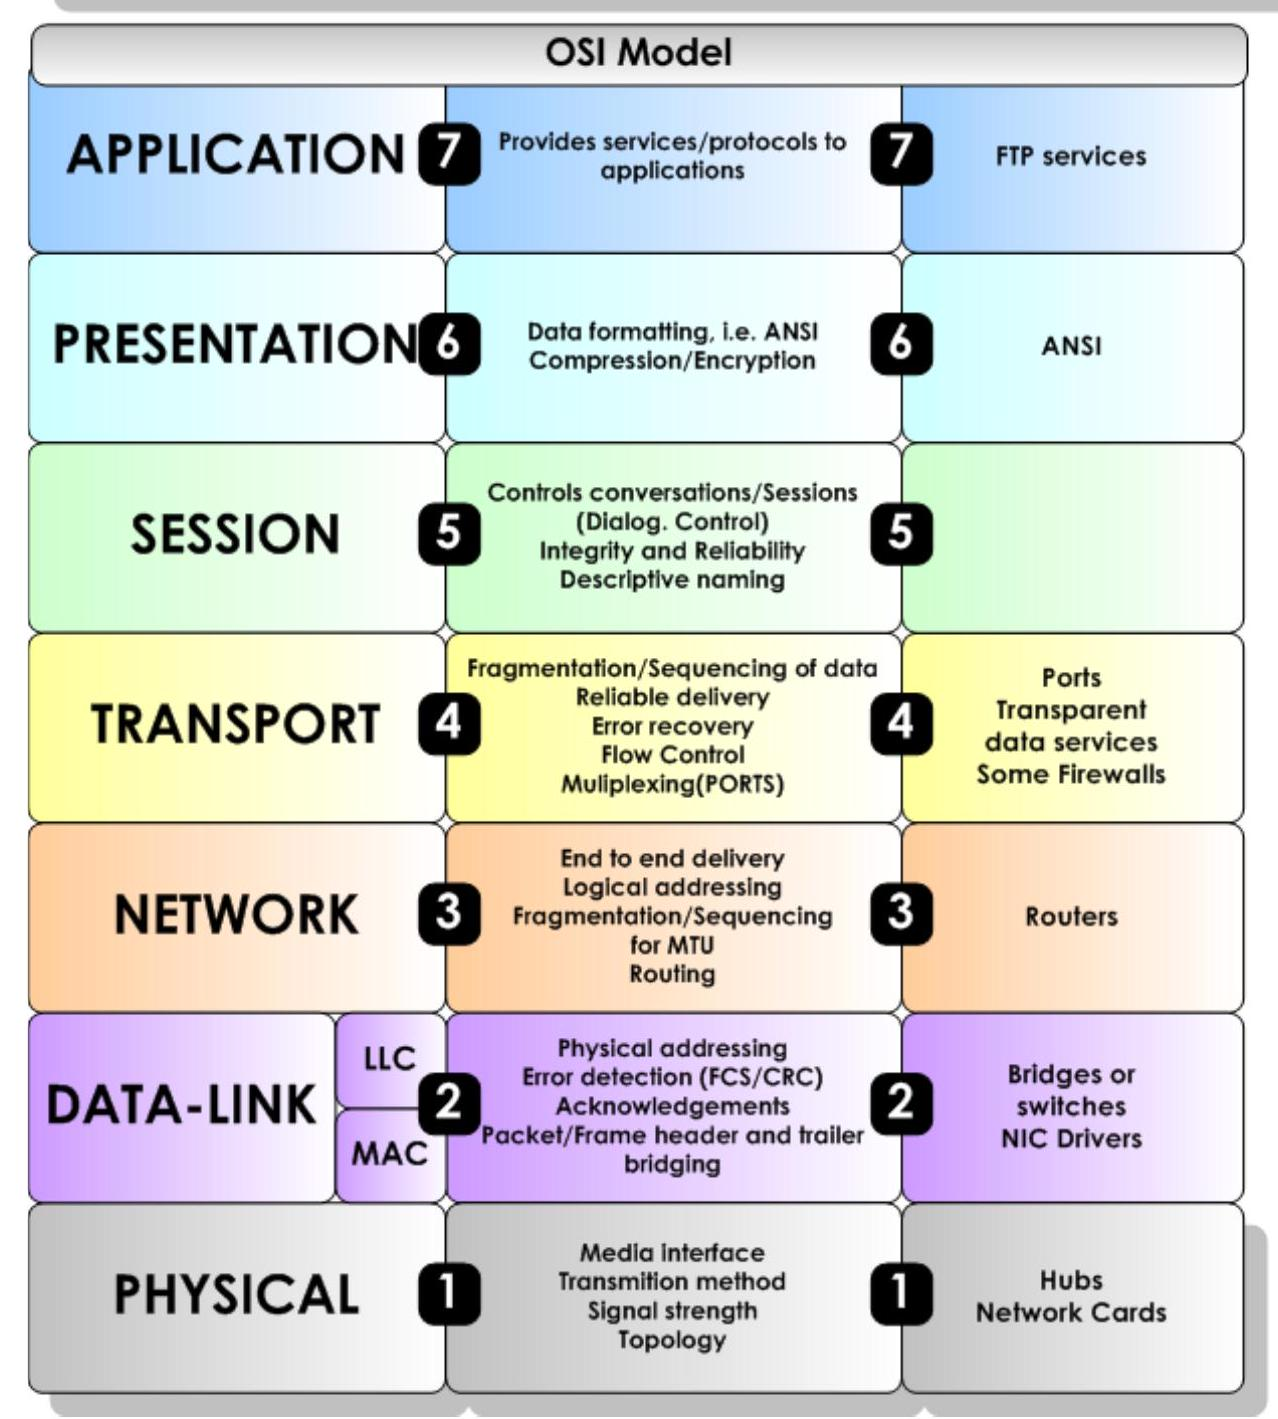
\includegraphics[max width=\textwidth]{2023_01_13_b07e3b4bcffdaab9792bg-009}
\end{center}

\begin{center}

\includegraphics[max width=\textwidth]{2023_01_13_b07e3b4bcffdaab9792bg-009(1)}
\end{center}

\begin{center}
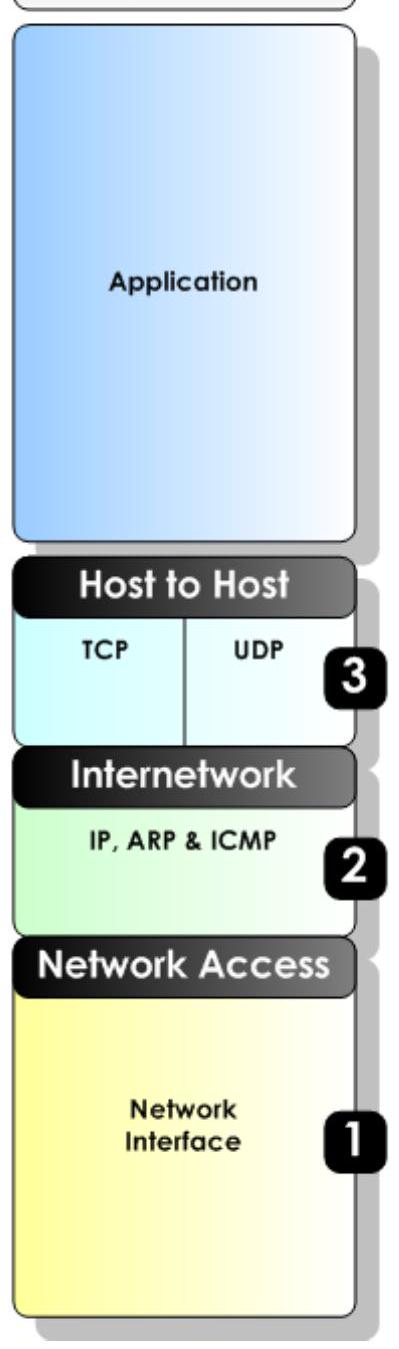
\includegraphics[max width=\textwidth]{2023_01_13_b07e3b4bcffdaab9792bg-009(2)}
\end{center}

(c) Copyright 2008 Steven Iveson WWW. \href{http://networkstuff.eu}{networkstuff.eu}

\begin{center}
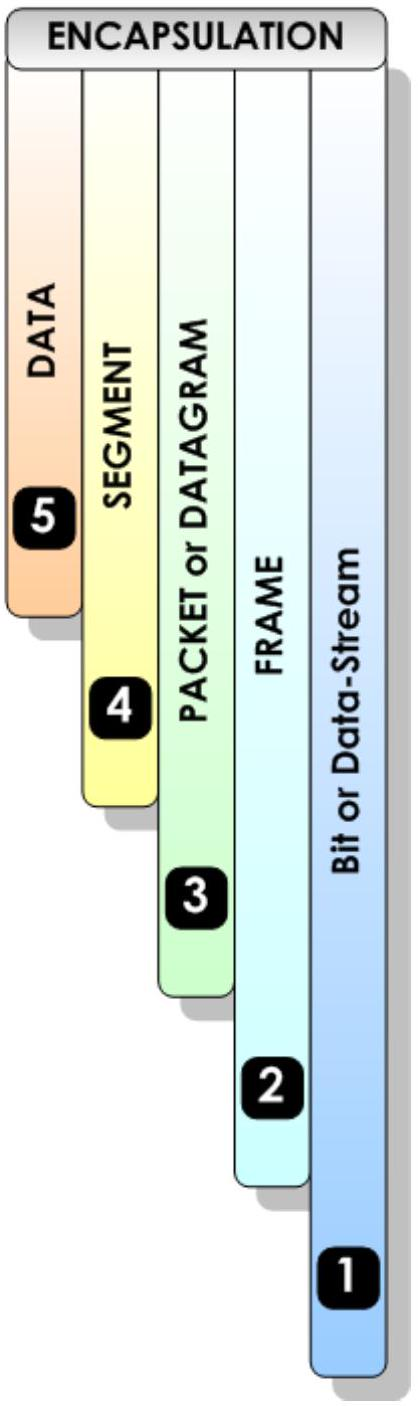
\includegraphics[max width=\textwidth]{2023_01_13_b07e3b4bcffdaab9792bg-009(3)}
\end{center}

\section{Reference Models}
Layer

Name of unit exchanged

The OSI reference model.

\begin{center}
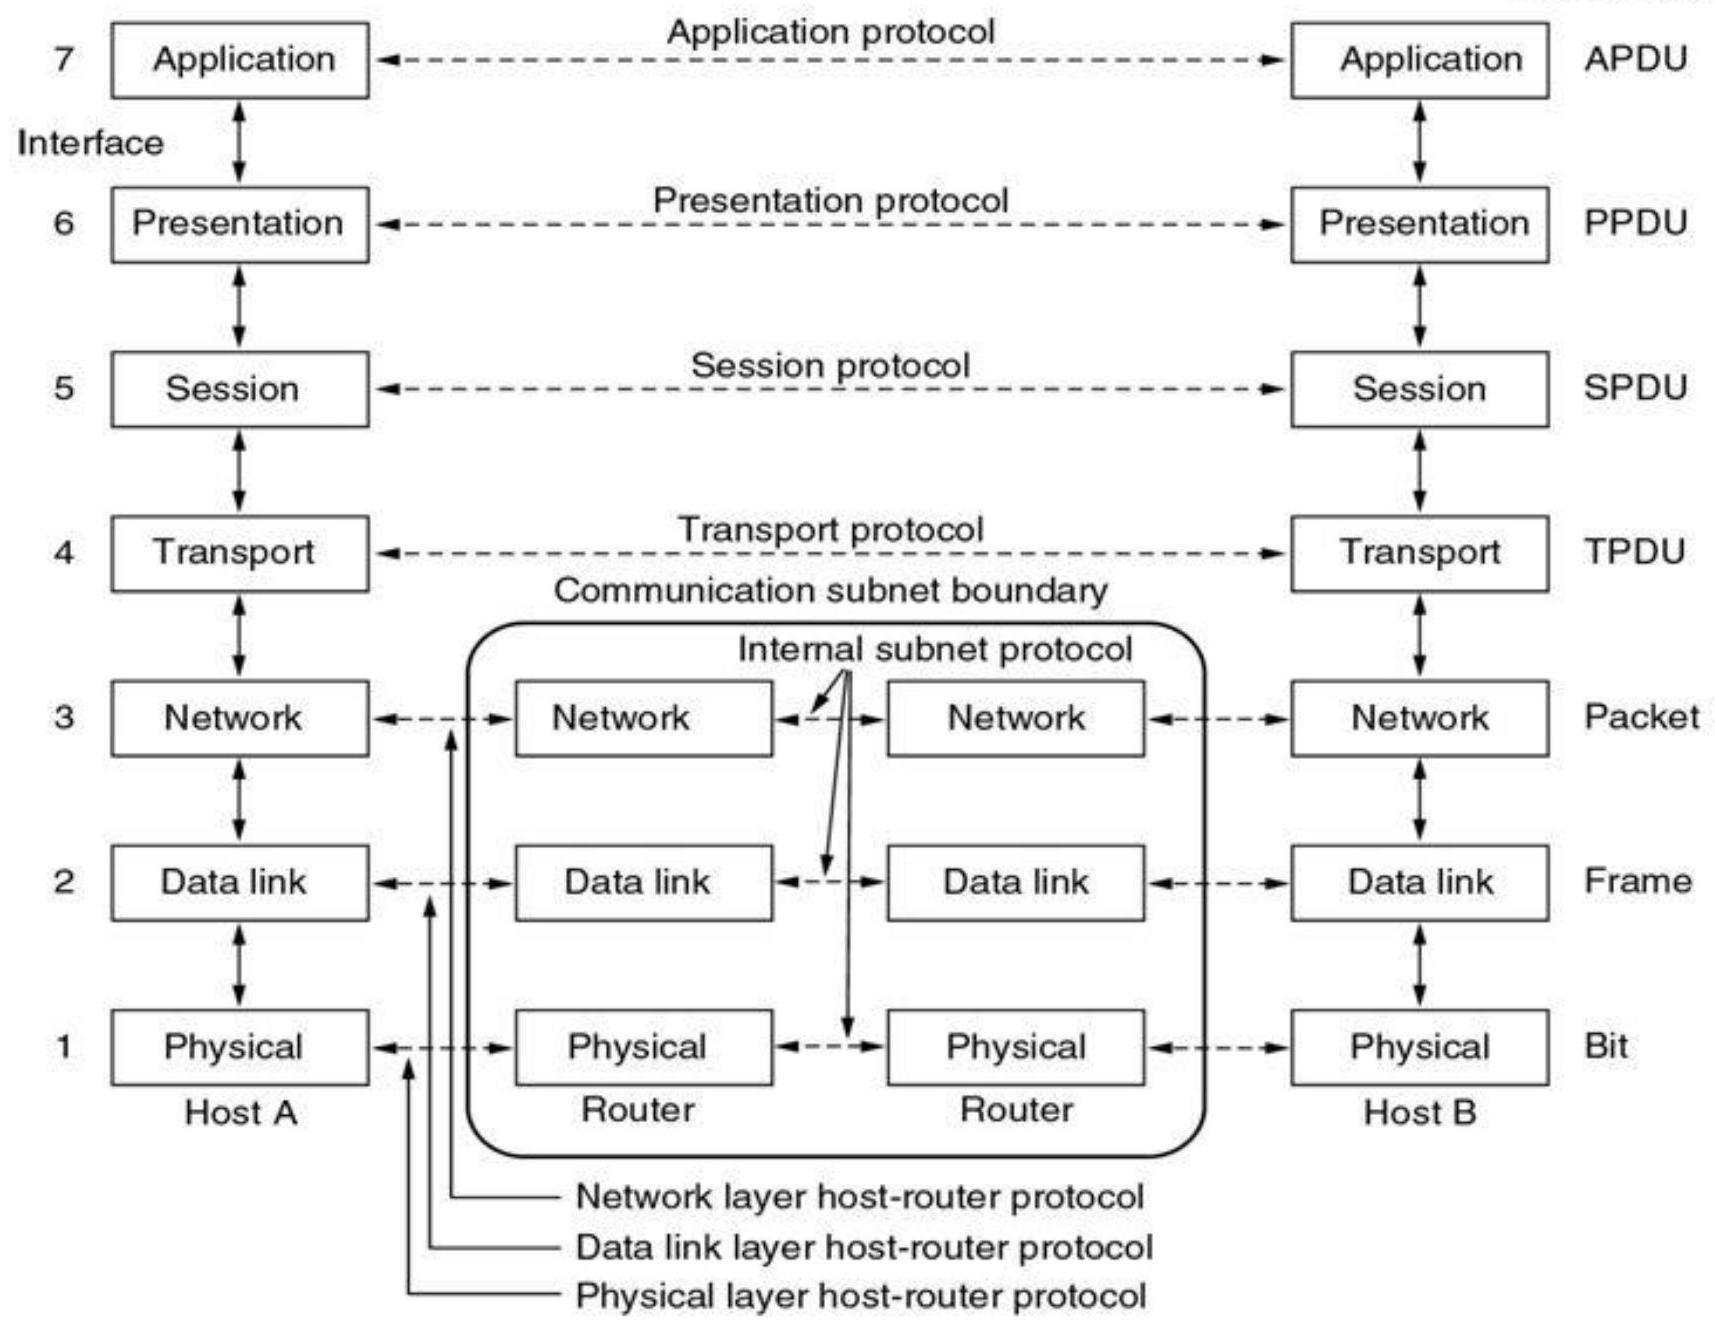
\includegraphics[max width=\textwidth]{2023_01_13_b07e3b4bcffdaab9792bg-010}
\end{center}

\section{Layer 7}
\begin{itemize}
  \item Is the top layer in the system

  \item establishes the connection between application programmes (e.g.: email, data transfer, etc.)

  \item Basic services:

\end{itemize}

o File exchange

\begin{itemize}
  \item Management protocols for user access, file access rights, electronic mail, etc.
\end{itemize}

\section{Layer 6}
\begin{itemize}
  \item It provides functions for protocol conversion, data transmission and data encryption

  \item Takes over encoding \& decoding (e.g. EBCDIC in ASCII)

  \item Takes over the definition of the formats and control characters for the exchange of the data

\end{itemize}

\section{Layer 6}
\section{- Takes care of the syntax \& correctness of the data}
\section*{Layer 5 }
\section{- Controls the establishment, execution and termination of the connection}
\textbackslash author\{

\begin{itemize}
  \item Takes over monitoring of operating parameters, data \textbackslash  flow control, reconnection in case of error and \textbackslash  synchronisation between user actions
\}
\end{itemize}

\section{$\underline{\text { Layer } 4}$}
\section{- Is the connection between application-oriented \& transport-oriented layers}
\begin{itemize}
  \item Ensures that all data packets reach the correct
recipient
\end{itemize}

\section{$\underline{\operatorname{Layer}} 4$}
\begin{itemize}
  \item Establishing the data connection between two partners, data transport, flow control, error detection and correction

  \item Ensuring completeness, uniqueness \& sequence of data blocks

  \item Their services are divided into 4 classes

\end{itemize}

\section{$\underline{\operatorname{Layer} 4}$}
\section{- Class O:}
\section{o Is the simplest}
o No error handling

o there is no error control compared to layer 3

o One transport connection corresponds to exactly one network connection

\section{Layer 4}
\section{- Class 1:}
o No error handling

o Attempts to correct errors reported by layer 3 and does not forward them to layer 5 .

o For example, if the transport connection is interrupted, an attempt can be made to rebuild it without this being noticed above layer 4 .

\section{Layer 4}
\section{- Class 2:}
\section{o can establish several transport connections (multiplex connection)}
\section{o In this case, the network connection may only be disconnected when the last transport connection has been terminated.}
\section{$\underline{\operatorname{Layer} 4}$}
\section{- Class 3 :}
\section{o Covers the services of classes 1 \& 2 (error handling \& multiplex connections)}
\section{Layer 4}
\begin{itemize}
  \item Class 4:
\end{itemize}

o Contains, in addition to the functions of class 3, additional mechanisms for error detection/handling

\begin{itemize}
  \item Especially in datagram-oriented networks (LAN), a connection-oriented service can be provided in this way (ensuring completeness, uniqueness and sequence of data blocks).
\end{itemize}

\section{Layer 4}
\begin{itemize}
  \item Devices:
\end{itemize}

o Gateway

\section{Layer 3}
\begin{itemize}
  \item is mainly used for data packet
transmission

  \item Responsible for the choice of data
paths (routing)

  \item for multiplexing several connections over individual sections

\end{itemize}

\section{Layer 3}
\begin{itemize}
  \item For error handling, flow control \& flow control between the endpoints of a connection (not between the user processes).

  \item Removal of bottlenecks (consequence of data
collisions)

\end{itemize}

\section{Layer 3}
\begin{itemize}
  \item Devices:
\end{itemize}

o Router

o Layer 3 Switch

\section{Layer 2}
\begin{itemize}
  \item Ensuring a functioning connection between two directly adjacent stations

  \item Provides a defined framework for data transport, error detection and synchronisation of data

\end{itemize}

\section{Layer 2}
\begin{itemize}
  \item Information is divided into blocks of appropriate length called frames and provided with check info for error detection/correction.

  \item Flow control for the binary data

  \item Transmitter \& receiver hardware addresses are added to the data frame

\end{itemize}

\section{Layer 2}
\begin{itemize}
  \item For local networks, this layer is subdivided again: - 2 a (Media Access Control, MAC): Controls access to the transmission medium
\end{itemize}

o 2 b (Logical Link Control, LLC): Layer 2 functions dependent on the transmission medium

\section{Layer 2}
\begin{itemize}
  \item Devices:
\end{itemize}

o Bridge

Switch

\section{Layer 1}
\begin{itemize}
  \item Is the bottom layer

  \item This is where the physical data transmission takes place

  \item It defines the electrical, mechanical \& functional parameters for the physical connection of two units (e.g. level, modulation, cable, connector, transmission rate, etc.).

\end{itemize}

\section{Layer 1}
\begin{itemize}
  \item Devices and network components:
\end{itemize}

o Antenna

o Amplifier

o Plug and socket for the mains cable

o Repeater

o $\mathrm{Hub}$

o Transceiver

o T-piece and the end resistor

\section{Communication between the layers}
Layer 7

Layer 6

\begin{center}
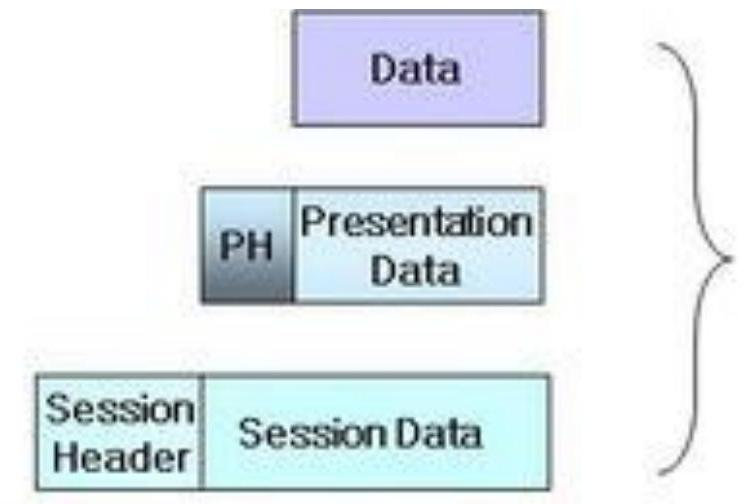
\includegraphics[max width=\textwidth]{2023_01_13_b07e3b4bcffdaab9792bg-032}
\end{center}

Layer 5

Layer 4

\begin{center}
\begin{tabular}{|c|c|}
\hline
TCP Header & TCP Data \\
\hline
MAC Header & IP Data \\
\hline
Ethernet/ Token-Ring Frame / X.25 / FR / ATM Data &  \\
\hline
\end{tabular}
\end{center}

Layer 3

Layer 1

Layer 2 TCP Frame

Application

Frame

IP Frame

MAC Frame

\section{Communication between the layers}
\begin{center}
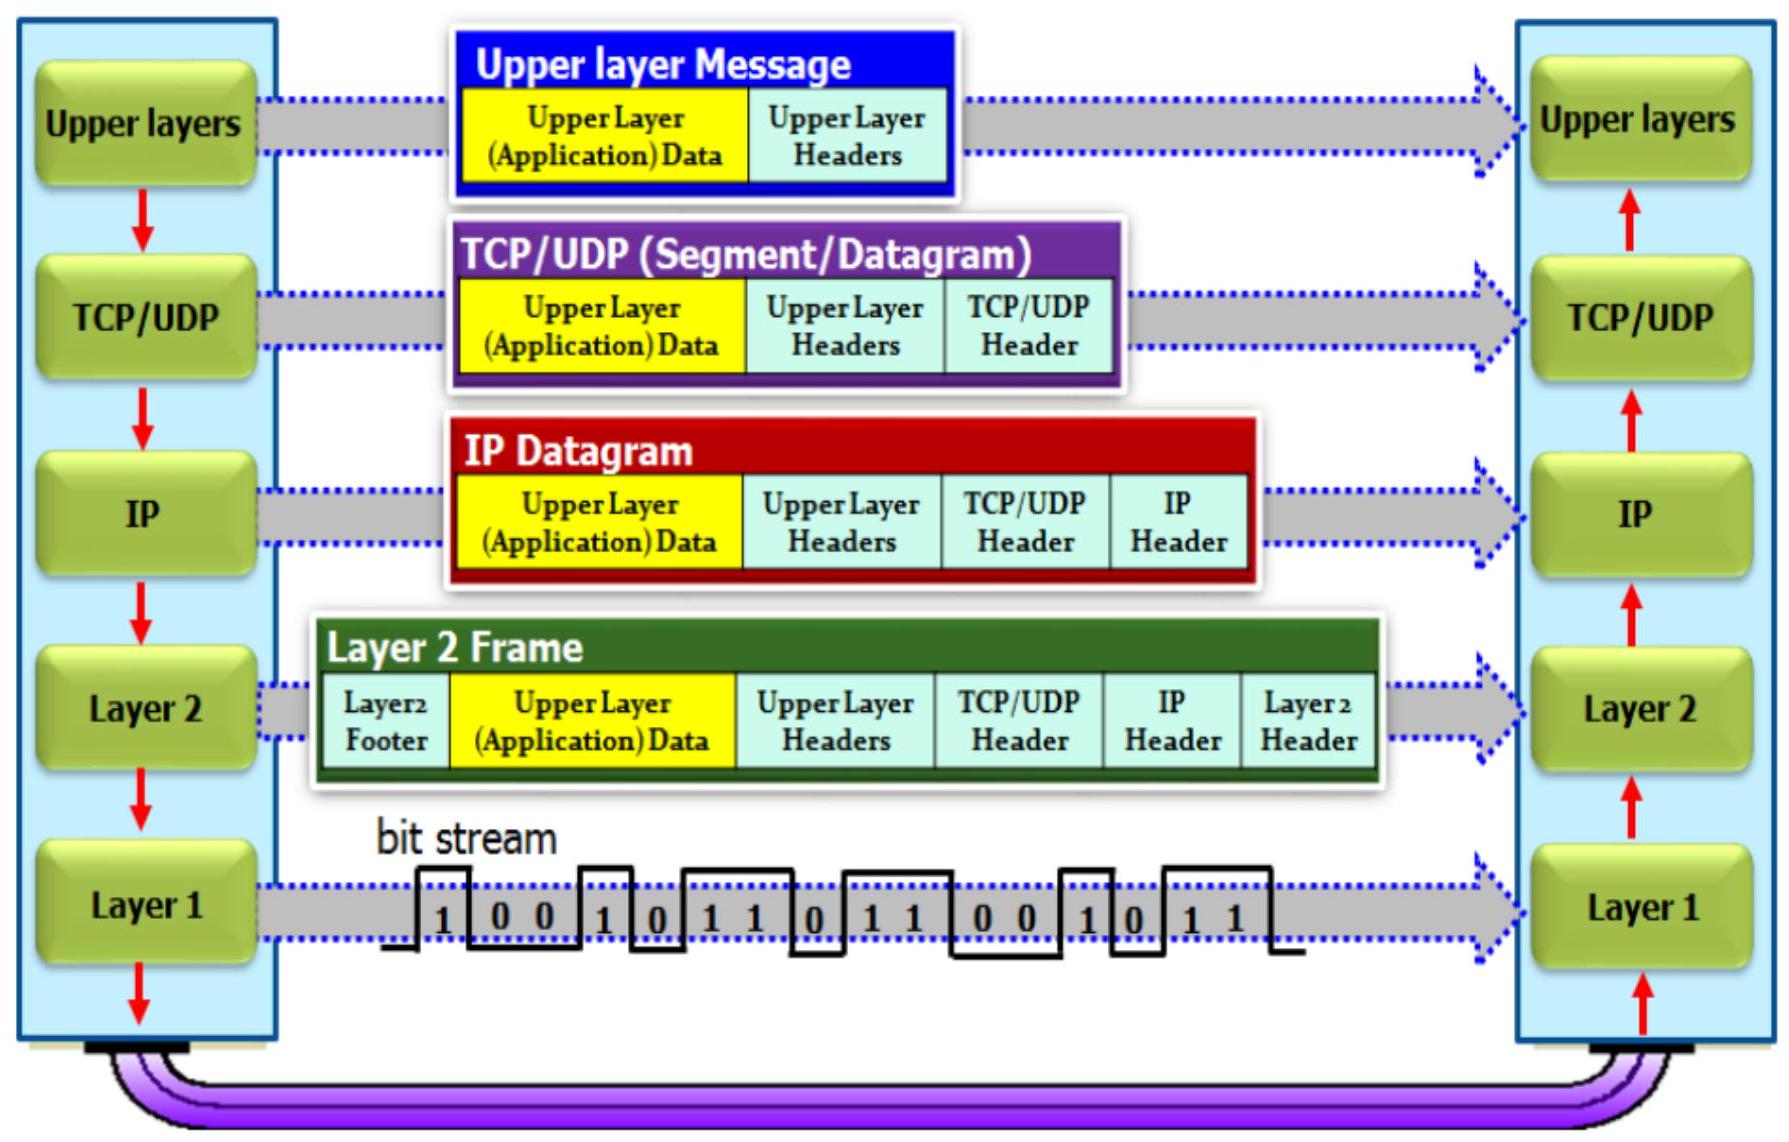
\includegraphics[max width=\textwidth]{2023_01_13_b07e3b4bcffdaab9792bg-033}
\end{center}

Figure 2. Encapsulation and Decapsulation of TCP/IP Protocol

\section{Devices}
OSI (Open Source Interconnection) 7 Layer Model

\begin{center}
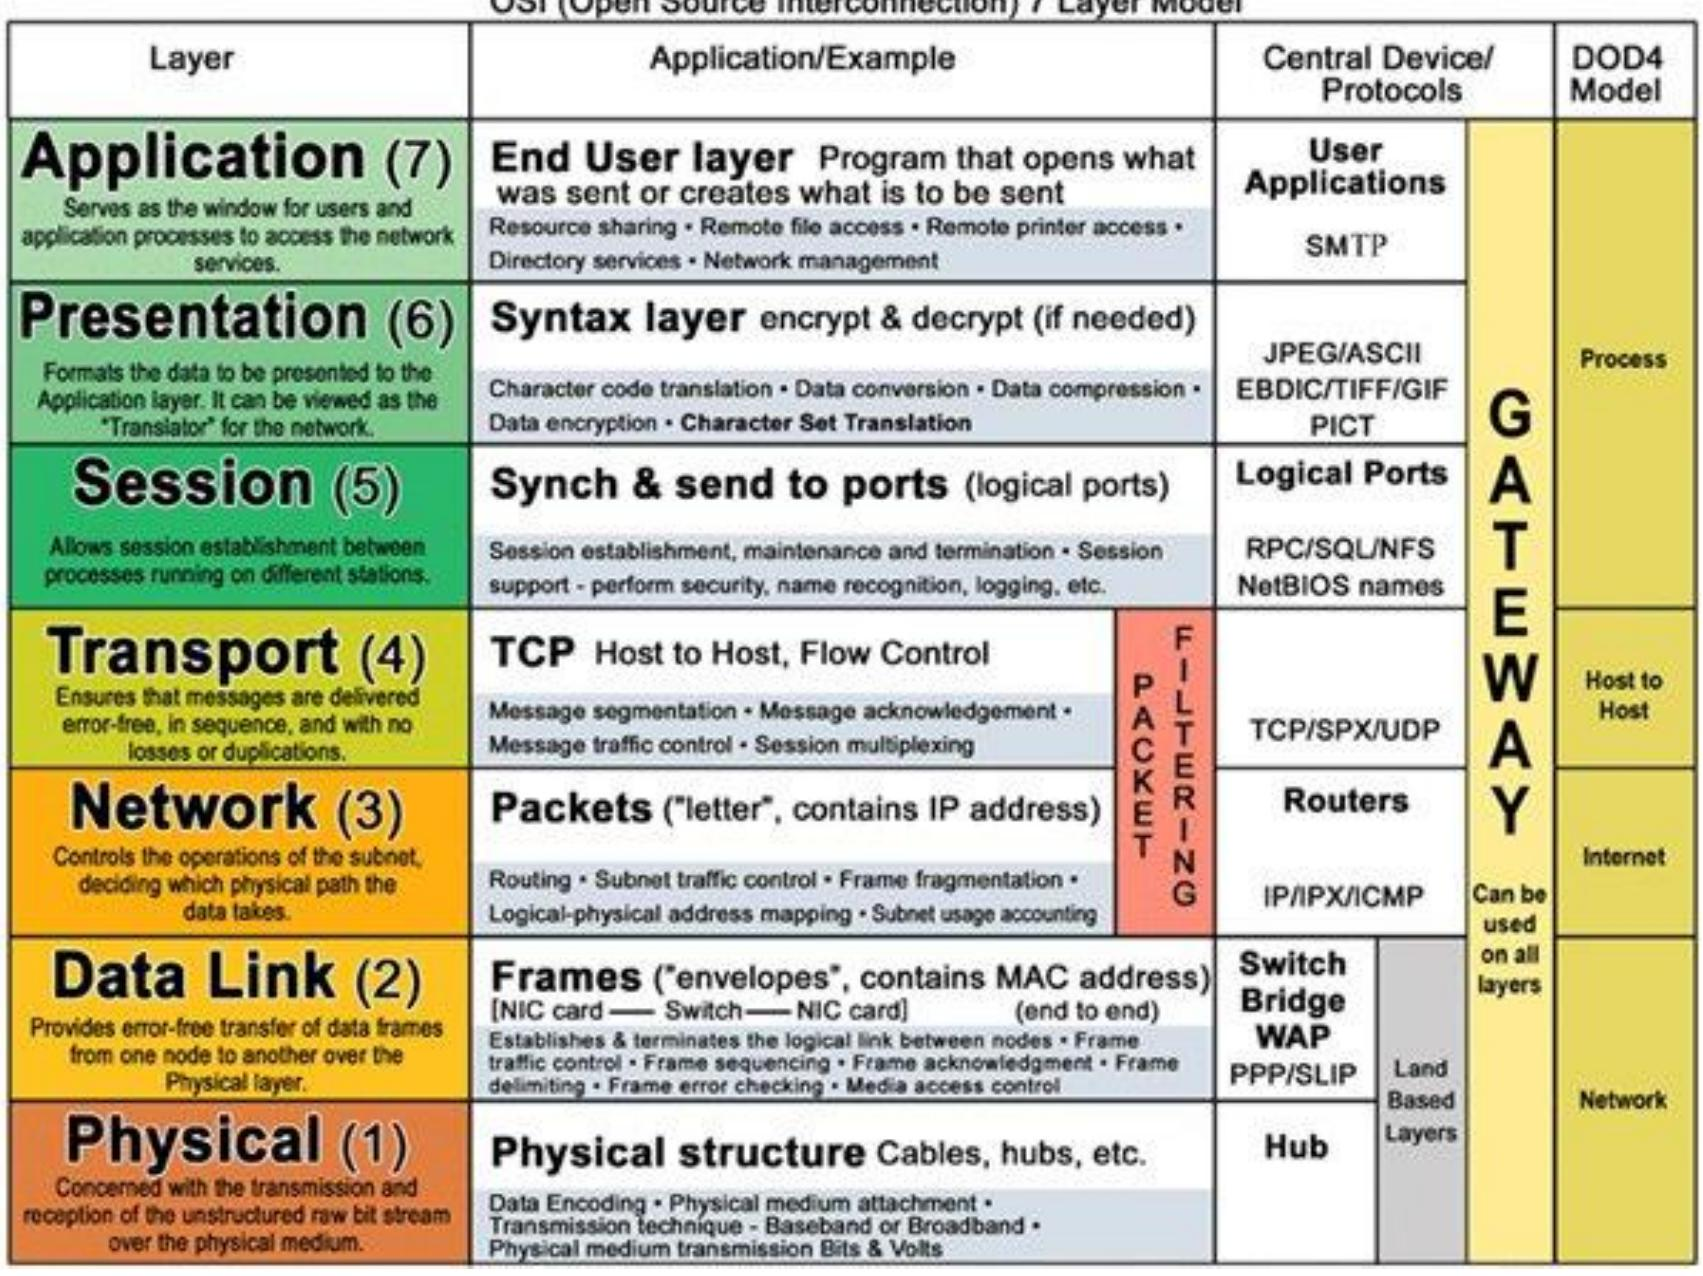
\includegraphics[max width=\textwidth]{2023_01_13_b07e3b4bcffdaab9792bg-034}
\end{center}

\section{Sources}
\begin{itemize}
  \item \href{http://www.wikipedia.de}{www.wikipedia.de} 17.12.05

  \item \href{http://homepages.luc.edu/}{http://homepages.luc.edu/} bmontes/CIEP489Images/OSI-Model.gif 17.12.05

  \item \href{http://www.netzmafia.de/skripten/netze/netzo.htm}{http://www.netzmafia.de/skripten/netze/netzo.htm} l\#0.1 17.12.05

  \item My DVT binder 2004/05

\end{itemize}

\section{Transceiver Block Diagram}
\section{Transmitter}
Signal

\begin{center}
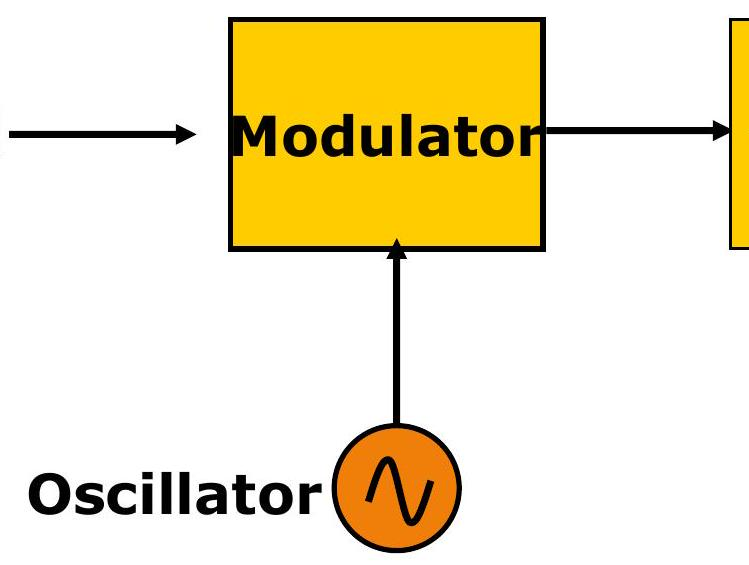
\includegraphics[max width=\textwidth]{2023_01_13_b07e3b4bcffdaab9792bg-037}
\end{center}

\begin{center}
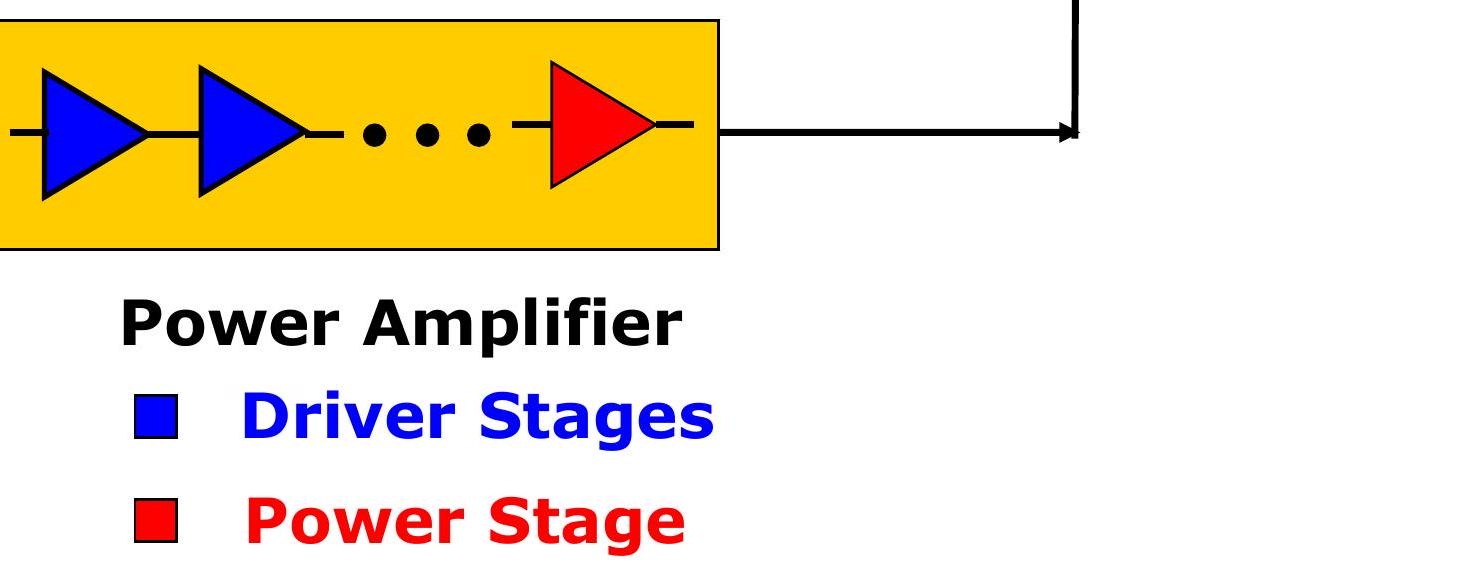
\includegraphics[max width=\textwidth]{2023_01_13_b07e3b4bcffdaab9792bg-037(1)}
\end{center}

\section{Receiver}
Antenna

\section{Low Noise Amplifier}
\begin{center}
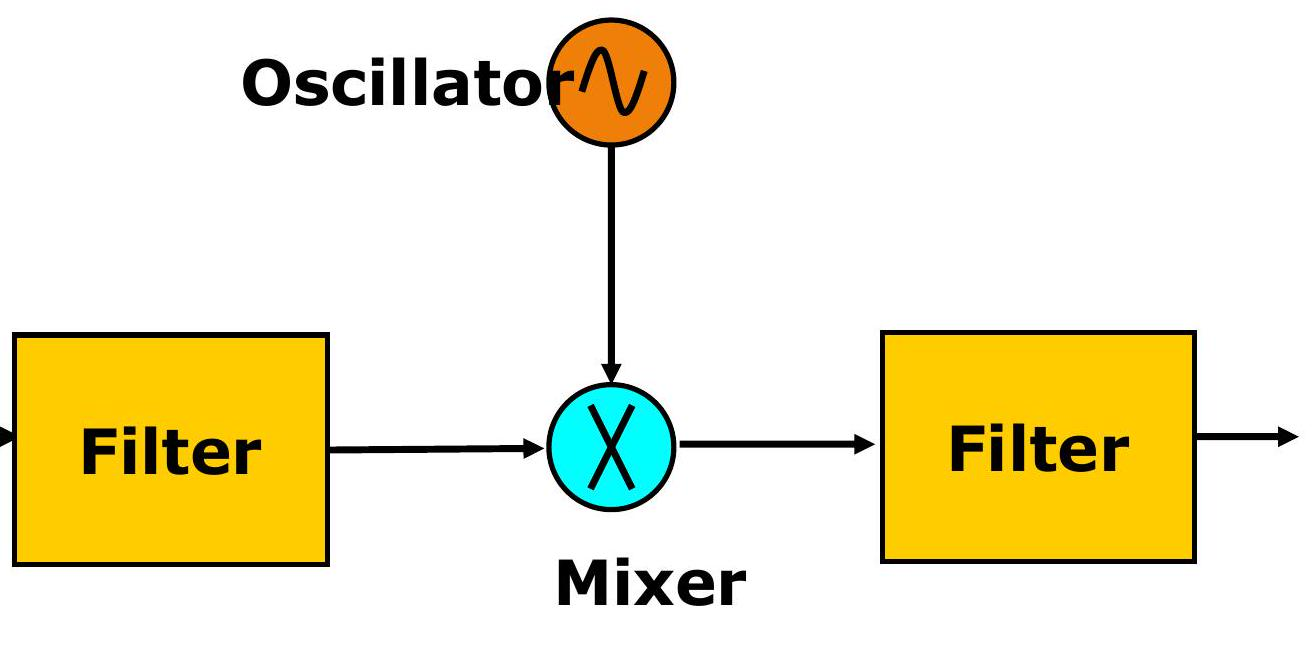
\includegraphics[max width=\textwidth]{2023_01_13_b07e3b4bcffdaab9792bg-038}
\end{center}

$\square$ Low Noise Amplifier

Gain-Stage Amplifier

\section{Transceiver $=$ Transmitter $+$ Receiver}
\begin{center}
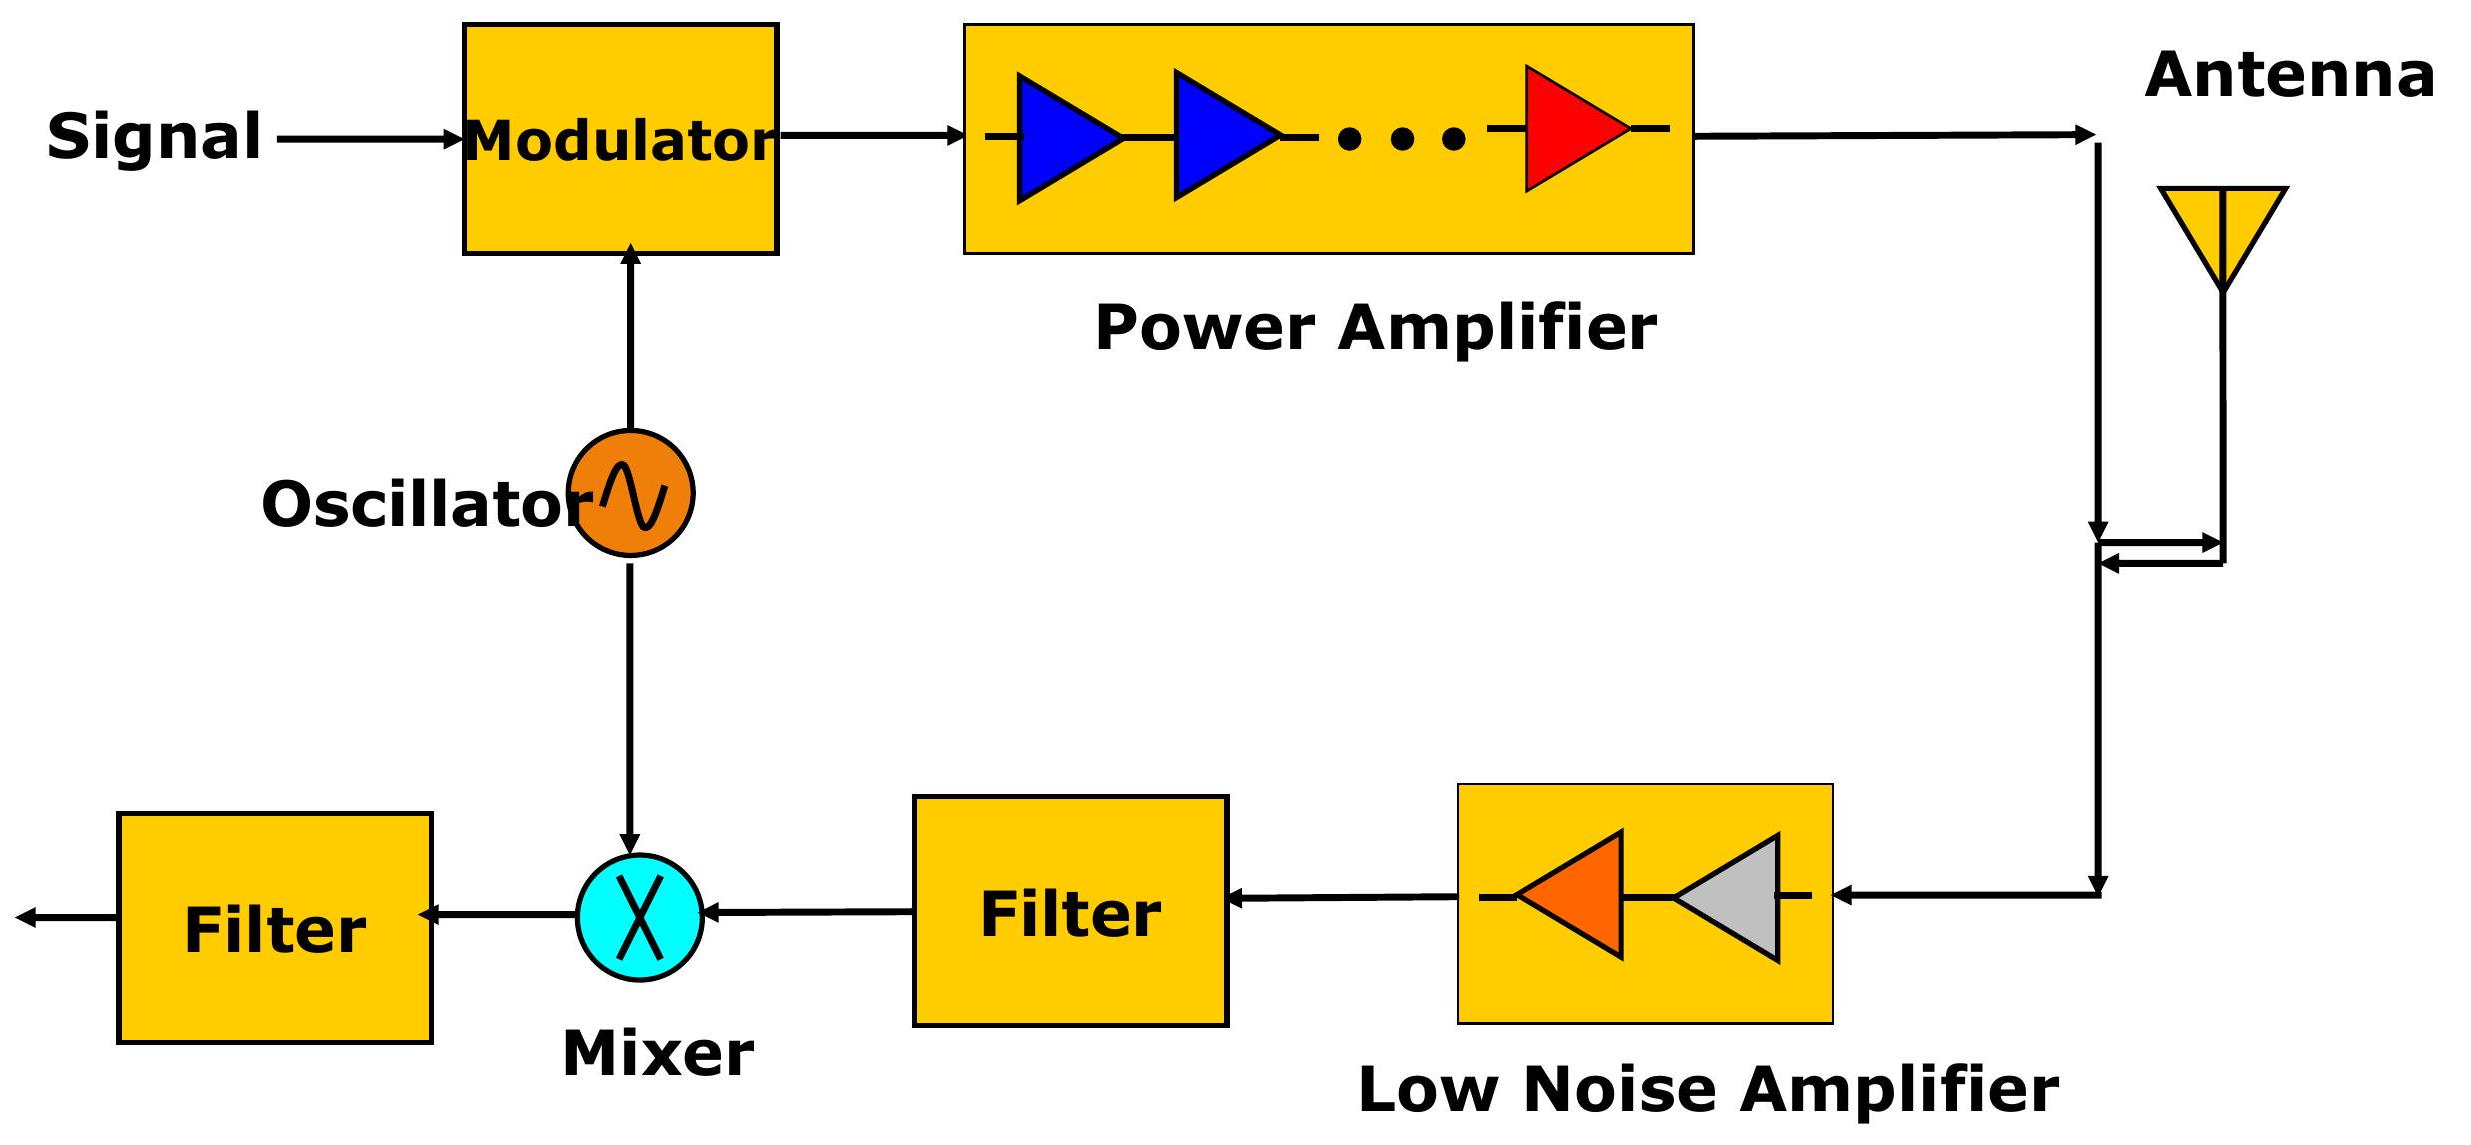
\includegraphics[max width=\textwidth]{2023_01_13_b07e3b4bcffdaab9792bg-039}
\end{center}

\section{Signal Encoding Techniques}
\section{Encoding Techniques}
\begin{itemize}
  \item Digital data, digital signal

  \item Analog data, digital signal

  \item Digital data, analog signal

  \item Analog data, analog signal

\end{itemize}

\section{Digital Data, Digital Signal}
\begin{itemize}
  \item Digital signal

  \item Discrete, discontinuous voltage pulses

\end{itemize}

o Each pulse is a signal element

\begin{itemize}
  \item Binary data encoded into signal elements
\end{itemize}

\section{Terms (1)}
\begin{itemize}
  \item Unipolar
\end{itemize}

All signal elements have same sign

\begin{itemize}
  \item Polar

  \item One logic state represented by positive voltage the other by negative voltage

  \item Data rate

\end{itemize}

o Rate of data transmission in bits per second

\begin{itemize}
  \item Duration or length of a bit
\end{itemize}

o Time taken for transmitter to emit the bit

\section{Terms (2)}
\begin{itemize}
  \item Modulation rate

  \item Rate at which the signal level changes

  \item Measured in baud = signal elements per second

  \item Mark and Space

\end{itemize}

o Binary 1 and Binary o respectively

\section{Interpreting Signals}
\begin{itemize}
  \item Need to know
\end{itemize}

o Timing of bits - when they start and end o Signal levels

\begin{itemize}
  \item Factors affecting successful interpreting of signals o Signal to noise ratio
\end{itemize}

o Data rate

o Bandwidth

\section{Comparison of Encoding Schemes (1)}
\begin{itemize}
  \item Signal Spectrum

  \item Lack of high frequencies reduces required bandwidth

  \item Lack of dc component allows ac coupling via transformer, providing isolation

\end{itemize}

o Concentrate power in the middle of the bandwidth

\section{- Clocking}
o Synchronizing transmitter and receiver

o External clock

o Sync mechanism based on signal

\section{Comparison of Encoding Schemes (2)}
\begin{itemize}
  \item Error detection

  \item Can be built in to signal encoding

  \item Signal interference and noise immunity

\end{itemize}

o Some codes are better than others

\begin{itemize}
  \item Cost and complexity

  \item Higher signal rate (\& thus data rate) lead to higher costs

\end{itemize}

o Some codes require signal rate greater than data rate

\section{Encoding Schemes}
\begin{itemize}
  \item Nonreturn to Zero-Level (NRZ-L)

  \item Nonreturn to Zero Inverted (NRZI)

  \item Bipolar -AMI

  \item Pseudoternary

  \item Manchester

  \item Differential Manchester

  \item B8ZS

  \item $\mathrm{HDB}_{3}$

\end{itemize}

\section{Nonreturn to Zero-Level (NRZ-L)}
\begin{itemize}
  \item Two different voltages for 0 and 1 bits

  \item Voltage constant during bit interval o no transition I.e. no return to zero voltage

  \item e.g. Absence of voltage for zero, constant positive voltage for one

  \item More often, negative voltage for one value and positive for the other

  \item This is NRZ-L

\end{itemize}

\section{Nonreturn to Zero Inverted}
\begin{itemize}
  \item Nonreturn to zero inverted on ones

  \item Constant voltage pulse for duration of bit

  \item Data encoded as presence or absence of signal transition at beginning of bit time

  \item Transition (low to high or high to low) denotes a binary 1

  \item No transition denotes binary o

  \item An example of differential encoding

\end{itemize}

\begin{center}
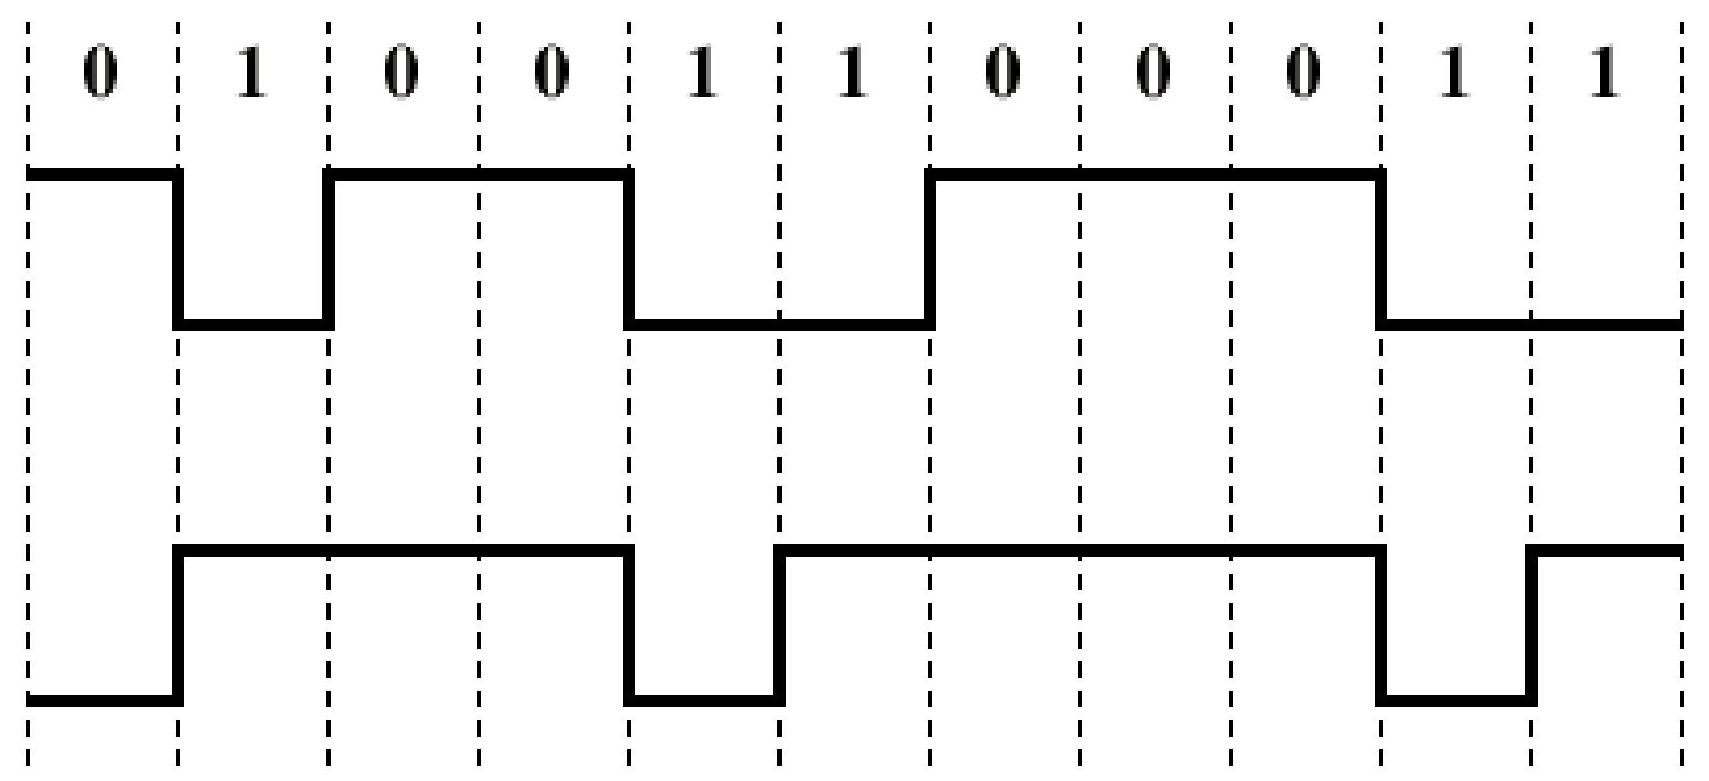
\includegraphics[max width=\textwidth]{2023_01_13_b07e3b4bcffdaab9792bg-051}
\end{center}

\section{Differential Encoding}
\begin{itemize}
  \item Data represented by changes rather than levels

  \item More reliable detection of transition rather than level

  \item In complex transmission layouts it is easy to lose sense of polarity

\end{itemize}

\section{NRZ pros and cons}
\begin{itemize}
  \item Pros
\end{itemize}

o Easy to engineer

\begin{itemize}
  \item Make good use of bandwidth

  \item Cons

\end{itemize}

o dc component

o Lack of synchronization capability

\begin{itemize}
  \item Used for magnetic recording

  \item Not often used for signal transmission

\end{itemize}

\section{Multilevel Binary}
\begin{itemize}
  \item Use more than two levels

  \item Bipolar-AMI

\end{itemize}

o zero represented by no line signal

o one represented by positive or negative pulse

o one pulses alternate in polarity

\begin{itemize}
  \item No loss of sync if a long string of ones (zeros still a problem)
\end{itemize}

o No net dc component

o Lower bandwidth

o Easy error detection

\section{Pseudoternary}
\begin{itemize}
  \item One represented by absence of line signal

  \item Zero represented by alternating positive and negative

  \item No advantage or disadvantage over bipolar-AMI

\end{itemize}

\section{Bipolar-AMI and Pseudoternary}
\section{Bipolar-AMI}
(most recent preceding 1 bit has negative voltage)

\section{Pseudoternary}
(most recent preceding 0 bit has negative voltage)

\begin{center}
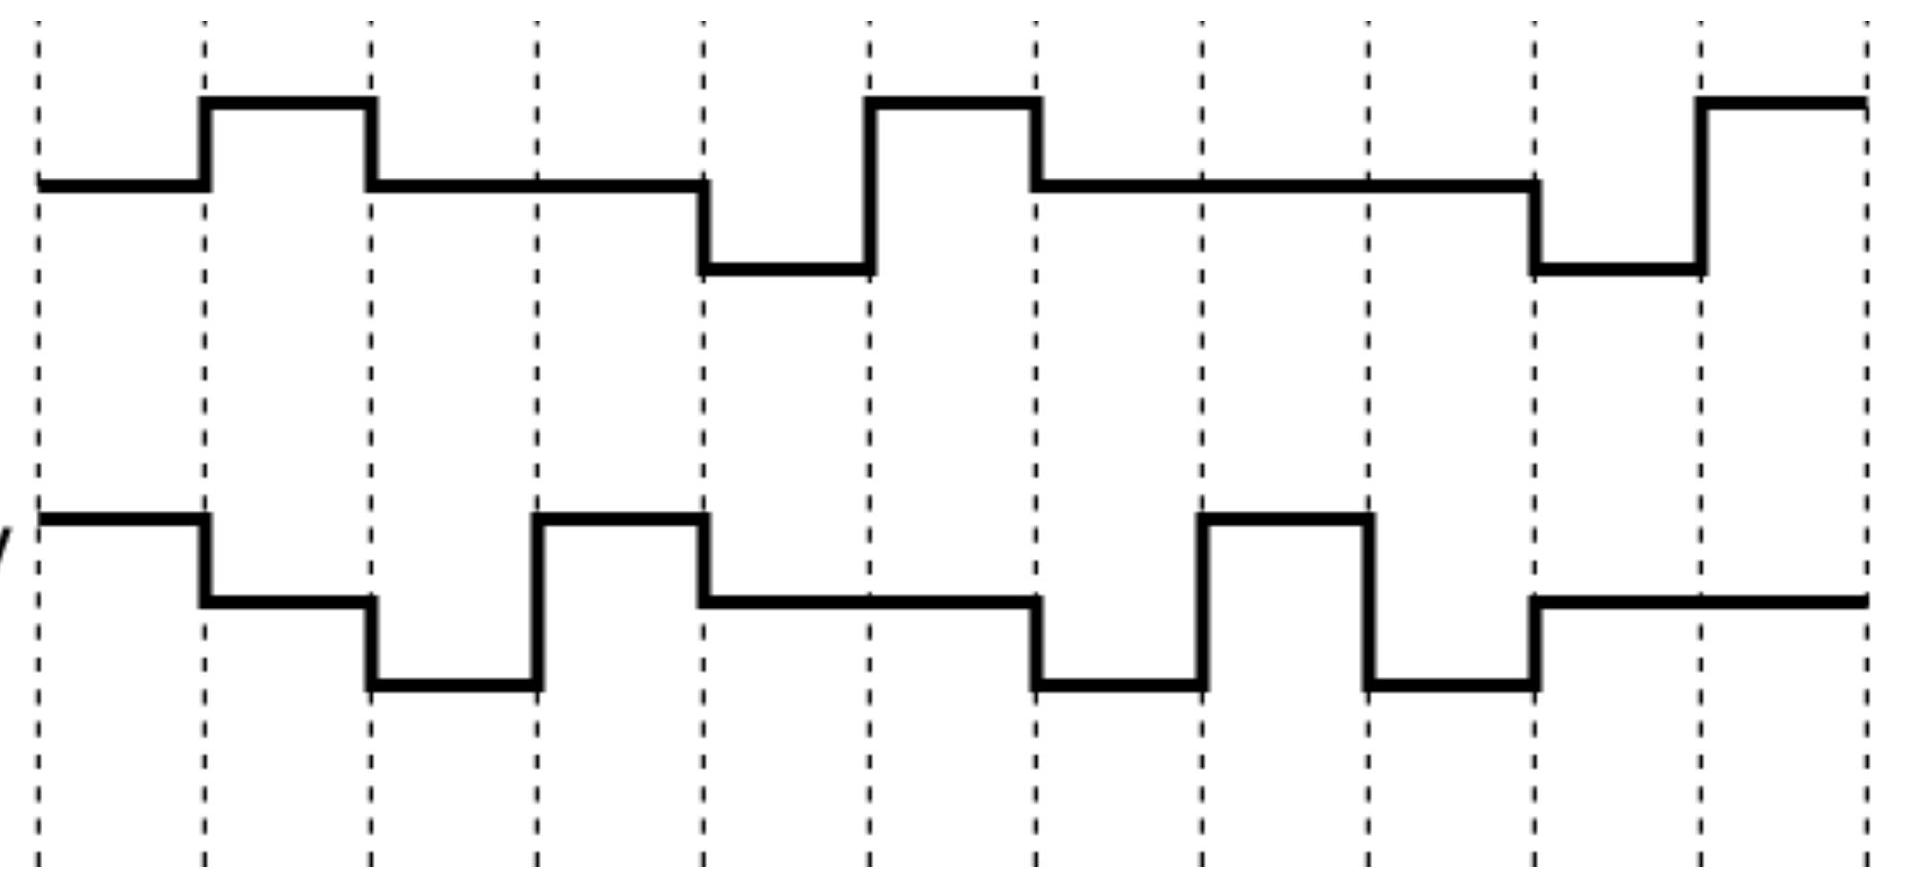
\includegraphics[max width=\textwidth]{2023_01_13_b07e3b4bcffdaab9792bg-056}
\end{center}

\section{Trade Off for Multilevel Binary}
\begin{itemize}
  \item Not as efficient as NRZ
\end{itemize}

o Each signal element only represents one bit

o In a 3 level system could represent $\log _{2} 3=1.58$ bits

\begin{itemize}
  \item Receiver must distinguish between three levels $(+\mathrm{A},-\mathrm{A}, \mathrm{o})$

  \item Requires approx. $3 \mathrm{~dB}$ more signal power for same probability of bit error

\end{itemize}

\section{Biphase}
\begin{itemize}
  \item Manchester
\end{itemize}

o Transition in middle of each bit period

o Transition serves as clock and data

o Low to high represents one

o High to low represents zero

o Used by IEEE 802.3

\begin{itemize}
  \item Differential Manchester
\end{itemize}

o Midbit transition is clocking only

o Transition at start of a bit period represents zero

o No transition at start of a bit period represents one

o Note: this is a differential encoding scheme

o Used by IEEE 802.5

\section{Manchester Encoding}
\section{Manchester Encoding}
\begin{center}
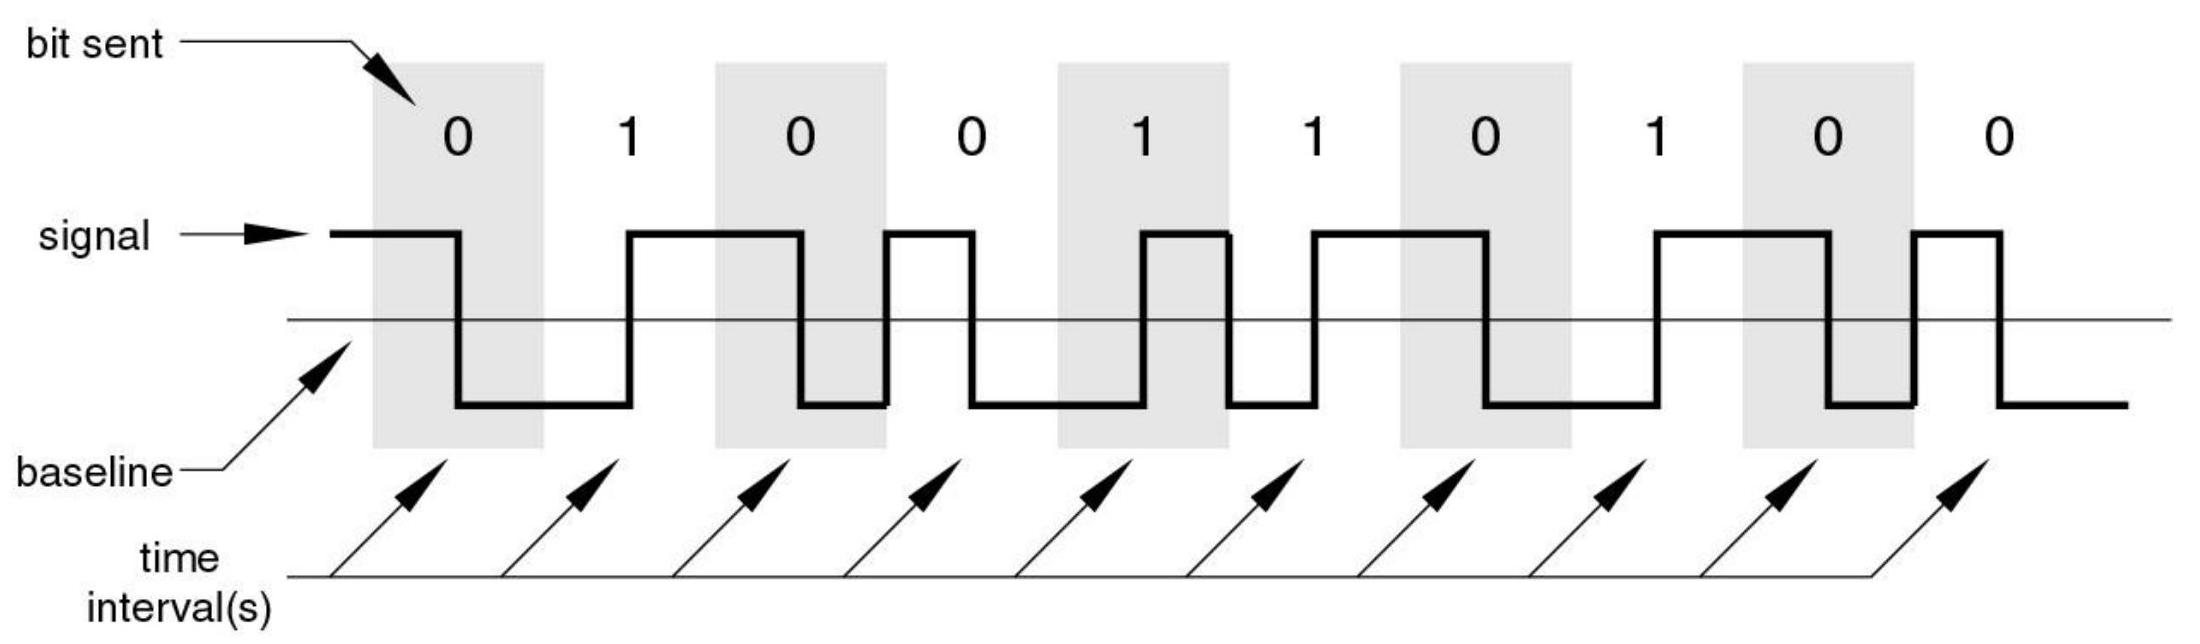
\includegraphics[max width=\textwidth]{2023_01_13_b07e3b4bcffdaab9792bg-059}
\end{center}

\section{Differential Manchester Encoding}
\section{Differential Manchester Encoding}
\begin{center}
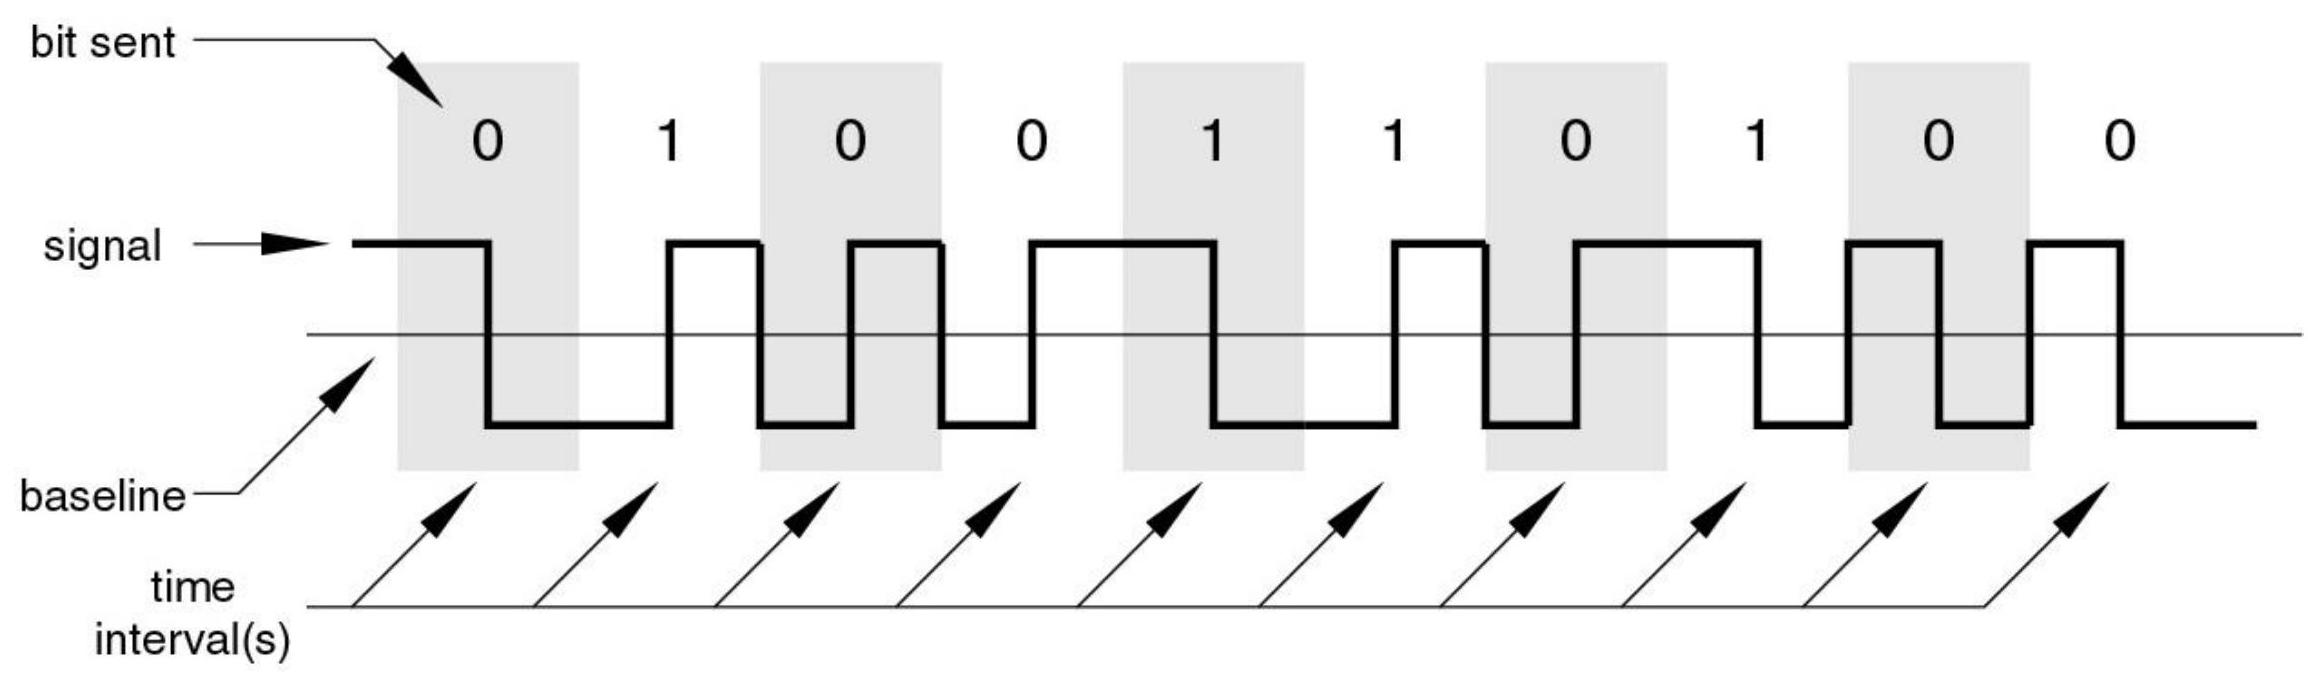
\includegraphics[max width=\textwidth]{2023_01_13_b07e3b4bcffdaab9792bg-060}
\end{center}

\section*{Biphase Pros and Cons }
\section{- Con}
\section{At least one transition per bit time and possibly two 
 - Maximum modulation rate is twice NRZ 
 o Requires more bandwidth}
\section{- Pros}


\section{Modulation Rate}
5 bits $=5 \mu \mathrm{sec}$

\begin{center}
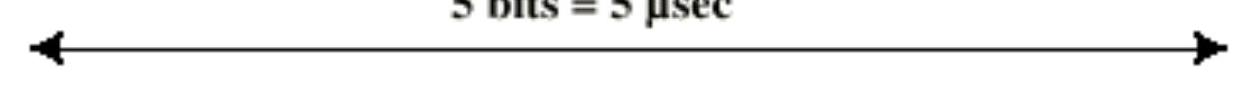
\includegraphics[max width=\textwidth]{2023_01_13_b07e3b4bcffdaab9792bg-062}
\end{center}

1

1

1

1

1

NRZI
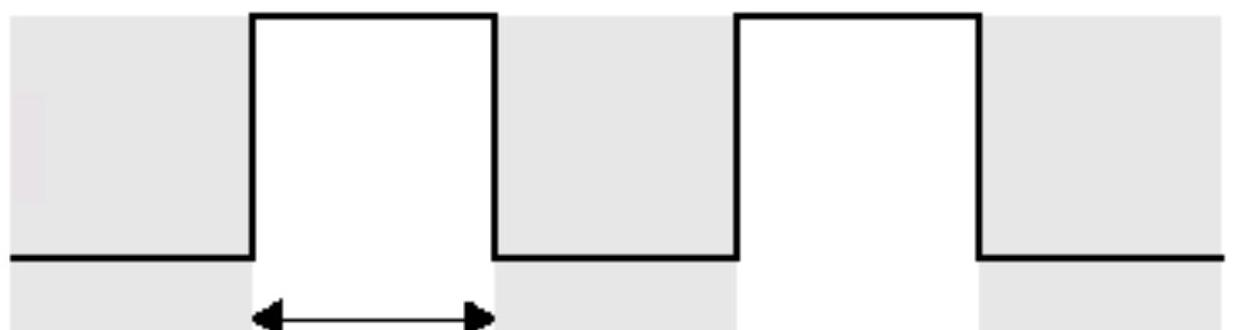
\includegraphics[max width=\textwidth, center]{2023_01_13_b07e3b4bcffdaab9792bg-062(1)}

Manchester

1 bit $=$

1 signal element $=$

1 μ $\mathrm{sec}$

\begin{center}
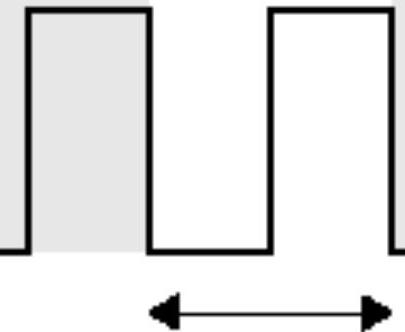
\includegraphics[max width=\textwidth]{2023_01_13_b07e3b4bcffdaab9792bg-062(2)}
\end{center}

$1 \mathrm{bit}=$

l $\mu$ sec

\begin{center}
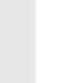
\includegraphics[max width=\textwidth]{2023_01_13_b07e3b4bcffdaab9792bg-062(3)}
\end{center}

\begin{center}
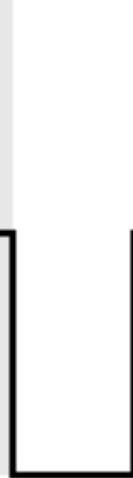
\includegraphics[max width=\textwidth]{2023_01_13_b07e3b4bcffdaab9792bg-062(4)}
\end{center}

1

1 signal element $=$

$0.5 \mu \mathrm{sec}$

\section{Scrambling}
\begin{itemize}
  \item Use scrambling to replace sequences that would produce constant voltage

  \item Filling sequence

  \item Must produce enough transitions to sync

  \item Must be recognized by receiver and replace with original

  \item Same length as original

  \item No dc component

  \item No long sequences of zero level line signal

  \item No reduction in data rate

  \item Error detection capability

\end{itemize}

\section{B8ZS}
\begin{itemize}
  \item Bipolar With 8 Zeros Substitution

  \item Based on bipolar-AMI

  \item If octet of all zeros and last voltage pulse preceding was positive encode as $000+-0-+$

  \item If octet of all zeros and last voltage pulse preceding was negative encode as 000-+0+-

  \item Causes two violations of AMI code

  \item Unlikely to occur as a result of noise

  \item Receiver detects and interprets as octet of all zeros

\end{itemize}

\section{$\mathrm{HDB}_{3}$}
\begin{itemize}
  \item High Density Bipolar 3 Zeros

  \item Based on bipolar-AMI

  \item String of four zeros replaced with one or two pulses

\end{itemize}

\section{B8ZS and $\mathrm{HDB}_{3}$}
\begin{center}
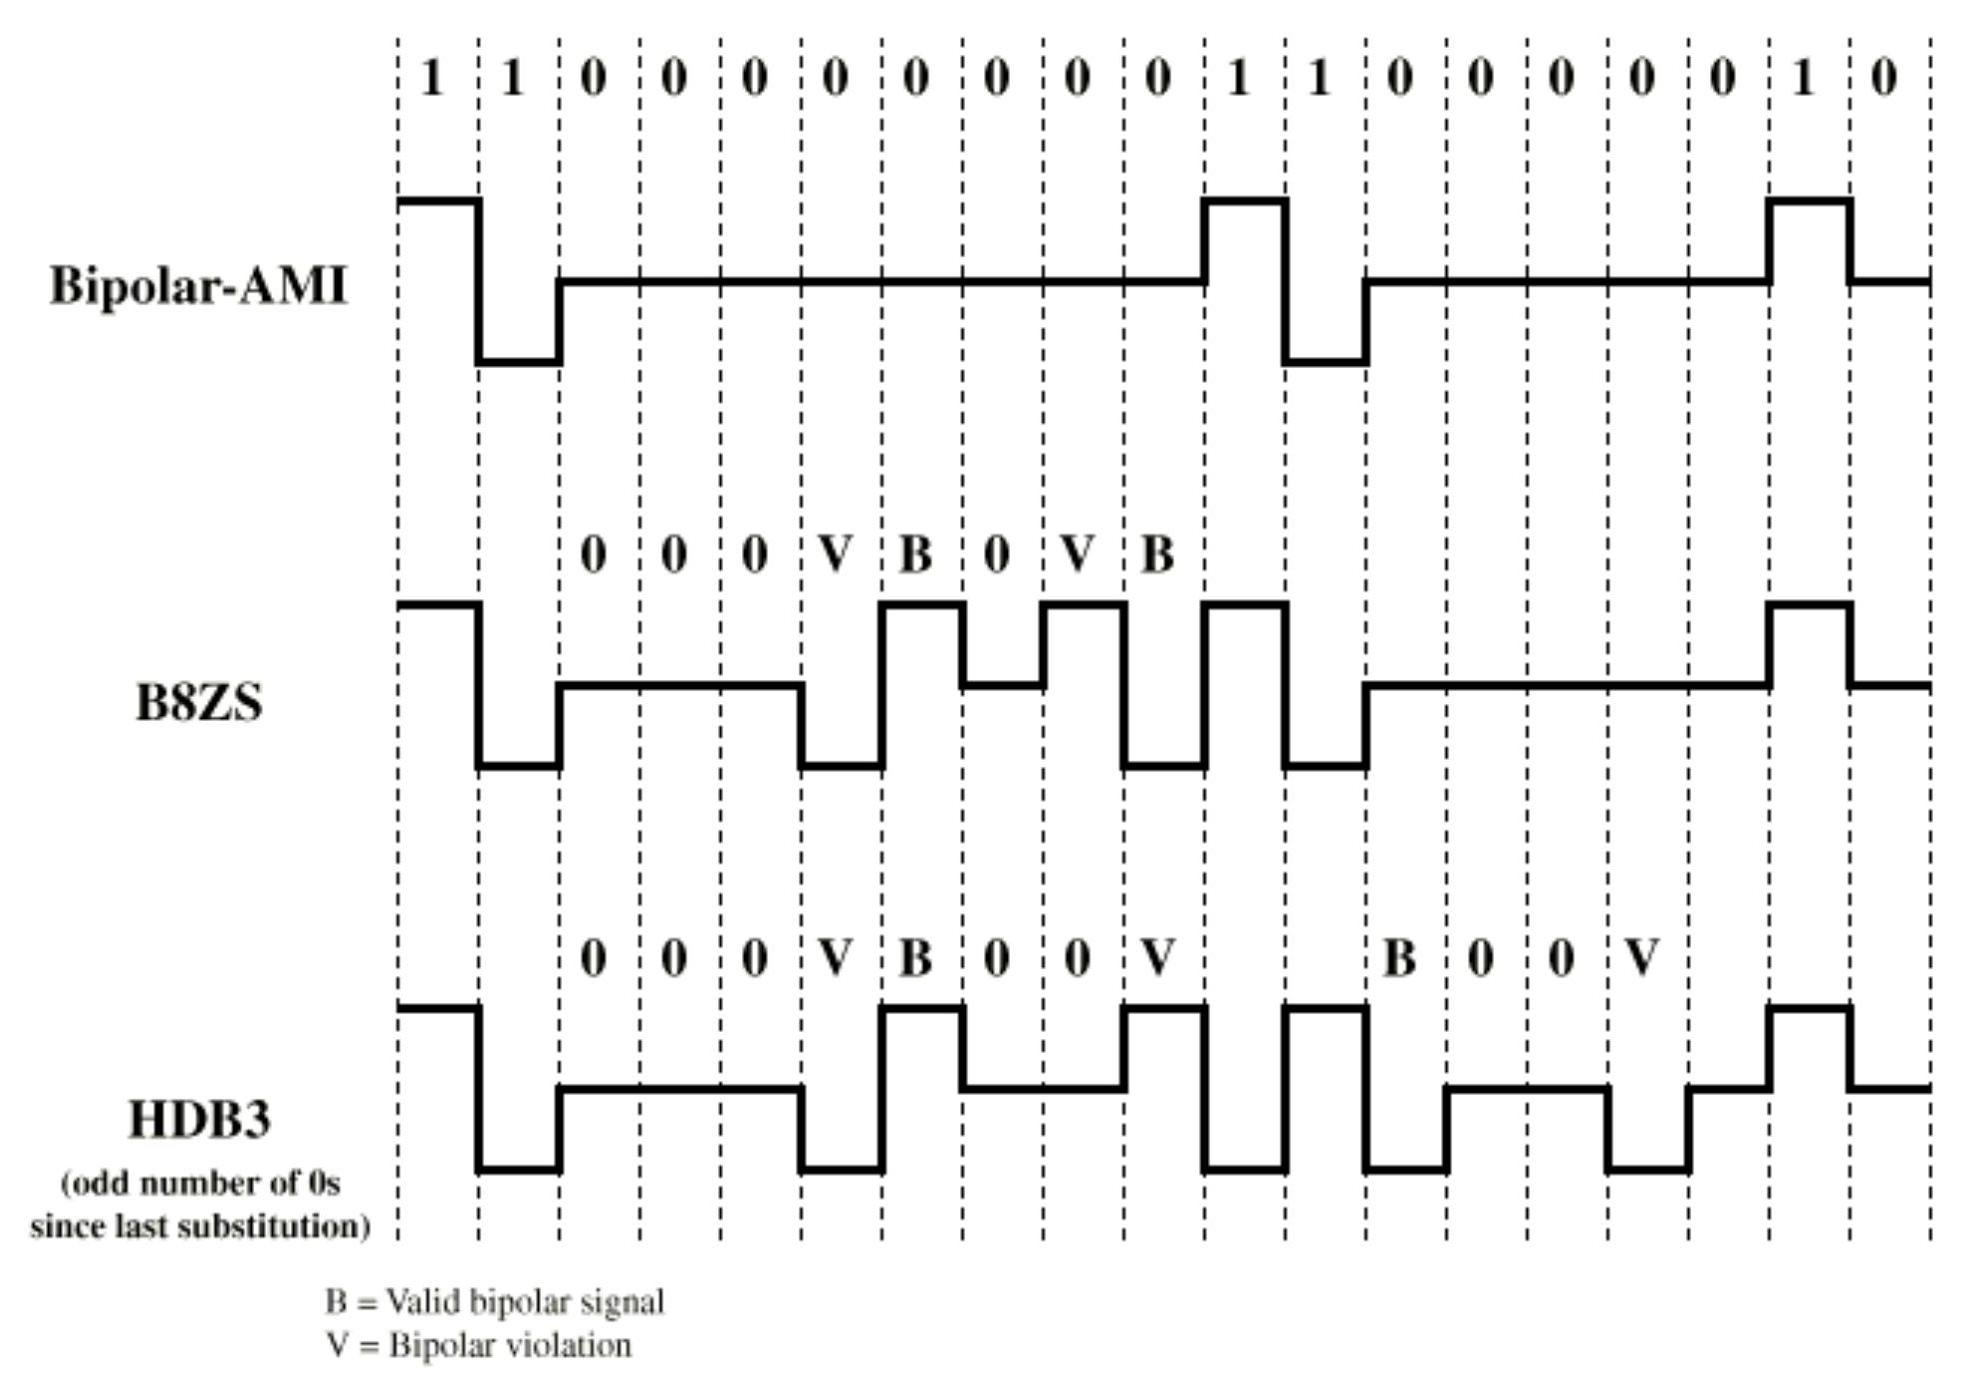
\includegraphics[max width=\textwidth]{2023_01_13_b07e3b4bcffdaab9792bg-066}
\end{center}

\section{Digital Data, Analog Signal}
\begin{itemize}
  \item Public telephone system o $300 \mathrm{~Hz}$ to $3400 \mathrm{~Hz}$
\end{itemize}

o Use modem (modulator-demodulator)

\begin{itemize}
  \item Amplitude shift keying (ASK)

  \item Frequency shift keying (FSK)

  \item Phase shift keying (PK)

\end{itemize}

\section{Modulation Techniques}
(a) ASK

\begin{center}
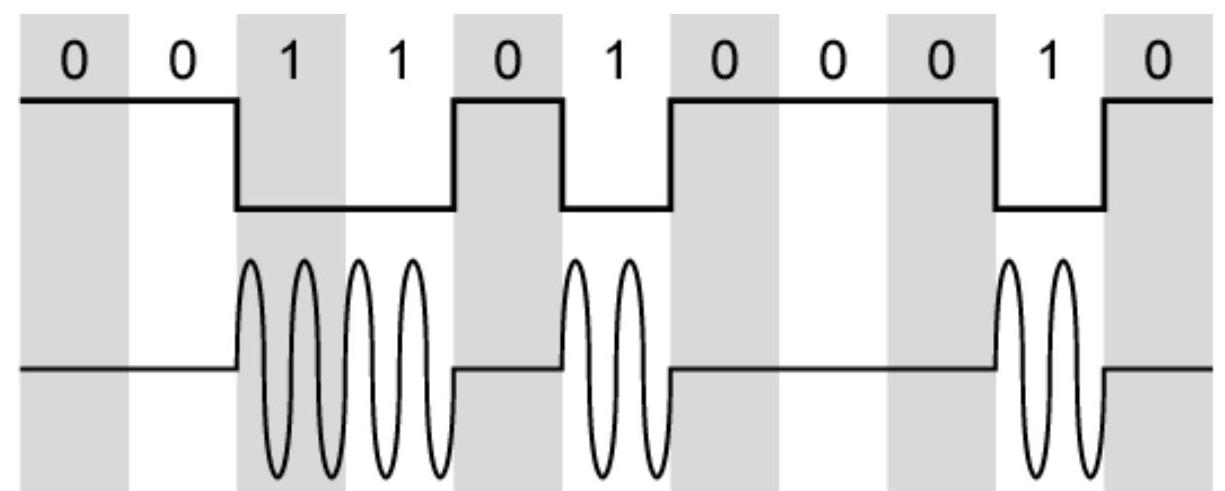
\includegraphics[max width=\textwidth]{2023_01_13_b07e3b4bcffdaab9792bg-068}
\end{center}

(b) BFSK

\begin{center}
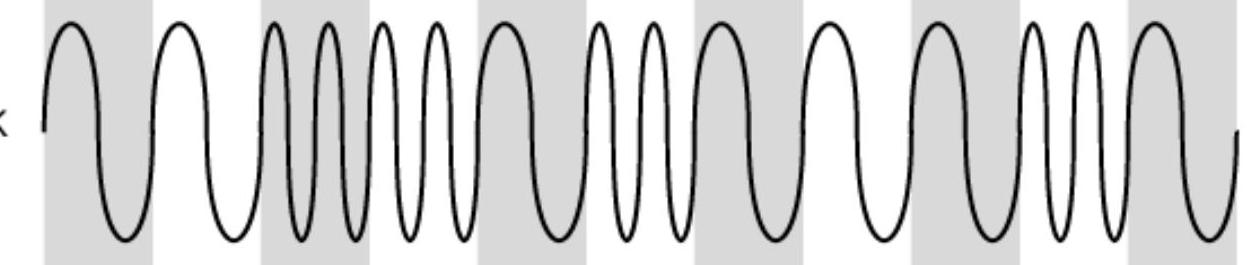
\includegraphics[max width=\textwidth]{2023_01_13_b07e3b4bcffdaab9792bg-068(1)}
\end{center}

(c) BPSK

\begin{center}
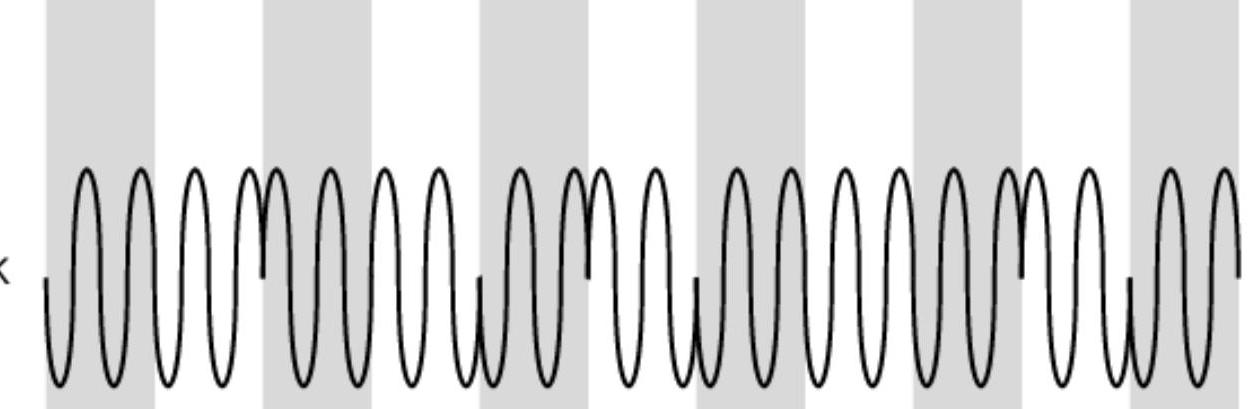
\includegraphics[max width=\textwidth]{2023_01_13_b07e3b4bcffdaab9792bg-068(2)}
\end{center}

\section{Amplitude Shift Keying}
\begin{itemize}
  \item Values represented by different amplitudes of carrier

  \item Usually, one amplitude is zero

\end{itemize}

o i.e. presence and absence of carrier is used

\begin{itemize}
  \item Susceptible to sudden gain changes

  \item Inefficient

  \item Up to 120obps on voice grade lines

  \item Used over optical fiber

\end{itemize}

\section{Binary Frequency Shift Keying}
\begin{itemize}
  \item Most common form is binary FSK (BFSK)

  \item Two binary values represented by two different frequencies (near carrier)

  \item Less susceptible to error than ASK

  \item Up to 120obps on voice grade lines

  \item High frequency radio

  \item Even higher frequency on LANs using co-ax

\end{itemize}

\section{Multiple FSK}
\begin{itemize}
  \item More than two frequencies used

  \item More bandwidth efficient

  \item More prone to error

  \item Each signalling element represents more than one bit

\end{itemize}

\section{FSK on Voice Grade Line}
signal strength

\begin{center}
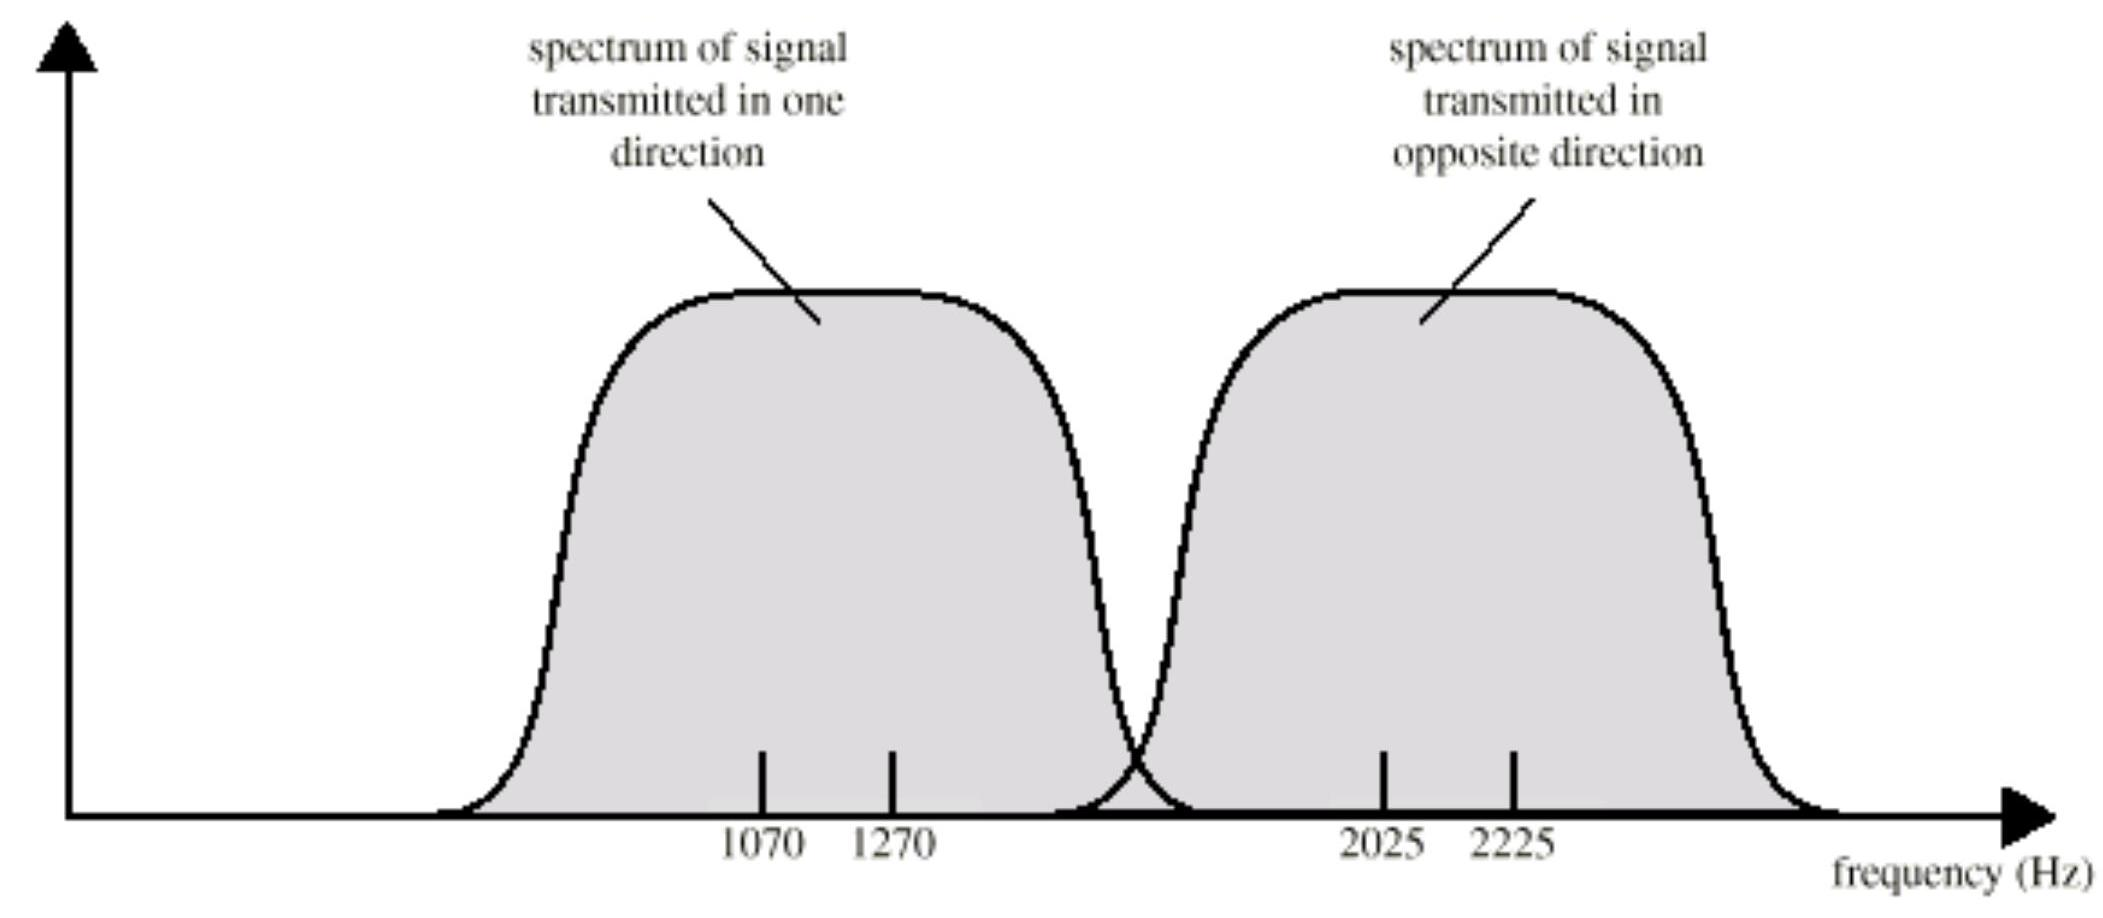
\includegraphics[max width=\textwidth]{2023_01_13_b07e3b4bcffdaab9792bg-072}
\end{center}

Figure 5.8 Full-Duplex FSK Transmission on a Voice-Grade Line

\section{Phase Shift Keying}
\begin{itemize}
  \item Phase of carrier signal is shifted to represent data - Binary PSK
\end{itemize}

o Two phases represent two binary digits

\begin{itemize}
  \item Differential PSK
\end{itemize}

o Phase shifted relative to previous transmission rather than some reference signal

\section{Differential PSK}
\begin{center}
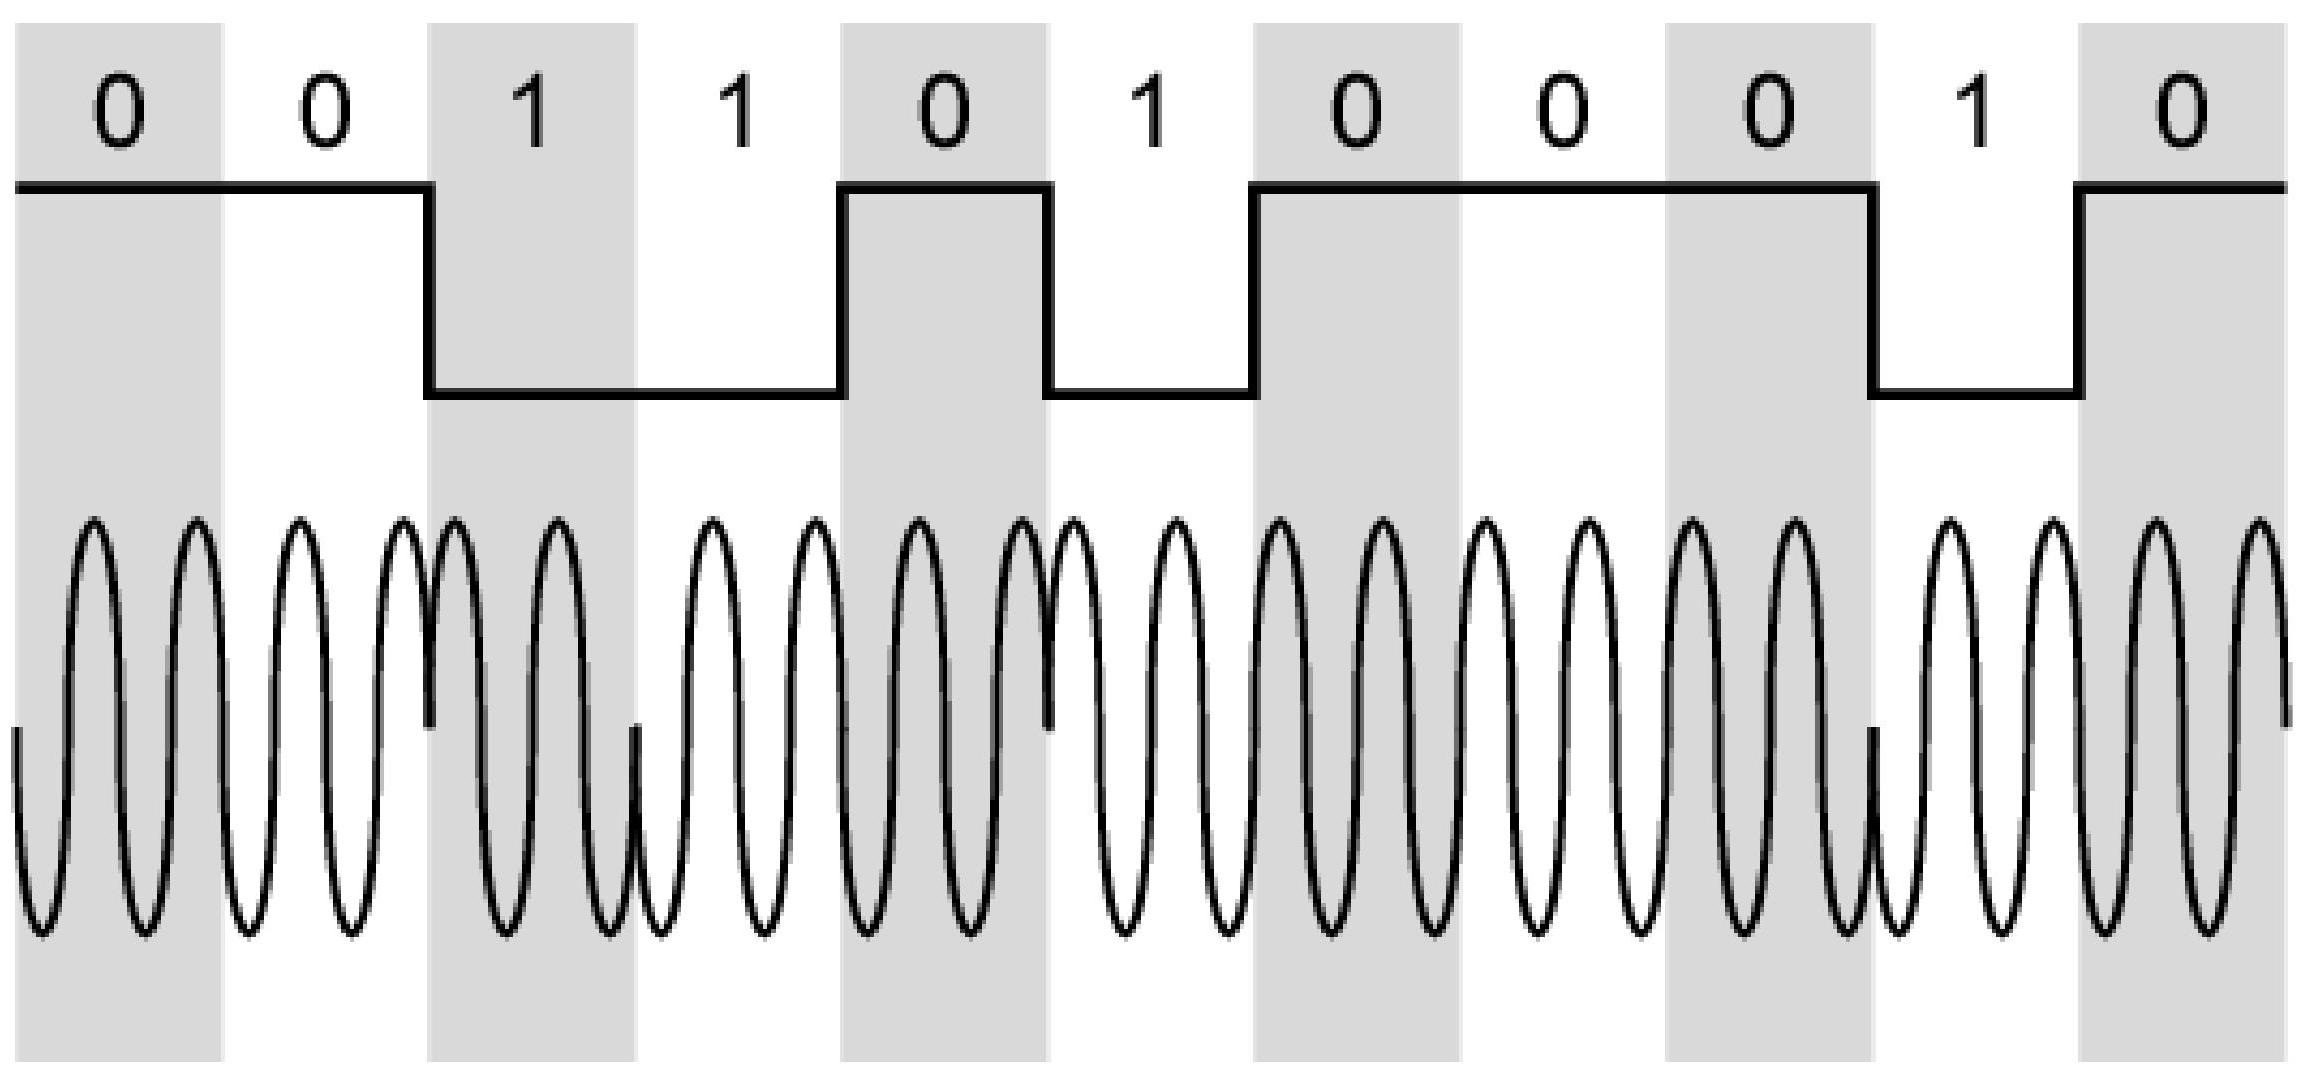
\includegraphics[max width=\textwidth]{2023_01_13_b07e3b4bcffdaab9792bg-074}
\end{center}

\section{Quadrature PSK}
\section{- More efficient use by each signal element representing more than one bit}
o e.g. shifts of $\pi / 2\left(90^{\circ}\right)$

o Each element represents two bits

o Can use 8 phase angles and have more than one amplitude o $9600 b p s$ modem use 12 angles, four of which have two amplitudes

\begin{itemize}
  \item Offset QPSK (orthogonal QPSK)
\end{itemize}

o Delay in Q stream

\section{QPSK and OQPSK Modulators}
$\mathrm{I}(\mathrm{t})$

R/2 bps

\begin{center}
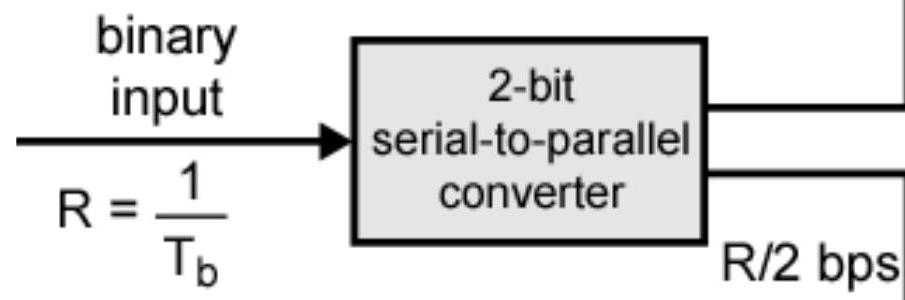
\includegraphics[max width=\textwidth]{2023_01_13_b07e3b4bcffdaab9792bg-076}
\end{center}

$a_{n}=\pm 1$

\begin{center}
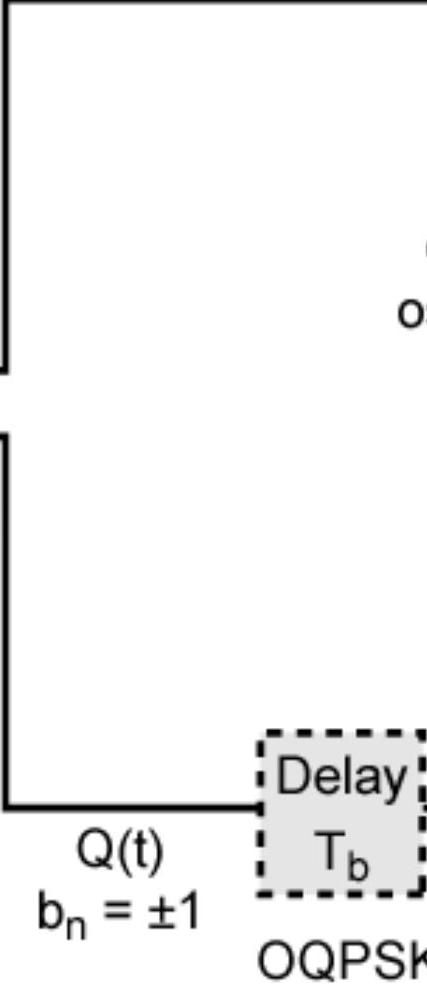
\includegraphics[max width=\textwidth]{2023_01_13_b07e3b4bcffdaab9792bg-076(1)}
\end{center}

only

\begin{center}
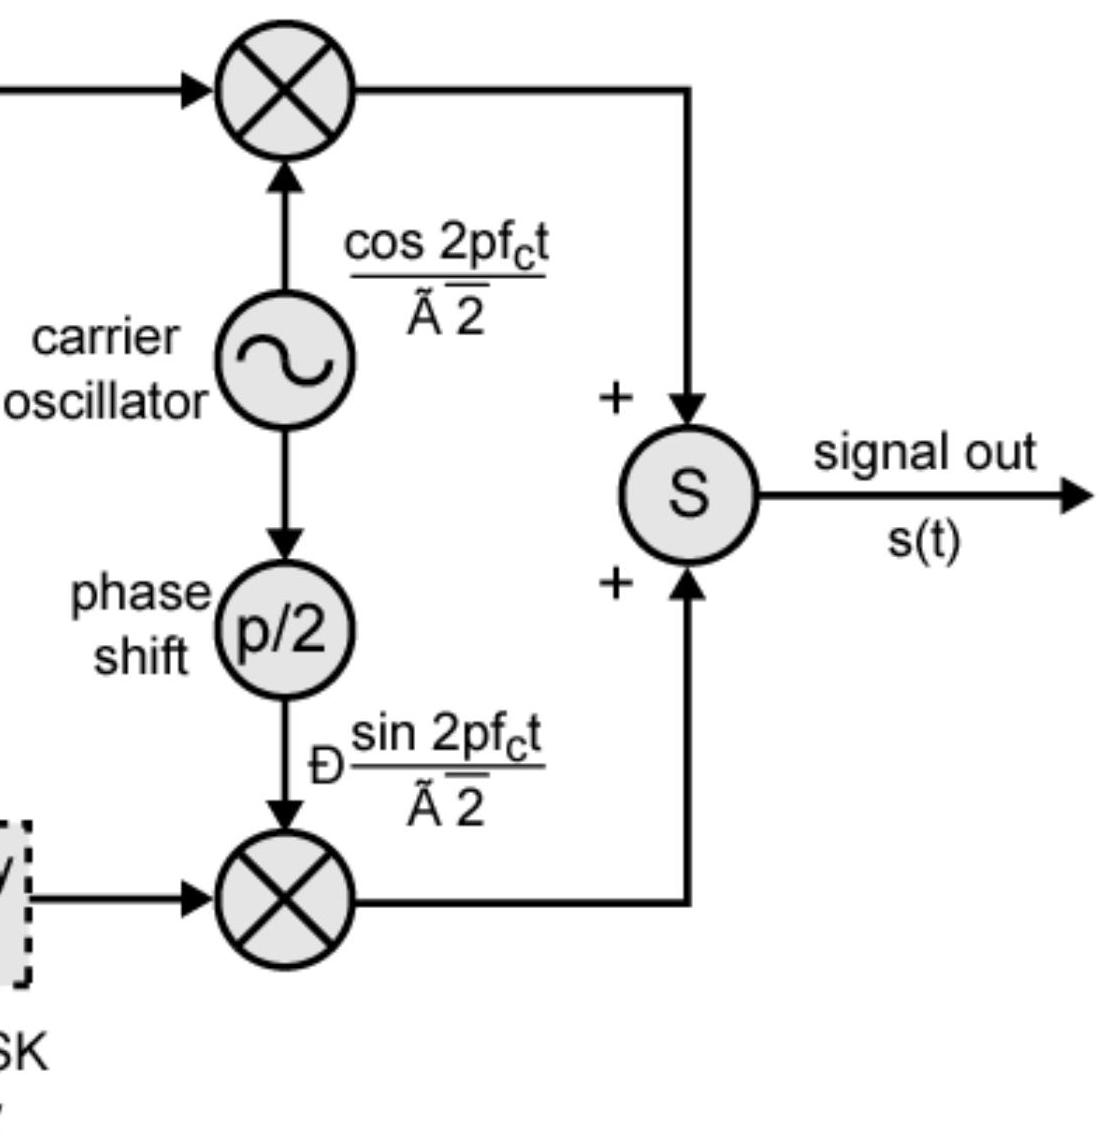
\includegraphics[max width=\textwidth]{2023_01_13_b07e3b4bcffdaab9792bg-076(2)}
\end{center}

\section{Examples of QPSF and OQPSK Waveforms}
\begin{center}
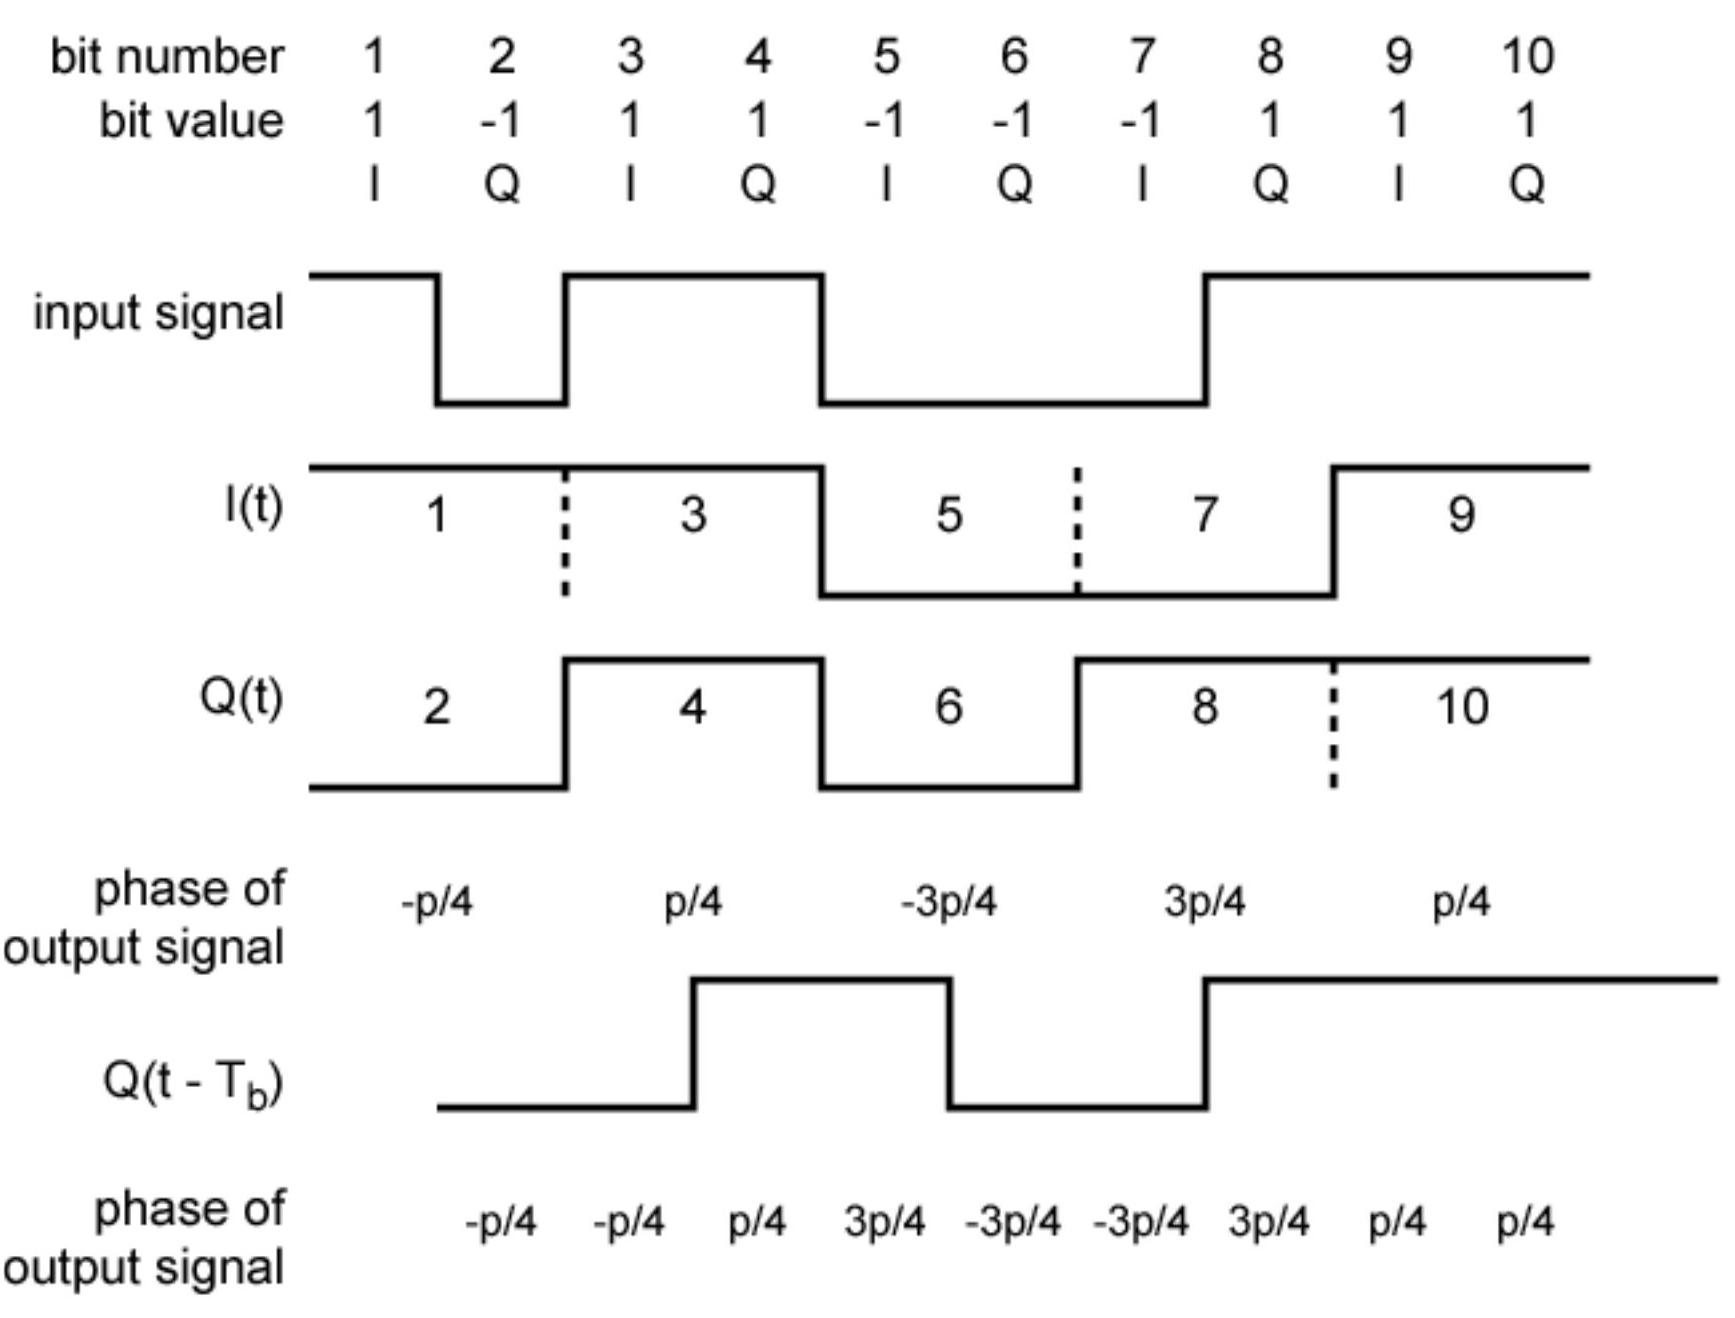
\includegraphics[max width=\textwidth]{2023_01_13_b07e3b4bcffdaab9792bg-077}
\end{center}

\section{Performance of Digital to Analog Modulation Schemes}
\begin{itemize}
  \item Bandwidth
\end{itemize}

ASK and PSK bandwidth directly related to bit rate

\begin{itemize}
  \item FSK bandwidth related to data rate for lower frequencies, but to offset of modulated frequency from carrier at high frequencies
\end{itemize}

o (See Stallings for math)

\begin{itemize}
  \item In the presence of noise, bit error rate of PSK and QPSK are about $3 \mathrm{~dB}$ superior to $\mathrm{ASK}$ and FSK
\end{itemize}

\section{Quadrature Amplitude Modulation}
\begin{itemize}
  \item QAM used on asymmetric digital subscriber line (ADSL) and some wireless

  \item Combination of ASK and PSK

  \item Logical extension of QPSK

  \item Send two different signals simultaneously on same carrier frequency

  \item Use two copies of carrier, one shifted $90^{\circ}$

\end{itemize}

o Each carrier is ASK modulated

o Two independent signals over same medium

\begin{itemize}
  \item Demodulate and combine for original binary output
\end{itemize}

\section{QAM Modulator}
\begin{center}
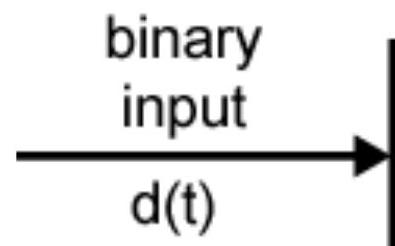
\includegraphics[max width=\textwidth]{2023_01_13_b07e3b4bcffdaab9792bg-080}
\end{center}

R bps

\begin{center}
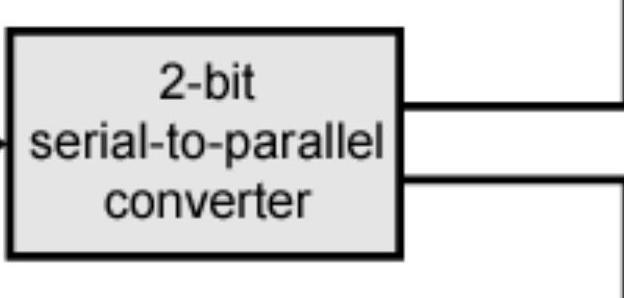
\includegraphics[max width=\textwidth]{2023_01_13_b07e3b4bcffdaab9792bg-080(1)}
\end{center}

$\mathrm{d}_{1}(\mathrm{t})$

R/2 bps

\begin{center}
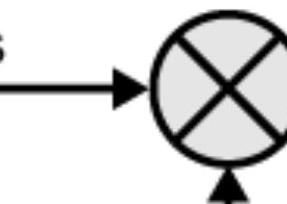
\includegraphics[max width=\textwidth]{2023_01_13_b07e3b4bcffdaab9792bg-080(2)}
\end{center}

$\int \cos 2 \mathrm{pf}_{\mathrm{c}} \mathrm{t}$
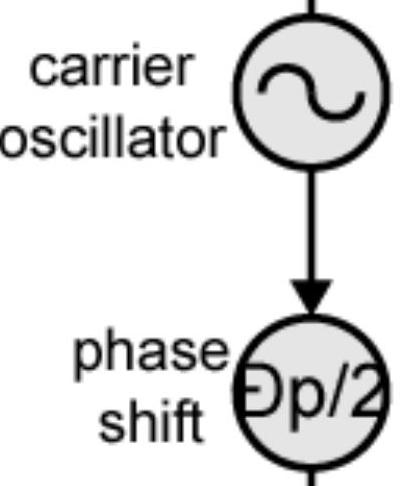
\includegraphics[max width=\textwidth, center]{2023_01_13_b07e3b4bcffdaab9792bg-080(3)}

QAM

signal out

$\begin{array}{r}d_{2}(t) \\ R / 2 \mathrm{bps} \\ \hline\end{array}$

$\begin{array}{r}\mathrm{d}_{2}(\mathrm{t}) \\ \mathrm{R} / 2 \mathrm{bps} \\ \hline\end{array}$

\begin{center}
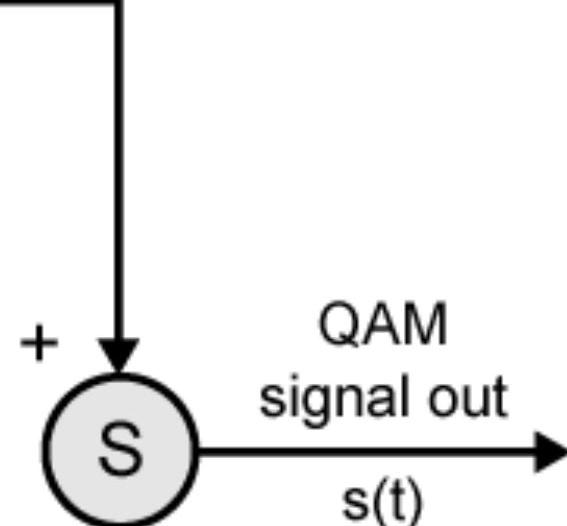
\includegraphics[max width=\textwidth]{2023_01_13_b07e3b4bcffdaab9792bg-080(4)}
\end{center}

\section{QAM Levels}
\begin{itemize}
  \item Two level ASK
\end{itemize}

o Each of two streams in one of two states

o Four state system

o Essentially QPSK

\begin{itemize}
  \item Four level ASK
\end{itemize}

o Combined stream in one of 16 states

\begin{itemize}
  \item 64 and 256 state systems have been implemented

  \item Improved data rate for given bandwidth

\end{itemize}

o Increased potential error rate

\section{Analog Data, Digital Signal}
\begin{itemize}
  \item Digitization

  \item Conversion of analog data into digital data

  \item Digital data can then be transmitted using NRZ-L

  \item Digital data can then be transmitted using code other than NRZ-L

  \item Digital data can then be converted to analog signal

  \item Analog to digital conversion done using a codec

  \item Pulse code modulation

\end{itemize}

o Delta modulation

\section{Digitizing Analog Data}
\begin{center}
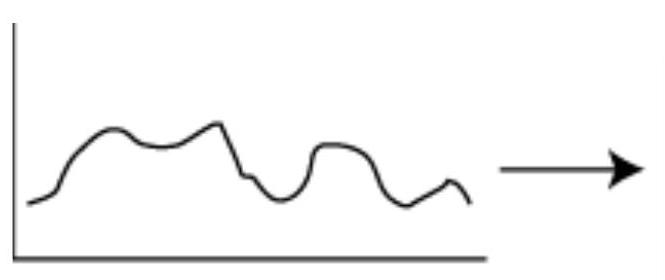
\includegraphics[max width=\textwidth]{2023_01_13_b07e3b4bcffdaab9792bg-083}
\end{center}

Analog data (voice)
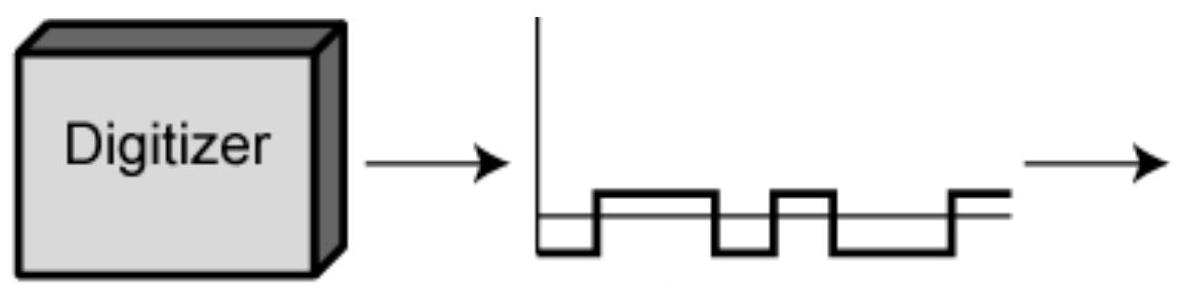
\includegraphics[max width=\textwidth, center]{2023_01_13_b07e3b4bcffdaab9792bg-083(1)}

Digital data

\begin{center}
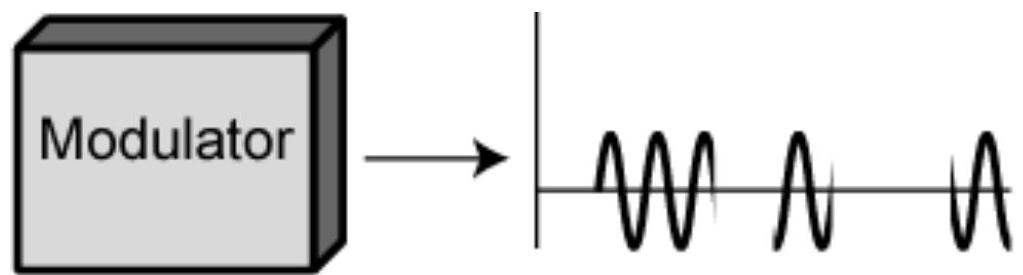
\includegraphics[max width=\textwidth]{2023_01_13_b07e3b4bcffdaab9792bg-083(2)}
\end{center}

Analog data

(ASK)

\section{Pulse Code Modulation(PCM) (1)}
\begin{itemize}
  \item If a signal is sampled at regular intervals at a rate higher than twice the highest signal frequency, the samples contain all the information of the original signal
\end{itemize}

o (Proof - Stallings appendix 4A)

\begin{itemize}
  \item Voice data limited to below $4000 \mathrm{~Hz}$

  \item Require 80oo sample per second

  \item Analog samples (Pulse Amplitude Modulation, PAM)

  \item Each sample assigned digital value

\end{itemize}

\section{Pulse Code Modulation(PCM) (2)}
\begin{itemize}
  \item 4 bit system gives 16 levels

  \item Quantized

\end{itemize}

o Quantizing error or noise

o Approximations mean it is impossible to recover original exactly

\begin{itemize}
  \item 8 bit sample gives 256 levels

  \item Quality comparable with analog transmission

  \item 8000 samples per second of 8 bits each gives $64 \mathrm{kbps}$

\end{itemize}

\section{PCM Example}
\begin{center}
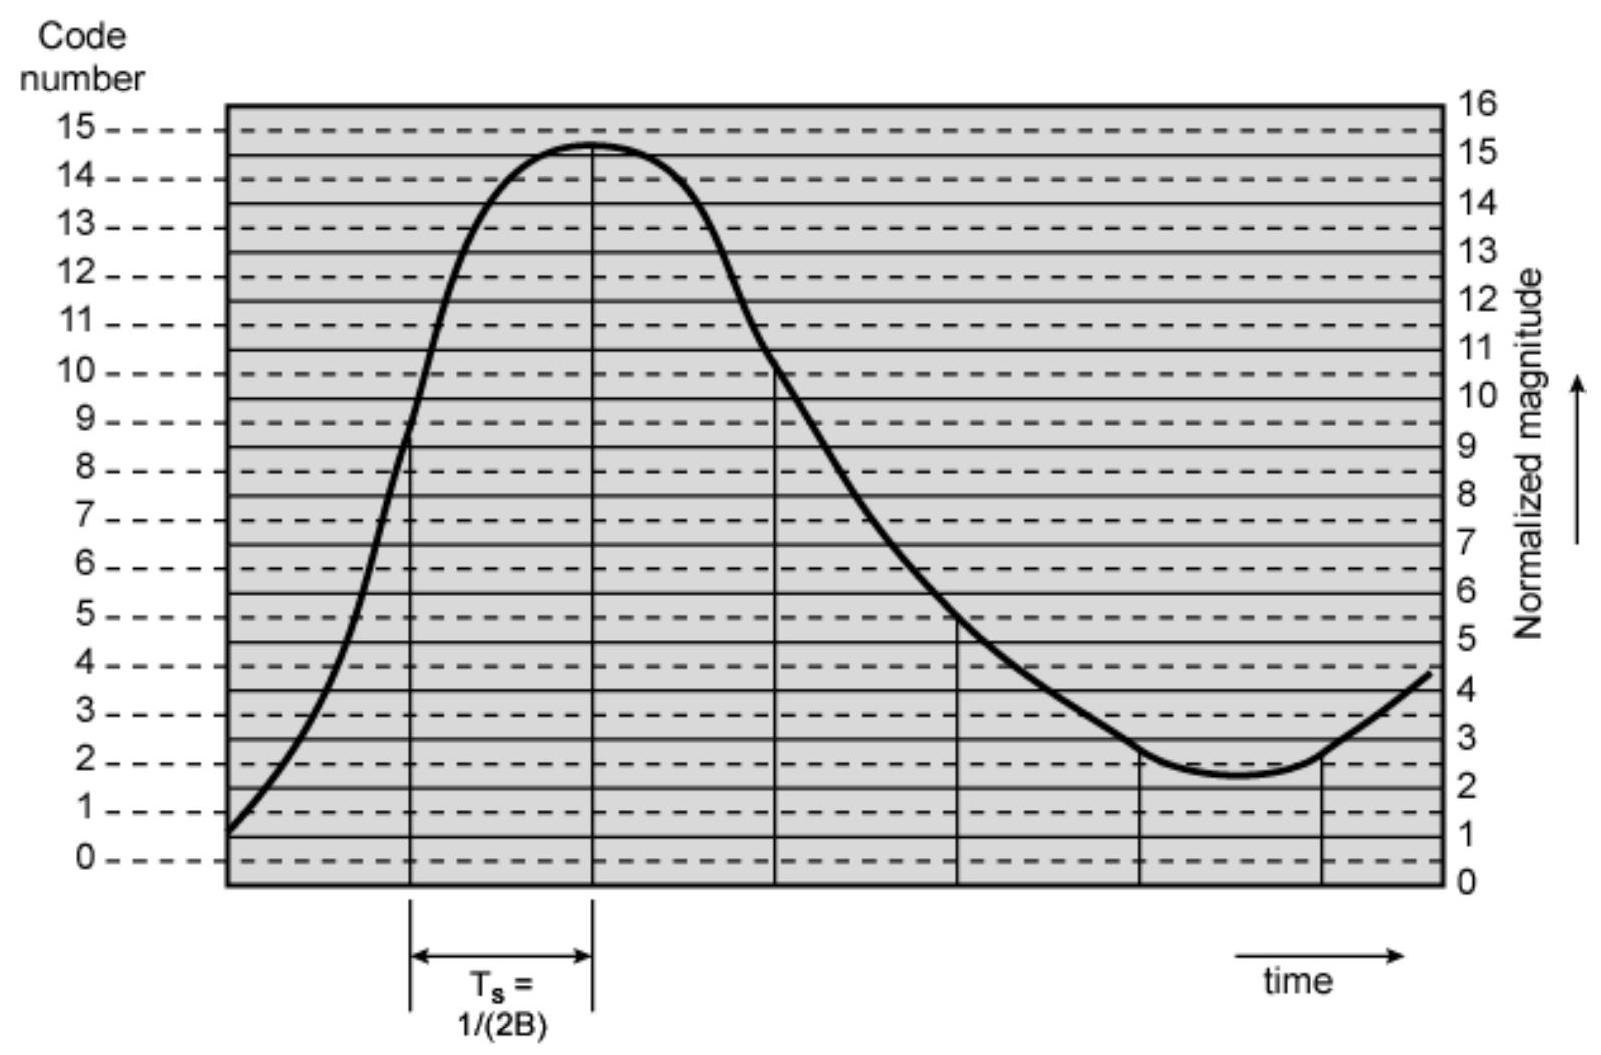
\includegraphics[max width=\textwidth]{2023_01_13_b07e3b4bcffdaab9792bg-086}
\end{center}

$\begin{array}{rccccccc}\text { PAM value } & 1.1 & 9.2 & 15.2 & 10.8 & 5.6 & 2.8 & 2.7 \\ \text { quantized code number } & 1 & 9 & 15 & 10 & 5 & 2 & 2 \\ \text { PCM code } & 0001 & 1001 & 1111 & 1010 & 0101 & 0010 & 0010\end{array}$

\section{PCM Block Diagram}
Continuous-time, continuous amplitud (analog) input signal

\begin{center}
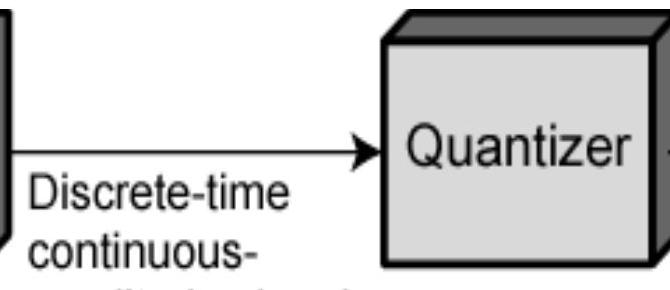
\includegraphics[max width=\textwidth]{2023_01_13_b07e3b4bcffdaab9792bg-087}
\end{center}

amplitude signal

(PAM pulses)

\begin{center}
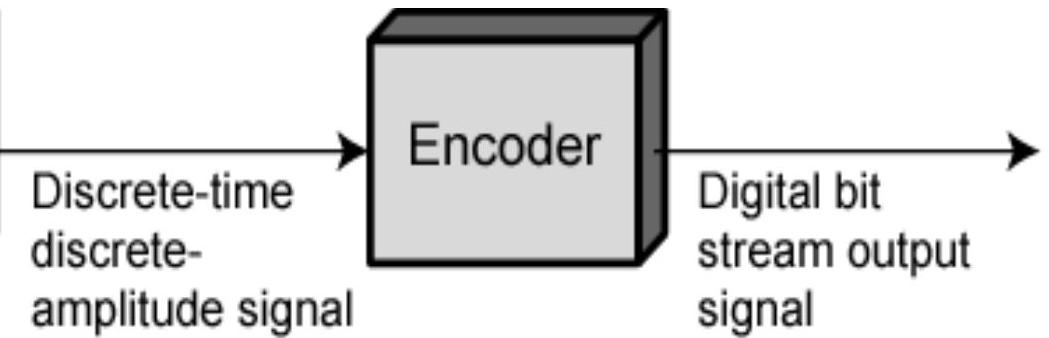
\includegraphics[max width=\textwidth]{2023_01_13_b07e3b4bcffdaab9792bg-087(1)}
\end{center}

(PCM pulses)

\section{Nonlinear Encoding}
\begin{itemize}
  \item Quantization levels not evenly spaced

  \item Reduces overall signal distortion

  \item Can also be done by companding

\end{itemize}

\section{Effect of Non-Linear Coding}
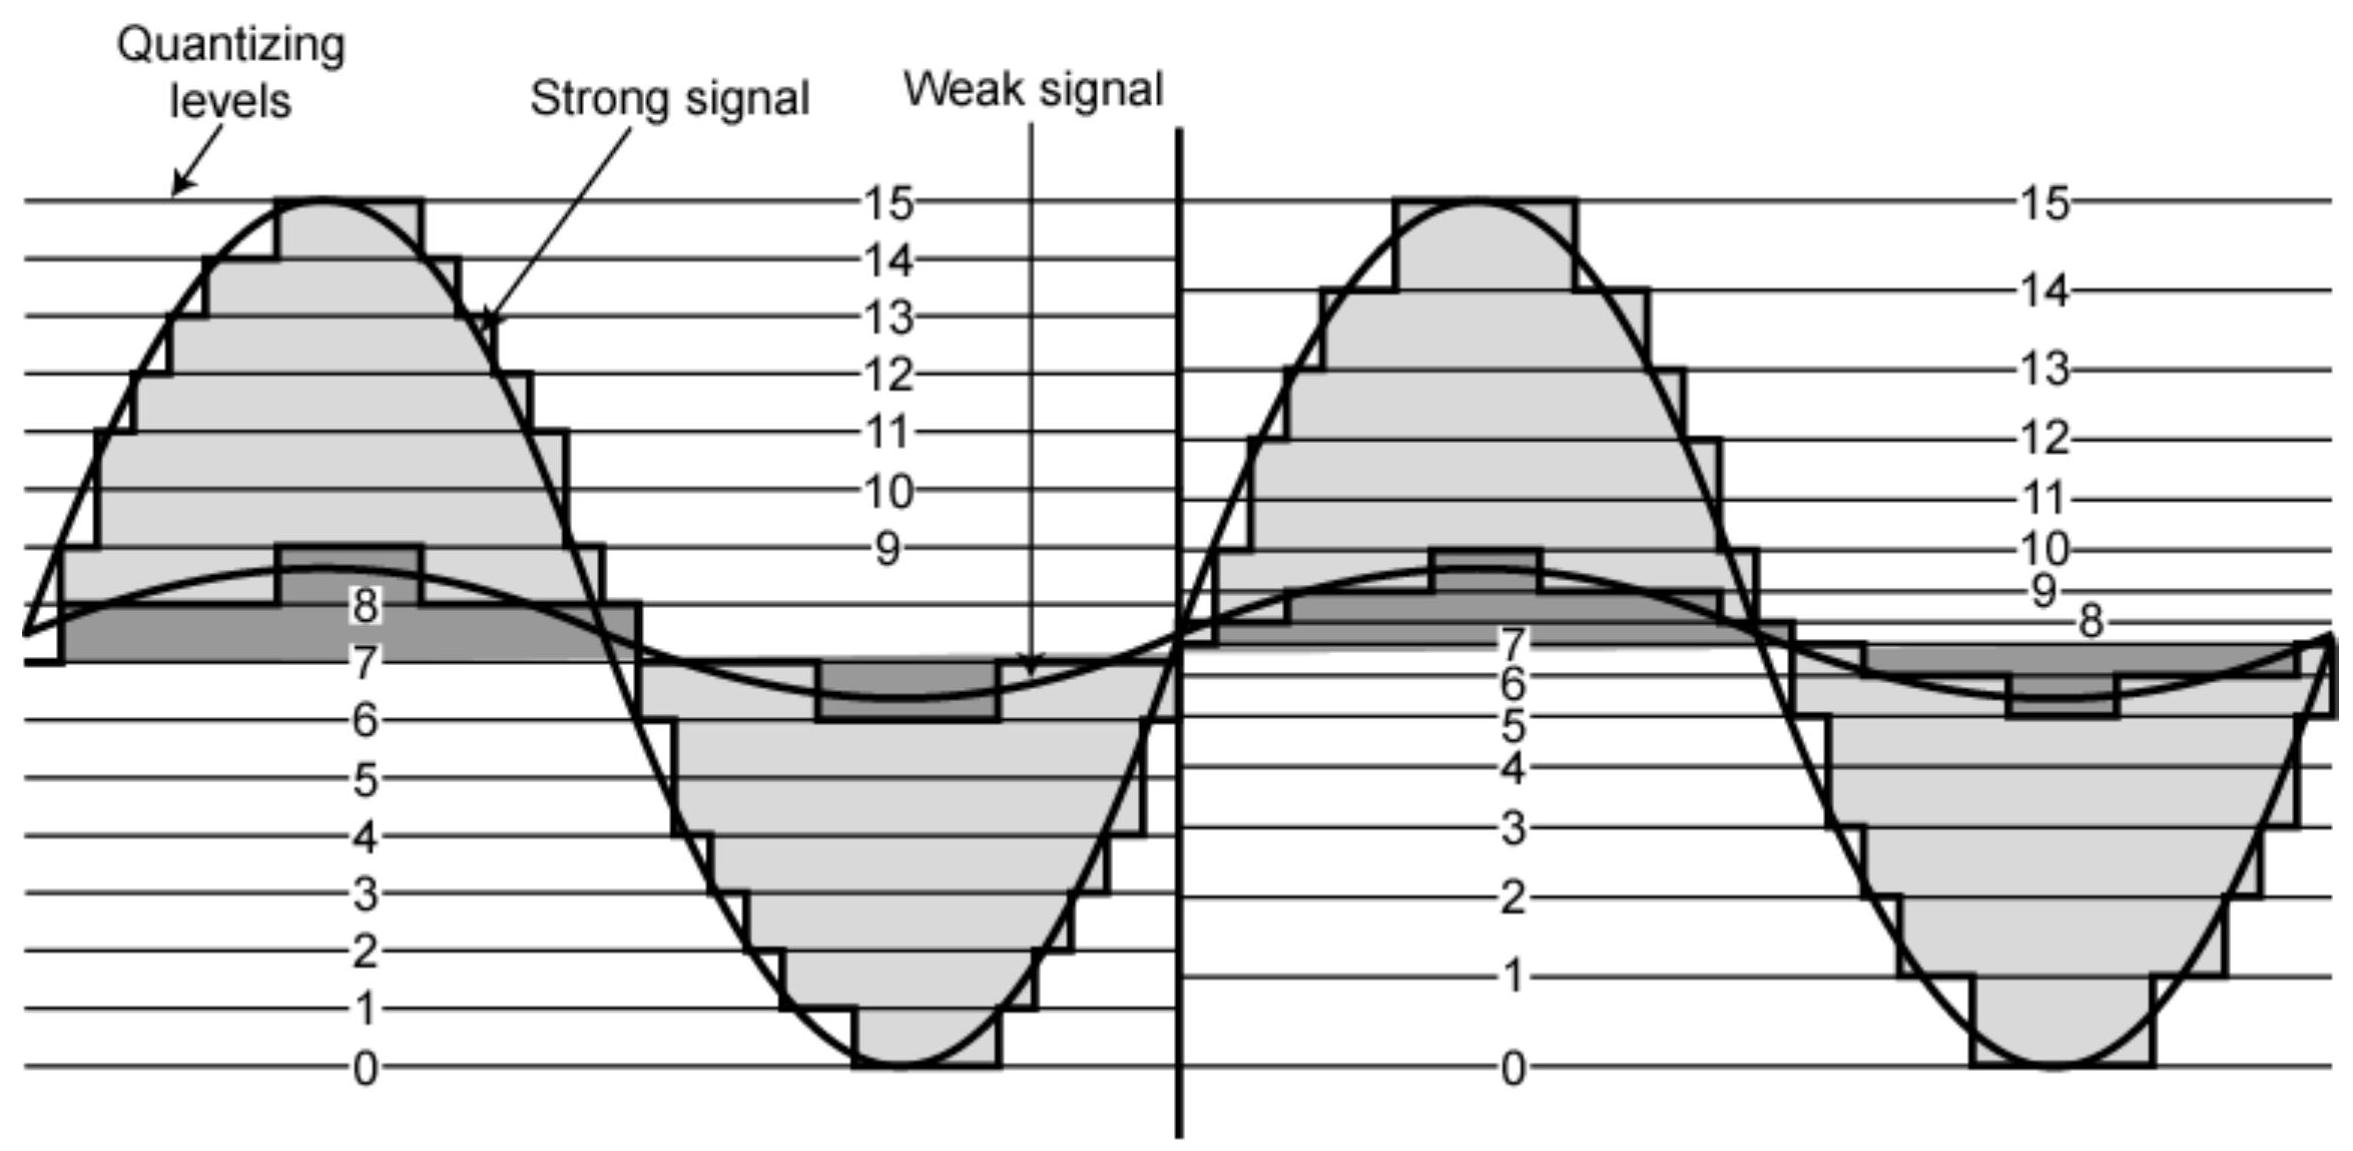
\includegraphics[max width=\textwidth, center]{2023_01_13_b07e3b4bcffdaab9792bg-089}
(a) Without nonlinear encoding
(b) With nonlinear encoding

\section{Typical Companding Functions}
\begin{center}
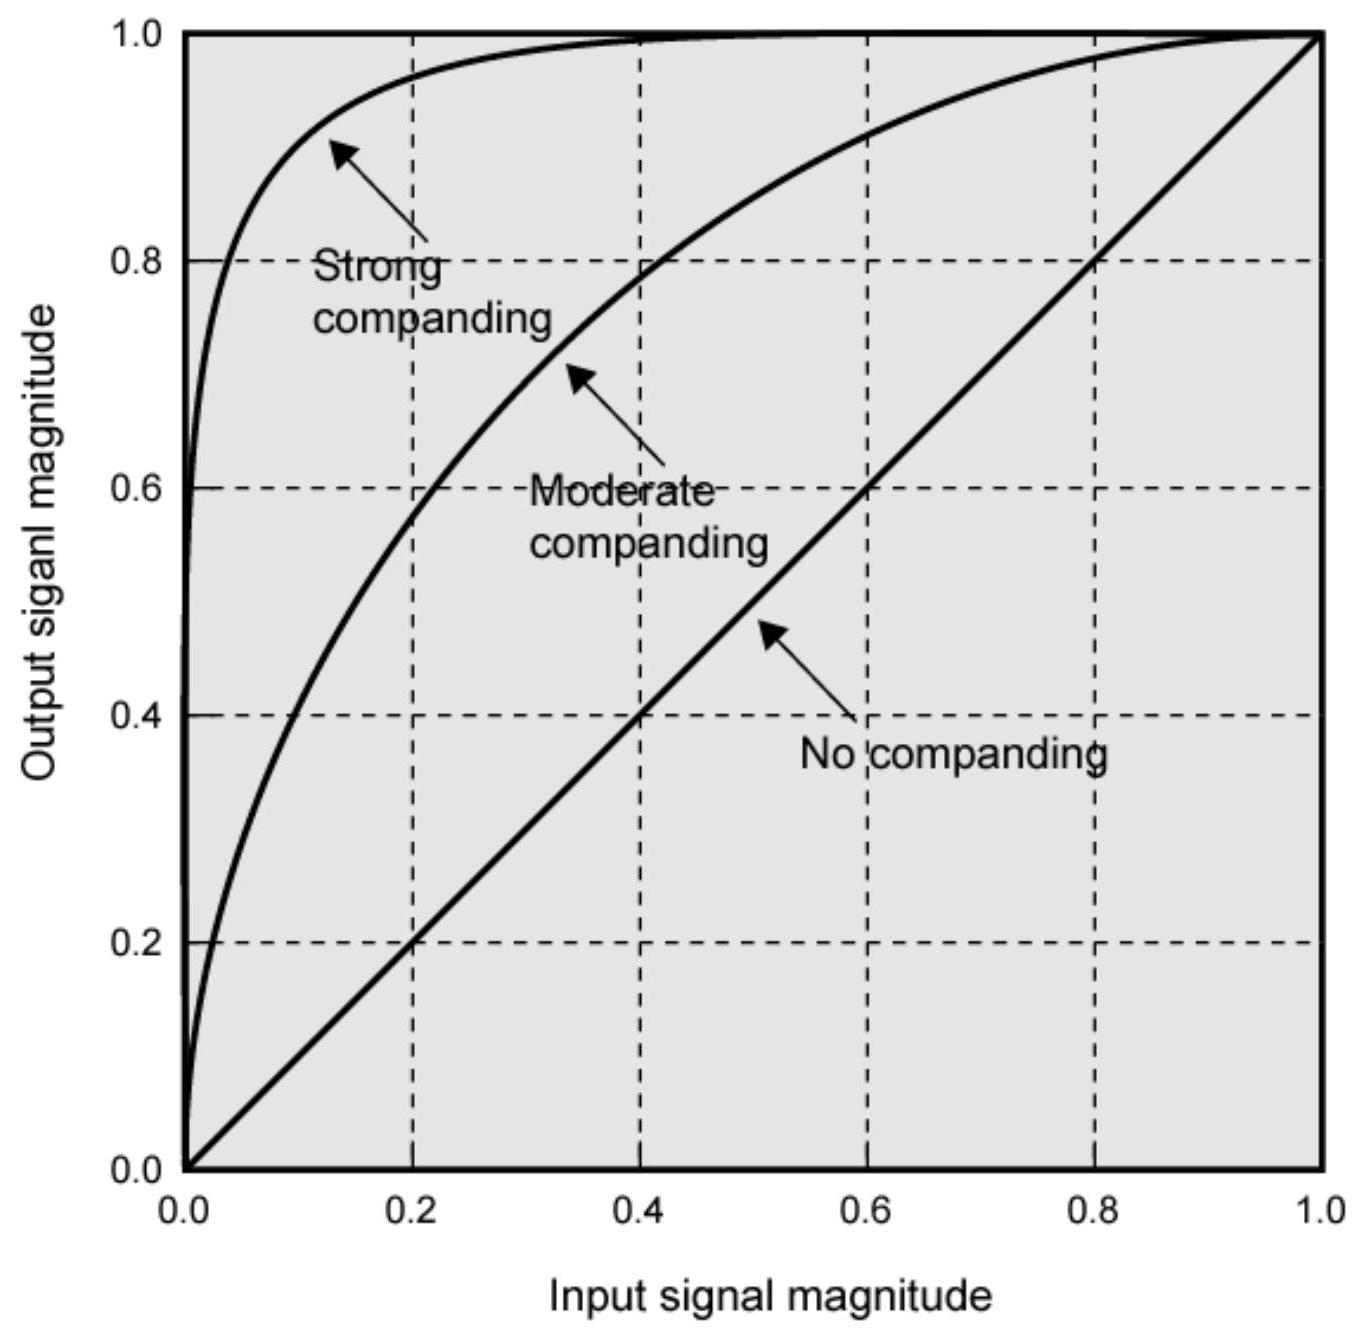
\includegraphics[max width=\textwidth]{2023_01_13_b07e3b4bcffdaab9792bg-090}
\end{center}

\section{Delta Modulation}
\begin{itemize}
  \item Analog input is approximated by a staircase function

  \item Move up or down one level ( $\delta$ ) at each sample interval

  \item Binary behavior

  \item Function moves up or down at each sample interval

\end{itemize}

\section{Delta Modulation - example}
\begin{center}
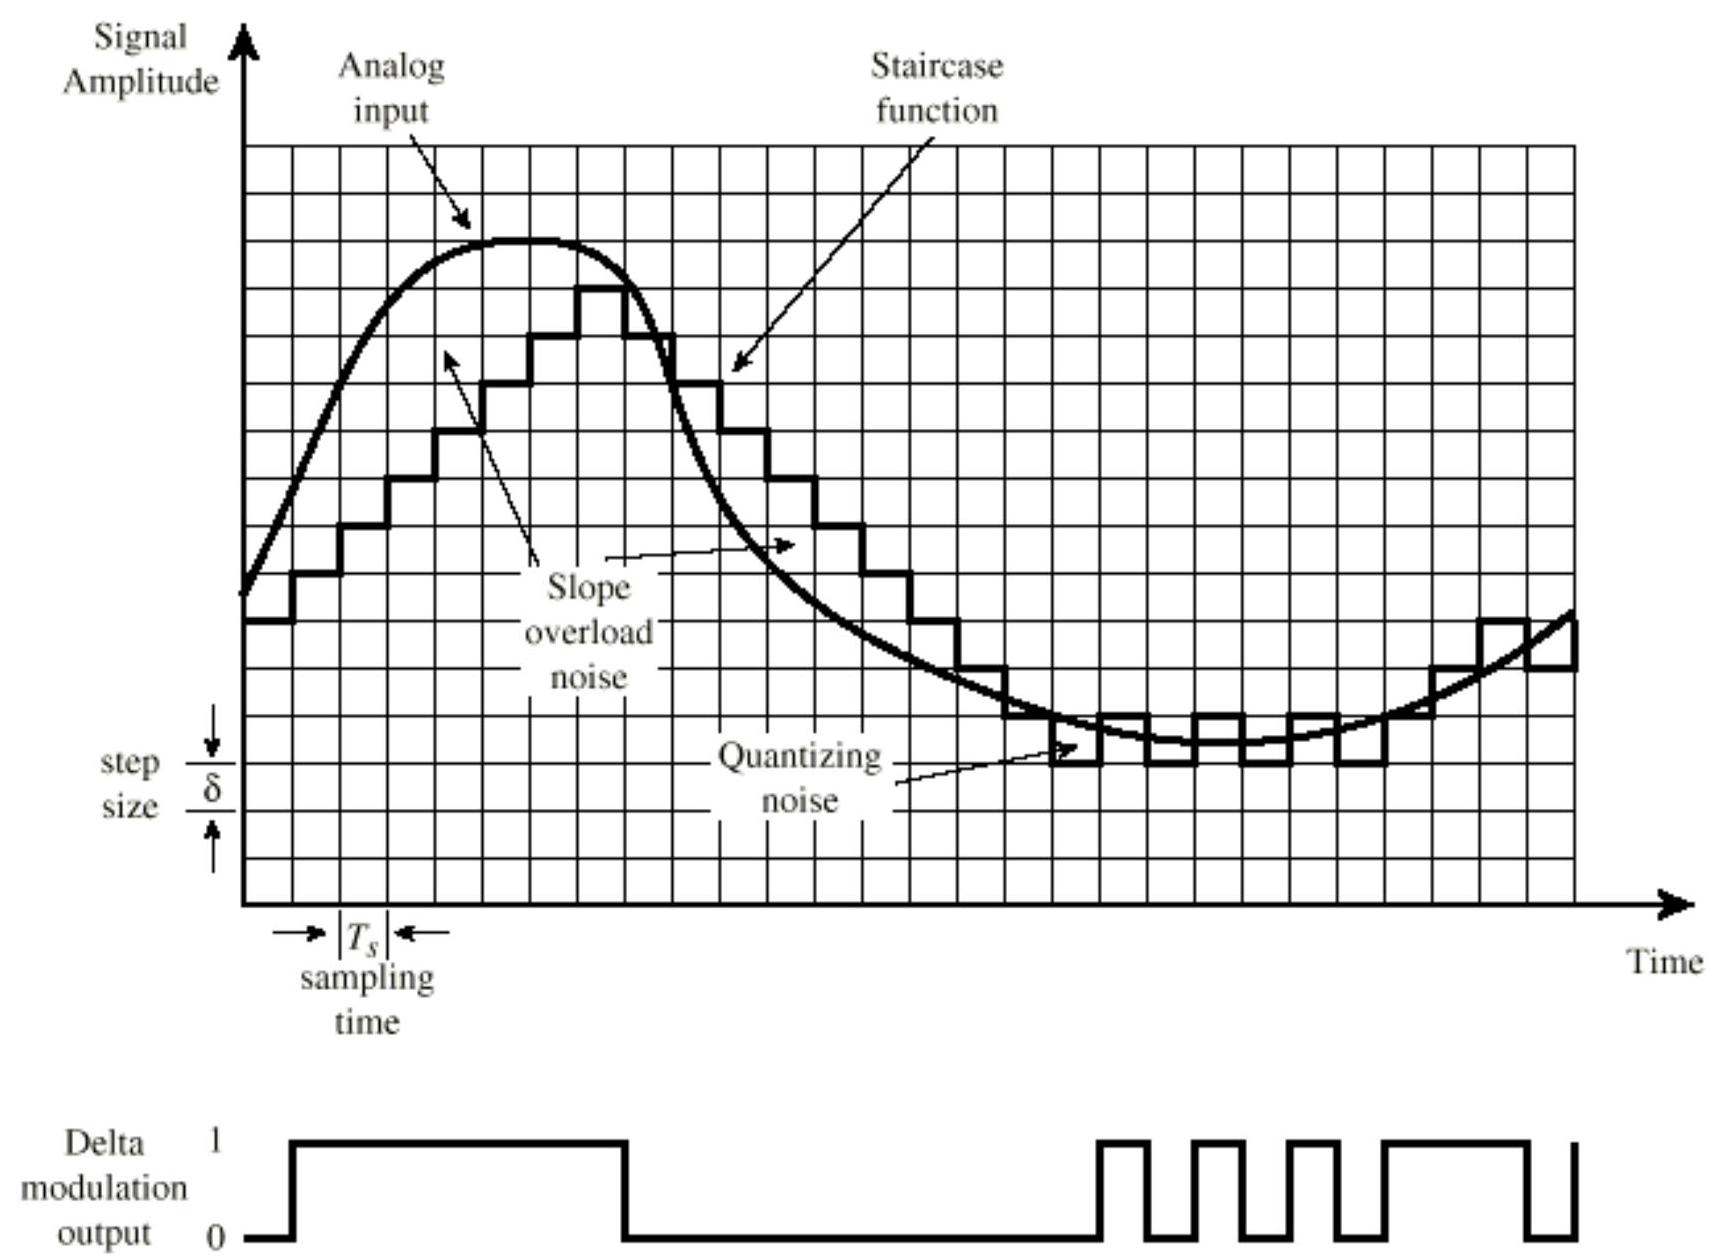
\includegraphics[max width=\textwidth]{2023_01_13_b07e3b4bcffdaab9792bg-092}
\end{center}

\section{Delta Modulation - Operation}
\begin{center}
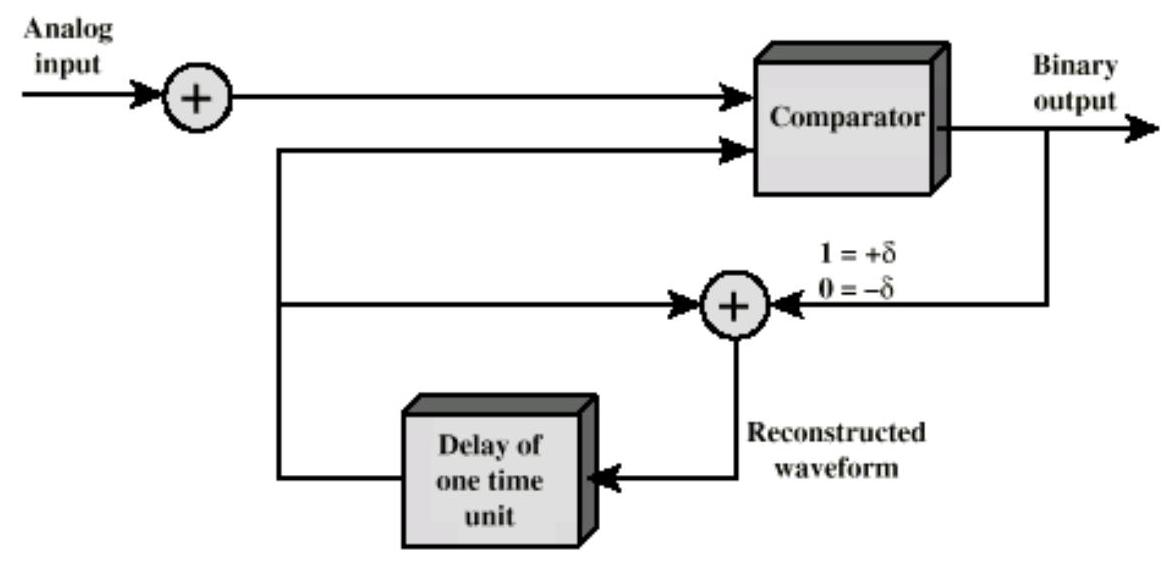
\includegraphics[max width=\textwidth]{2023_01_13_b07e3b4bcffdaab9792bg-093}
\end{center}

(a) Transmission

\begin{center}
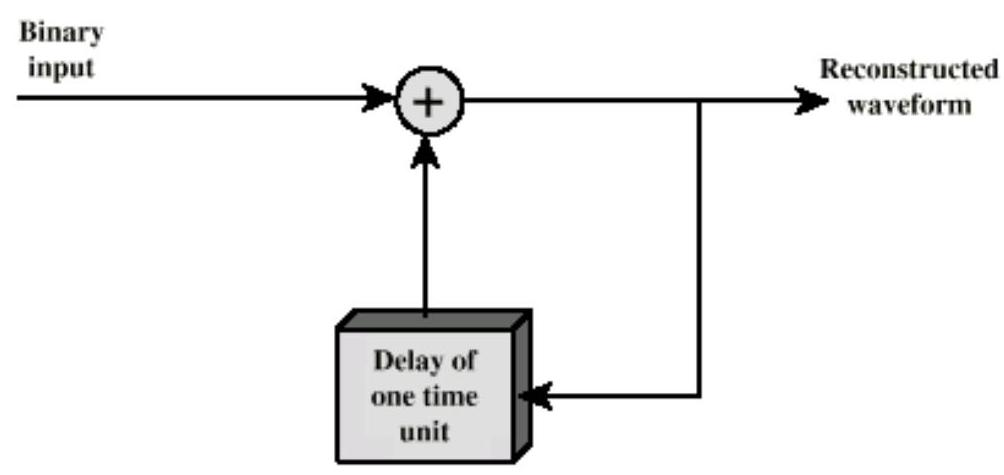
\includegraphics[max width=\textwidth]{2023_01_13_b07e3b4bcffdaab9792bg-093(1)}
\end{center}

(b) Reception

\section{Delta Modulation - Performance}
\begin{itemize}
  \item Good voice reproduction

  \item PCM - 128 levels (7 bit)

\end{itemize}

o Voice bandwidth $4 \mathrm{khz}$

o Should be $8000 \times 7=56 \mathrm{kbps}$ for PCM

\begin{itemize}
  \item Data compression can improve on this
\end{itemize}

o e.g. Interframe coding techniques for video

\section{Analog Data, Analog Signals}
\begin{itemize}
  \item Why modulate analog signals?

  \item Higher frequency can give more efficient transmission

  \item Permits frequency division multiplexing (chapter 8)

  \item Types of modulation

  \item Amplitude

  \item Frequency

\end{itemize}

o Phase

\section{Analog Modulation}
\begin{center}
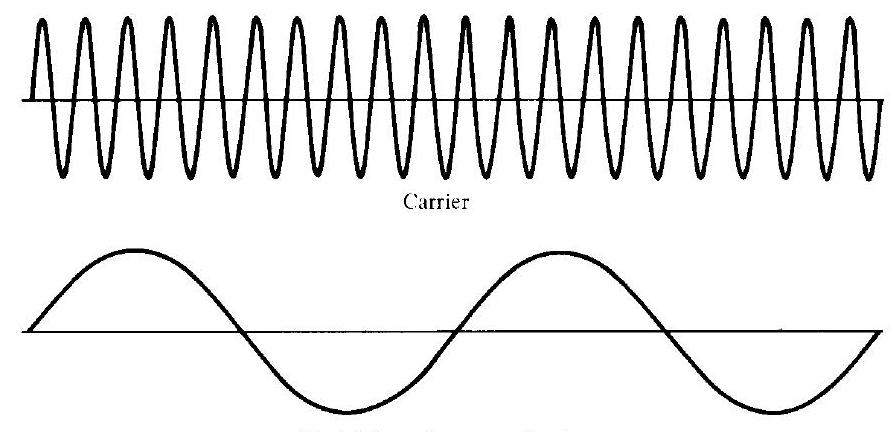
\includegraphics[max width=\textwidth]{2023_01_13_b07e3b4bcffdaab9792bg-096}
\end{center}

Modulating sine-wave signal

\begin{center}
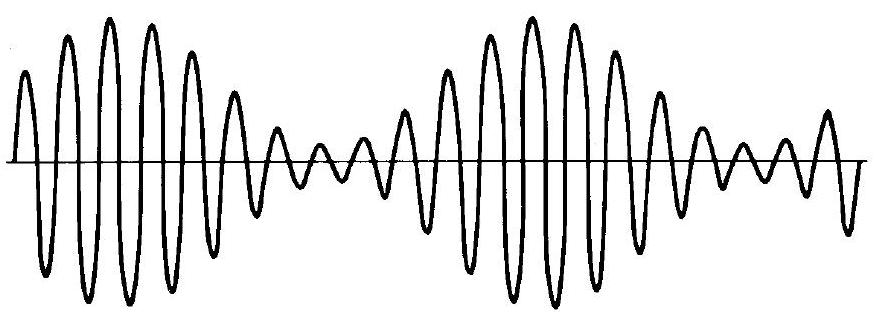
\includegraphics[max width=\textwidth]{2023_01_13_b07e3b4bcffdaab9792bg-096(1)}
\end{center}

Amplitude-modulated (DSBTC) wave

\begin{center}
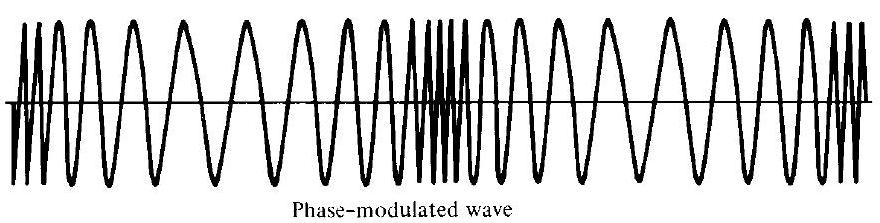
\includegraphics[max width=\textwidth]{2023_01_13_b07e3b4bcffdaab9792bg-096(2)}
\end{center}

Phase-modulated wave

\begin{center}
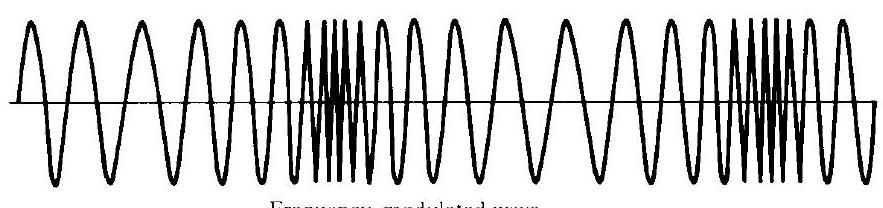
\includegraphics[max width=\textwidth]{2023_01_13_b07e3b4bcffdaab9792bg-096(3)}
\end{center}

\section{Ethernet}
\section{Ethernet}
\begin{itemize}
  \item Most successful local area networking technology of last 20 years.

  \item Developed in the mid-1970s by researchers at the Xerox Palo Alto Research Centers (PARC).

  \item Uses CSMA/CD technology

  \item Carrier Sense Multiple Access with Collision Detection.

  \item A set of nodes send and receive frames over a shared link.

  \item Carrier sense means that all nodes can distinguish between an idle and a busy link.

  \item Collision detection means that a node listens as it transmits and can therefore detect when a frame it is transmitting has collided with a frame transmitted by another node.

\end{itemize}

\section{Ethernet}
\begin{itemize}
  \item Uses ALOHA (packet radio network) as the root protocol

  \item Developed at the University of Hawaii to support communication across the Hawaiian Islands.

  \item For ALOHA the medium was atmosphere, for Ethernet the medium is a coax cable.

  \item DEC and Intel joined Xerox to define a 10-Mbps Ethernet standard in 1978.

  \item This standard formed the basis for IEEE standard 802.3

  \item More recently 802.3 has been extended to include a 100Mbps version called Fast Ethernet and a 1000-Mbps version called Gigabit Ethernet.

\end{itemize}

\section{Ethernet}
\begin{itemize}
  \item An Ethernet segment is implemented on a coaxial cable of up to $500 \mathrm{~m}$.

  \item This cable is similar to the type used for cable TV except that it typically has an impedance of 50 ohms instead of cable TV's 75 ohms.

  \item Hosts connect to an Ethernet segment by tapping into it.

  \item A transceiver (a small device directly attached to the tap) detects when the line is idle and drives signal when the host is transmitting.

  \item The transceiver also receives incoming signal.

  \item The transceiver is connected to an Ethernet adaptor which is plugged into the host.

  \item The protocol is implemented on the adaptor.

\end{itemize}

\section{Ethernet}
Transceiver

\begin{center}
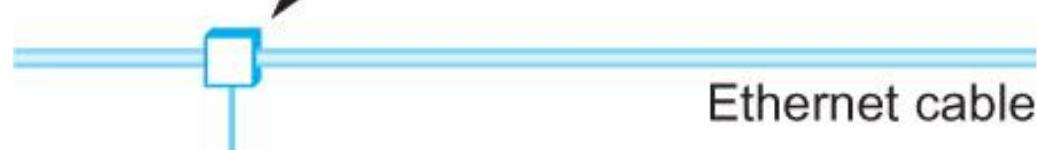
\includegraphics[max width=\textwidth]{2023_01_13_b07e3b4bcffdaab9792bg-101}
\end{center}

Adaptor

Host

\section{Ethernet transceiver and adaptor}
\section{Ethernet}
\begin{itemize}
  \item Multiple Ethernet segments can be joined together by repeaters.

  \item A repeater is a device that forwards digital signals.

  \item No more than four repeaters may be positioned between any pair of hosts.

\end{itemize}

o An Ethernet has a total reach of only $2500 \mathrm{~m}$.

\section{Ethernet - Repeater}
\begin{center}
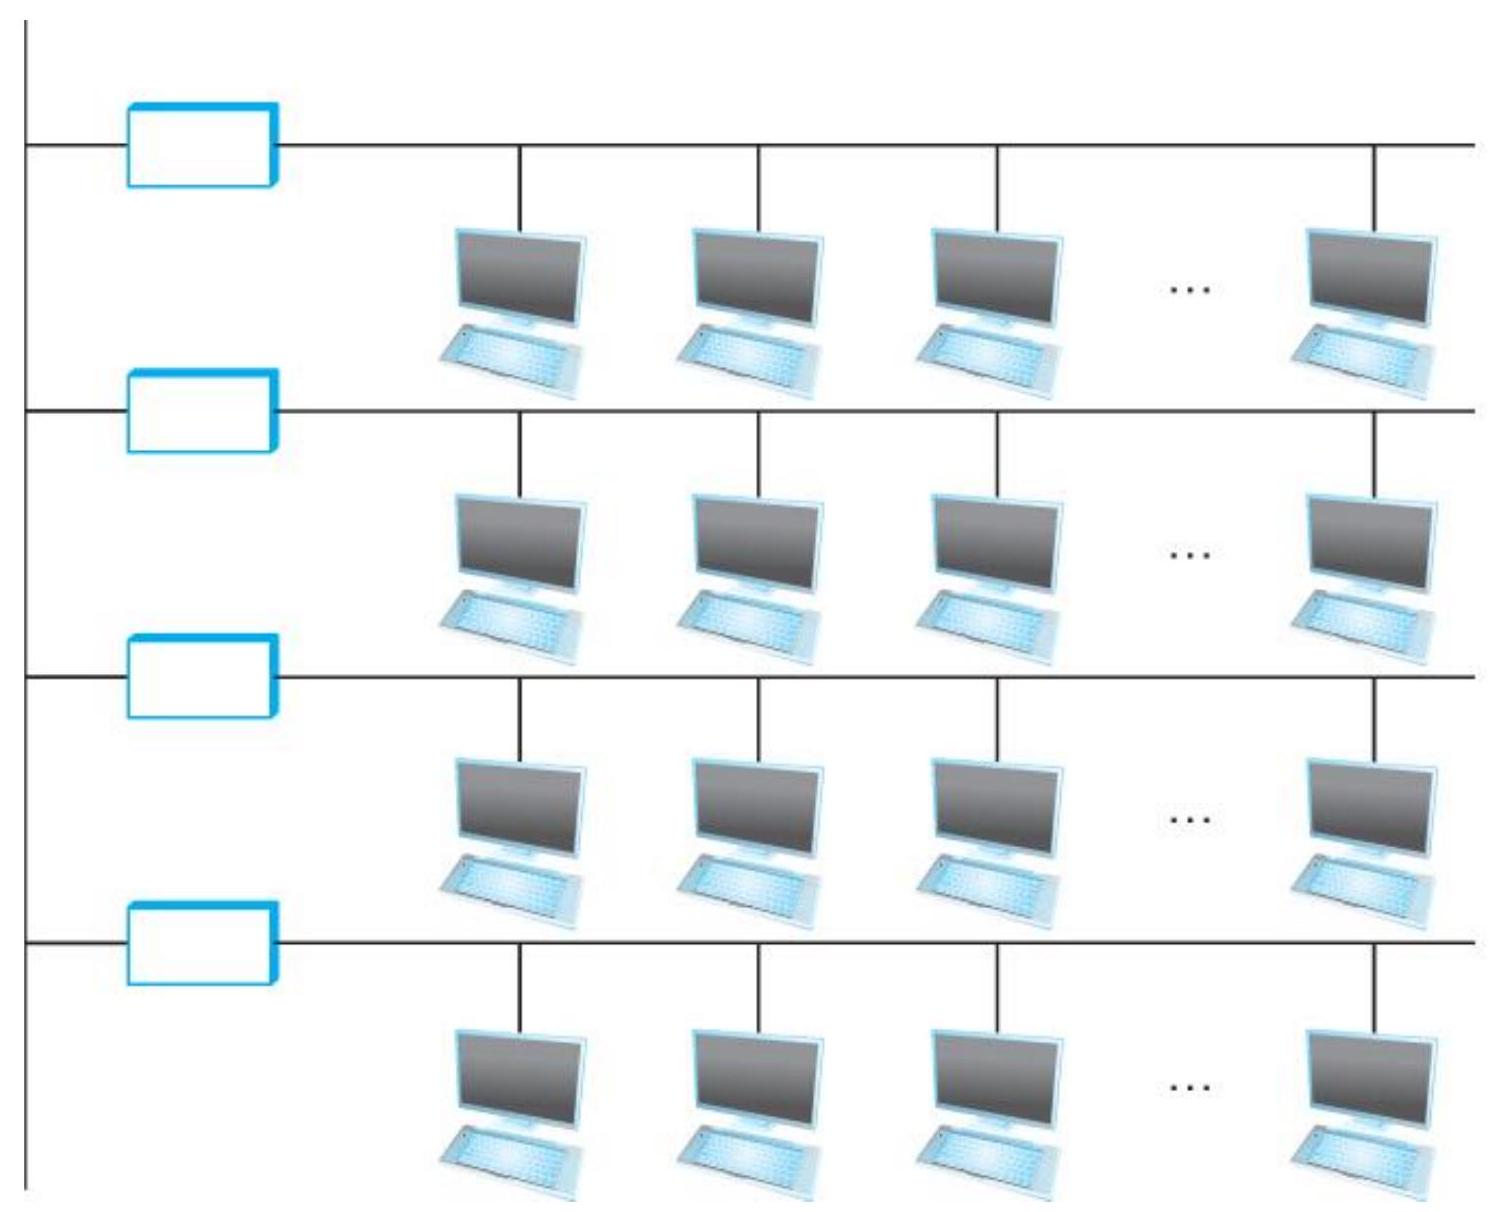
\includegraphics[max width=\textwidth]{2023_01_13_b07e3b4bcffdaab9792bg-103}
\end{center}

\begin{center}
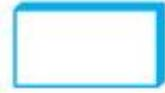
\includegraphics[max width=\textwidth]{2023_01_13_b07e3b4bcffdaab9792bg-103(1)}
\end{center}

Repeater

\begin{center}
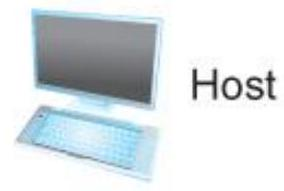
\includegraphics[max width=\textwidth]{2023_01_13_b07e3b4bcffdaab9792bg-103(2)}
\end{center}

\section{Ethernet}
\begin{itemize}
  \item Any signal placed on the Ethernet by a host is broadcast over the entire network
\end{itemize}

o Signal is propagated in both directions.

o Repeaters forward the signal on all outgoing segments.

o Terminators attached to the end of each segment absorb the signal.

\begin{itemize}
  \item Ethernet uses Manchester encoding scheme.
\end{itemize}

\section{Ethernet}
\begin{itemize}
  \item New Technologies in Ethernet

  \item Instead of using coax cable, an Ethernet can be constructed from a thinner cable known as 10 Base2 (the original was 10Base5)

\end{itemize}

10 means the network operates at $10 \mathrm{Mbps}$

· Base means the cable is used in a baseband system

$\times 2$ means that a given segment can be no longer than $200 \mathrm{~m}$

\section{Ethernet}
\begin{itemize}
  \item New Technologies in Ethernet - Another cable technology is 10BaseT
\end{itemize}

\begin{CJK}{UTF8}{mj}乂\end{CJK} T stands for twisted pair

\begin{itemize}
  \item Limited to $100 \mathrm{~m}$ in length
\end{itemize}

o With 10 BaseT, the common configuration is to have several point to point segments coming out of a multiway repeater, called $H u b$

\section{Ethernet}
\begin{center}
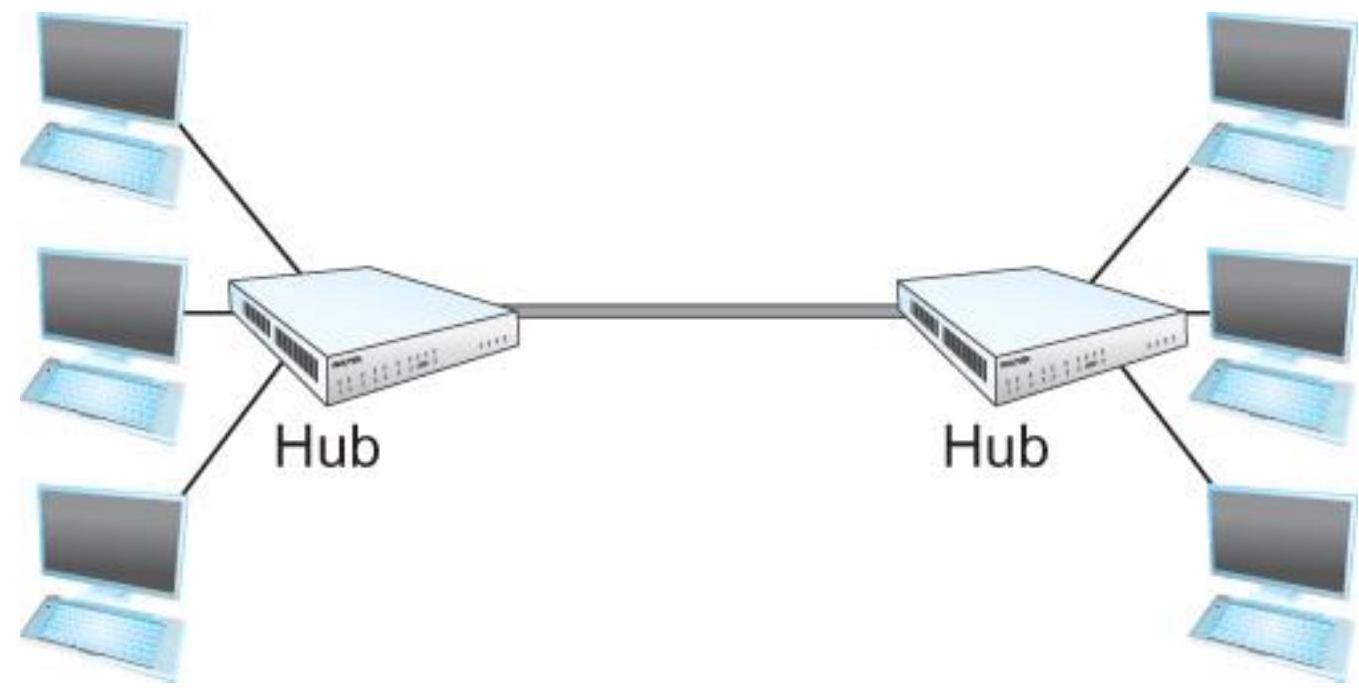
\includegraphics[max width=\textwidth]{2023_01_13_b07e3b4bcffdaab9792bg-107}
\end{center}

Ethernet Hub

\section{Access Protocol for Ethernet}
\begin{itemize}
  \item The algorithm is commonly called Ethernet's Media Access Control (MAC).
\end{itemize}

o It is implemented in Hardware on the network adaptor.

\begin{itemize}
  \item Frame format
\end{itemize}

o Preamble (64bit): allows the receiver to synchronize with the signal (sequence of alternating os and 1s).

o Host and Destination Address (48bit each).

o Packet type (16bit): acts as demux key to identify the higher level protocol.

o Data (up to 1500 bytes)

\begin{itemize}
  \item Minimally a frame must contain at least 46 bytes of data.

  \item Frame must be long enough to detect collision.

\end{itemize}

o CRC (32bit)

\section{Ethernet Frame}
\begin{center}
\begin{tabular}{|c|c|c|c|c|c|}
64 & 48 & 48 & 16 & 32 &  \\
\hline
Preamble & Dest addr & Src addr & Type & Body & CRC \\
\hline
\end{tabular}
\end{center}

\section{Ethernet Frame Format}
\section{Ethernet Addresses}
\begin{itemize}
  \item Each host on an Ethernet (in fact, every Ethernet host in the world) has a unique Ethernet Address.

  \item The address belongs to the adaptor, not the host.

\end{itemize}

o It is usually burnt into ROM.

\begin{itemize}
  \item Ethernet addresses are typically printed in a human readable format
\end{itemize}

o As a sequence of six numbers separated by colons.

o Each number corresponds to 1 byte of the 6 byte address and is given by a pair of hexadecimal digits, one for each of the 4-bit nibbles in the byte

o Leading os are dropped.

o For example, 8:0:2b:e4:b1:2 is

· 000010000000000000101011111001001011000100000010

\section{Ethernet Addresses}
\begin{itemize}
  \item To ensure that every adaptor gets a unique address, each manufacturer of Ethernet devices is allocated a different prefix that must be prepended to the address on every adaptor they build
\end{itemize}

\begin{itemize}
  \item AMD has been assigned the 24bit prefix 8:0:20
\end{itemize}

\section{Ethernet Addresses}
\begin{itemize}
  \item Each frame transmitted on an Ethernet is received by every adaptor connected to that Ethernet.

  \item Each adaptor recognizes those frames addressed to its address and passes only those frames on to the host.

  \item In addition, to unicast address, an Ethernet address consisting of all $1 \mathrm{~s}$ is treated as a broadcast address.

\end{itemize}

o All adaptors pass frames addressed to the broadcast address up to the host.

\begin{itemize}
  \item Similarly, an address that has the first bit set to 1 but is not the broadcast address is called a multicast address.
\end{itemize}

o A given host can program its adaptor to accept some set of multicast addresses.

\section{Ethernet Addresses}
\begin{itemize}
  \item To summarize, an Ethernet adaptor receives all frames and accepts
\end{itemize}

o Frames addressed to its own address

o Frames addressed to the broadcast address

o Frames addressed to a multicast addressed if it has been instructed

\section{Ethernet Transmitter Algorithm}
\begin{itemize}
  \item When the adaptor has a frame to send and the line is idle, it transmits the frame immediately.

  \item The upper bound of 1500 bytes in the message means that the adaptor can occupy the line for a fixed length of time.

  \item When the adaptor has a frame to send and the line is busy, it waits for the line to go idle and then transmits immediately.

  \item The Ethernet is said to be 1-persistent protocol because an adaptor with a frame to send transmits with probability 1 whenever a busy line goes idle.

\end{itemize}

\section{Ethernet Transmitter Algorithm}
\begin{itemize}
  \item Since there is no centralized control it is possible for two (or more) adaptors to begin transmitting at the same time,

  \item Either because both found the line to be idle,

  \item Or, both had been waiting for a busy line to become idle.

  \item When this happens, the two (or more) frames are said to be collide on the network.

\end{itemize}

\section{Ethernet Transmitter Algorithm}
\begin{itemize}
  \item Since Ethernet supports collision detection, each sender is able to determine that a collision is in progress.

  \item At the moment an adaptor detects that its frame is colliding with another, it first makes sure to transmit a 32-bit jamming sequence and then stops transmission.

  \item Thus, a transmitter will minimally send 96 bits in the case of collision

\end{itemize}

64-bit preamble $+32$-bit jamming sequence

\section{Ethernet Transmitter Algorithm}
\begin{itemize}
  \item One way that an adaptor will send only 96 bit (called a runt frame) is if the two hosts are close to each other.

  \item Had they been farther apart,

  \item They would have had to transmit longer, and thus send more bits, before detecting the collision.

\end{itemize}

\section{Ethernet Transmitter Algorithm}
\begin{itemize}
  \item The worst case scenario happens when the two hosts are at opposite ends of the Ethernet.

  \item To know for sure that the frame its just sent did not collide with another frame, the transmitter may need to send as many as 512 bits.

\end{itemize}

o Every Ethernet frame must be at least 512 bits (64 bytes) long.

$\times 14$ bytes of header $+46$ bytes of data $+4$ bytes of CRC

\section{Ethernet Transmitter Algorithm}
\begin{itemize}
  \item Why 512 bits?
\end{itemize}

o Why is its length limited to $2500 \mathrm{~m}$ ?

\section{- The farther apart two nodes are, the longer it takes for a frame sent by one to reach the other, and the network is vulnerable to collision during this time}
\section{Ethernet Transmitter Algorithm}
\begin{itemize}
  \item A begins transmitting a frame at time $t$

  \item $d$ denotes the one link latency

  \item The first bit of A's frame arrives at B at time $t+d$

  \item Suppose an instant before host A's frame arrives, host B begins to transmit its own frame

  \item B's frame will immediately collide with A's frame and this collision will be detected by host B

  \item Host B will send the 32-bit jamming sequence

  \item Host A will not know that the collision occurred until B's frame reaches it, which will happen at $t+2 * d$

  \item Host A must continue to transmit until this time in order to detect the collision

  \item Host A must transmit for $2{ }^{*} d$ to be sure that it detects all possible collisions

\end{itemize}

\section{Ethernet Transmitter Algorithm}
(a)

\begin{center}
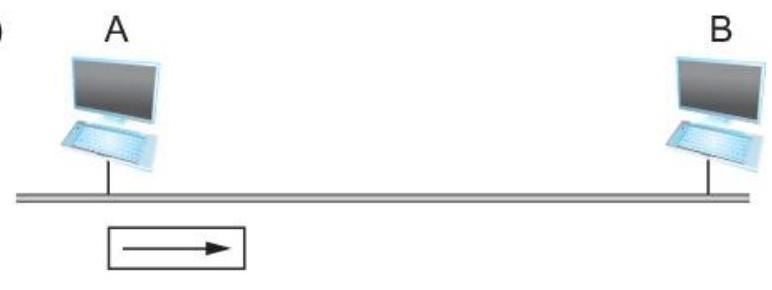
\includegraphics[max width=\textwidth]{2023_01_13_b07e3b4bcffdaab9792bg-121}
\end{center}

(b)

\begin{center}
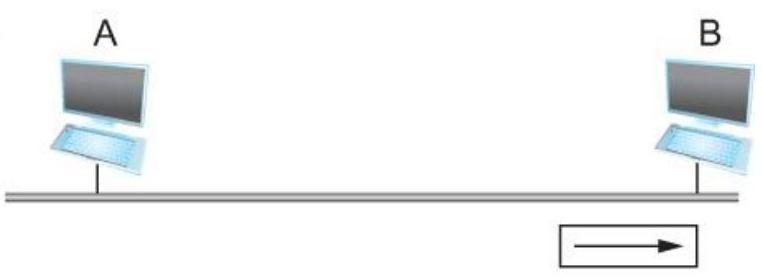
\includegraphics[max width=\textwidth]{2023_01_13_b07e3b4bcffdaab9792bg-121(1)}
\end{center}

(c)

\begin{center}
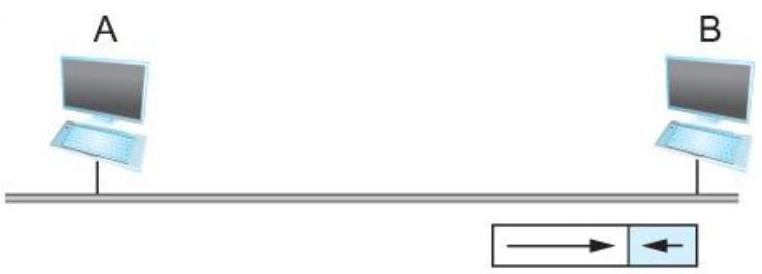
\includegraphics[max width=\textwidth]{2023_01_13_b07e3b4bcffdaab9792bg-121(2)}
\end{center}

(d) $\mathrm{A}$

\begin{center}
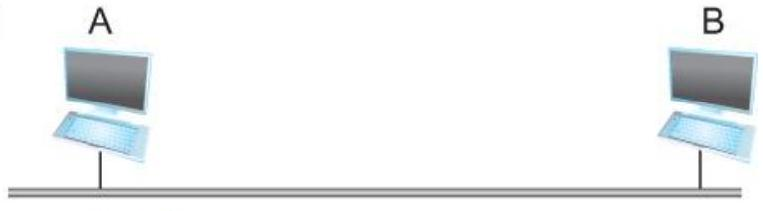
\includegraphics[max width=\textwidth]{2023_01_13_b07e3b4bcffdaab9792bg-121(3)}
\end{center}

Worst-case scenario:

(a) A sends a frame at time $t$;

(b) A's frame arrives at $\mathrm{B}$ at time $t+d$;

(c) B begins transmitting at time $t+d$ and collides with A's frame;

(d) B's runt (32-bit) frame arrives at $\mathrm{A}$ at time $t+2 d$.

\section{Ethernet Transmitter Algorithm}
\section{- Consider that a maximally configured Ethernet is 2500 $\mathrm{m}$ long, and there may be up to four repeaters between any two hosts, the round trip delay has been determined to be $51.2 \mu \mathrm{s}$ 
 o Which on $10 \mathrm{Mbps}$ Ethernet corresponds to 512 bits}
\section{- The other way to look at this situation,}
o We need to limit the Ethernet's maximum latency to a fairly small value $(51.2 \mu \mathrm{s})$ for the access algorithm to work

\begin{itemize}
  \item Hence the maximum length for the Ethernet is on the order of $\mathbf{2 5 0 0}$ $\mathrm{m}$.
\end{itemize}

\section{Ethernet Transmitter Algorithm}
\begin{itemize}
  \item Once an adaptor has detected a collision, and stopped its transmission, it waits a certain amount of time and tries again.

  \item Each time the adaptor tries to transmit but fails, it doubles the amount of time it waits before trying again.

  \item This strategy of doubling the delay interval between each retransmission attempt is known as Exponential Backoff.

\end{itemize}

\section{Ethernet Transmitter Algorithm}
\begin{itemize}
  \item The adaptor first delays either o or $51.2 \mu \mathrm{s}$, selected at random.

  \item If this effort fails, it then waits $0,51.2,102.4,153.6 \mu \mathrm{s}$ (selected randomly) before trying again;

  \item This is $k^{*} 51.2$ for $k=0,1,2,3$

  \item After the third collision, it waits $k^{*} 51.2$ for $k=0 \ldots 2^{3}-1$ (again selected at random).

  \item In general, the algorithm randomly selects a $k$ between $o$ and $2^{\mathrm{n}}-1$ and waits for $k^{*} 51.2 \mu \mathrm{s}$, where $n$ is the number of collisions experienced so far.

\end{itemize}

\section{Experience with Ethernet}
\begin{itemize}
  \item Ethernets work best under lightly loaded conditions.

  \item Under heavy loads, too much of the network's capacity is wasted by collisions.

  \item Most Ethernets are used in a conservative way.

  \item Have fewer than 200 hosts connected to them which is far fewer than the maximum of 1024.

  \item Most Ethernets are far shorter than $2500 m$ with a round-trip delay of closer to $5 \mu$ s than $51.2 \mu \mathrm{s}$.

  \item Ethernets are easy to administer and maintain.

  \item There are no switches that can fail and no routing and configuration tables that have to be kept up-to-date.

  \item It is easy to add a new host to the network.

  \item It is inexpensive.

\end{itemize}

C Cable is cheap, and only other cost is the network adaptor on each host.

\section{Orientation}
1

2

\begin{itemize}
  \item IP (Internet Protocol) is a Network Layer Protocol.
\end{itemize}

\begin{center}
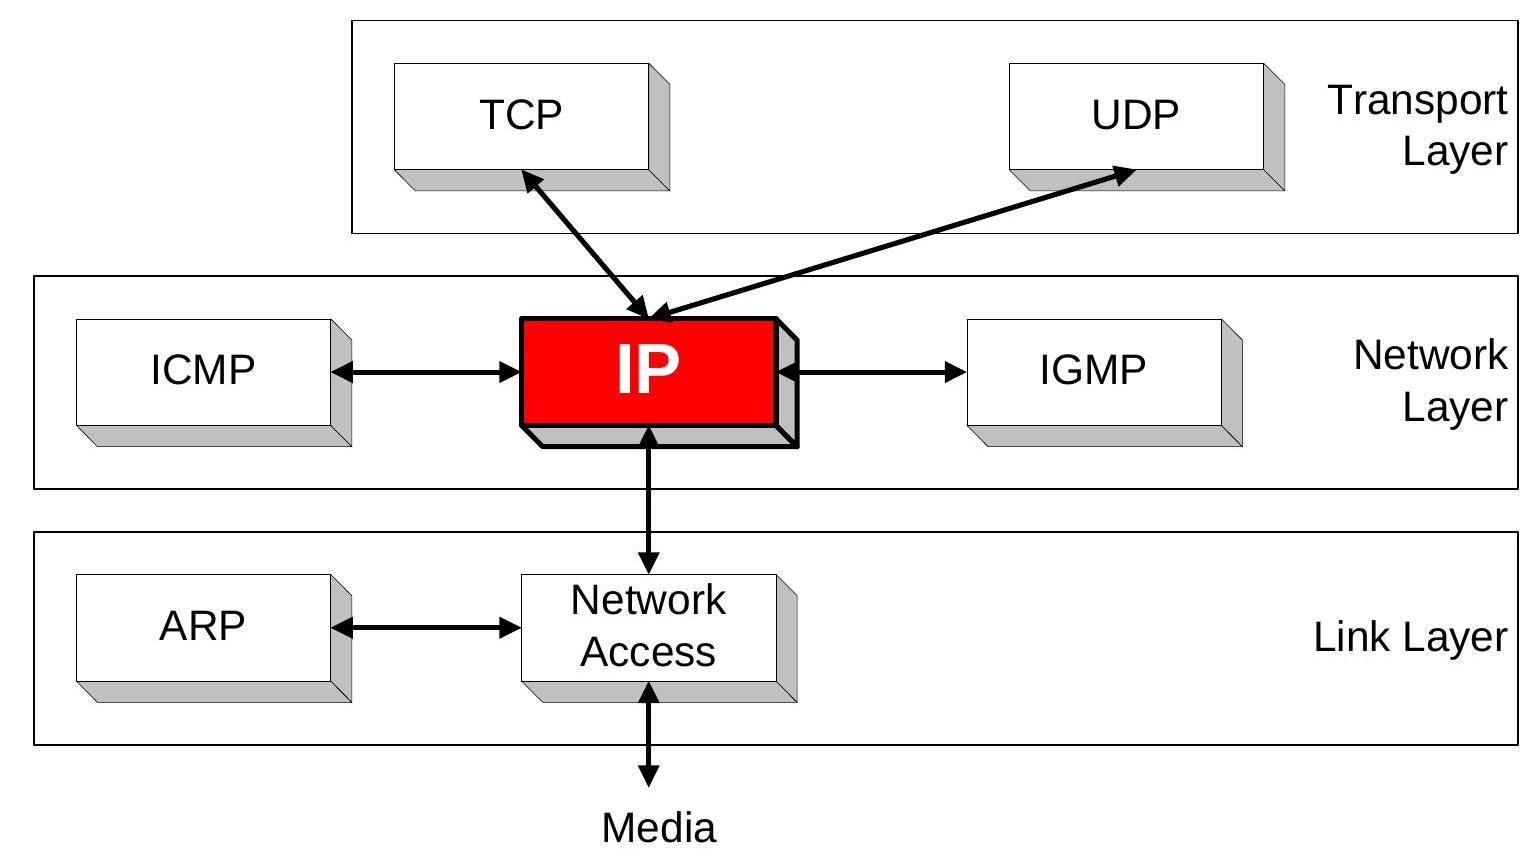
\includegraphics[max width=\textwidth]{2023_01_13_b07e3b4bcffdaab9792bg-127}
\end{center}

\begin{itemize}
  \item IP's current version is Version 4 (IPv4). It is specified in RFC 891.
\end{itemize}

\section{IP: The waist of the hourglass}
1

2

\begin{itemize}
  \item IP is the waist of the liourglass of the Internet protocol architecture

  \item Multiple higher-layer protocols

  \item Multiple lower-layer protocols

  \item Only one protocol at the network

\end{itemize}

\begin{center}
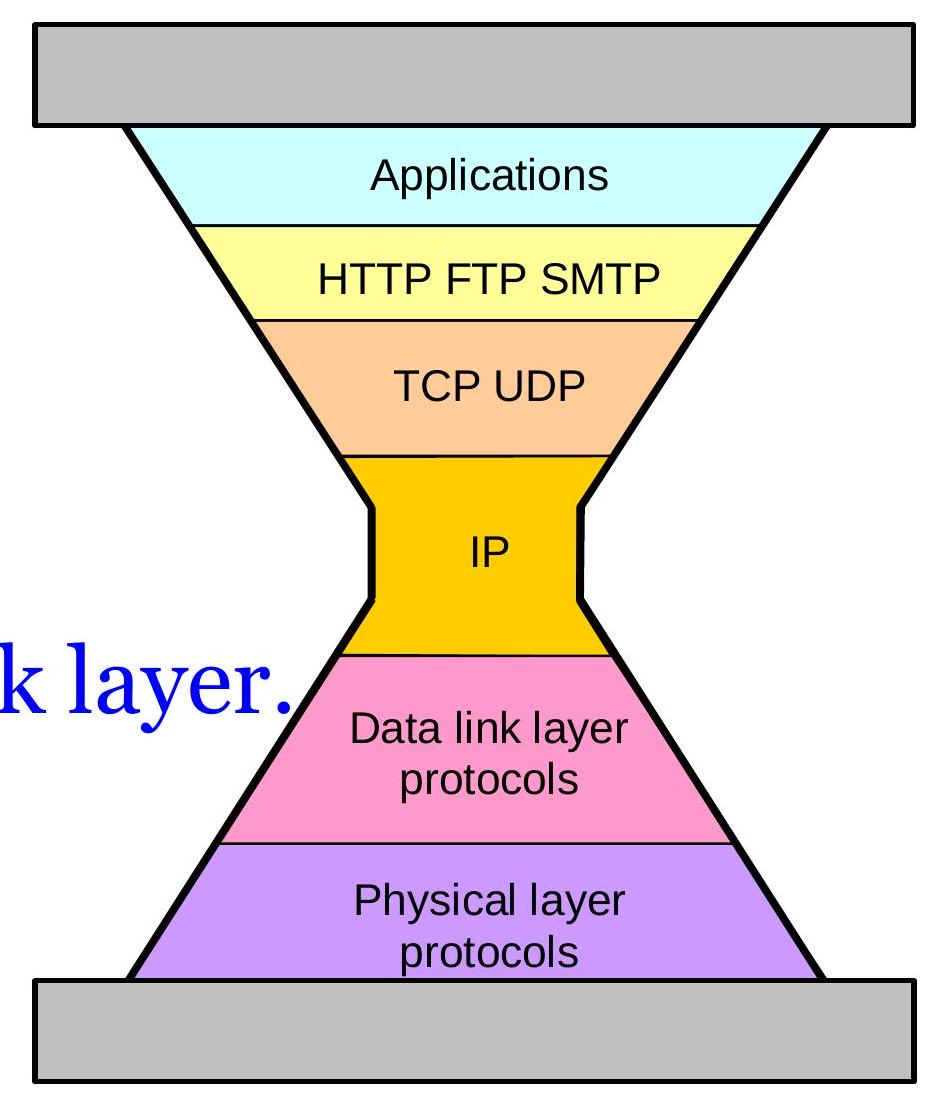
\includegraphics[max width=\textwidth]{2023_01_13_b07e3b4bcffdaab9792bg-128}
\end{center}

\section{Application protocol}
1

2

\begin{itemize}
  \item IP is the highest layer protocol which is implemented at both routers and hosts
\end{itemize}

\begin{center}
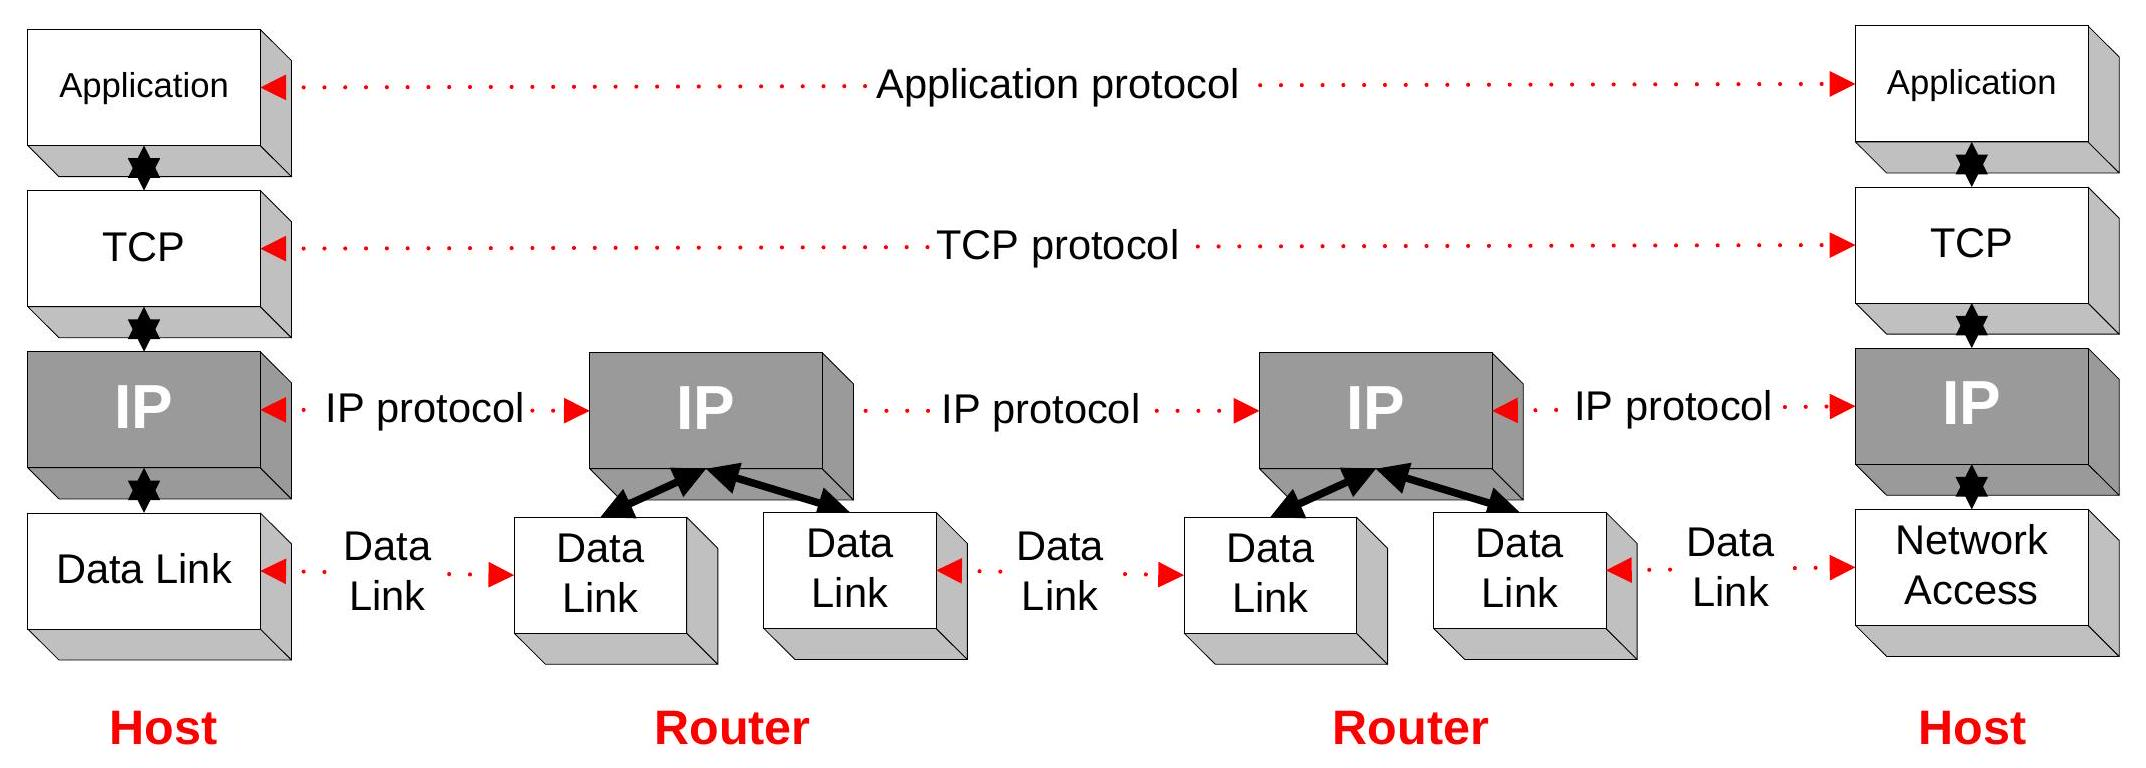
\includegraphics[max width=\textwidth]{2023_01_13_b07e3b4bcffdaab9792bg-129}
\end{center}

\section{IP Service}
\begin{itemize}
  \item Delivery service of IP is minimal 1
3
0

  \item IP provide provides an unreliable connectionless best effort service (also called: "datagram service").

\end{itemize}

o Unreliable: IP does not make an attempt to recover lost packets

o Connectionless: Each packet ("datagram") is handled independently. IP is not aware that packets between hosts may be sent in a logical sequence

o Best effort: IP does not make guarantees on the service (no throughput guarantee, no delay guarantee,..)

\section{- Consequences:}
\begin{itemize}
  \item Higher layer protocols have to deal with losses or with duplicate packets

  \item Packets may be delivered out-of-sequence

\end{itemize}

\section{IP Service}
1

3

\begin{itemize}
  \item IP supports the following services:
\end{itemize}

ane-to-one

cone-to-all

rone-to-several

\begin{center}
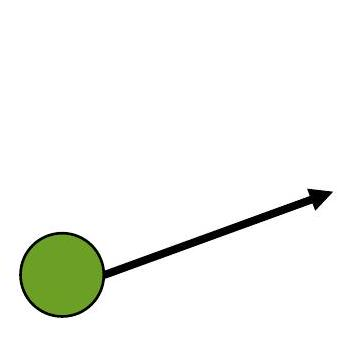
\includegraphics[max width=\textwidth]{2023_01_13_b07e3b4bcffdaab9792bg-131}
\end{center}

unicast

\begin{center}
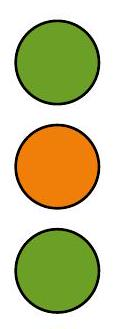
\includegraphics[max width=\textwidth]{2023_01_13_b07e3b4bcffdaab9792bg-131(1)}
\end{center}

broadcast (unicast)

(broadcast)

(multicast)

\begin{center}
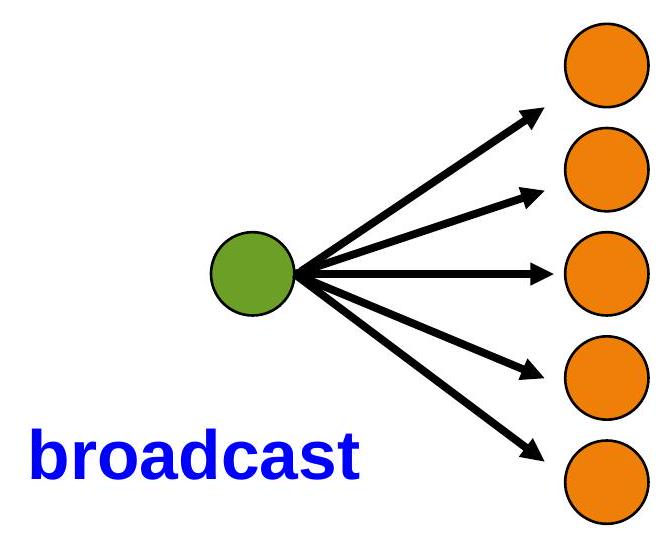
\includegraphics[max width=\textwidth]{2023_01_13_b07e3b4bcffdaab9792bg-131(2)}
\end{center}

\begin{center}
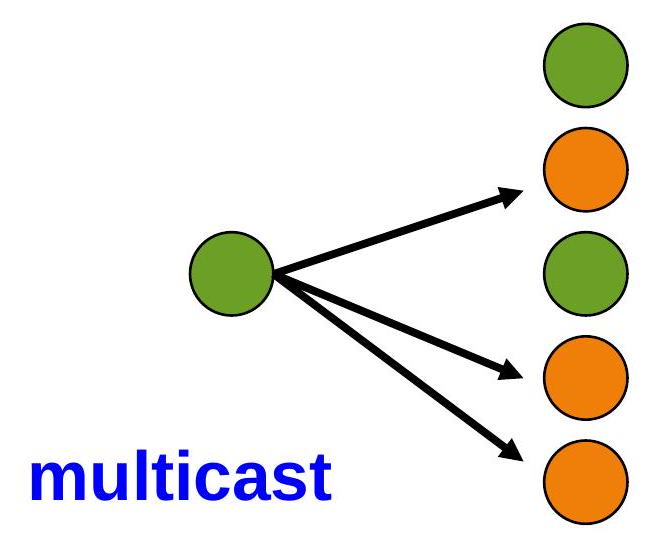
\includegraphics[max width=\textwidth]{2023_01_13_b07e3b4bcffdaab9792bg-131(3)}
\end{center}

\begin{itemize}
  \item IP multicast also supports a many-to-many service.

  \item IP multicast requires support of other protocols (IGMP, multicast routing)

\end{itemize}

\section*{IP Datagram Format }


\begin{itemize}
  \item 20 bytes $\leq$ Header Size $<2^{4}$ x 4 bytes $=60$ bytes

  \item 20 bytes $\leq$ Total Length $<2^{16}$ bytes $=65536$ bytes

\end{itemize}

\begin{center}
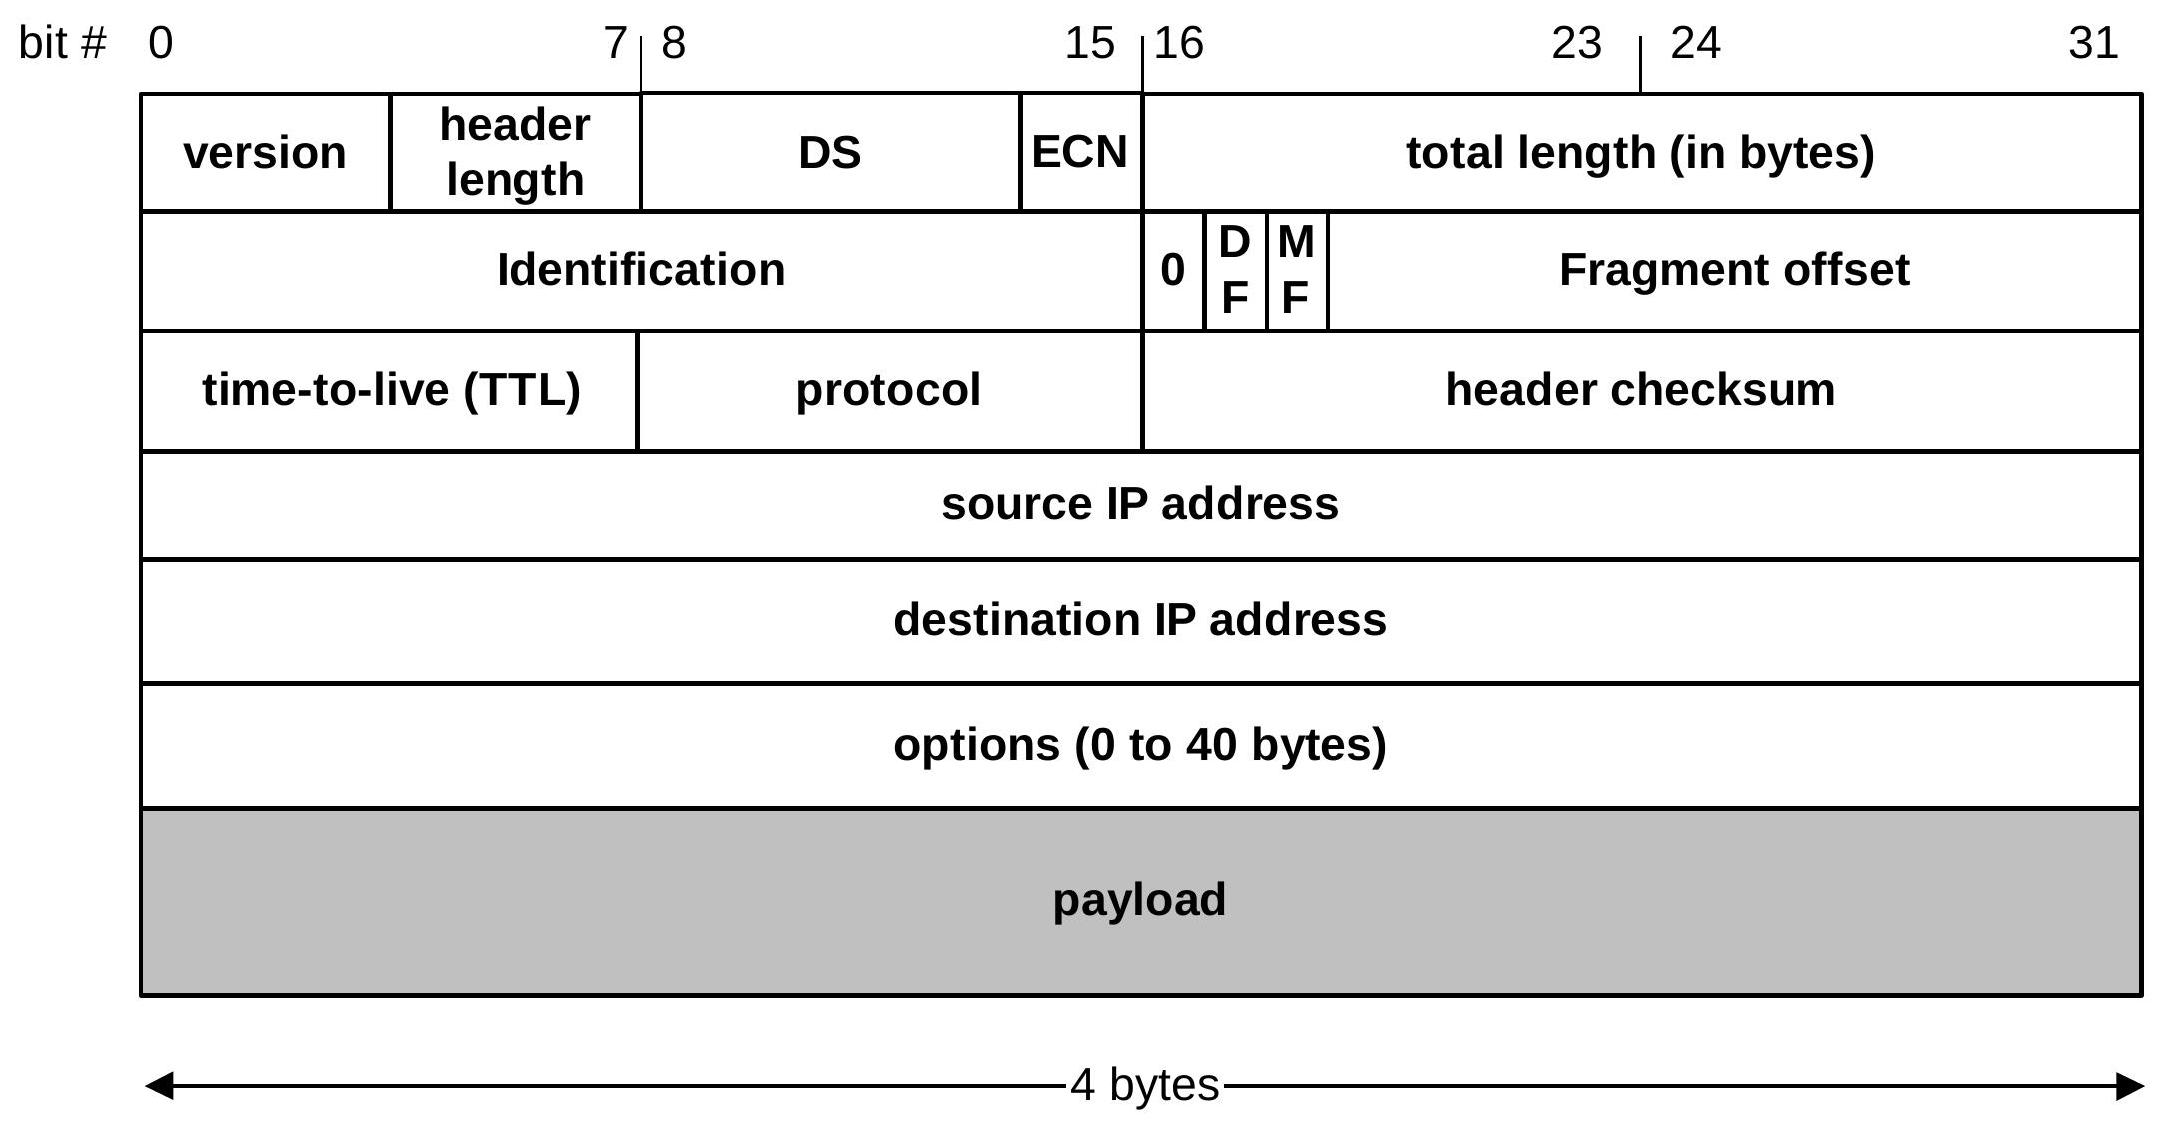
\includegraphics[max width=\textwidth]{2023_01_13_b07e3b4bcffdaab9792bg-132}
\end{center}

\section{IP Datagram Format}
$$
1
$$

3

\begin{itemize}
  \item Question: In which order are the bytes of an IP datagram transmitted?

  \item Answer:

  \item Transmission is row by row

  \item For each row:

\end{itemize}

\begin{enumerate}
  \item First transmit bits $0-7$

  \item Then transmit bits $8-15$

  \item Then transmit bits 16-23

  \item Then transmit bits 24-31

\end{enumerate}

\section{- This is called network byte order or big endian byte ordering.}
\begin{itemize}
  \item Note: Many computers (incl. Intel processors) store 32-bit words in little endian format. Others (incl. Motorola processors) use big endian.
\end{itemize}

\section{Big endian vs. small endian}
\section{1 
 3 
 4}
\begin{itemize}
  \item Conventions to store a multibyte work

  \item Example: a 4 byte Long Integer Byte3 Byte2 Byte1 Byte0

\end{itemize}

\section{Little Endian}
\begin{itemize}
  \item Stores the low-order byte at the lowest address and the highest order byte in the highest address.
\end{itemize}

Base Addresst0 Byte0 Base Addresst1 Byte1 Base Address+2 Byte2 Base Address+3 Byte3

\begin{itemize}
  \item Intel processors use this order
\end{itemize}

\section{Big Endian}
\begin{itemize}
  \item Stores the high-order byte at the lowest address, and the low-order byte at the highest address.
Base Address+0 Byte3
Base Addresst1 Byte2
Base Addresst2 Byte1
Base Address+3 Byte0
\end{itemize}

Motorola processors use big endian.

\section*{Fields of the IP Header }


\begin{itemize}
  \item Version (4 bits): current version is 4, next version will be 6.

  \item Header length (4 bits): length of IP header, in multiples of 4 bytes

  \item DS/ECN field (1 byte)

\end{itemize}

o This field was previously called as Type-of-Service (TOS) field. The role of this field has been re-defined, but is "backwards compatible" to TOS interpretation

o Differentiated Service (DS) (6 bits):

\begin{itemize}
  \item Used to specify service level (currently not supported in the Internet)
\end{itemize}

o Explicit Congestion Notification (ECN) (2 bits):

\begin{CJK}{UTF8}{mj}乂\end{CJK} New feedback mechanism used by TCP

\section*{Fields of the IP Header }


\begin{itemize}
  \item Identification (16 bits): Unique identification of a datagram from a host. Incremented whenever a datagram is transmitted

  \item Flags (3 bits):

  \item First bit always set to 0

\end{itemize}

o DF bit (Do not fragment)

o MF bit (More fragments)

Will be explained later $\rightarrow$ Fragmentation

\section{Fields of the IP Header}
1

3

\begin{itemize}
  \item Time To Live (TTL) (17byte):
\end{itemize}

o Specifies longest paths before datagram is dropped

o Role of TTL field: Ensure that packet is eventually dropped when a routing loop occurs

Used as follows:

o Sender sets the value (e.g., 64)

o Each router decrements the value by 1

o When the value reaches 0 , the datagram is dropped

\section{Fields of the IP Header}
1

\begin{itemize}
  \item Protocol (1 byte):
\end{itemize}

3

8

\begin{itemize}
  \item Specifies the higher-layer protocol.
\end{itemize}

\begin{itemize}
  \item Used for demultiplexing to higher layers.
\end{itemize}

\begin{center}
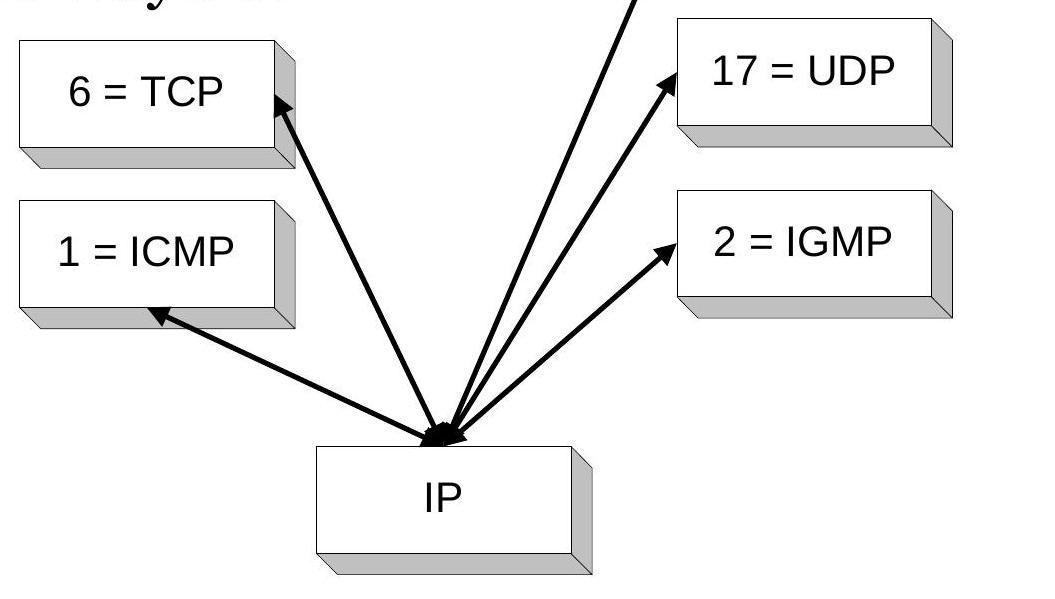
\includegraphics[max width=\textwidth]{2023_01_13_b07e3b4bcffdaab9792bg-138}
\end{center}

\begin{itemize}
  \item Header checksum (2 bytes): A simple 16-bit long checksum which is computed for the header of the datagram.
\end{itemize}

\section*{Fields of the IP Header }


\section{- Options:}
9

\begin{itemize}
  \item Security restrictions
\end{itemize}

Record Route: each router that processes the packet adds its IP address to the header.

Timestamp: each router that processes the packet adds its IP address and time to the header.

(loose) Source Routing: specifies a list of routers that must be traversed.

\begin{itemize}
  \item (strict) Source Routing: specifies a list of the only routers that can be traversed.
\end{itemize}

\section{- Padding: Padding bytes are added to ensure that header ends on a 4-byte boundary}
\section{Maximum Transmission Unit}
1

4

\begin{itemize}
  \item Maximum size of IP datagram is 65535 , but the data link layer protocol generally imposes a limit that is much smaller

  \item Example:

\end{itemize}

o Ethernet frames have a maximum payload of 1500 bytes

$\rightarrow$ IP datagrams encapsulated in Ethernet frame cannot be longer than 1500 bytes

\begin{itemize}
  \item The limit on the maximum IP datagram size, imposed by the data link protocol is called maximum transmission unit (MTU)

  \item MTUs for various data link protocols:

\end{itemize}

Ethernet: $\quad 1500$

802.3:

802.5: 1492

4464 FDDI: $\quad 4352$

ATM AAL5: 9180

PPP:

\section*{IP Fragmentation }


\begin{itemize}
  \item What if the size of an IP datagram exceeds the MTU? IP datagram is fragmented into smaller units.

  \item What if the route contains networks with different MTUs?

\end{itemize}

\begin{center}
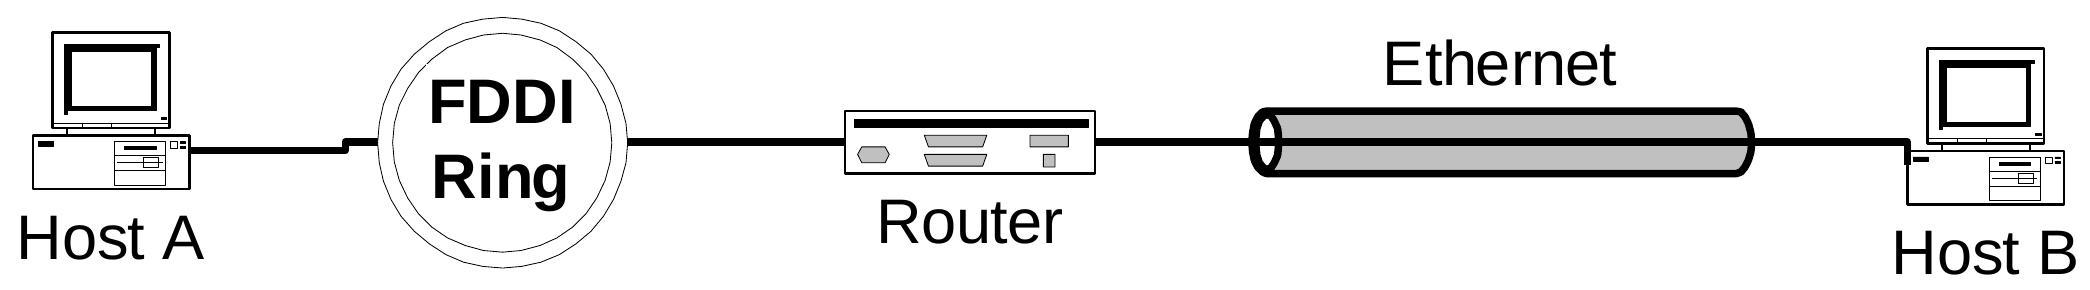
\includegraphics[max width=\textwidth]{2023_01_13_b07e3b4bcffdaab9792bg-141}
\end{center}

MTUs: FDDI: 4352

Ethernet: 1500

\begin{itemize}
  \item Fragmentation:

  \item IP router splits the datagram into several datagram

  \item Fragments are reassembled at receiver

\end{itemize}

\section*{Where is Fragmentation done? }


\begin{itemize}
  \item Fragmentation can be done at the sender or at intermediate routers
\end{itemize}

×he same datagram can be fragmented several times.

 Reassembly of original datagram is only done at destination hosts !!
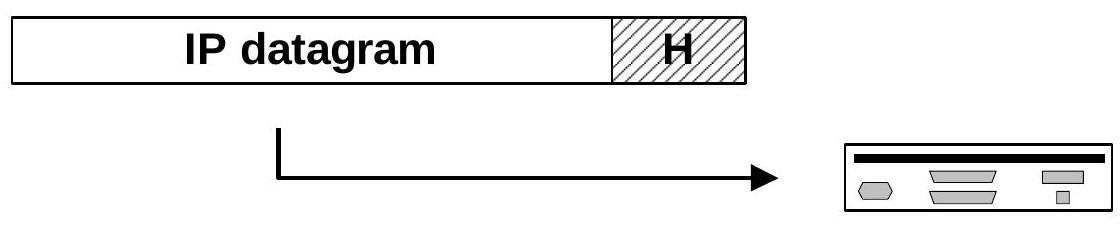
\includegraphics[max width=\textwidth, center]{2023_01_13_b07e3b4bcffdaab9792bg-142}

Fragment 2

42

Fragment 1

(1)

Router

\section{What's involved in Fragmentation?}
\begin{itemize}
  \item The following fields in the IP header are involved:
\end{itemize}

\begin{center}
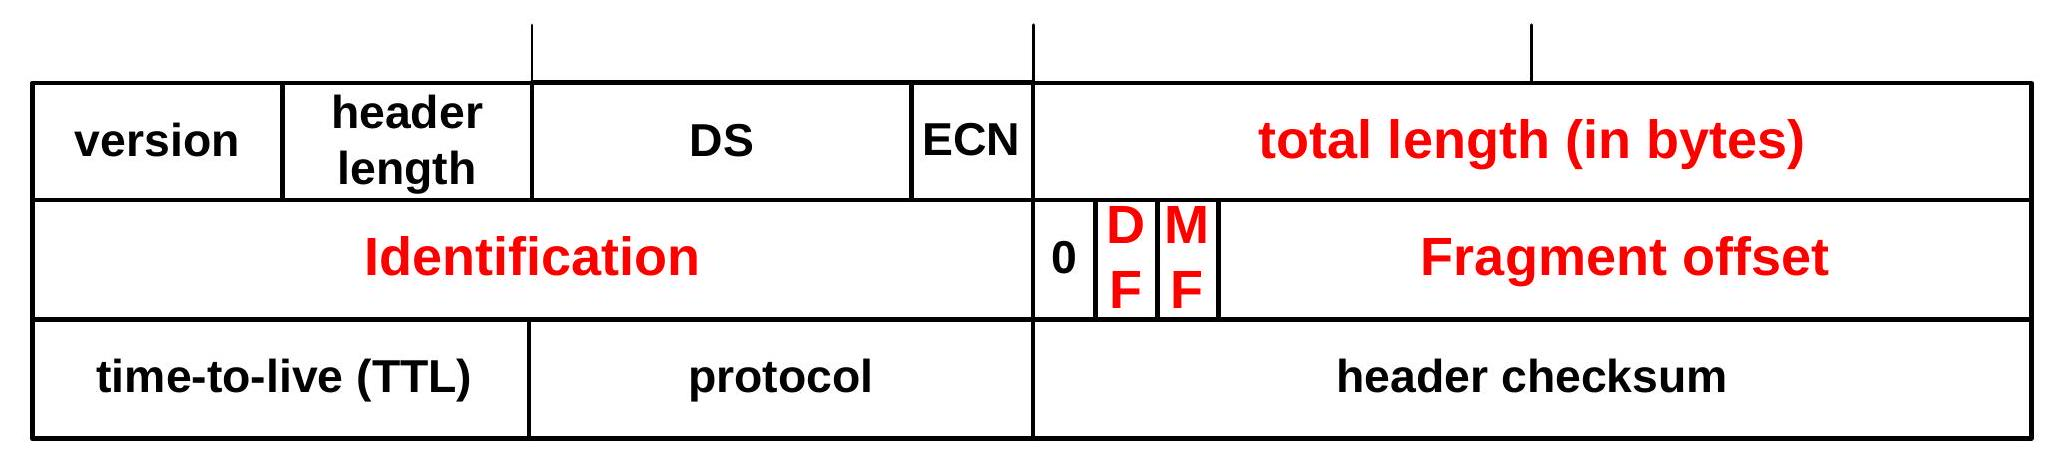
\includegraphics[max width=\textwidth]{2023_01_13_b07e3b4bcffdaab9792bg-143}
\end{center}

Identification

Flags When a datagram is fragmented, the identification is the same in all fragments

DF bit is set: Datagram cannot be fragmented and must be discarded if MTU is too small

MF bit set: This datagram is part of a fragment and an additional fragment follows this one

\section{What's involved in Fragmentation?}
\begin{itemize}
  \item The following fields in the IP header are involved:
\end{itemize}

\begin{center}
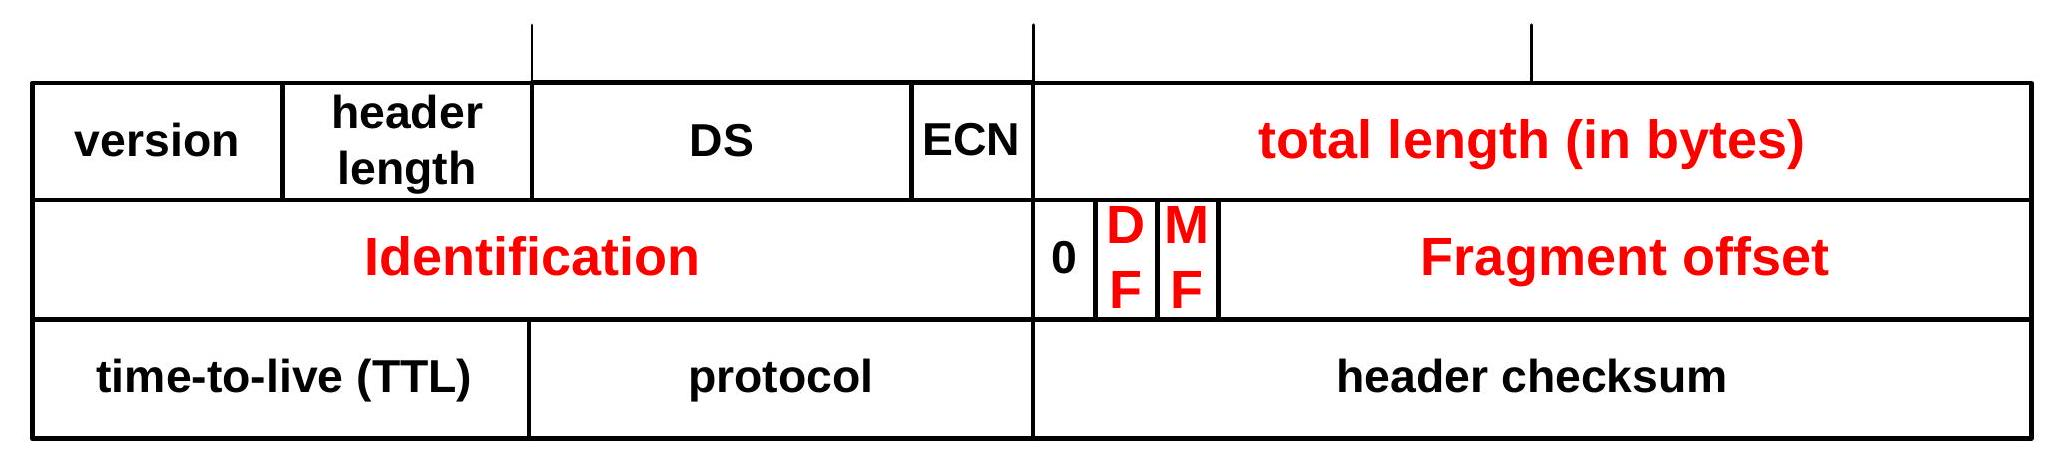
\includegraphics[max width=\textwidth]{2023_01_13_b07e3b4bcffdaab9792bg-144}
\end{center}

Fragment offset Offset of the payload of the current fragment in the original datagram Total length

Total length of the current fragment

\section*{Example of Fragmentation }


\begin{itemize}
  \item A datagram with size 2400 bytes isust be fragmented according to an MTU limit of 1000 bytes
\end{itemize}

Header length: 20 Total length: 2400 Identification: 0xa428

DF flag: 0 MF flag: 0

Fragment offset: 0 Header length: 20

Total length: 448 Identification: 0xa428

DF flag: 0

MF flag: 0

Fragment offset: 244 Header length: 20

Total length: 996 Identification: 0xa428 DF flag: 0 MF flag: 1 Fragment offset: 122 Header length: 20 Total length: 996 Identification: 0xa428 DF flag: 0 MF flag: 1 fragment offset: 0
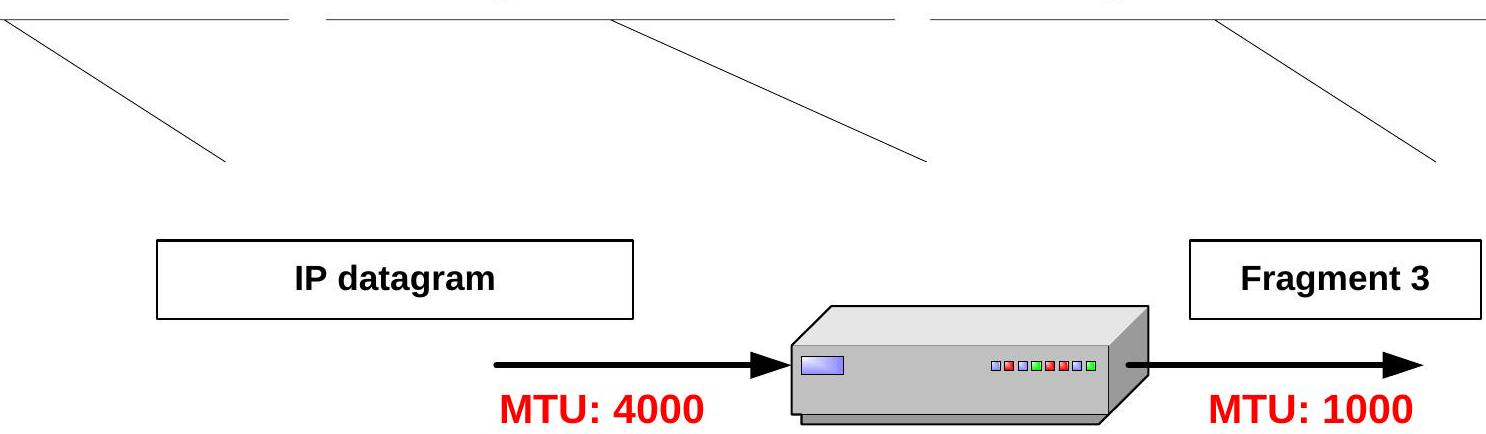
\includegraphics[max width=\textwidth, center]{2023_01_13_b07e3b4bcffdaab9792bg-145}

Fragment 2

Fragment 1

Router

\section{Determining the length of fragments}
1

4

\begin{itemize}
  \item To determine the size of the fragments we recall that, since there are only 13 bits available for the fragment offset, the offset is given as a multiple of eight bytes.

  \item a result, the first and second fragment have a size of 996 bytes (and not 1000 bytes). This number is chosen since 976 is the largest number smaller than $1000-20=980$ that is divisible by eight.

  \item The payload for the first and second fragments is 976 bytes long, with bytes o through 975 of the original IP payload in the first fragment, and bytes 976 through 1951 in the second fragment.

  \item The payload of the third fragment has the remaining 428 bytes, from byte 1952 through 2379.

  \item With these considerations, we can determine the values of the fragment offset, which are $0,976 / 8=122$, and $1952 / 8=$ 244 , respectively, for the first, second and third fragment.

\end{itemize}

\section{IP Addressing}
\section*{What is an IP address? }
\section{- An unique identifier for a computer or device (host) on a TCP/IP network}
\section{- A 32-bit binary number usually represented as 4 decimal numbers separated by a period}


\section*{What is an IP address? }
\section{- Each address is $3^{2}$ bits wide}
\begin{itemize}
  \item Valid addresses can range from 0.0.0.0 to 255.255.255.255
\end{itemize}



\section*{What is an IP address? }
\section{Theoretically, a total of $\approx 4.3$ billion addresses are available}


\section{Two addresses in one...}
\section{Each address consists of two parts}
\section{The network address}
\section{The host address}
\section{Other systems may use more than one address (Ex: IPX)}
\section{The Five Network Classes}
\begin{enumerate}
  \item Class $\mathrm{A}-$ begins with 0
\end{enumerate}

\begin{itemize}
  \item $00000001\left(1_{10}\right)$ to $01111111\left(126_{10}\right)^{*}$
\end{itemize}

\begin{enumerate}
  \setcounter{enumi}{1}
  \item Class $\mathbf{B}-$ begins with $\mathbf{1 0}$
\end{enumerate}

\begin{itemize}
  \item $10000000\left(128_{10}\right)$ to $10111111\left(191_{10}\right)$
\end{itemize}

\section{Class $\mathrm{C}-$ begins with $\mathbf{1 1 0}$}
\begin{itemize}
  \item $11000000\left(192_{10}\right)$ to $11011111\left(223_{10}\right)$
\end{itemize}

$* 01111111=127_{10}$

\section{Addresses beginning with 127 are reserved for loopback (127.0.0.1 is YoU)}
\section{The Five Network Classes}
\section{Class $\mathrm{D}$ - begins with 1110}
\begin{itemize}
  \item $224_{10}$ to $239_{10}$

  \item Reserved for multicasting

\end{itemize}

\section{Class E - begins with $\mathbf{1 1 1 1}$}
\begin{itemize}
  \item $240_{10}$ to $254_{10}$

  \item Reserved for future use

\end{itemize}

\section{These should not be used for host addressing}
\section*{Which part belongs to the network and which part belongs to the node? }

\section{Class B - XXXXXXXX.XXXXXXXX.yyyyyyyy.yyyyyyyy}
\section{Class C - XXXXXXXX.XXXXXXXX.XXXXXXXX.yyyyyyyy}
\section{Where $X=$ Network and $y=$ node}
\section{IP Addresses*}
\section{Class $1^{\text {st }}$ Octet Networks Ids Host IDs}
\begin{center}
\begin{tabular}{|c|c|c|c|}
\hline
$A$ & $1-126$ & $2^{7}=126$ & $2^{24}=16 M$ \\
\hline
$B$ & $128-191$ & $2^{14}=16 K$ & $2^{16}=64 K$ \\
\hline
$C$ & $192-223$ & $2^{21}=2 M$ & $2^{8}=255$ \\
\hline
\end{tabular}
\end{center}

\section{There are three IP network addresses reserved for private networks}
\begin{enumerate}
  \item $10.0 .0 .0 / 8$

  \item $172.16 .0 .0 / 12$

  \item $192.168 .0 .0 / 16$

\end{enumerate}

\section{These can be used by anyone setting up an internal network.}
\section{Routers will never forward packets coming from these addresses.}
\section{Subnetting}
...can be done for a variety of reasons

o Organization

\begin{itemize}
  \item Use of different physical media

  \item Preservation of address space

\end{itemize}

o Security

\begin{itemize}
  \item The most common reason is to control network traffic
\end{itemize}

\section{Subnetting}
\begin{itemize}
  \item In an Ethernet network, all nodes on a segment see all packets transmitted by other nodes on that segment

  \item Performance can be adversely affected under heavy traffic loads

  \item A router is used to connect IP networks to minimize the amount of traffic each segment must receive

\end{itemize}

\section{Subnet masking}
\begin{itemize}
  \item Applying a subnet mask allows you to identify the network and node parts of the address. A router will then determine whether the address is local or remote.

  \item Network bits are masked as 1s

  \item Node bits are masked as os

  \item Class A - 255.0.0.0

\end{itemize}

o 11111111.00000000.00000000.00000000

\begin{itemize}
  \item Class B - 255.255.0.0
\end{itemize}

O 11111111.11111111.00000000.00000000

\begin{itemize}
  \item Class C - 255.255.255.0
\end{itemize}

o 11111111.11111111.11111111.00000000

\section{Subnet masking}
cil c: WINDOWS system32 cmd.exe

$P: \backslash>$ ipconfig $/ \mathbf{a l l}$

Windows IP Conf iguration

Host Name : - $-\cdot \cdot \cdot \cdot \cdot \cdot \cdot \cdot \cdot \cdot=$ D201B-01

\begin{center}
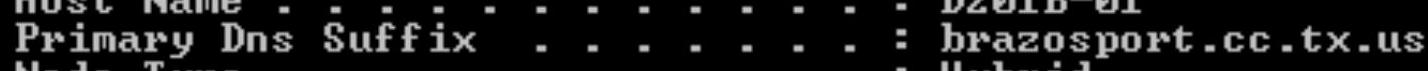
\includegraphics[max width=\textwidth]{2023_01_13_b07e3b4bcffdaab9792bg-160}
\end{center}

Node Type ... . . . . . . . . Hybrid

IP Routing Enabled: : : : : : : No

WINS Proxy Enabled.: :.:-:.: No

DNS Suffix Search List... . . : \href{http://Hrazosport.cc.tx.us}{Hrazosport.cc.tx.us}

\href{http://cc.tx.us}{cc.tx.us}

\href{http://tx.us}{tx.us}

Ethernet adapter Local Area Connection:

Connection-specific DNS Suffix

\begin{center}
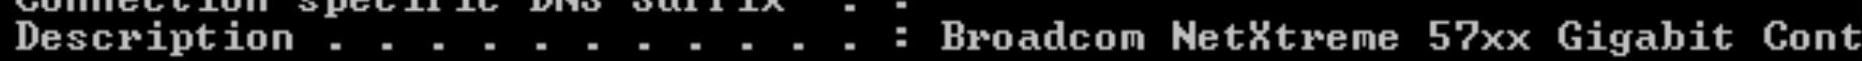
\includegraphics[max width=\textwidth]{2023_01_13_b07e3b4bcffdaab9792bg-160(1)}
\end{center}

rollers

Physical Address . . . . . . . . . : 00-19-B9-46-38-F2

Dhcp Enabled. . . . . . . . . . . : No

\begin{center}
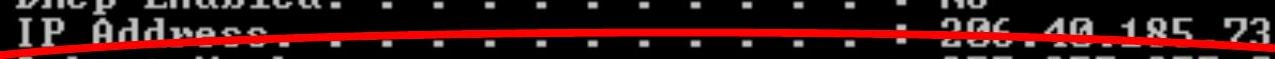
\includegraphics[max width=\textwidth]{2023_01_13_b07e3b4bcffdaab9792bg-160(2)}
\end{center}

\begin{center}
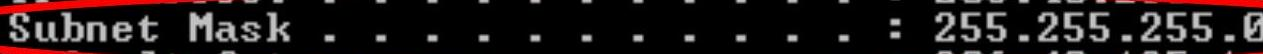
\includegraphics[max width=\textwidth]{2023_01_13_b07e3b4bcffdaab9792bg-160(3)}
\end{center}

\begin{center}

\includegraphics[max width=\textwidth]{2023_01_13_b07e3b4bcffdaab9792bg-160(4)}
\end{center}

DNS Seruers. $=.-.=.-.=-206.40 .177 .10$

$206.40 .177 .11$

$P: \backslash>$

\section{Subnet masking}
\begin{itemize}
  \item Performing a bitwise logical AND between the IP address and the subnet mask results in the network address

  \item Ex: Class - B 140.179.240.200

\end{itemize}

10001100.10110011.11110000.11001000

11111111.11111111.00000000.00000000

10001100.10110011.00000000.00000000

Network Address $=140.179 .000 .000$

\section*{A Few Rules... }
\section{Each device on a node has a unique MAC address}
\section{Each device on a node needs a unique IP address}
\section{All devices on the same physical segment share a common network ID (subnet mask)}


\section{Address Resolution Protocol (ARP)}
\begin{itemize}
  \item Before an IP packet can be forwarded to another host, the MAC address (usually 6 bytes written in hex (Ex: 02-FE-874A-8C-A9) of the receiving machine must be known

  \item ARP determines the MAC addresses that correspond to an IP address

  \item A router will choose direct paths for the network packets based on the addressing of the IP frame it is handling (different routes to different networks)

\end{itemize}

\section{Address Resolution Protocol (ARP)}
\section*{Internet and Data Link Layer Addresses }
\begin{itemize}
  \item Each host and router on a subnet needs a data link layer address to specify its address on the subnet
\end{itemize}

\begin{center}
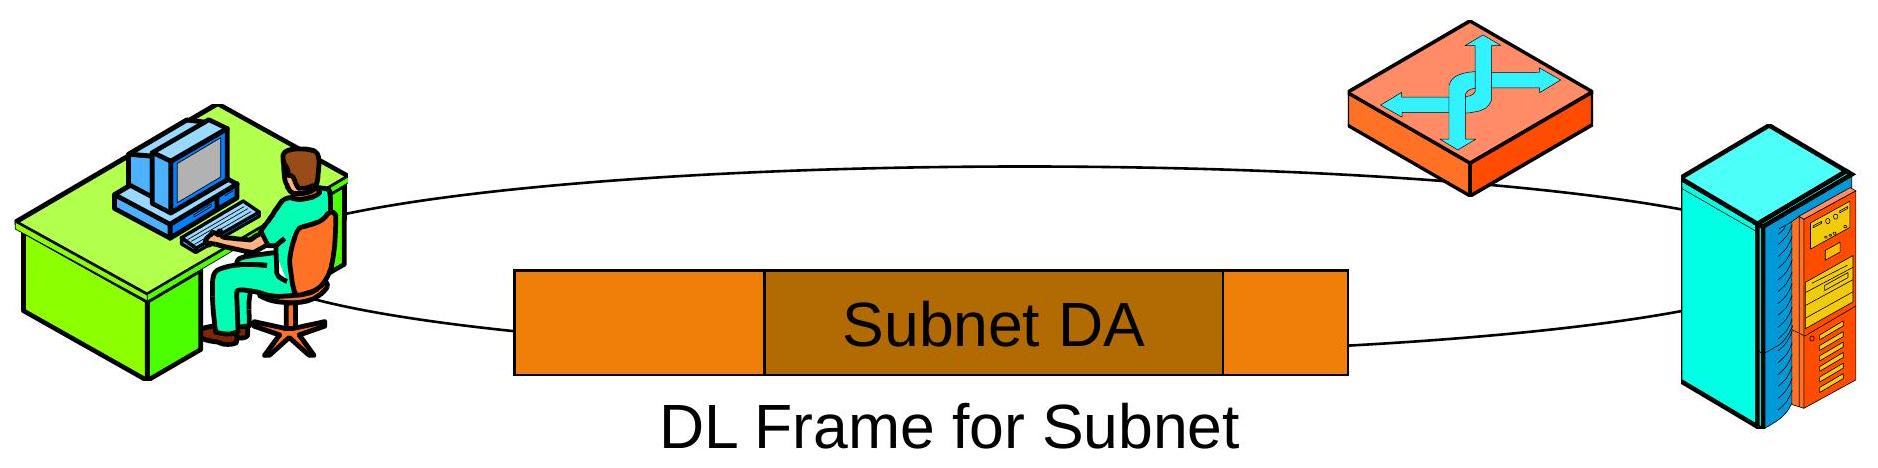
\includegraphics[max width=\textwidth]{2023_01_13_b07e3b4bcffdaab9792bg-165}
\end{center}

\section{Addresses}
\begin{itemize}
  \item Each host and router also needs an IP address at the internet layer to designate its position in the overall Internet
\end{itemize}

\begin{center}
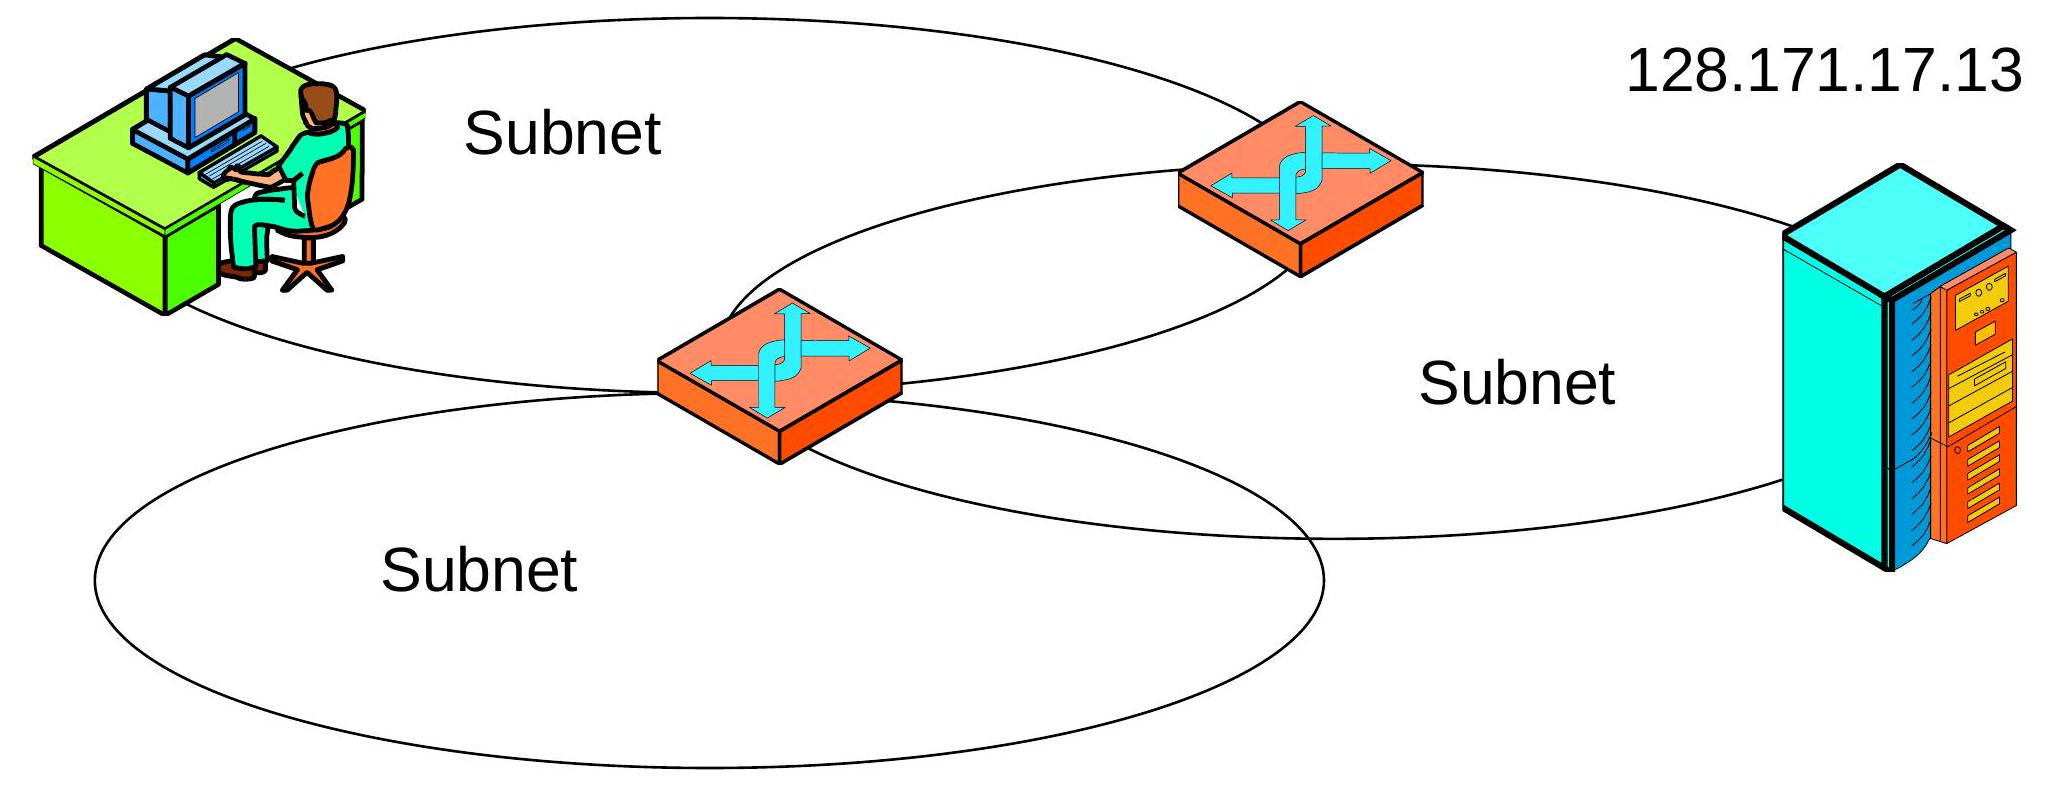
\includegraphics[max width=\textwidth]{2023_01_13_b07e3b4bcffdaab9792bg-166}
\end{center}

\section{Internet and Data Link Addresses Serve Different Purposes}
\begin{center}

\includegraphics[max width=\textwidth]{2023_01_13_b07e3b4bcffdaab9792bg-167}
\end{center}

\begin{itemize}
  \item IP address
\end{itemize}

o To guide delivery to destination host across the Internet (across multiple networks)

\begin{itemize}
  \item Subnet Address
\end{itemize}

o To guide delivery between two hosts, two routers, and a host and router within a single subnet

\begin{itemize}
  \item Same LAN, Frame Relay network, etc.
\end{itemize}

\section{Analogy}
\begin{itemize}
  \item In company, each person has a company-wide ID number (like IP address)

  \item In company, person also has a local office number in a building

  \item Paychecks are made out to ID numbers

  \item For delivery, also need to know office number

\end{itemize}

\section{Address Resolution}
\begin{center}

\includegraphics[max width=\textwidth]{2023_01_13_b07e3b4bcffdaab9792bg-169}
\end{center}

\begin{itemize}
  \item Problem
\end{itemize}

o Router knows that destination host is on its subnet based on the IP address of an arriving packet

o Does not know the destination host's subnet address, so cannot deliver the packet across the subnet

\begin{center}
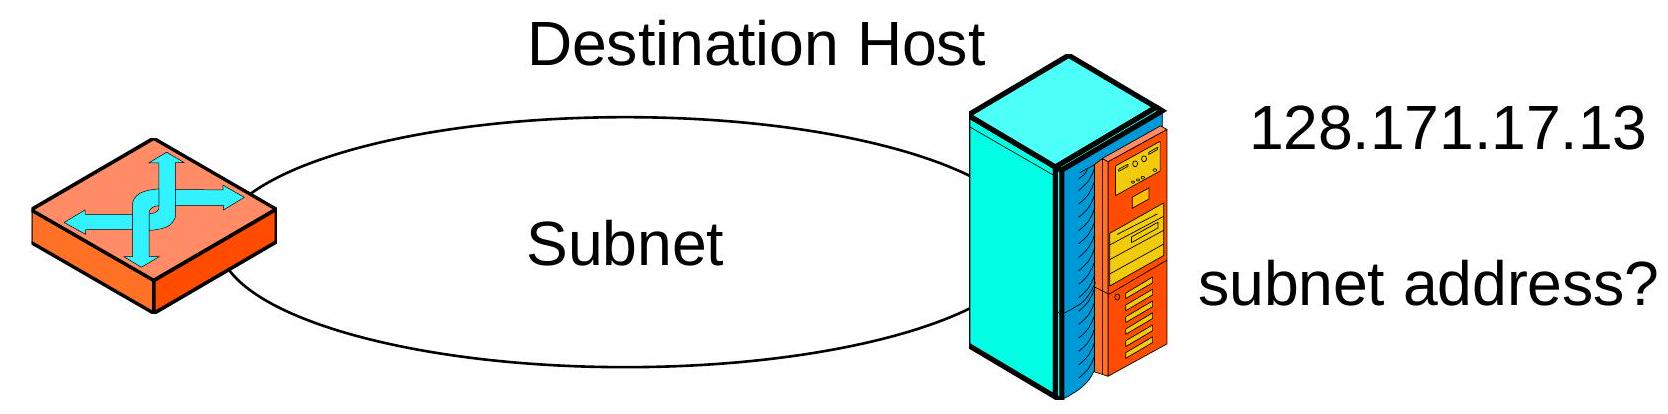
\includegraphics[max width=\textwidth]{2023_01_13_b07e3b4bcffdaab9792bg-169(1)}
\end{center}

\section{Address Resolution Protocol (ARP)}
\begin{itemize}
  \item Router creates an ARP Request message to be
sent to all hosts on the subnet.

  \item Address resolution protocol message asks “Who has IP address 128.171.17.13?"

  \item Passes ARP request to data link layer process for delivery

\end{itemize}

\begin{center}
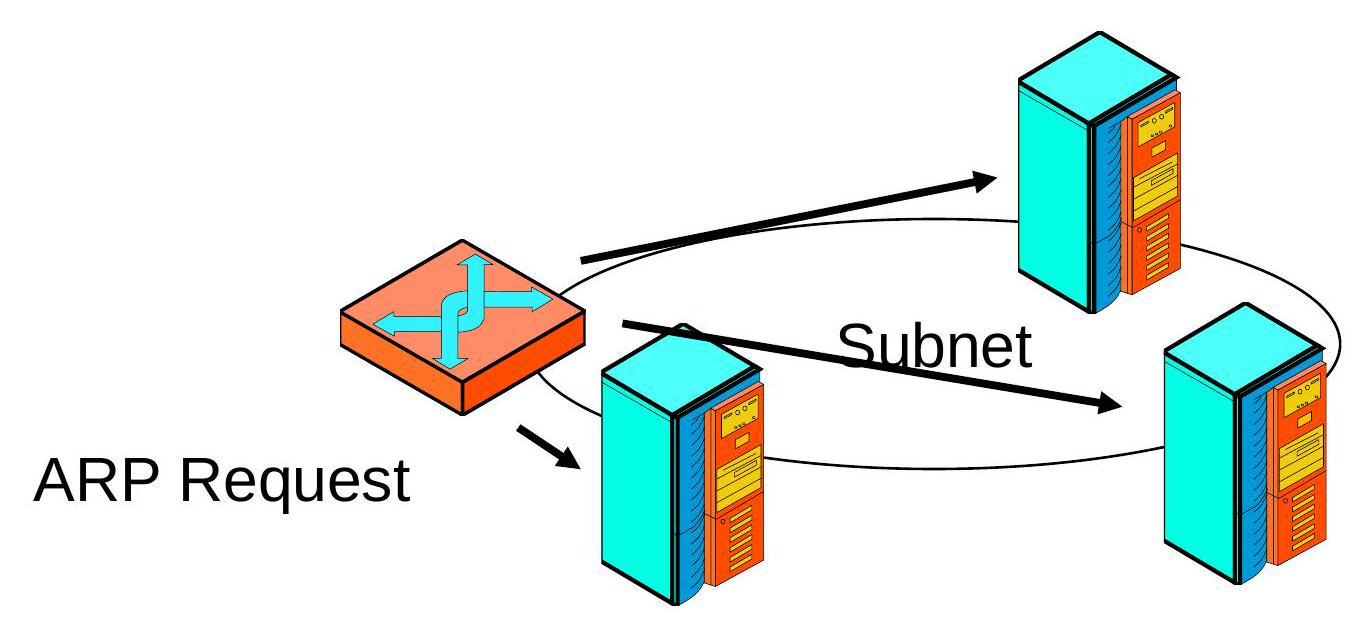
\includegraphics[max width=\textwidth]{2023_01_13_b07e3b4bcffdaab9792bg-170}
\end{center}

\section{Address Resolution Protocol (ARP)}
\section{- Data link process of router broadcasts the ARP Request message to all hosts on the subnet.}
\section{o On a LAN, MAC address of 48 ones tells all stations to pay attention to the frame}
\begin{center}
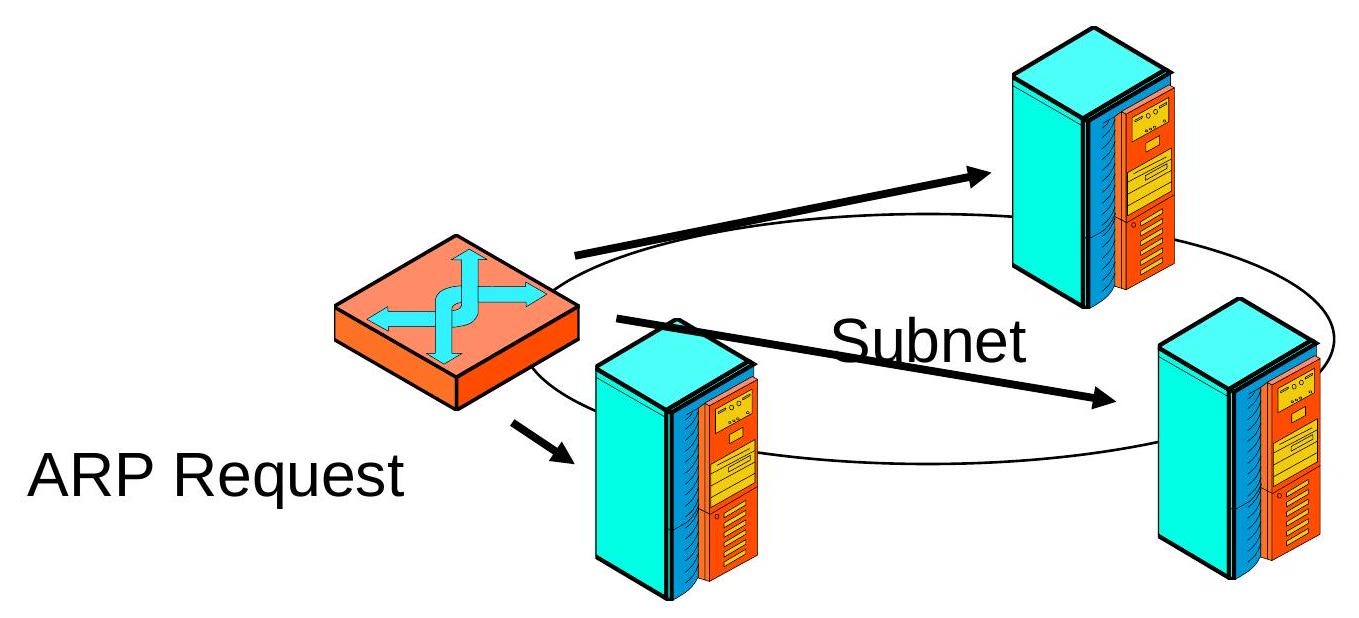
\includegraphics[max width=\textwidth]{2023_01_13_b07e3b4bcffdaab9792bg-171}
\end{center}

\section{Address Resolution Protocol )}
\begin{itemize}
  \item Host with IP address 128.171.17.13 responds

  \item Internet process creates an ARP response message

  \item Contains the destination host's subnet address (48-bit MAC address on a LAN)
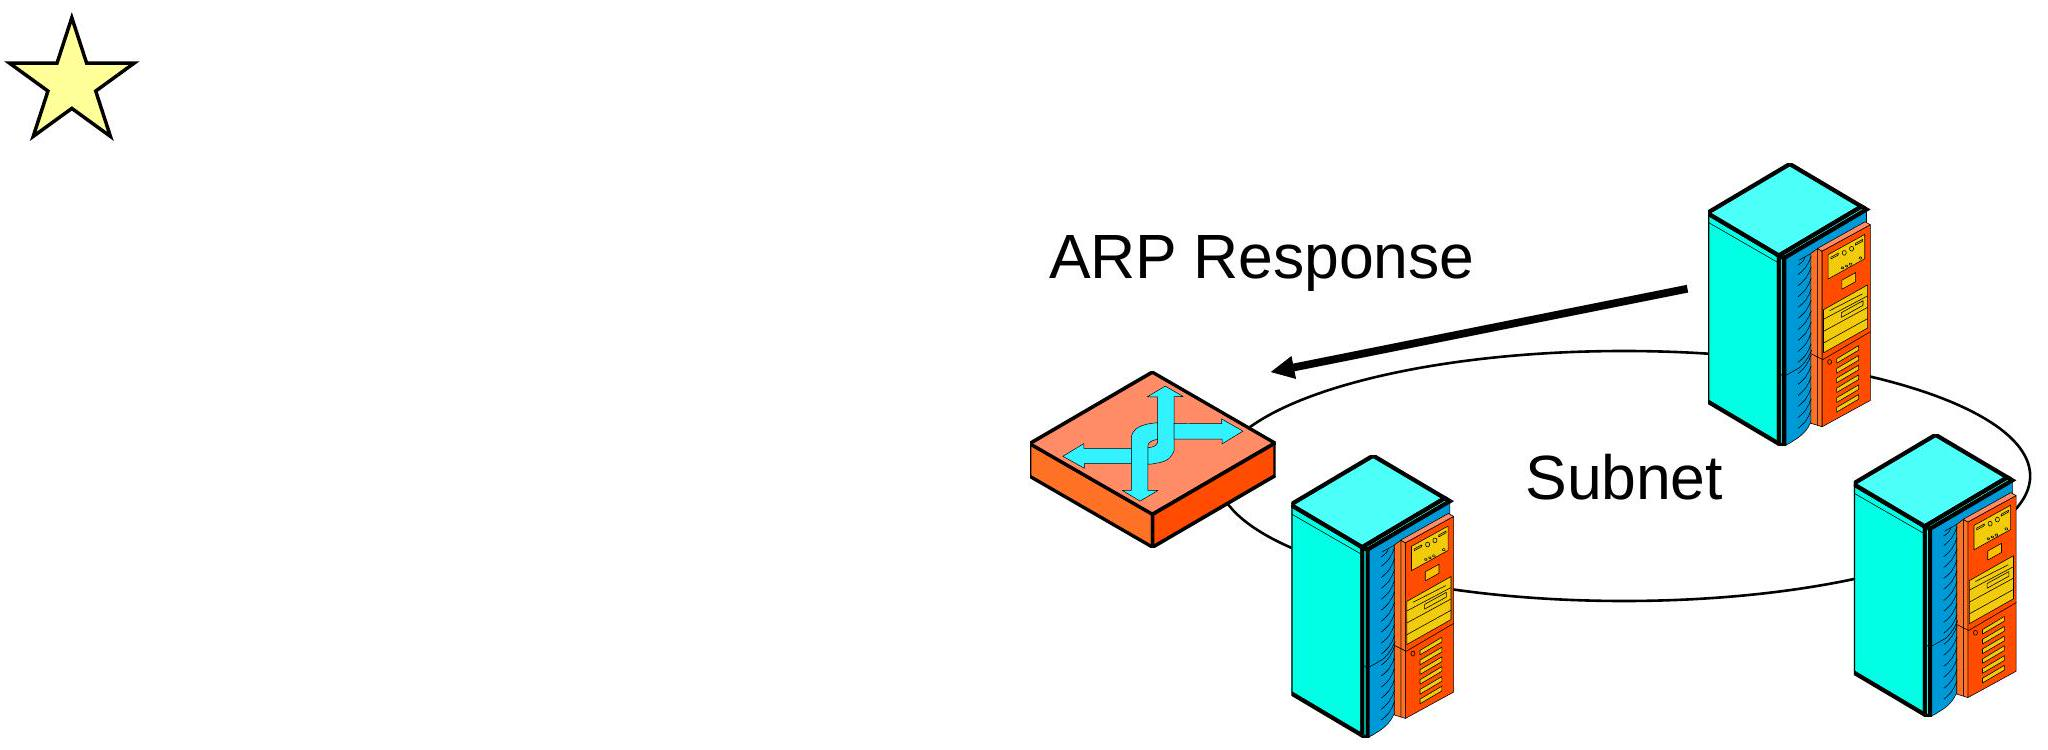
\includegraphics[max width=\textwidth, center]{2023_01_13_b07e3b4bcffdaab9792bg-172}

\end{itemize}

\section*{Address Resolution Protocol }
\begin{itemize}
  \item Router delivers the IP packet to the destination host
\end{itemize}

o Places the IP packet in the subnet frame

o Puts the destination host's subnet address in the destination address field of the frame

\begin{center}
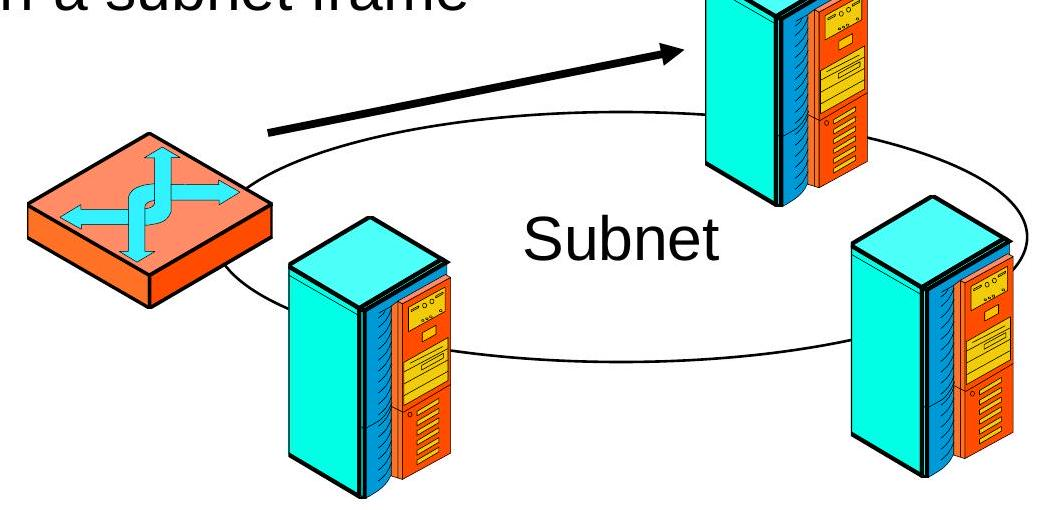
\includegraphics[max width=\textwidth]{2023_01_13_b07e3b4bcffdaab9792bg-173}
\end{center}

\section{Address Resolution Protocol}
\begin{itemize}
  \item ARP Requests and Responses are sent between thr
internet layer processes on the router and the
destination host
\end{itemize}

Router

\begin{center}
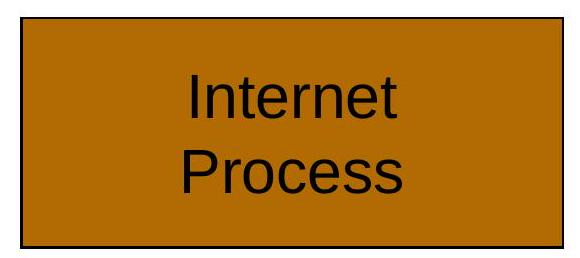
\includegraphics[max width=\textwidth]{2023_01_13_b07e3b4bcffdaab9792bg-174}
\end{center}

ARP

Request

\begin{center}
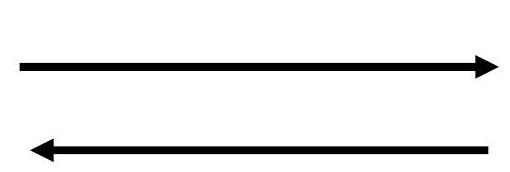
\includegraphics[max width=\textwidth]{2023_01_13_b07e3b4bcffdaab9792bg-174(1)}
\end{center}

ARP

Response Destination Host

Internet
Process

\section{Address Resolution Protocol 
 - However, the data link processes deliver these ARP packets 
 o Router broadcasts the ARP Request 
 o Destination host sends ARP response to the subnet source address found in the broadcast frame}
Router

\begin{center}
\begin{tabular}{|c|}
\hline
Internet \\
Process \\
\hline
Data Link \\
Process \\
\hline
\end{tabular}
\end{center}

Broadcast ARP Request

\begin{center}
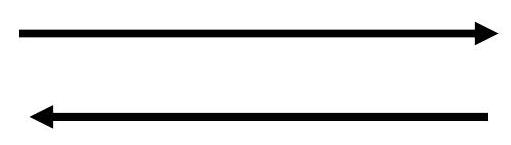
\includegraphics[max width=\textwidth]{2023_01_13_b07e3b4bcffdaab9792bg-175}
\end{center}

Direct ARP Response Destination Host

Data Link

Process

\section*{Direct and Indirect Routing }
\section{- Direct - when nodes are on the same network}
\section{- Indirect - used when the network numbers of the source and destination do not match}


\section{Transmission Control Protocol (TCP)}
\section{TCP: OvervieW RFCs: 793, 1122, 1323, 2018, 2581}
\begin{center}
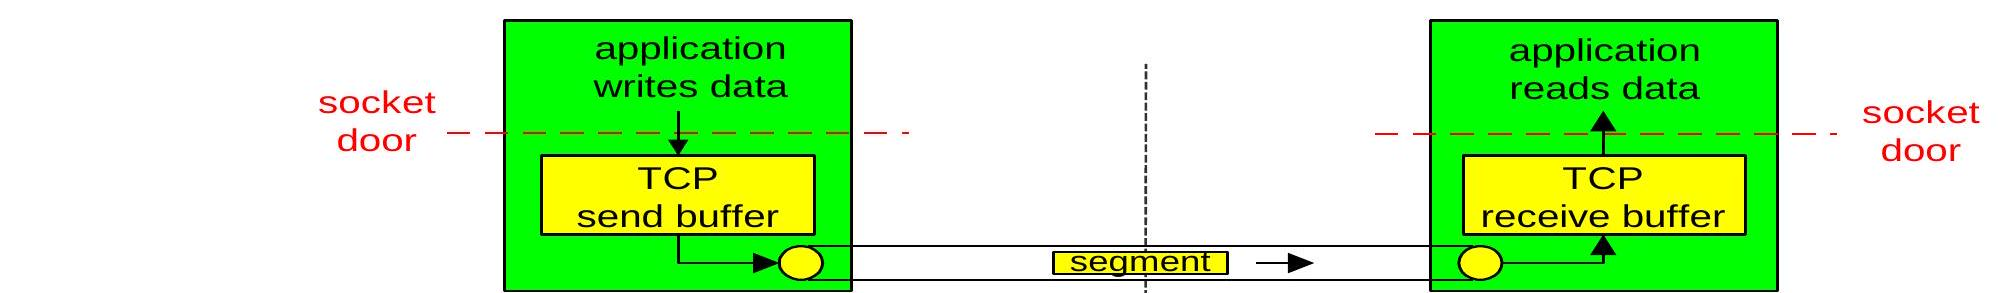
\includegraphics[max width=\textwidth]{2023_01_13_b07e3b4bcffdaab9792bg-178}
\end{center}

\begin{itemize}
  \item point-to-point (unicast):
\end{itemize}

o one sender, one receiver

\begin{itemize}
  \item connection-oriented:

  \item handshaking (exchange of control msgs) init's sender, receiver state before data exchange

  \item State resides only at the END systems - Not a virtual circuit!

  \item full duplex data:

  \item bi-directional data flow in same connection (A->B \& B->A in the same connection)

\end{itemize}

o MSS: maximum segment size - reliable, in-order byte steam: o no "message boundaries"

\begin{itemize}
  \item send \& receive buffers o buffer incoming \& outgoing data

  \item flow controlled:

\end{itemize}

o sender will not overwhelm receiver

\begin{itemize}
  \item congestion controlled:
\end{itemize}

o sender will not overwhelm network

\section{TCP segment structure}
\section{2 bits}
URG: urgent data (generally not used)

ACK: ACK \# valid

PSH: push data now (generally not used)

RST, SYN, FIN: connection estab (setup, teardown commands)

Internet checksum (as in UDP)
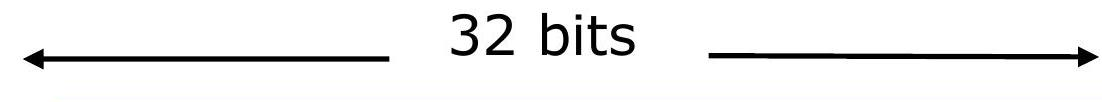
\includegraphics[max width=\textwidth, center]{2023_01_13_b07e3b4bcffdaab9792bg-179}

\begin{center}
\begin{tabular}{|c|c|}
\hline
source port \# & dest port \# \\
\hline
\end{tabular}
\end{center}

by bytes

of data

(not segments!)

$$
\begin{aligned}
& \text { application } \\
& \text { data } \\
& \text { (variable length) }
\end{aligned}
$$

\# bytes

rcvr willing

to accept

\section{TCP Connection-oriented demux}
\begin{itemize}
  \item TCP socket identified by 4 -tuple:
\end{itemize}

o source IP address

o source port number

o dest IP address

o dest port number

\section{- receiving host uses all four values to direct segment to appropriate socket}
\section{TCP Demultiplexing Example}
\begin{center}
\begin{tabular}{|l|l|l|l|l|l|}
\hline
 &  &  &  \\
\hline
\end{tabular}
\end{center}

\section{Typical TCP Transaction}
\begin{center}
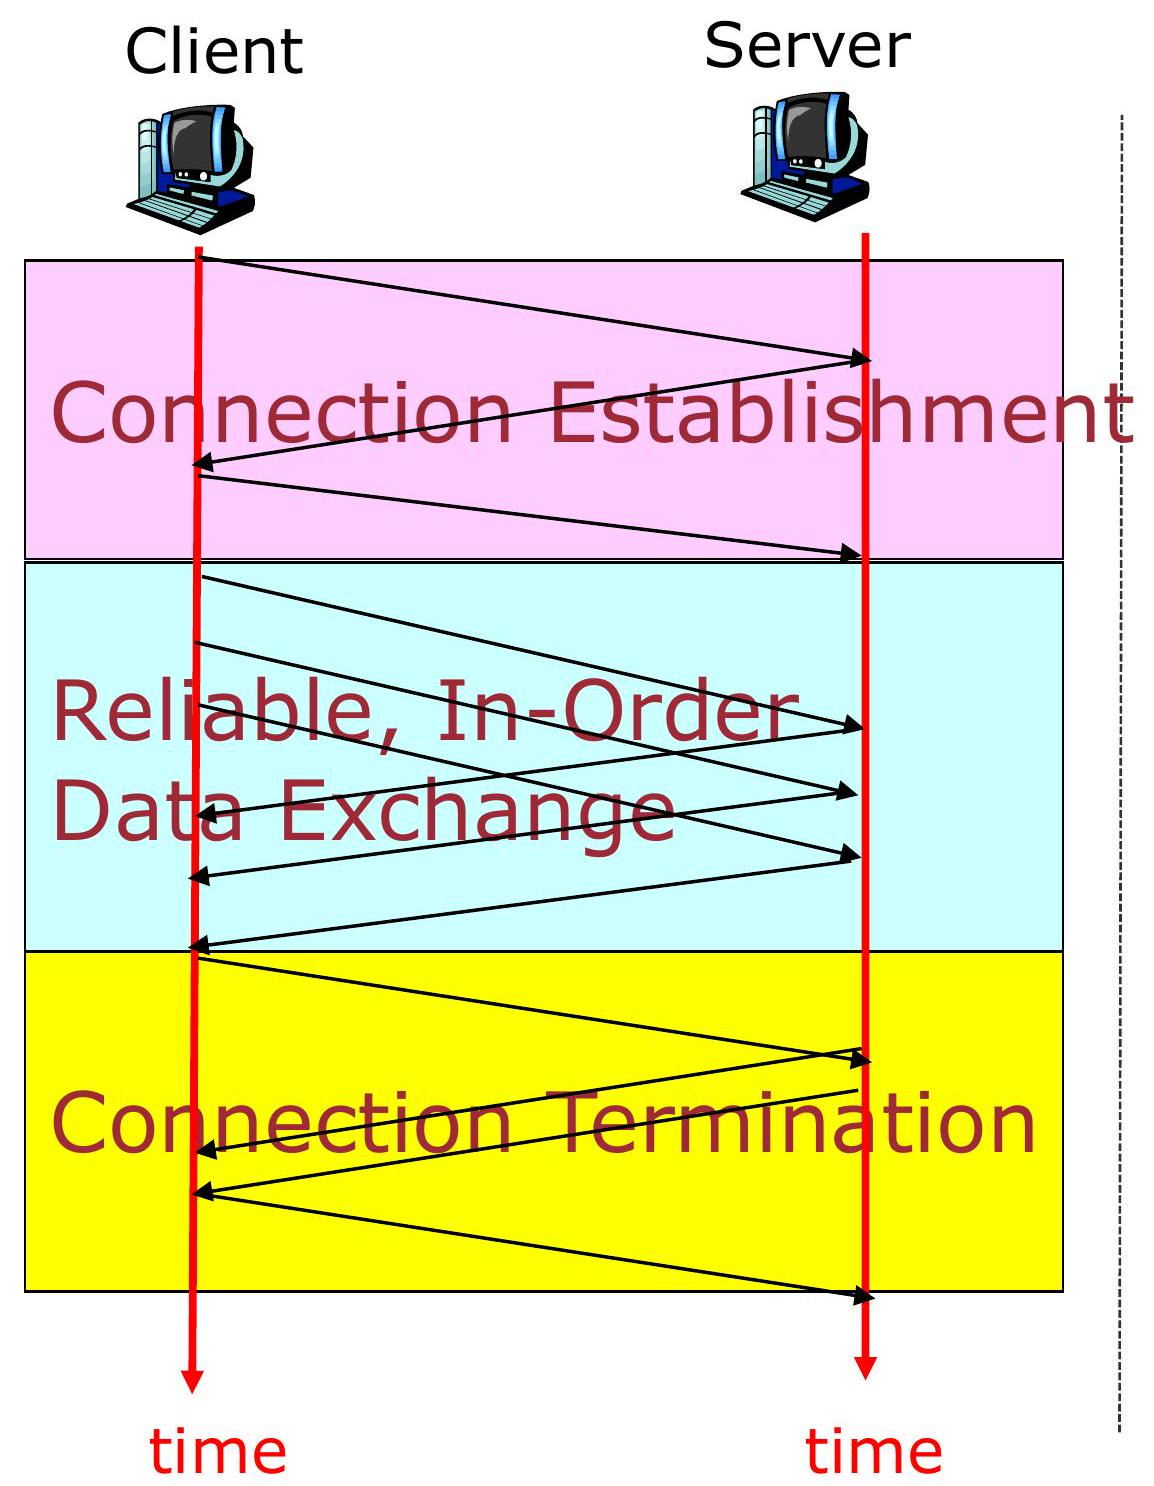
\includegraphics[max width=\textwidth]{2023_01_13_b07e3b4bcffdaab9792bg-182}
\end{center}

\section{A TCP Transaction consists of 3 Phases}
\begin{enumerate}
  \item Connection Establishment
\end{enumerate}

o Handshaking between client and server

\section{Reliable, In-Order Data Exchange}
o Recover any lost data through retransmissions and ACKs

\section{Connection Termination o Closing the connection}
\section{TCP Connection Establishment}
\begin{itemize}
  \item TCP sender, receiver establish "connection" before exchanging data segments

  \item initialize TCP variables:

\end{itemize}

o seq. \#s

o buffers, flow control info (e.g. RcvWindow)

\begin{itemize}
  \item client: connection initiator
\end{itemize}

Socket clientSocket $=$ new Socket ("hostname", port\#);

\begin{itemize}
  \item server: contacted by client Socket connectionSocket $=$ welcomeSocket. accept () ;
\end{itemize}

\section{Connection Establishment (cont)}
\section{Three way handshake:}
Step 1: client host sends TCP SYN segment to server

o specifies a random initial seq \#

o no data

Step 2: server host receives SYN, replies with SYNACK segment o server allocates buffers

o specifies server initial seq. \# Step 3: client receives SYNACK, replies with $\mathrm{ACK}$ segment, which may contain data

\begin{center}
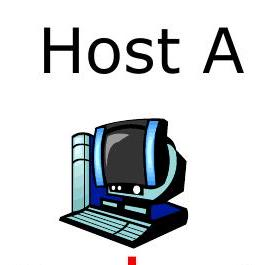
\includegraphics[max width=\textwidth]{2023_01_13_b07e3b4bcffdaab9792bg-184}
\end{center}

Host B

Conhection

request $\sqrt{S Y N, S_{e q}=42} \quad$ host ACKs and selects its own initial seq \#

\section{Connection Establishment (cont)}
\section{Seq. \#'s:}
o byte stream "number" of first byte in segment's data

\section{ACKs:}
O seq \# of next byte expected from other side

o cumulative ACK

\begin{center}

\includegraphics[max width=\textwidth]{2023_01_13_b07e3b4bcffdaab9792bg-185}
\end{center}

Host B

Connection

request

\begin{center}
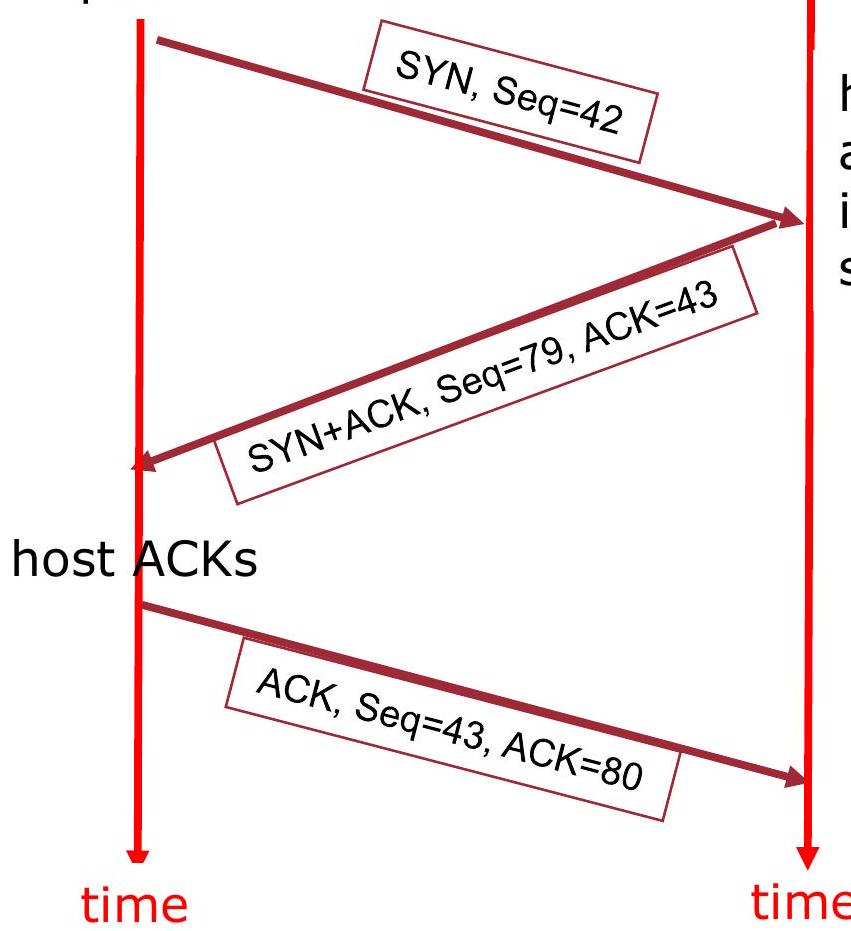
\includegraphics[max width=\textwidth]{2023_01_13_b07e3b4bcffdaab9792bg-185(1)}
\end{center}

host ACKs and selects its own initial seq \#

Three-way handshake

\section{TCP Starting Sequence Number Selection}
\begin{itemize}
  \item Why a random starting sequence \#? Why not simply choose o?

  \item To protect against two incarnations of the same connection reusing the same sequence numbers too soon

  \item That is, while there is still a chance that a segment from an earlier incarnation of a connection will interfere with a later incarnation of the connection

  \item How?

  \item Client machine seq \#o, initiates connection to server with seq \#0.

  \item Client sends one byte and client machine crashes

  \item Client reboots and initiates connection again

  \item Server thinks new incarnation is the same as old connection

\end{itemize}

\section{TCP Connection Termination}
\section{Closing a connection:}
client closes socket:

clientSocket. close () ;

\section{Step 1: client end system sends TCP FIN control segment to server}
Step 2: server receives FIN, replies with $\mathrm{ACK}$. Server might send some buffered but not sent data before closing the connection. Server then sends FIN and moves to Closing state.

\begin{center}
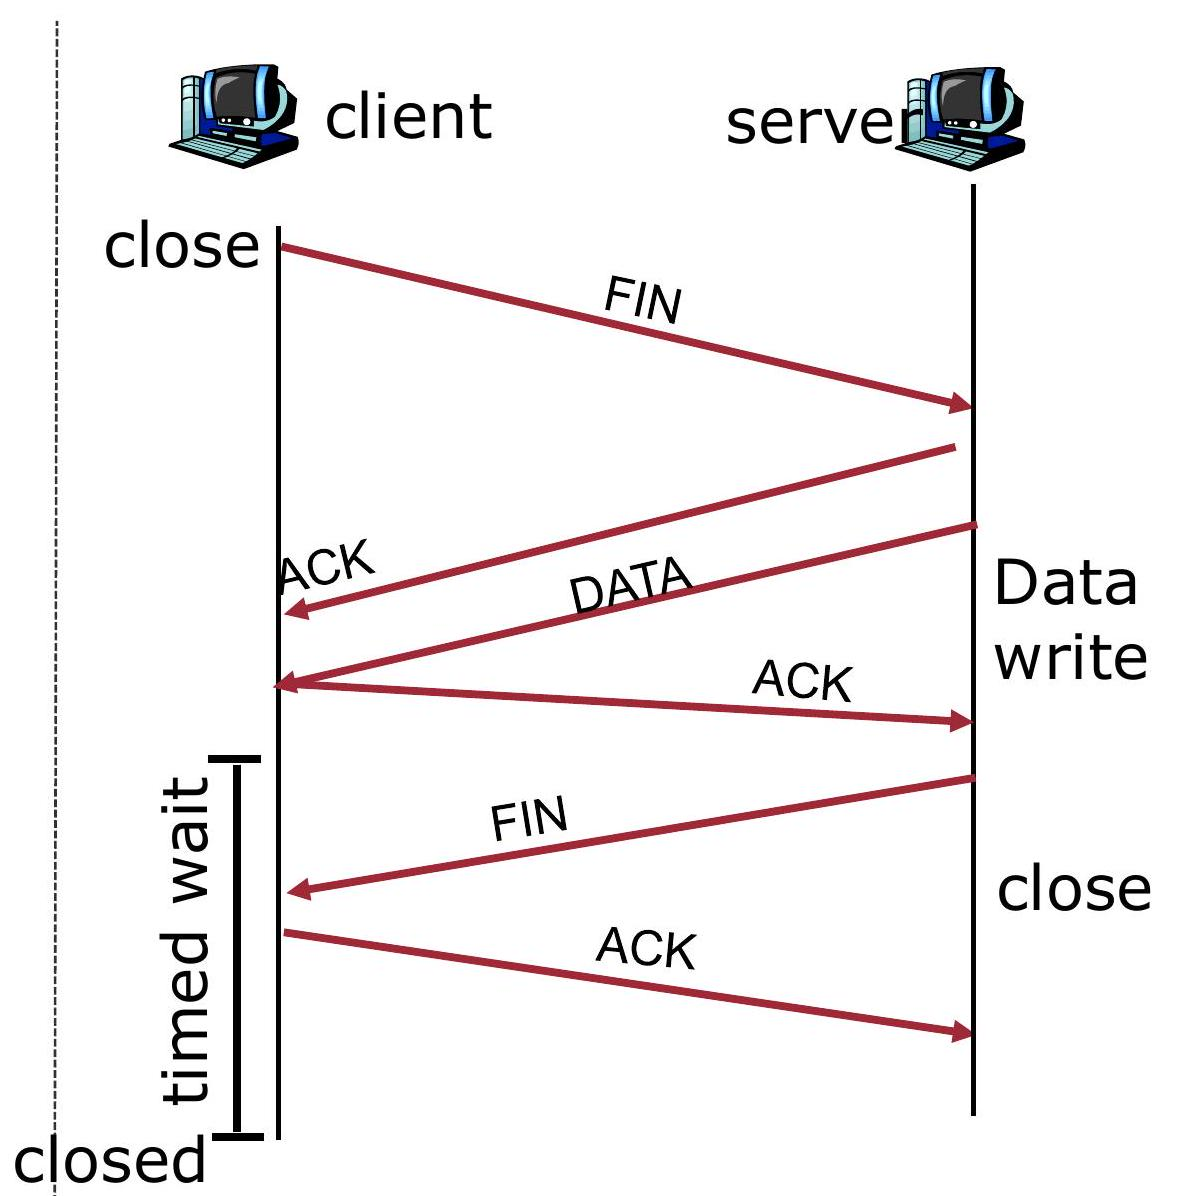
\includegraphics[max width=\textwidth]{2023_01_13_b07e3b4bcffdaab9792bg-187}
\end{center}

\section{TCP Connection Termination}
Step 3: client receives FIN, replies with ACK.

o Enters "timed wait" - will respond with ACK to received FINs

Step 4: server, receives ACK. Connection closed.

\begin{itemize}
  \item Why wait before closing the connection?

  \item If the connection were allowed to move to CLOSED state, then another pair of application processes might come along and open the same connection (use the same port \#s) and a delayed FIN from an earlier incarnation would terminate the connection.

\end{itemize}

\begin{center}
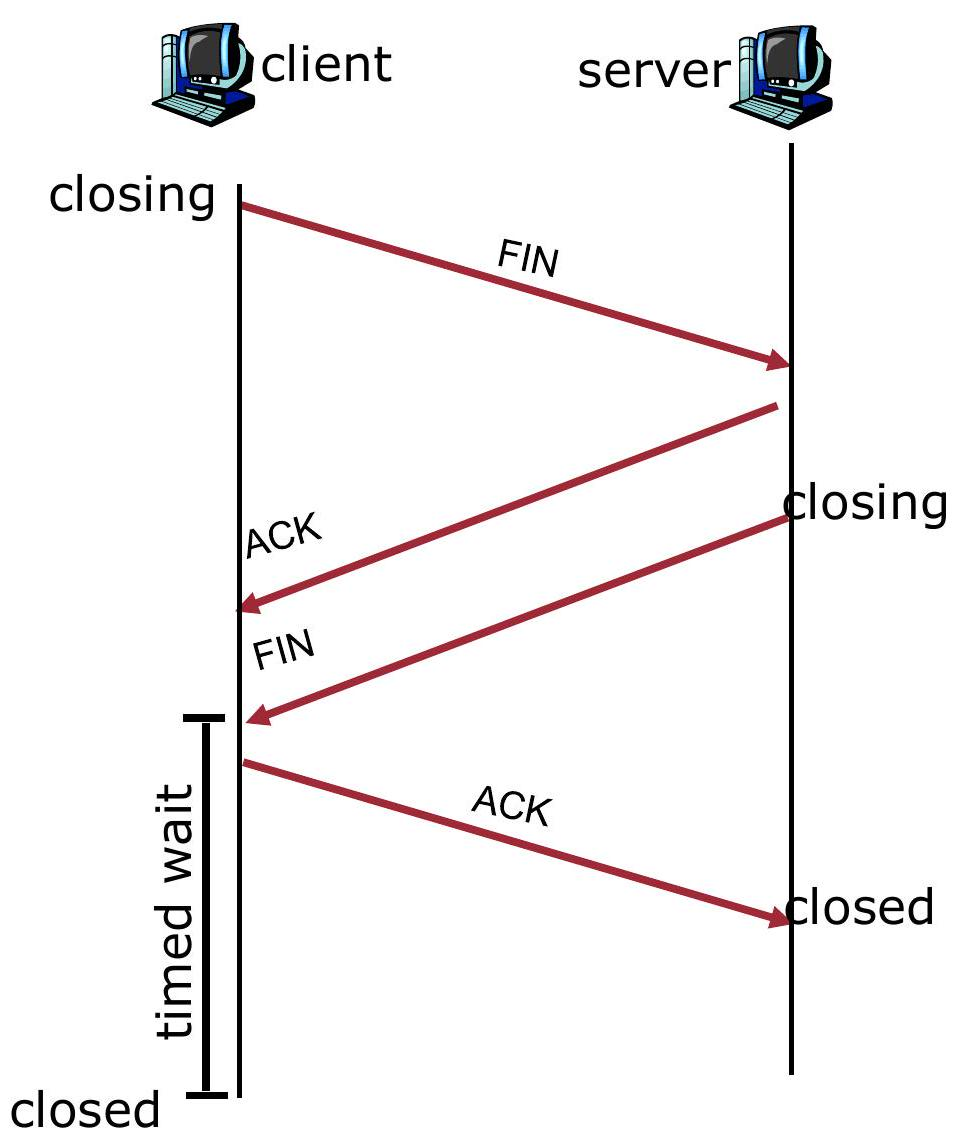
\includegraphics[max width=\textwidth]{2023_01_13_b07e3b4bcffdaab9792bg-188}
\end{center}

\section{TCP State-Transition Diagram}
\begin{center}
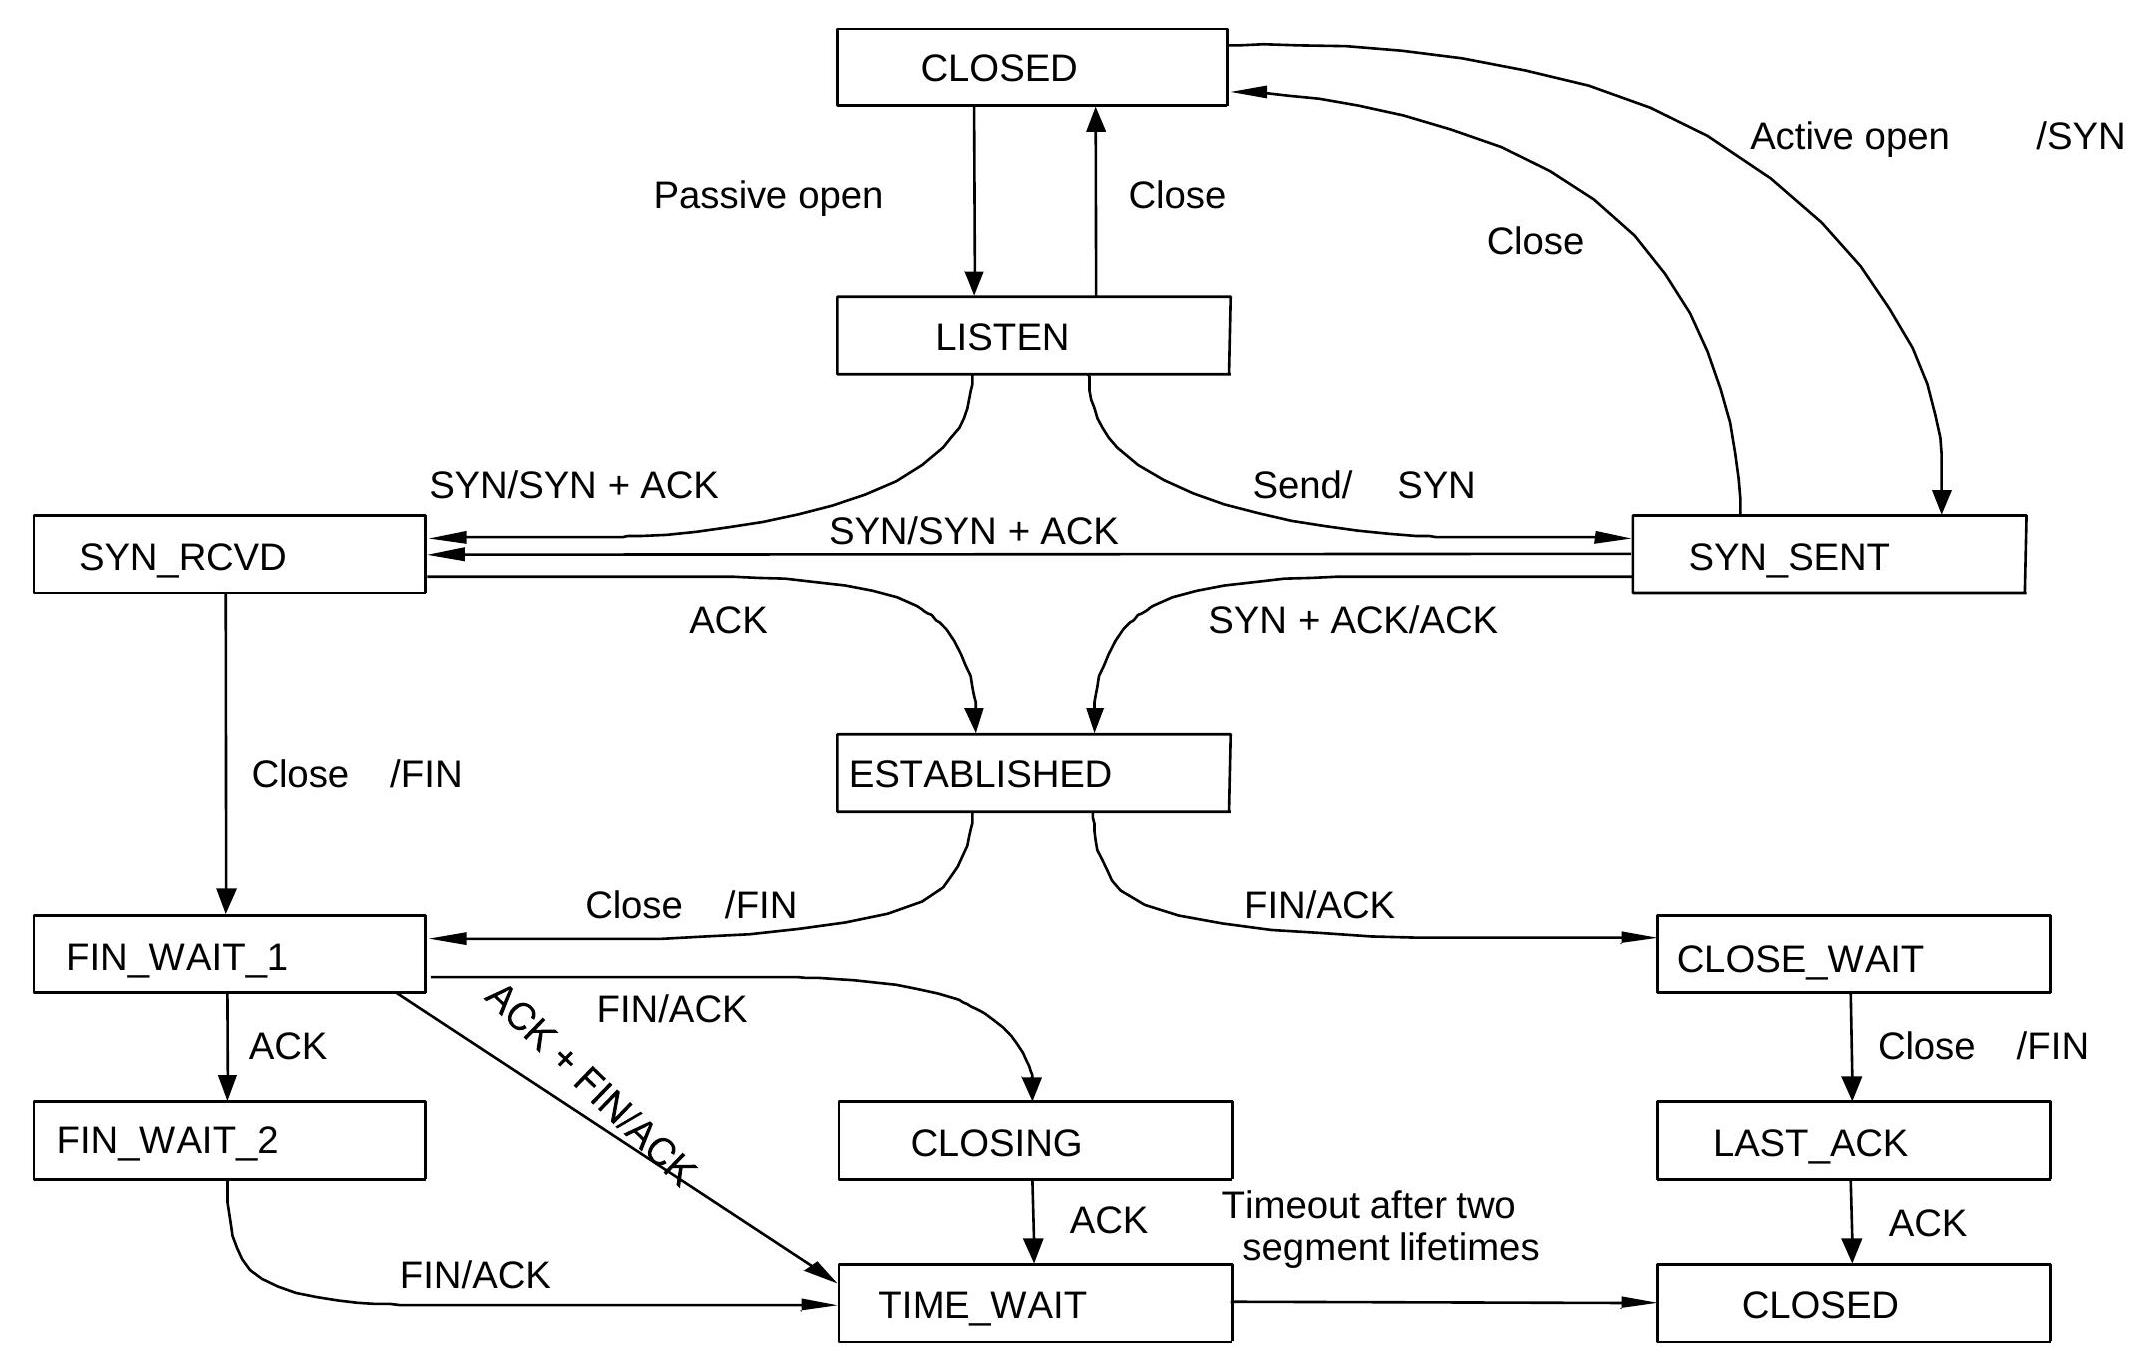
\includegraphics[max width=\textwidth]{2023_01_13_b07e3b4bcffdaab9792bg-189}
\end{center}

\section{Typical TCP Client/Server Transitions}
\begin{center}
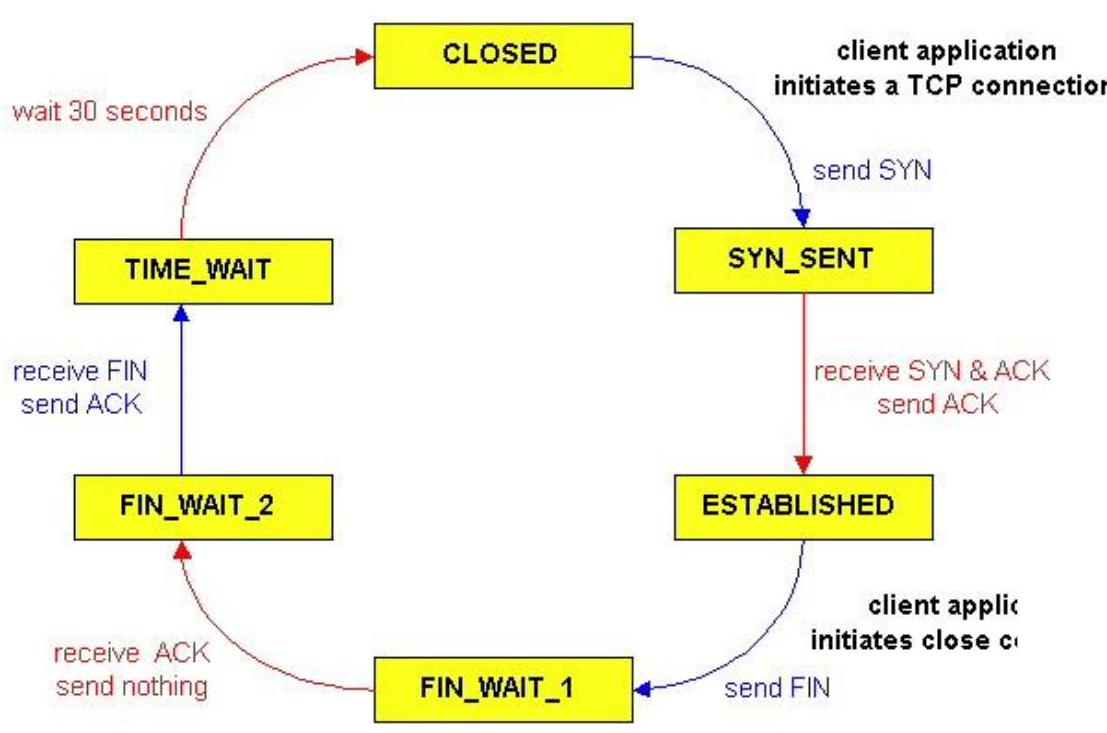
\includegraphics[max width=\textwidth]{2023_01_13_b07e3b4bcffdaab9792bg-190}
\end{center}

TCP client

lifecycle TCP server lifecycle

\begin{center}
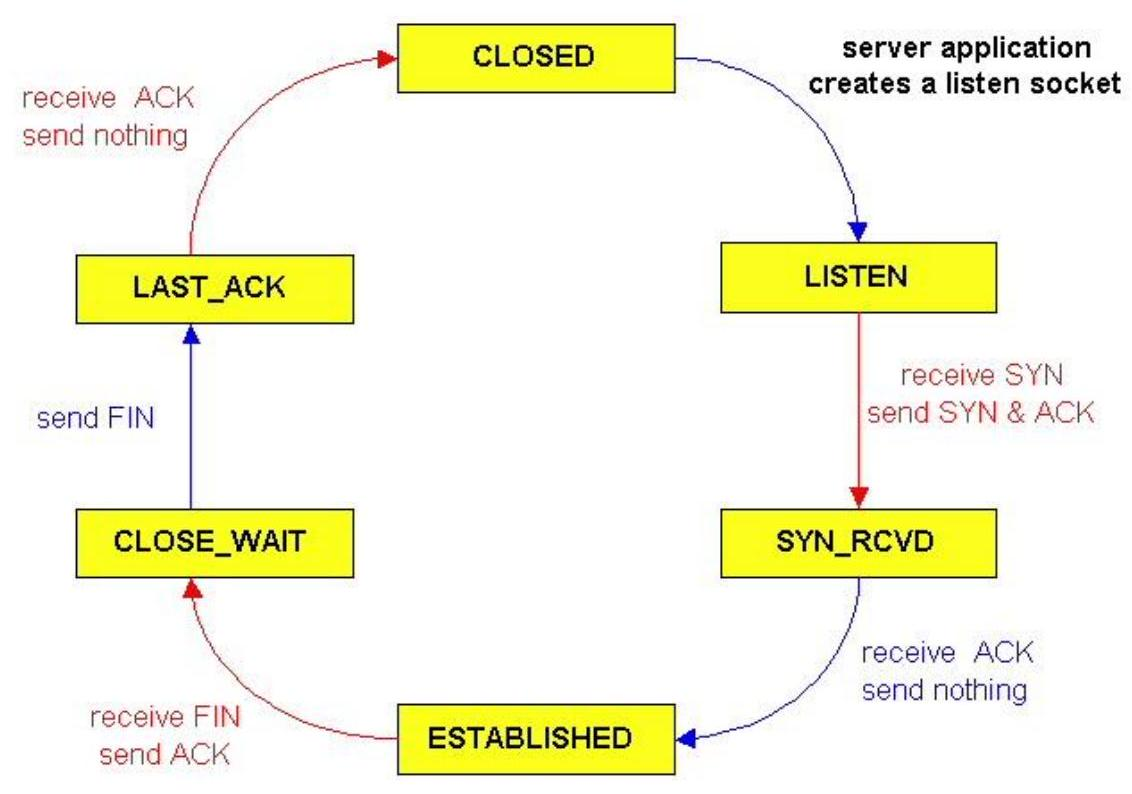
\includegraphics[max width=\textwidth]{2023_01_13_b07e3b4bcffdaab9792bg-190(1)}
\end{center}

\section{How to program using the TCP?}
\begin{center}
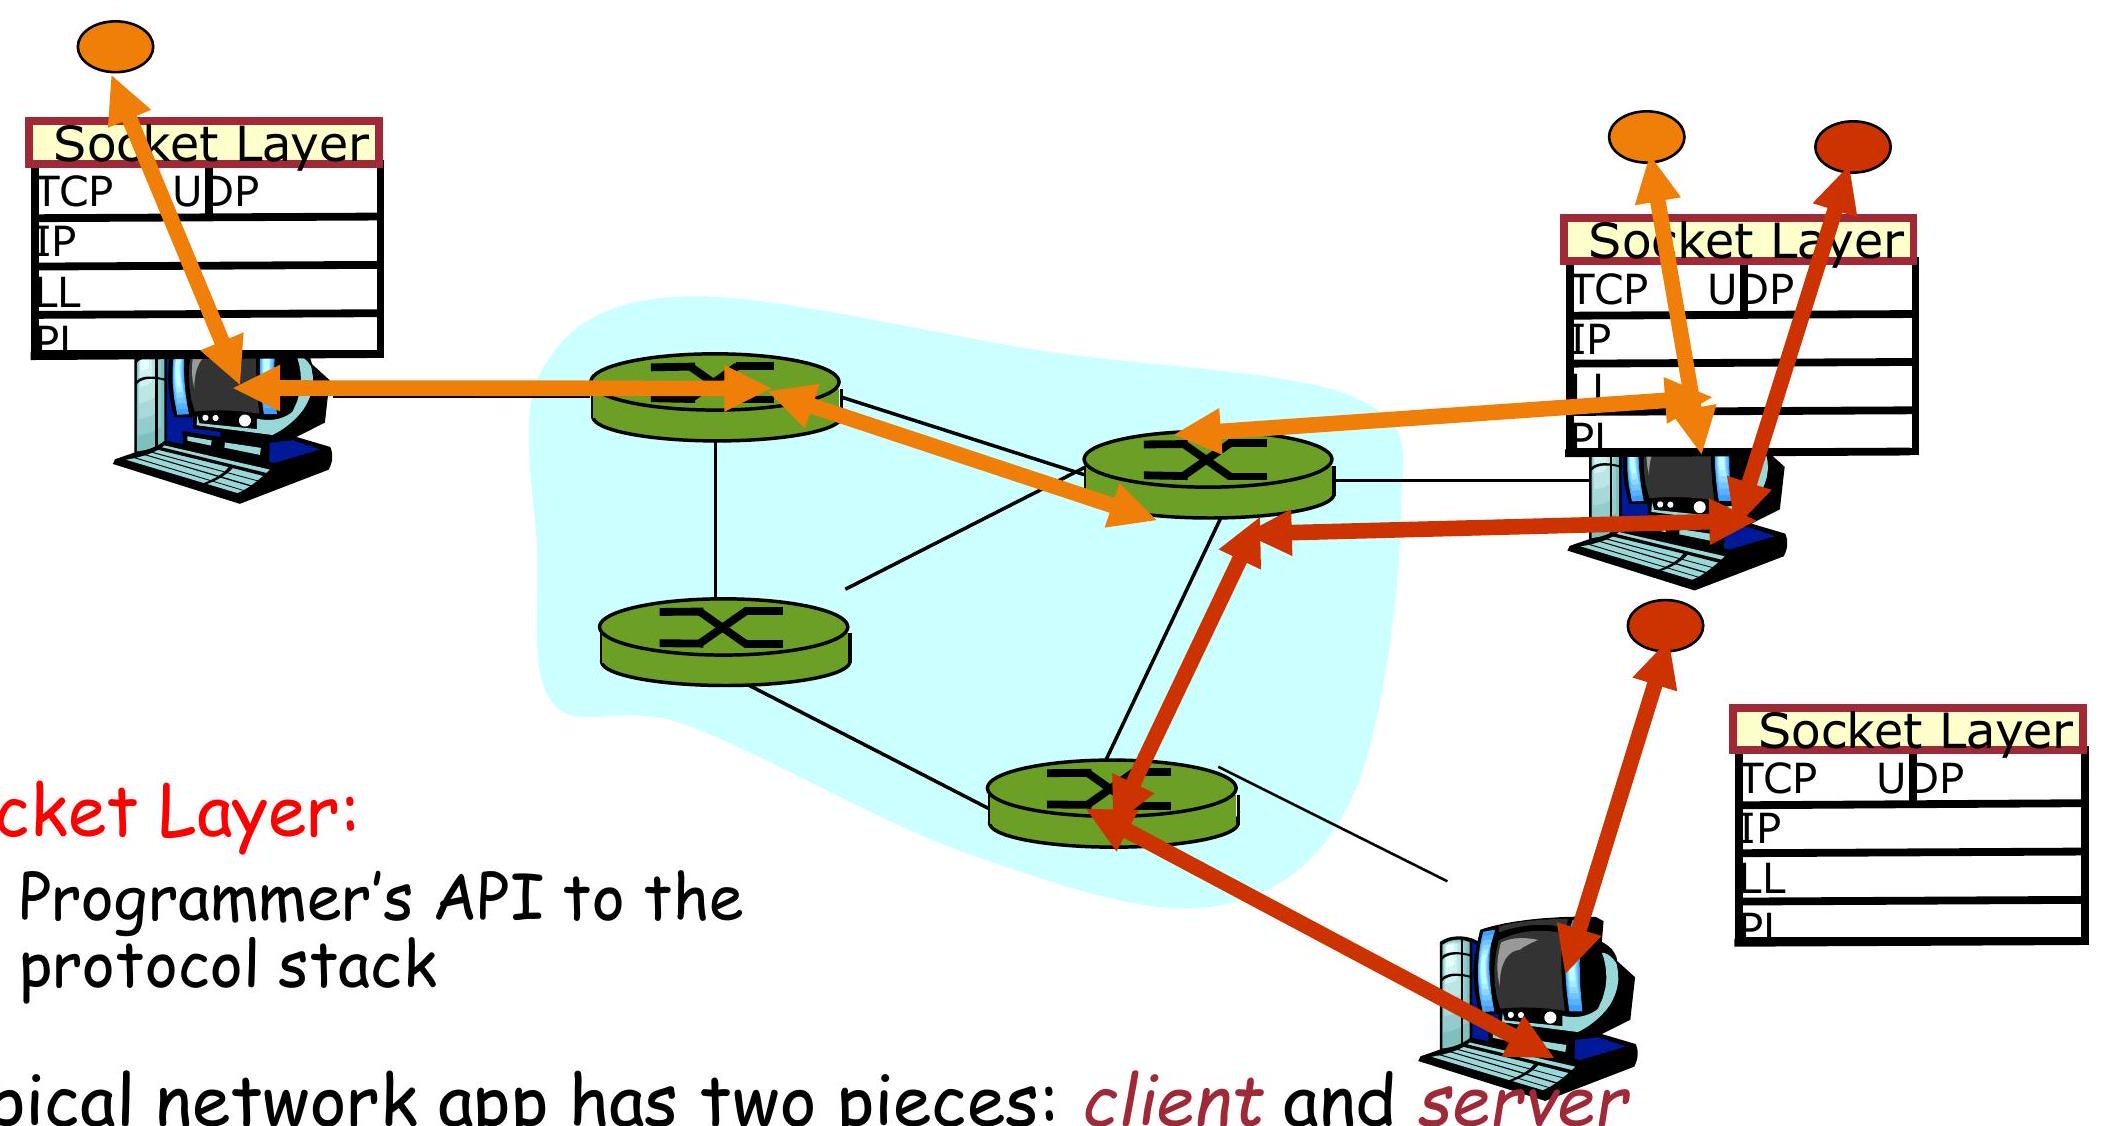
\includegraphics[max width=\textwidth]{2023_01_13_b07e3b4bcffdaab9792bg-191}
\end{center}

o Programmer's API to the protocol stack

$\square$ Typical network app has two pieces: client and server Server: Passive entity. Provides service to clients

o e.g., Web server responds with the requested Web page

$\square$ Client: initiates contact with server ("speaks first")

o typically requests service from server, e.9., Web Browser

\section{Socket Creation}
\begin{itemize}
  \item mySock = socket(family, type, protocol);

  \item UDP/TCP/IP-specific sockets

\end{itemize}

\begin{center}
\begin{tabular}{|l|c|c|l|}
\multicolumn{2}{c}{Family} & Type & Protocol \\
\hline
TCP & \multirow{3}{*}{PF\_INET} & SOCK\_STREAM & IPPROTO\_TCP \\
\cline { 3 - 4 }
 &  & SOCK\_DGRAM & IPPROTO\_UDP \\
\hline
UDP &  &  &  \\
\hline
\end{tabular}
\end{center}

\begin{itemize}
  \item Socket reference
\end{itemize}

o File (socket) descriptor in UNIX

o Socket handle in WinSock

\section{TCP Client/Server Interaction}
Server starts by getting ready to receive client connections...



\begin{enumerate}
  \item Create a TCP socket

  \item Establish connection

  \item Communicate

  \item Close the connection Server

\end{enumerate}

Create a TCP socket

Assign a port to socket

Set socket to listen

Repeatedly:

a. Accept new connection

b. Communicate

c. Close the connection

\section{TCP Client/Server Interaction}
$/ *$ Create socket for incoming connections */

if $(($ servSock $=$ socket(PF\_INET, SOCK\_STREAM, IPPROTO\_TCP $))<0)$ DieWithError("socket() failed");

Client

\begin{enumerate}
  \item Create a TCP socket

  \item Establish connection

  \item Communicate

  \item Close the connection Server

\end{enumerate}

Create a TCP socket

Bind socket to a port

Set socket to listen

Repeatedly:

a. Accept new connection

b. Communicate

c. Close the connection

\section{TCP Client/Server Interaction}
echoServAddr.sin\_family $=$ AF\_INET;

echoServAddr.sin\_addr.s\_addr $=$ htonl(INADDR\_ANY);/* Any incoming interface */ echoServAddr.sin\_port $=$ htons(echoServPort);

if (bind(servSock, (struct sockaddr DieWithError("bind() failed");

\section{Client}
\begin{enumerate}
  \item $\quad$ Create a TCP socket

  \item Establish connection

  \item Communicate

  \item Close the connection /* Internet address family \textit{/ /} Local port */

\end{enumerate}

Server

Create a TCP socket Bind socket to a port

Set socket to listen

Repeatedly:
a. Accept new connection
b. Communicate
c. Close the connection

\section*{TCP Client/Server Interaction }
Client

\begin{enumerate}
  \item Create a TCP socket

  \item Establish connection

  \item Communicate

  \item Close the connection Server

\end{enumerate}

Create a TCP socket Bind socket to a port

Set socket to listen

Repeatedly:
a. Accept new connection
b. Communicate
c. Close the connection

\section*{TCP Client/Server Interaction }
\textbackslash author\{
for $(i ;) / *$ Run forever $* /$ \textbackslash  \{ \textbackslash  clntLen $=$ sizeof(echoCIntAddr $)$; \textbackslash  if $(($ clntSock=accept(servSock, (struct sockaddr * $)$ \&echoCIntAddr, \&clntLen $))<0)$ \textbackslash  DieWithError("accept() failed");
\}

\section{Client}
\begin{enumerate}
  \item Create a TCP socket

  \item Establish connection

  \item Communicate

  \item Close the connection

\end{enumerate}

\section{Server}
Create a TCP socket Bind socket to a port Set socket to listen Repeatedly:
a. Accept new connection
b. Communicate
c. Close the connection

\section{TCP Client/Server Interaction}
Server is now blocked waiting for connection from a client



\begin{enumerate}
  \item Create a TCP socket

  \item Establish connection

  \item Communicate

  \item Close the connection

\end{enumerate}

\section{Server}
Create a TCP socket

Bind socket to a port

Set socket to listen

Repeatedly:
a. Accept new connection
b. Communicate
c. Close the connection

\section{TCP Client/Server Interaction}
Later, a client decides to talk to the server...



\begin{enumerate}
  \item Create a TCP socket

  \item Establish connection

  \item Communicate

  \item Close the connection Server

\end{enumerate}

Create a TCP socket

Bind socket to a port

Set socket to listen

Repeatedly:
a. Accept new connection
b. Communicate
c. Close the connection

\section{TCP Client/Server Interaction}
/* Create a reliable, stream socket using TCP */

if $(($ sock $=$ socket(PF\_INET, SOCK\_STREAM, IPPROTO\_TCP $))<0)$ DieWithError("socket() failed");

\section{Client}
\begin{enumerate}
  \item Create a TCP socket

  \item Establish connection

  \item Communicate

  \item Close the connection Server

\end{enumerate}

Create a TCP socket Bind socket to a port

Set socket to listen Repeatedly:

a. Accept new connection

b. Communicate

c. Close the connection

\section*{TCP Client/Server Interaction }
Client

\begin{enumerate}
  \item Create a TCP socket

  \item Establish connection

  \item Communicate

  \item Close the connection

\end{enumerate}

\section{Server}
Create a TCP socket

Bind socket to a port

Set socket to listen

Repeatedly:
a. Accept new connection
b. Communicate
c. Close the connection

\section{TCP Client/Server Interaction}
echoStringLen $=$ strlen $($ echoString $)$;

/* Determine input length * /

/* Send the string to the server $* /$

if (send(sock, echoString, echoStringLen, 0) $!=$ echoStringLen)

DieWithError("send() sent a different number of bytes than expected");

Client

\begin{enumerate}
  \item Create a TCP socket

  \item Establish connection

  \item Communicate

  \item Close the connection Server

\end{enumerate}

Create a TCP socket

\begin{enumerate}
  \setcounter{enumi}{1}
  \item Bind socket to a port

  \item Set socket to listen

  \item Repeatedly:

\end{enumerate}

a. Accept new connection

b. Communicate

c. Close the connection

\section{TCP Client/Server Interaction}
/* Receive message from client */

if $(($ recvMsgSize $=\operatorname{recv}($ clntSocket, echoBuffer, RCVBUFSIZE, 0) $)<0)$ DieWithError("recv() failed");

Client

\begin{enumerate}
  \item Create a TCP socket

  \item Establish connection

  \item Communicate

  \item Close the connection Server

  \item Create a TCP socket

\end{enumerate}

. Bind socket to a port

\begin{enumerate}
  \setcounter{enumi}{2}
  \item Set socket to listen

  \item Repeatedly:
a. Accept new connection
b. Communicate
c. Close the connection

\end{enumerate}

\section{TCP Client/Server Interaction}
close(sock);



\begin{enumerate}
  \item Create a TCP socket

  \item Establish connection

  \item Communicate

  \item Close the connection

\end{enumerate}

\section{close(clntSocket)}
Server

Create a TCP socket

Bind socket to a port

Set socket to listen

Repeatedly:

a. Accept new connection

b. Communicate

c. Close the connection

\section*{TCP Tidbits }
\begin{itemize}
  \item Client knows server address and port

  \item No correlation between send () and recv ()

\end{itemize}

Server

$\operatorname{recv}()->$ "Hello"

$\operatorname{recv}()->$ "Bob"

send("Hi ")

send("Jane")

$\operatorname{recv}()->$ "Hi Jane"

\section{Serial Busses}
\begin{center}
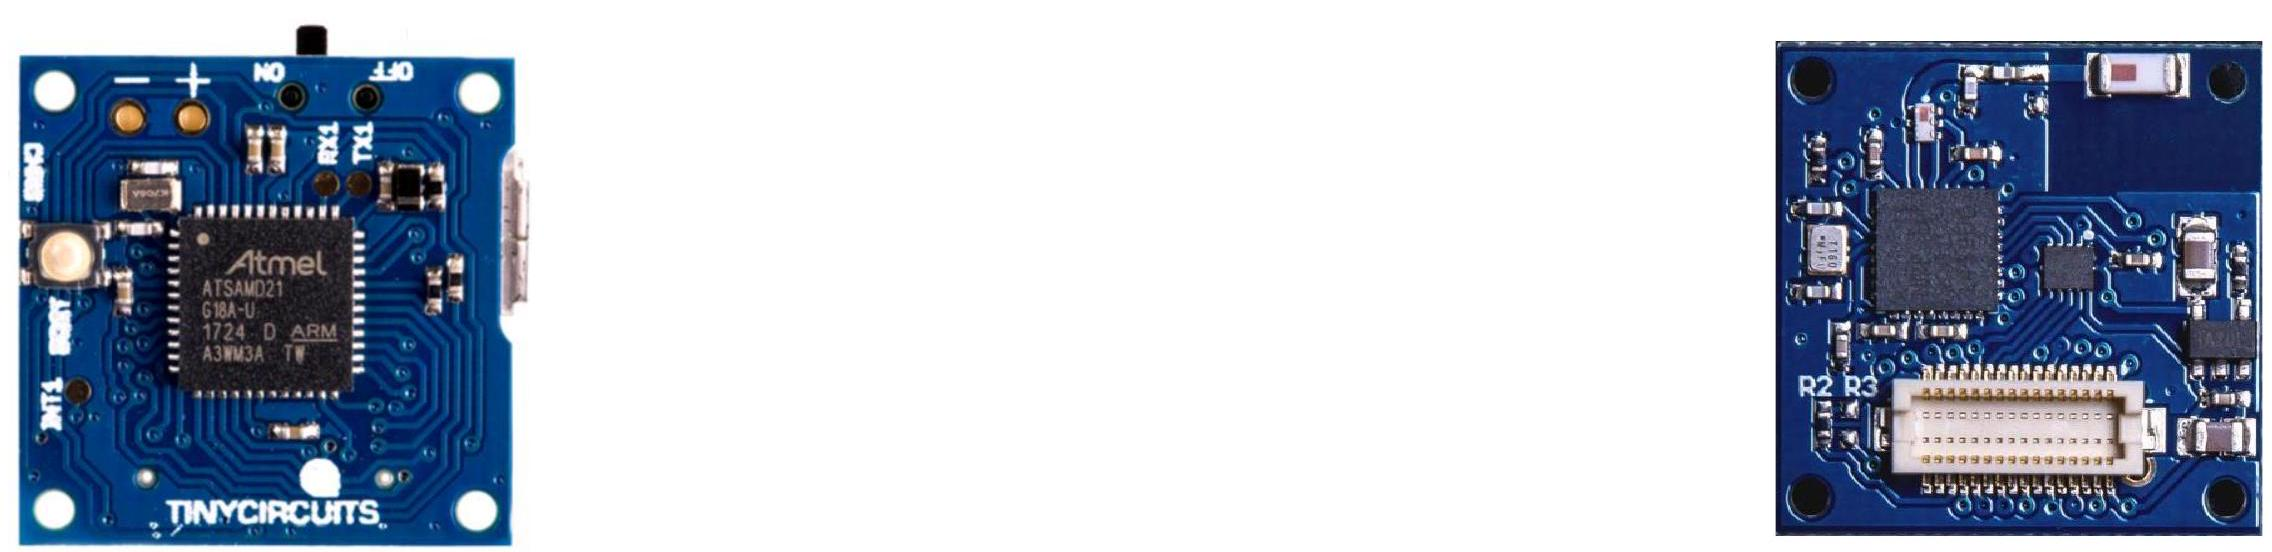
\includegraphics[max width=\textwidth]{2023_01_13_b07e3b4bcffdaab9792bg-206}
\end{center}

\section{Serial Buses in Embedded}
\begin{itemize}
  \item UART serial bus for sending debug messages to your
development host

  \item I2C serial bus for communicating with sensors (e.g., the accelerometer)

\end{itemize}

\section{- SPI serial bus for communicating with the Bluetooth Low Energy radio}
\section{Serial Interfaces}
\begin{center}
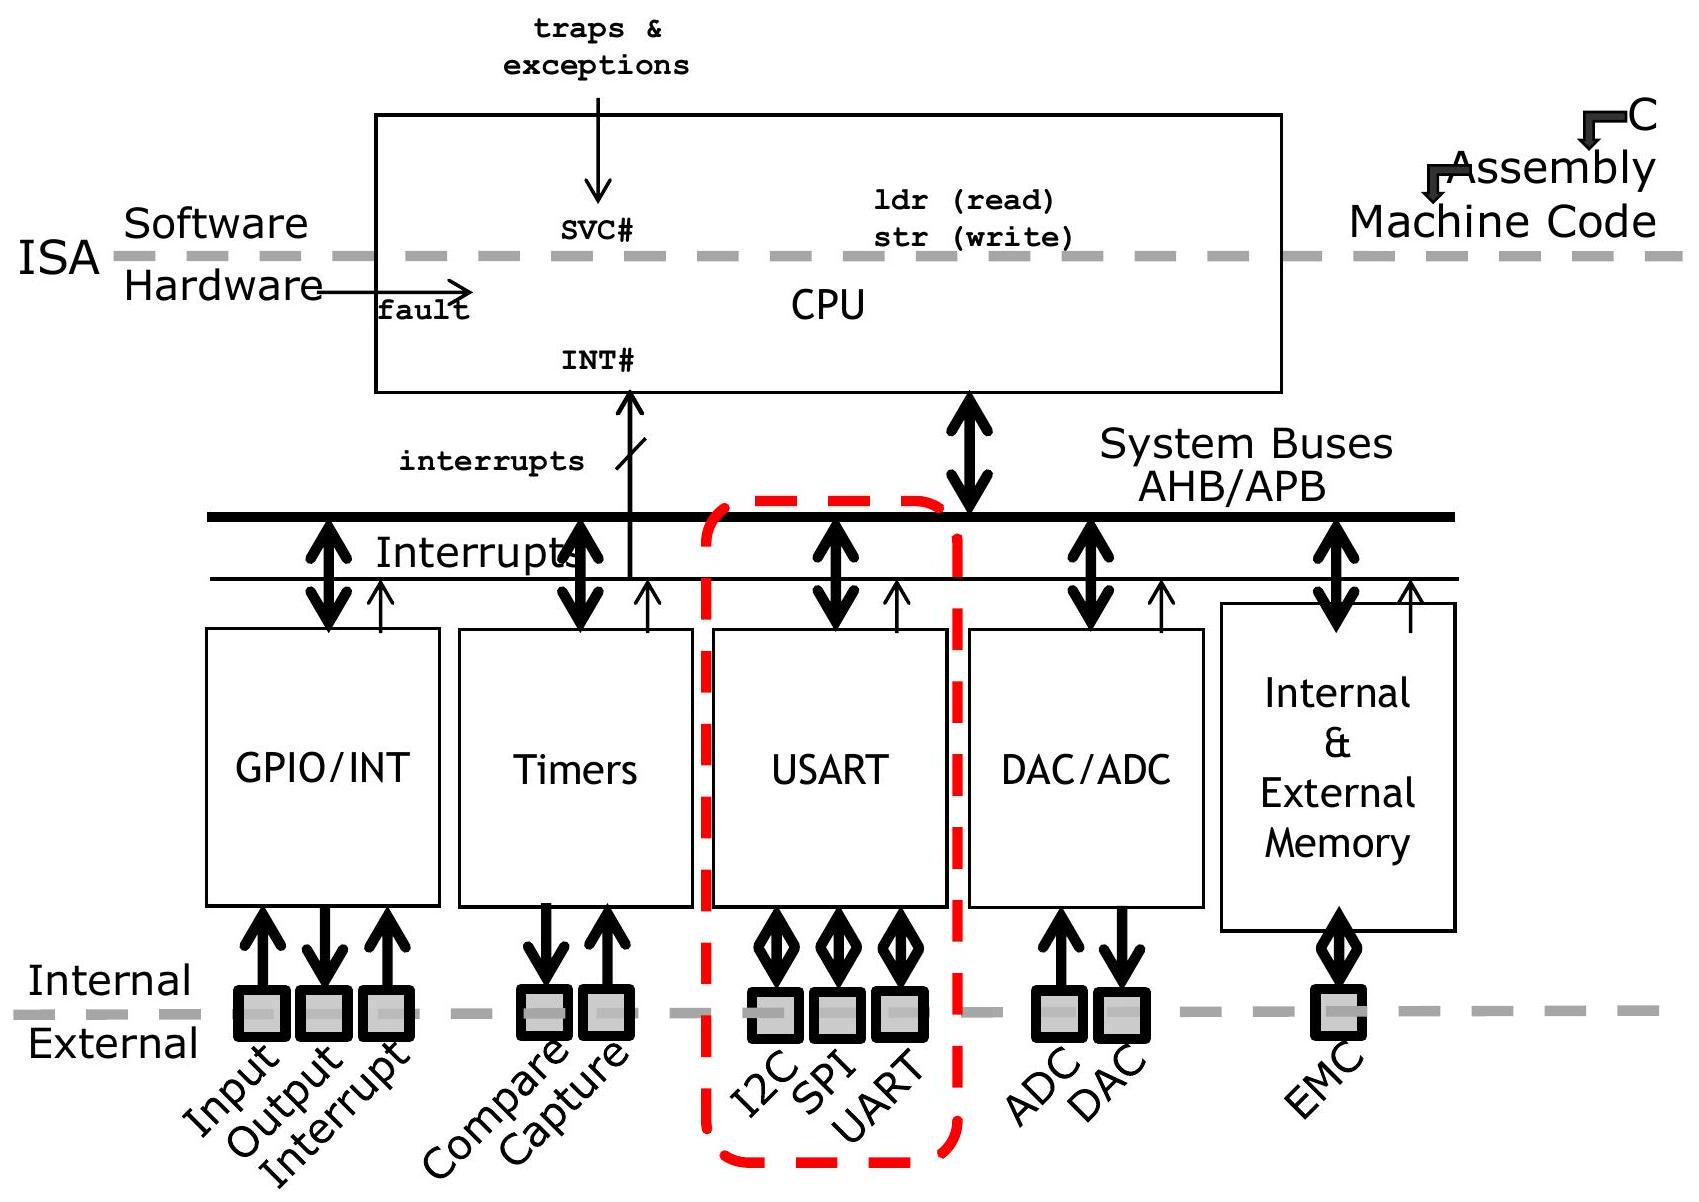
\includegraphics[max width=\textwidth]{2023_01_13_b07e3b4bcffdaab9792bg-208}
\end{center}

\section{Parallel Bus VS Serial Bus}
\begin{center}
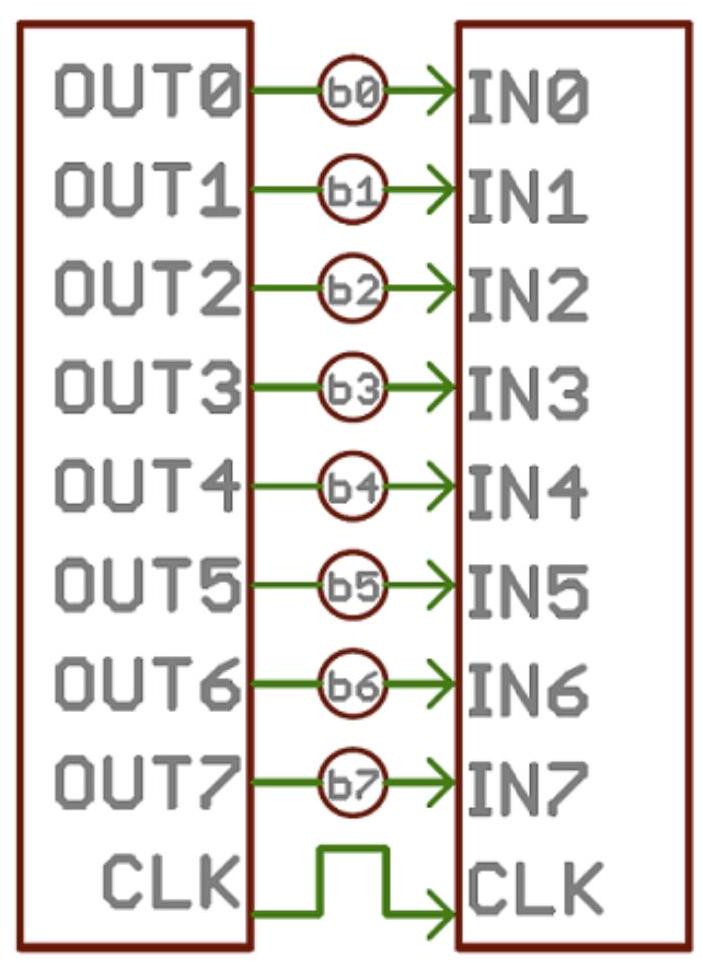
\includegraphics[max width=\textwidth]{2023_01_13_b07e3b4bcffdaab9792bg-209}
\end{center}

\begin{center}
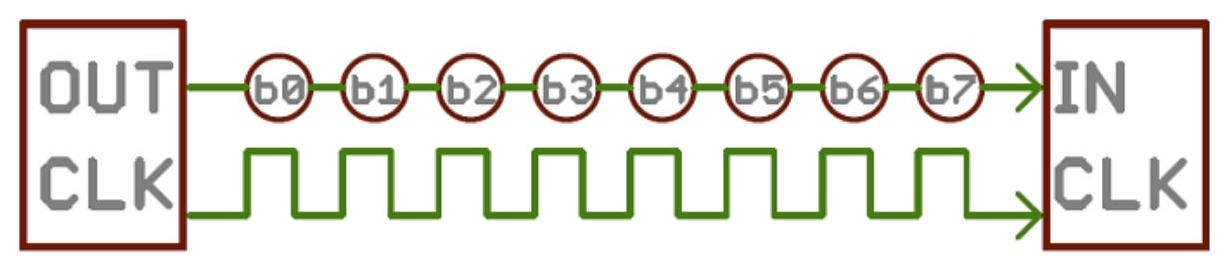
\includegraphics[max width=\textwidth]{2023_01_13_b07e3b4bcffdaab9792bg-209(1)}
\end{center}

\section{Simplistic View of Serial Port Operation Transmitter 
 Receiver}
\begin{center}
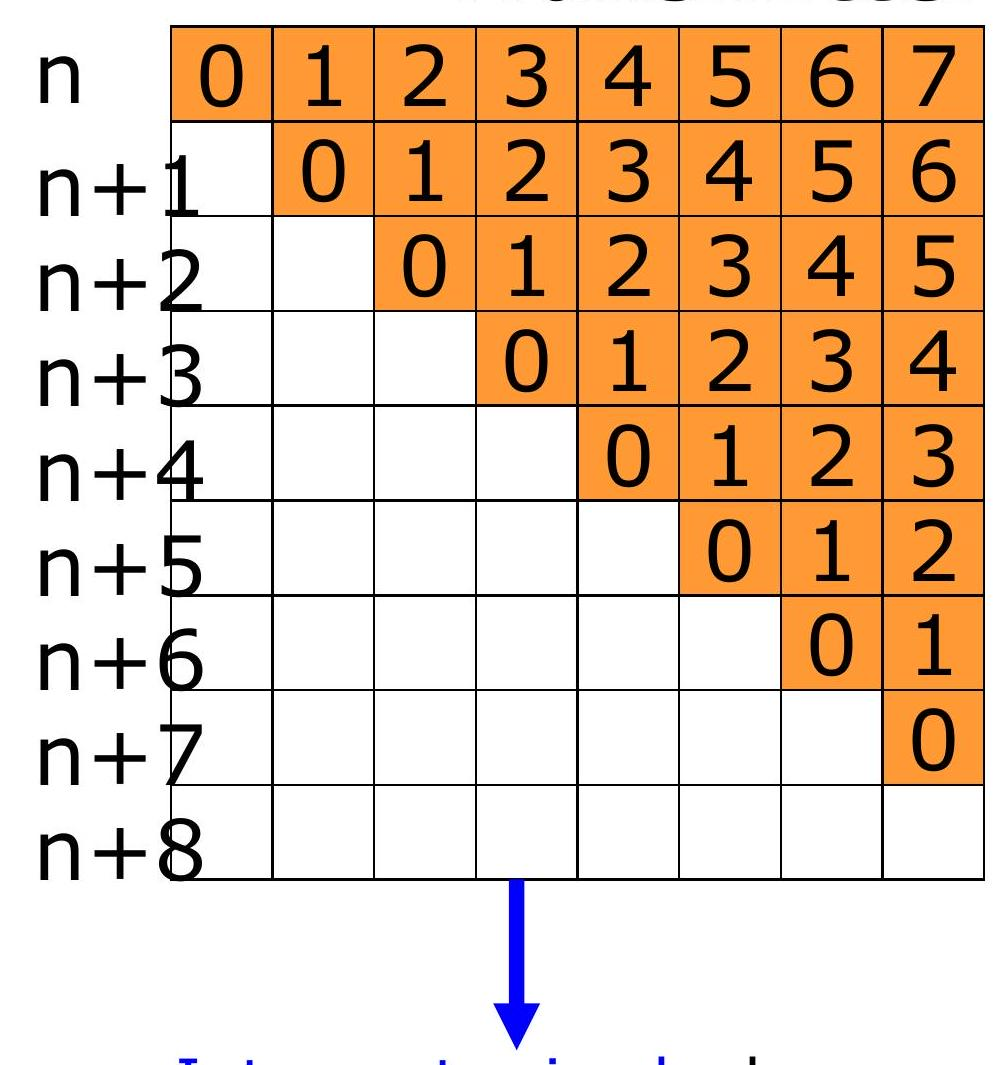
\includegraphics[max width=\textwidth]{2023_01_13_b07e3b4bcffdaab9792bg-210}
\end{center}

Interrupt raised when Transmitter $(T x)$ is empty $\Rightarrow$ Byte has been transmitted and next byte ready for loading

\begin{center}
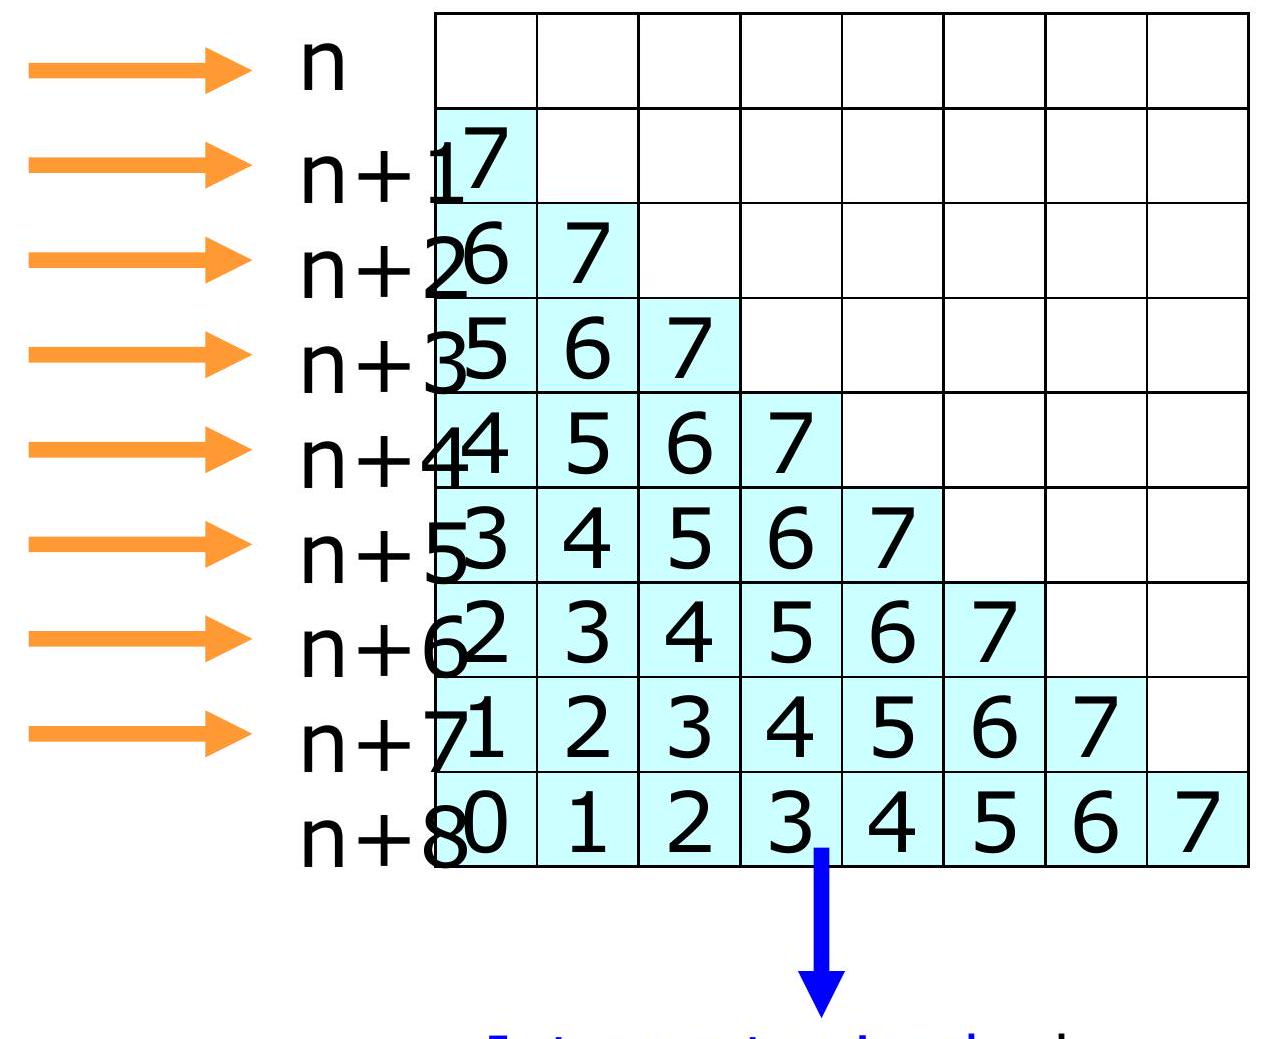
\includegraphics[max width=\textwidth]{2023_01_13_b07e3b4bcffdaab9792bg-210(1)}
\end{center}

Interrupt raised when Receiver $(R x)$ is full $\Rightarrow$ Byte has been received and is ready for reading

\section{Serial Bus Interface Motivations}
\begin{itemize}
  \item Motivation
\end{itemize}

o Without using a lot of I/O lines

$\times \mathrm{I} / \mathrm{O}$ lines require $\mathrm{I} / \mathrm{O}$ pads which cost $\$ \$ \$$ and size

\begin{itemize}
  \item I/O lines require PCB area which costs $\$ \$ \$$ and size
\end{itemize}

o Connect different systems together

\begin{itemize}
  \item Two embedded systems
\end{itemize}

$\times$ A desktop and an embedded system

o Connect different chips together in the same embedded system

\begin{itemize}
  \item MCU to peripheral
\end{itemize}

$\times \mathrm{MCU}$ to $\mathrm{MCU}$

o Often at relatively low data rates

\begin{itemize}
  \item But sometimes at higher data rates

  \item So, what are our options?

\end{itemize}

o Universal Synchronous/Asynchronous Receiver Transmitter

\begin{itemize}
  \item Also known as USART (pronounced: "you-sart")
\end{itemize}

\section{Serial Bus Design Space}
\begin{itemize}
  \item Number of wires required?

  \item Asynchronous or synchronous?

  \item How fast can it transfer data?

  \item Can it support more than two endpoints?

  \item Can it support more than one master (i.e. txn initiator)?

  \item How do we support flow control?

  \item How does it handle errors/noise?

  \item How far can signals travel?

\end{itemize}

\section{Serial Bus Examples}
\begin{center}
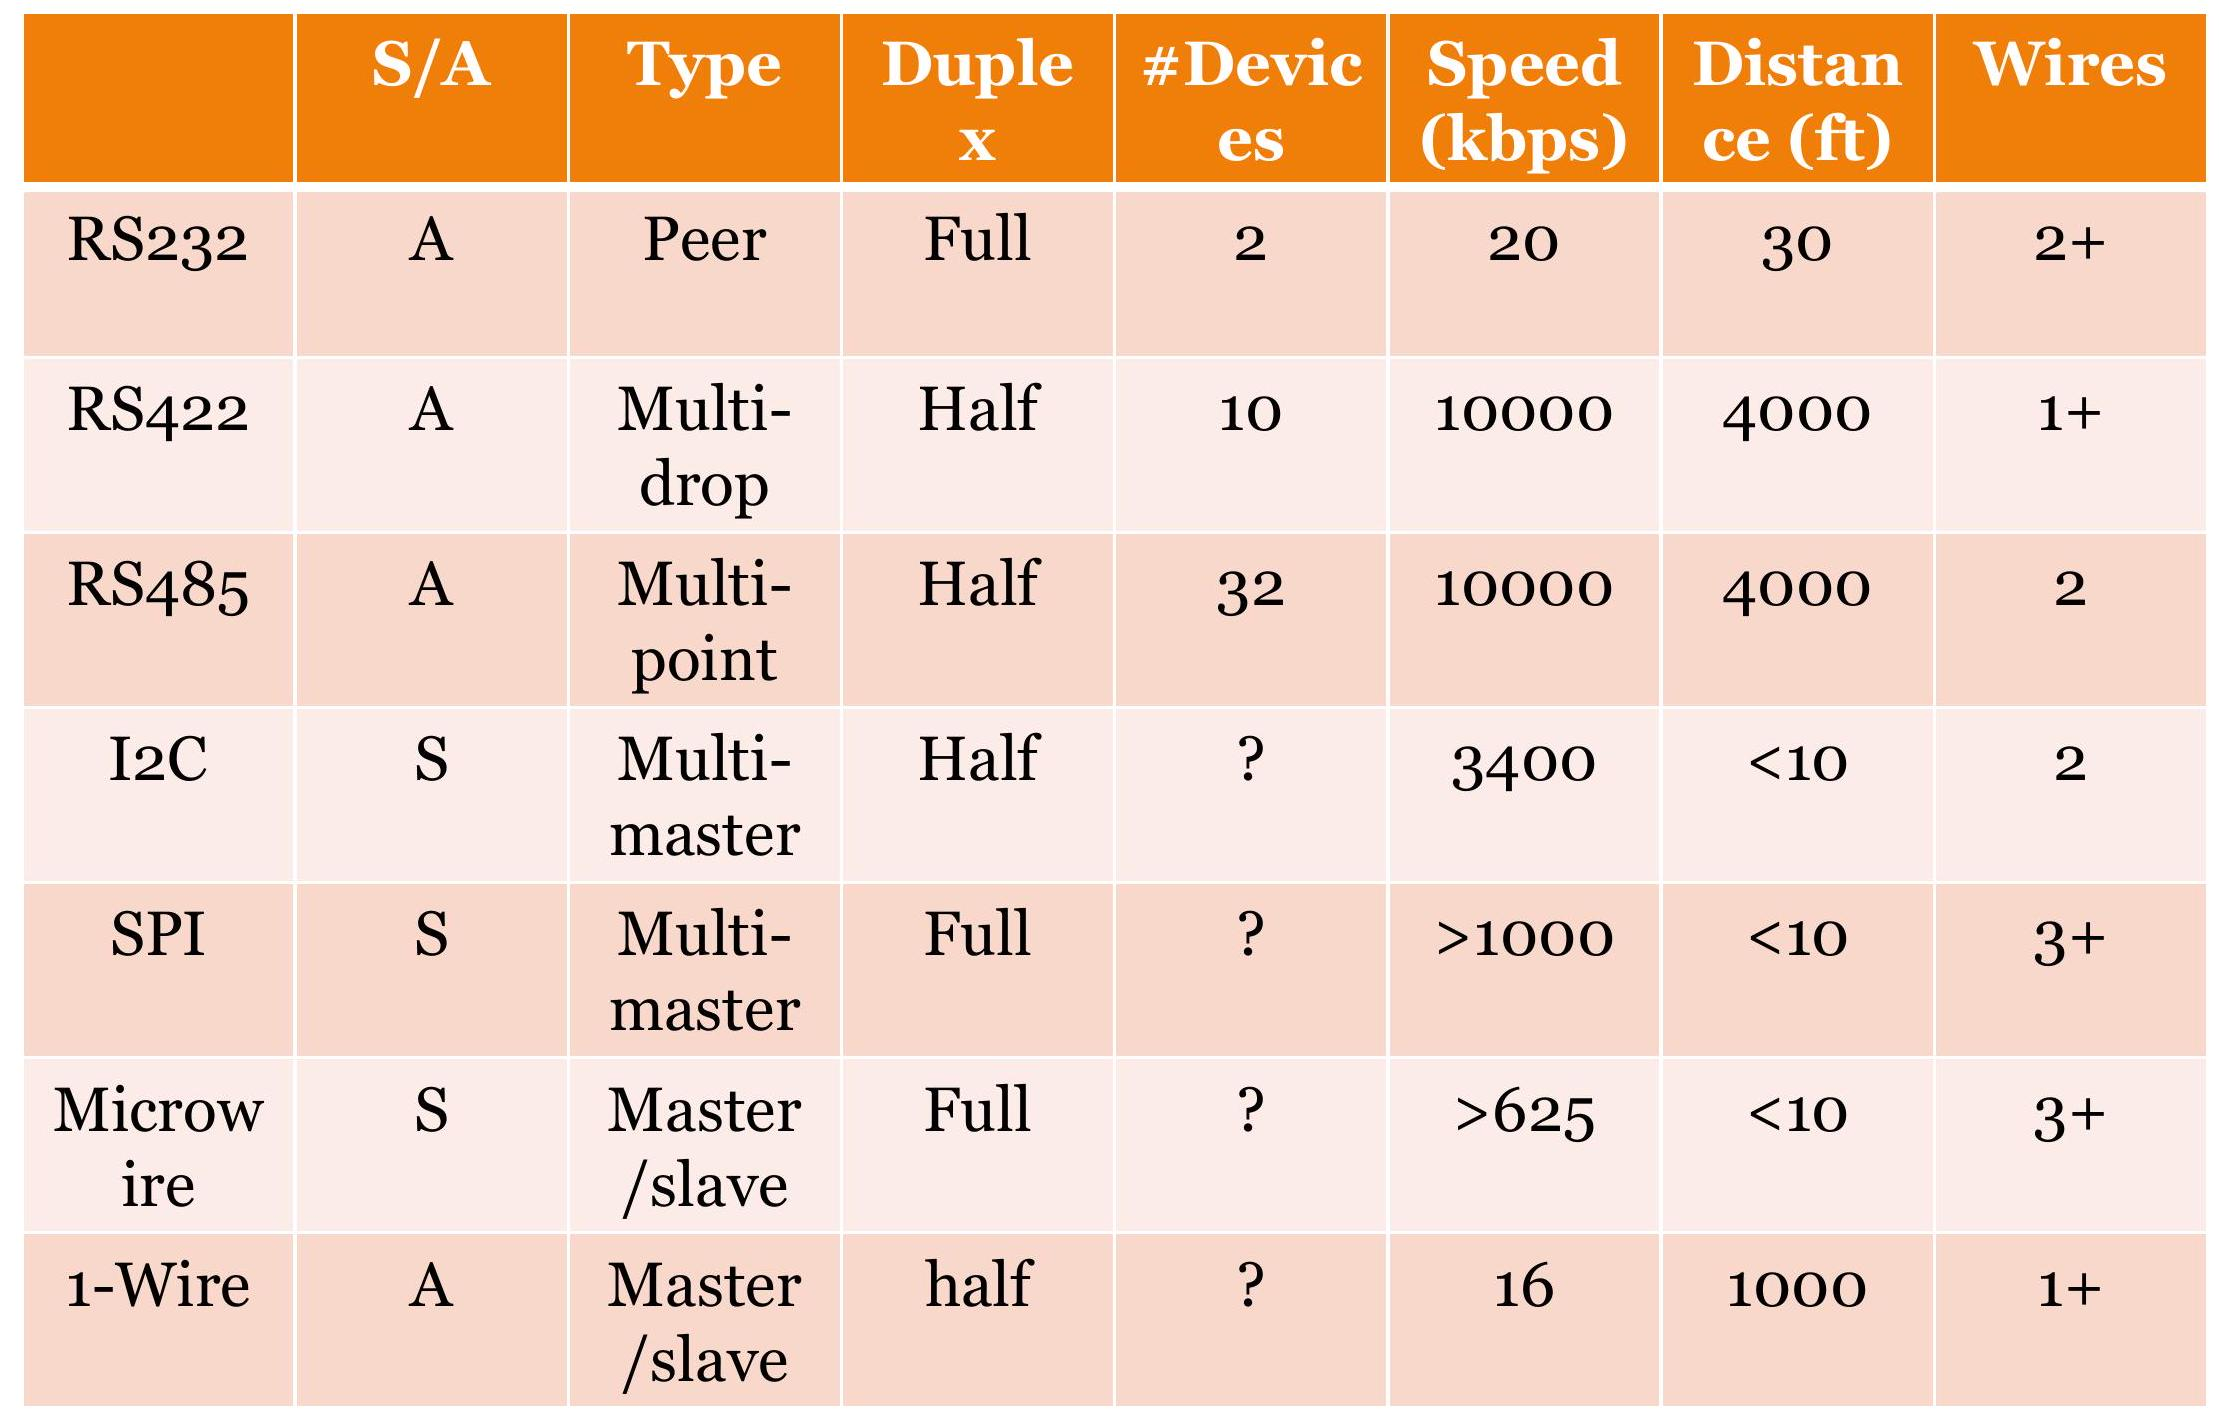
\includegraphics[max width=\textwidth]{2023_01_13_b07e3b4bcffdaab9792bg-213}
\end{center}

\section{UART Uses}
\begin{itemize}
  \item PC serial port is a UART!

  \item Serializes data to be sent over serial cable - De-serializes received data
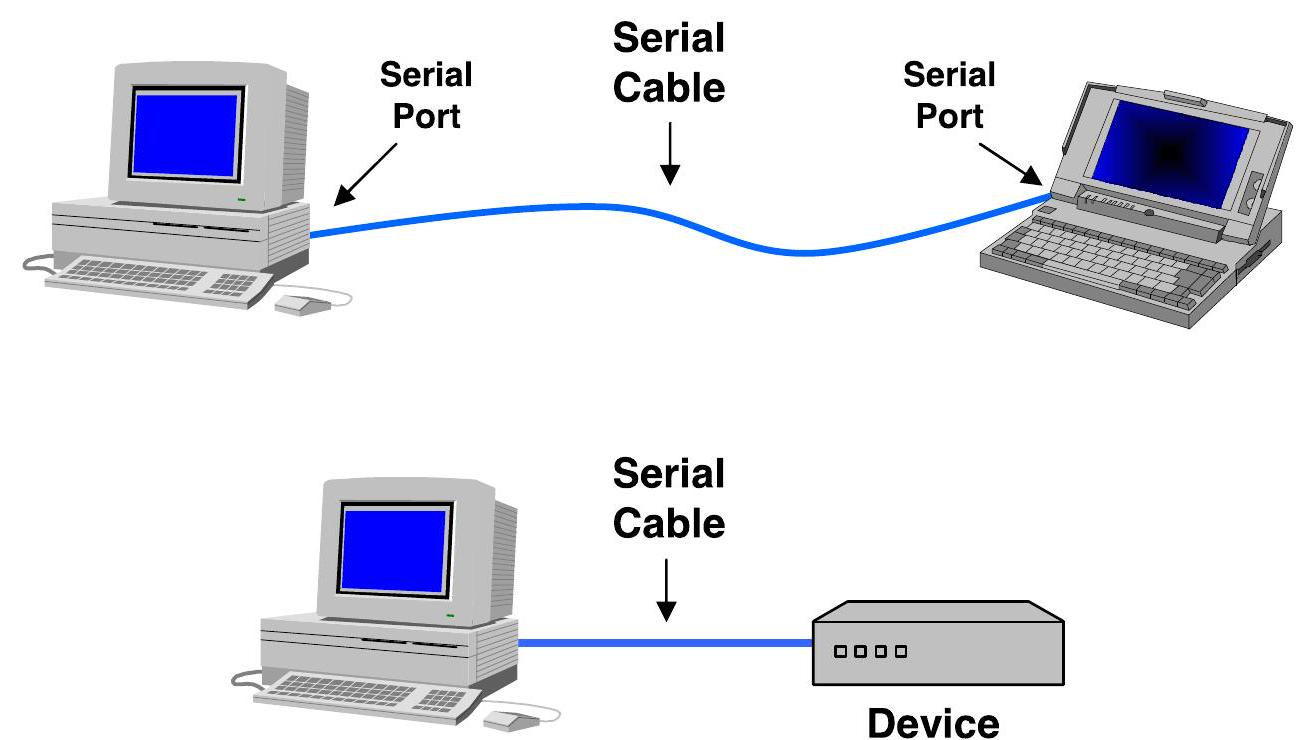
\includegraphics[max width=\textwidth, center]{2023_01_13_b07e3b4bcffdaab9792bg-214}

\end{itemize}

\section{UART Uses}
\section{- Used to be commonly used for internet access}
\begin{center}
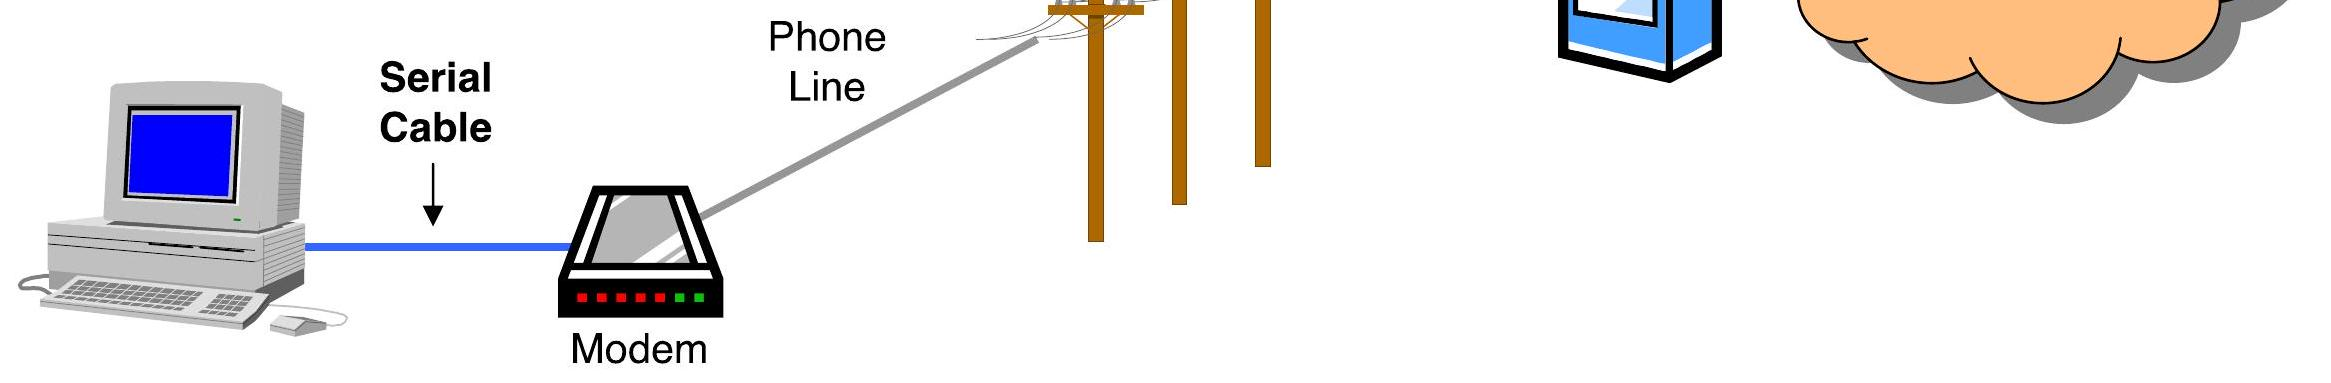
\includegraphics[max width=\textwidth]{2023_01_13_b07e3b4bcffdaab9792bg-215}
\end{center}

\section{UART}
\begin{itemize}
  \item Universal Asynchronous Receiver/Transmitter

  \item Hardware that translates between parallel and serial forms

\end{itemize}

\section{- Commonly used in conjunction with communication standards such as EIA, RS-232, RS-422 or RS-485}
\begin{center}
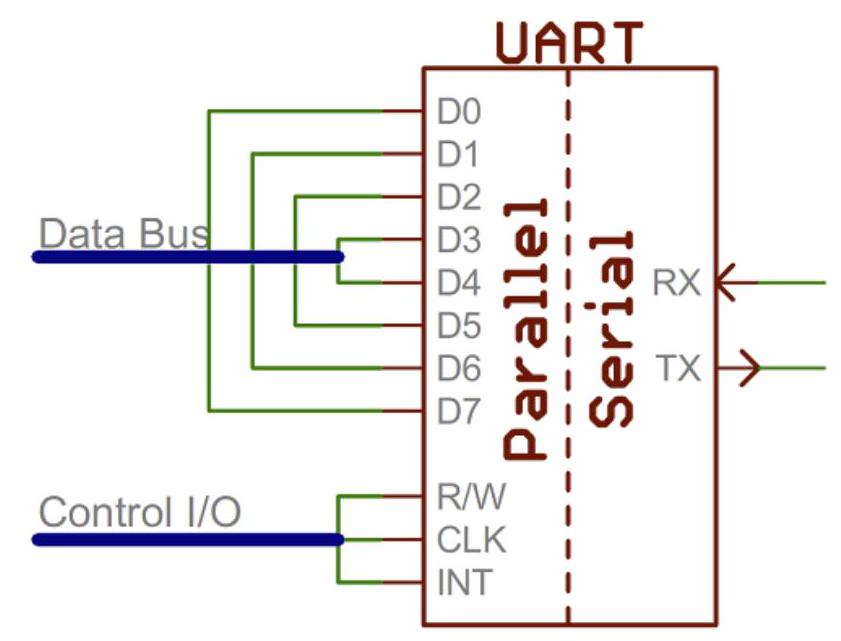
\includegraphics[max width=\textwidth]{2023_01_13_b07e3b4bcffdaab9792bg-216}
\end{center}

\section{Protocol}
\begin{itemize}
  \item Each character is sent as
\end{itemize}

o a logic low start bit

o a configurable number of data bits (usually 7 or 8 , sometimes

5.

o an optional parity bit

o one or more logic high stop bits

o with a particular bit timing ("baud")

\begin{center}
\begin{tabular}{|c|c|c|c|c|c|c|c|c|c|}
\hline
Start & Data 0 & Data 1 & Data 2 & Data 3 & Data & Data & Data & Data \\
5 & 6 & 7 & Stop &  &  &  &  &  \\
\hline
\end{tabular}
\end{center}

\section{UART Example}
\section{- Send the ASCII letter 'W' (1010111)}
\begin{center}
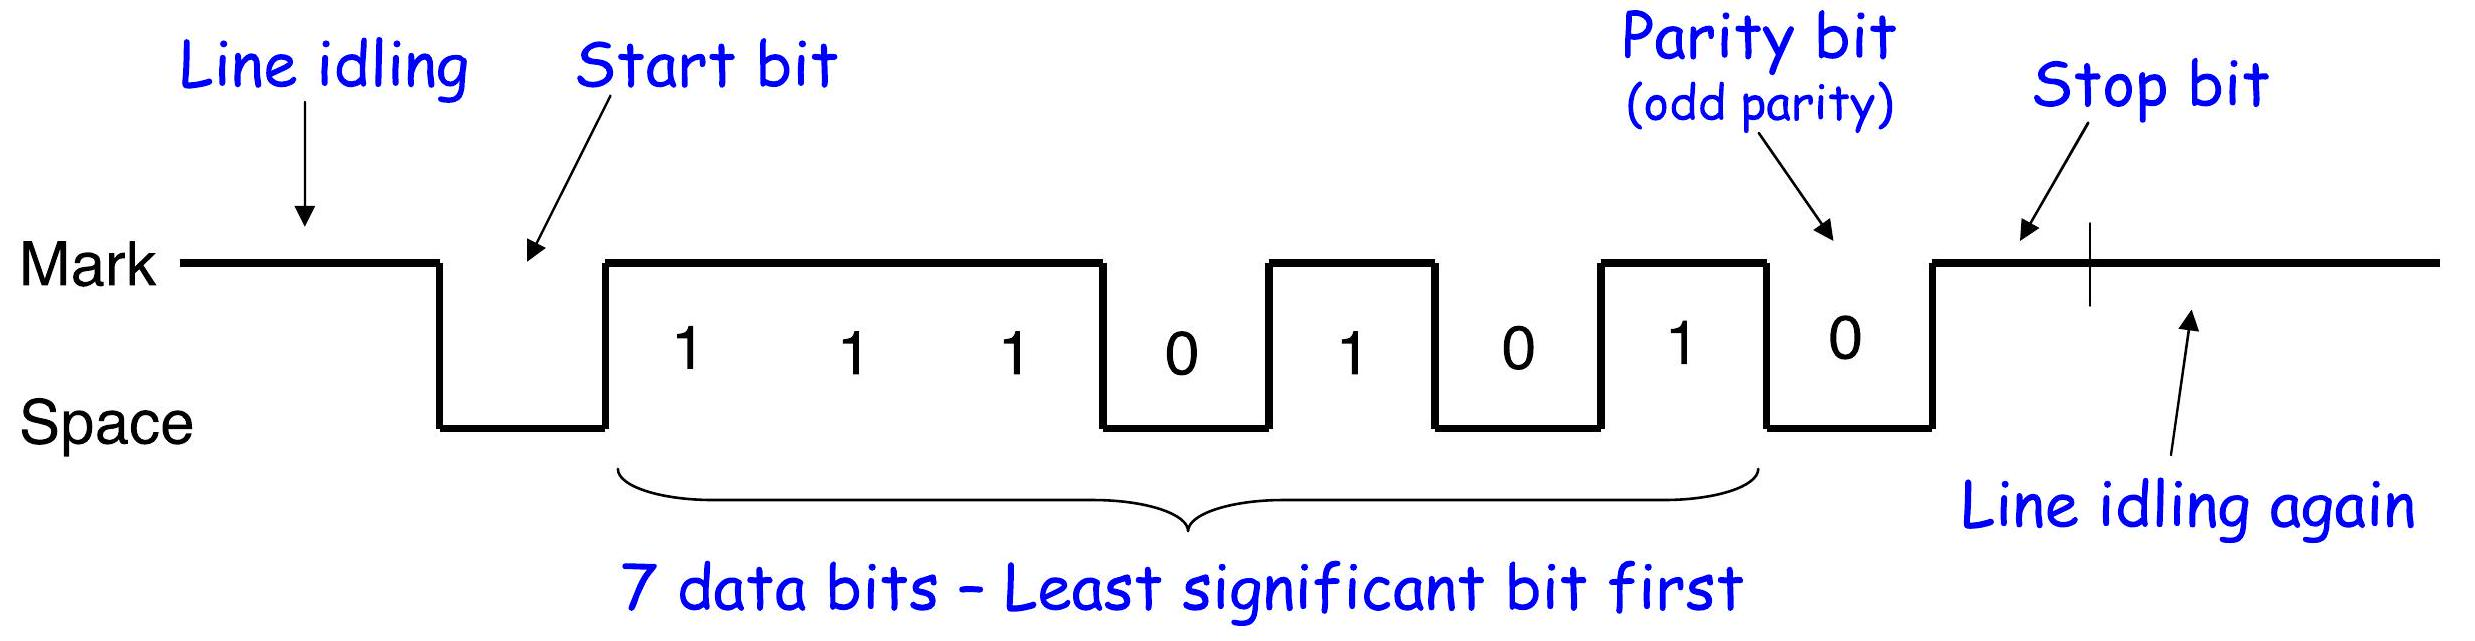
\includegraphics[max width=\textwidth]{2023_01_13_b07e3b4bcffdaab9792bg-218}
\end{center}

\section{UART Hardware Connection}
\begin{center}
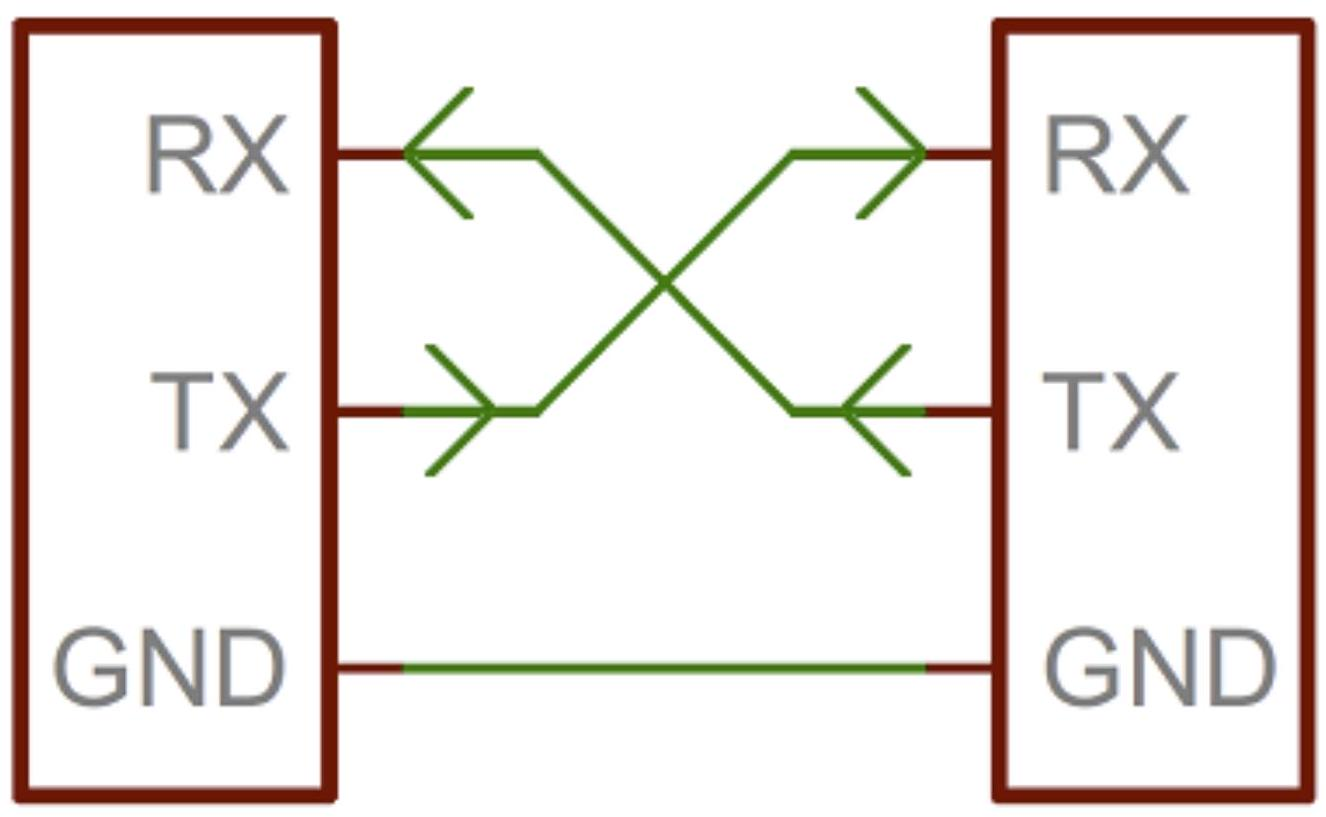
\includegraphics[max width=\textwidth]{2023_01_13_b07e3b4bcffdaab9792bg-219}
\end{center}

\section{UART Character Reception}
Start bit says a character is coming, receiver resets its timers

\begin{center}
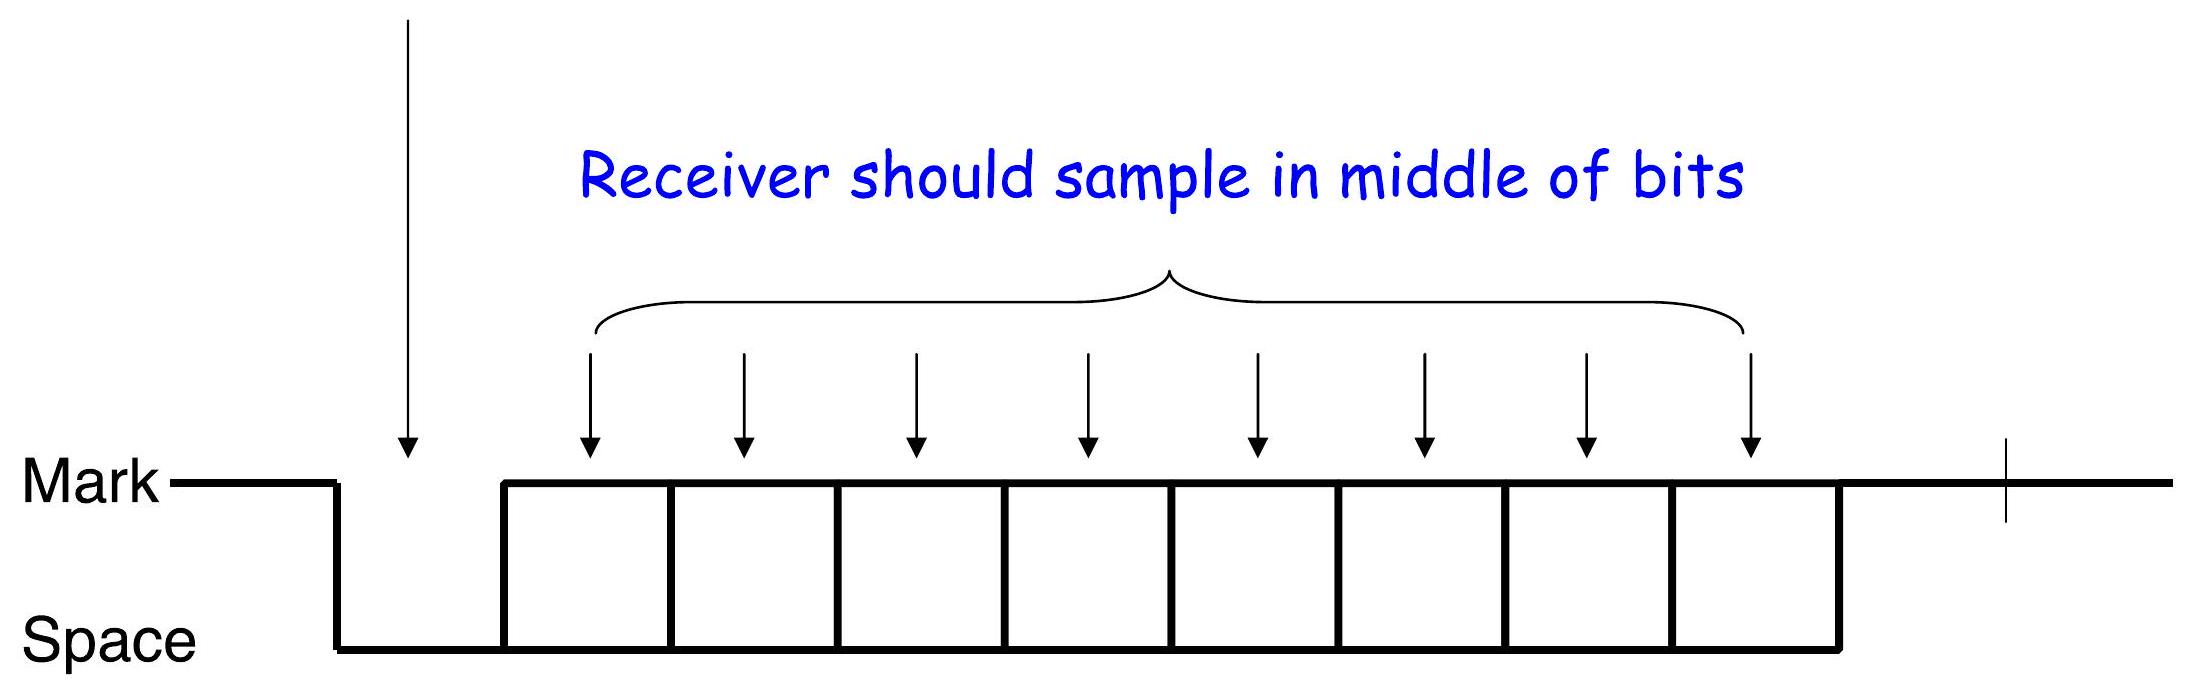
\includegraphics[max width=\textwidth]{2023_01_13_b07e3b4bcffdaab9792bg-220}
\end{center}

Receiver uses a timer (counter) to time when it samples.

Transmission rate (i.e., bit width) must be known!

Slides from BYU CS 224

\section{UART Character Reception}
If receiver samples too quickly, see what happens...

Space

\begin{center}
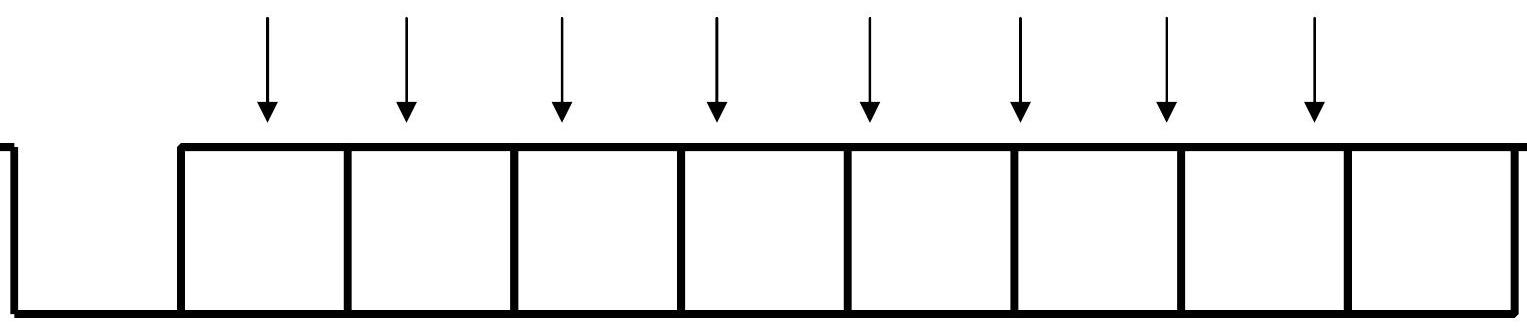
\includegraphics[max width=\textwidth]{2023_01_13_b07e3b4bcffdaab9792bg-221}
\end{center}

\section{UART Character Reception}
If receiver samples too slowly, see what happens...

Mark

Space

\begin{center}
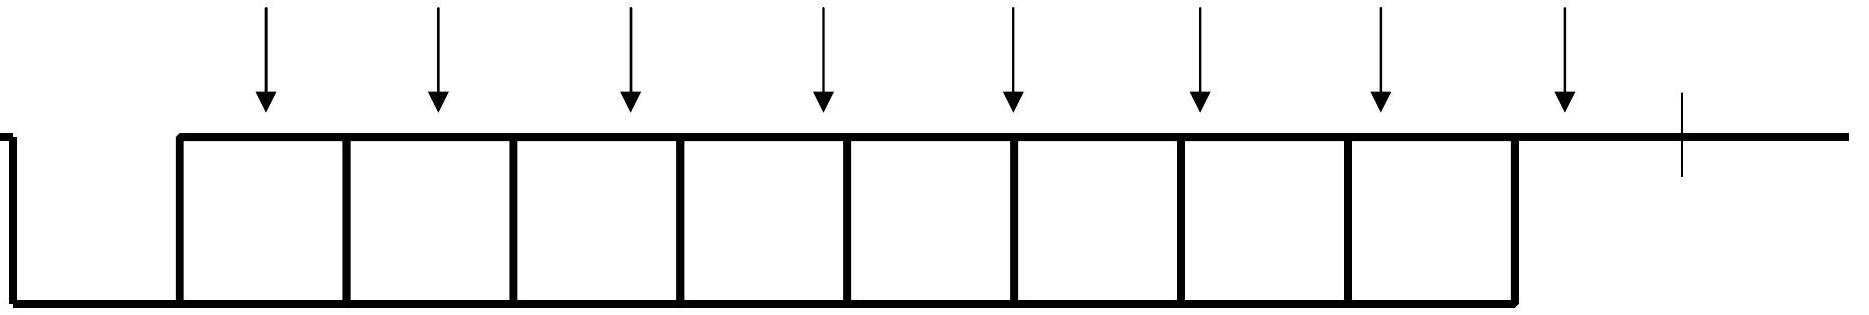
\includegraphics[max width=\textwidth]{2023_01_13_b07e3b4bcffdaab9792bg-222}
\end{center}

Receiver resynchronizes on every start bit. Only has to be accurate enough to read 9 bits.

\section{UART Character Reception}
\begin{itemize}
  \item Receiver also verifies that stop bit is ' 1 '

  \item If not, reports "framing error" to host system

  \item New start bit can appear immediately after stop bit - Receiver will resynchronize on each start bit

\end{itemize}

\section{Let us design a UART transmitter}
\begin{center}
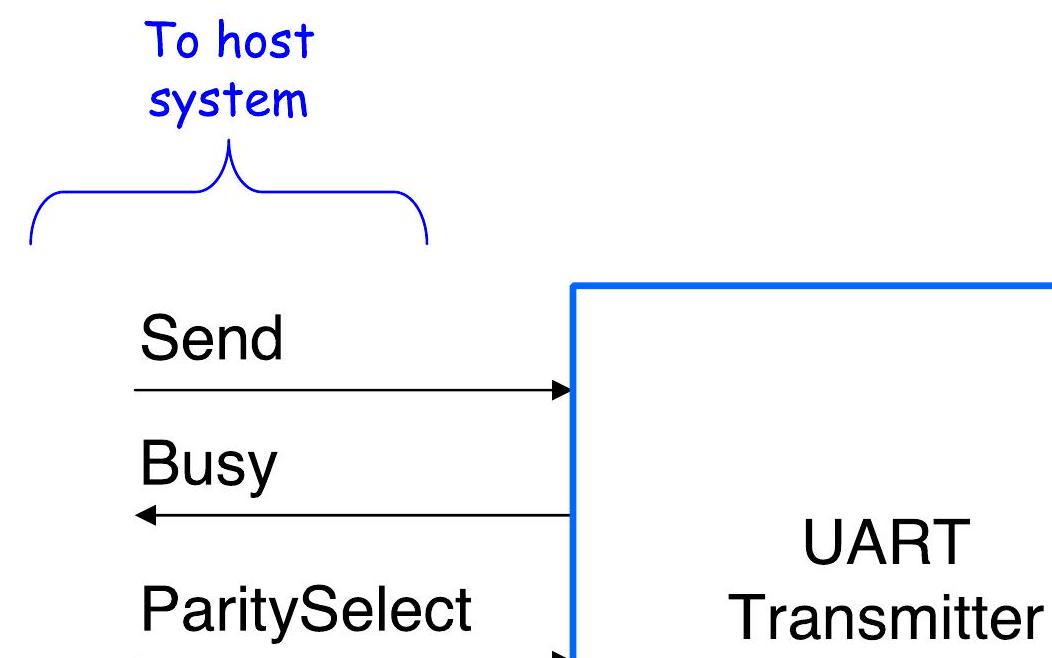
\includegraphics[max width=\textwidth]{2023_01_13_b07e3b4bcffdaab9792bg-224}
\end{center}

\section{Transmitter/System Handshaking}
\begin{itemize}
  \item System asserts Send and holds it high when it wants to send a byte

  \item UART asserts Busy signal in response

  \item When UART has finished transfer, UART de-asserts Busy signal

  \item System de-asserts Send signal
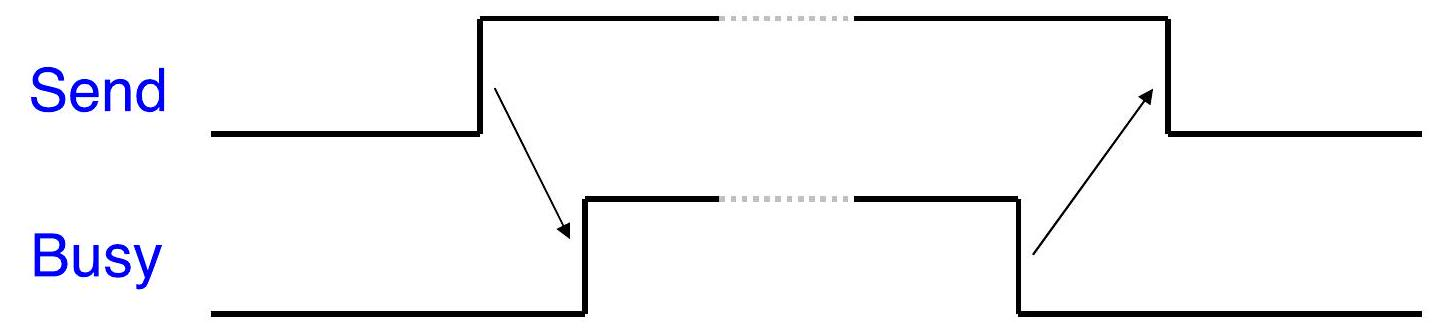
\includegraphics[max width=\textwidth, center]{2023_01_13_b07e3b4bcffdaab9792bg-225}

\end{itemize}

\section{Transmitter Block Diagram}
\begin{center}
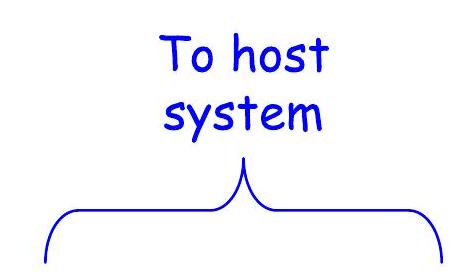
\includegraphics[max width=\textwidth]{2023_01_13_b07e3b4bcffdaab9792bg-226}
\end{center}

Send

\begin{center}
\begin{tabular}{l}
Busy \\
\hline
ParitySelect \\
\hline
\end{tabular}
\end{center}

ParitySelect

Din $300 \mathrm{HZ}$

Timer

Mod10

Counter State

Machine

Parity

Generator Shift

Register

\section{Discussion Questions}
\begin{itemize}
  \item How fast can we run a UART?

  \item What are the limitations?

  \item Why do we need start/stop bits?

  \item How many data bits can be sent?

\end{itemize}

19200 baud rate, no parity, 8 data bits, 1 stop bit

\section{Serial Peripheral Interconnect (SPI)}
\begin{itemize}
  \item Another kind of serial protocol in embedded systems (proposed by Motorola)

  \item Four-wire protocol o SCLK - Serial Clock

  \item MOSI/SIMO - Master Output, Slave Input

  \item MISO/SOMI - Master Input, Slave Output

  \item SS - Slave Select

  \item Single master device and with one or more slave devices

  \item Higher throughput than I2C and can do "stream transfers"

  \item No arbitration required

  \item But

  \item Requires more pins

  \item Has no hardware flow control

  \item No slave acknowledgment (master could be talking to thin air and not even know it)

\end{itemize}

\section{What is SPI?}
\begin{itemize}
  \item Serial Bus protocol

  \item Fast, \href{http://Easy.to}{Easy.to} use, Simpleat ..... ° - Everyor'

\end{itemize}

\begin{center}
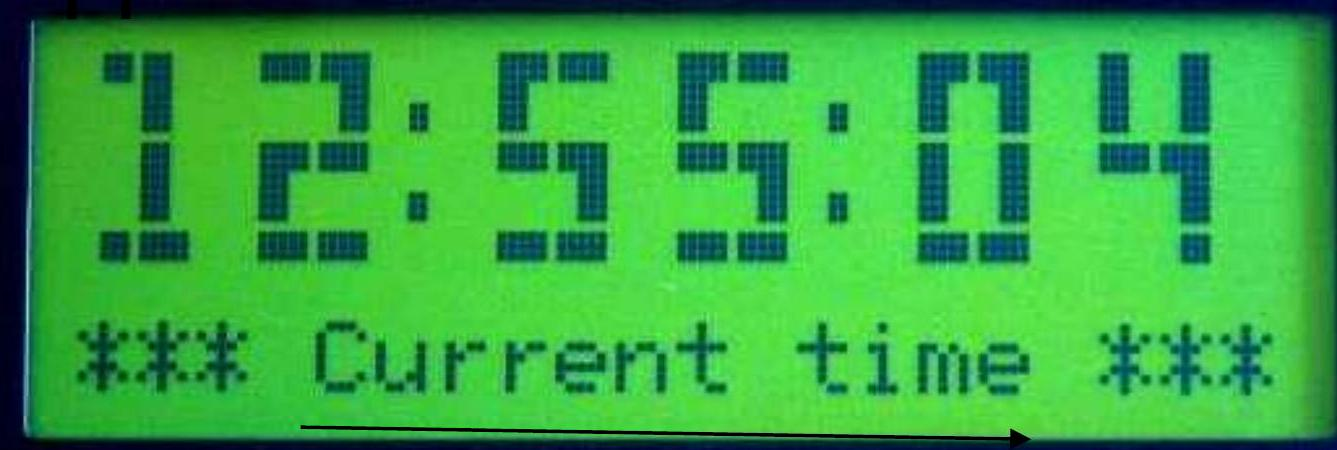
\includegraphics[max width=\textwidth]{2023_01_13_b07e3b4bcffdaab9792bg-229}
\end{center}

\begin{center}
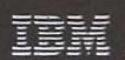
\includegraphics[max width=\textwidth]{2023_01_13_b07e3b4bcffdaab9792bg-229(1)}
\end{center}

Digital Set-Top Box Integrated Controller

POWCNDET

75H6051 03BM 1F11DOORPB KOREA

\begin{center}
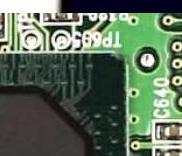
\includegraphics[max width=\textwidth]{2023_01_13_b07e3b4bcffdaab9792bg-229(2)}
\end{center}

IBM39 STB02100 PBC 22C



\section{SPI Basics}
\section{- A communication protocol using 4 wires Also known as a 4 wire bus}
\section{- Used to communicate across small distances}
\section{- Multiple Slaves, Single Master}
\section{- Synchronized}
\section{SPI Capabilities}
\begin{itemize}
  \item Always Full Duplex

  \item Communicating in two directions at the same time

  \item Transmission need not be meaningful

  \item Multiple Mbps transmission speed

\end{itemize}

\section{- Transfers data in 4 to 16 bit characters}
\begin{itemize}
  \item Multiple slaves

  \item Daisy-chaining possible

\end{itemize}

\section{SPI Protocol}
\begin{itemize}
  \item Wires:
\end{itemize}

o Master Out Slave In (MOSI)

o Master In Slave Out (MISO)

o System Clock (SCLK)

\begin{itemize}
  \item Slave Select 1...N
\end{itemize}

\begin{center}
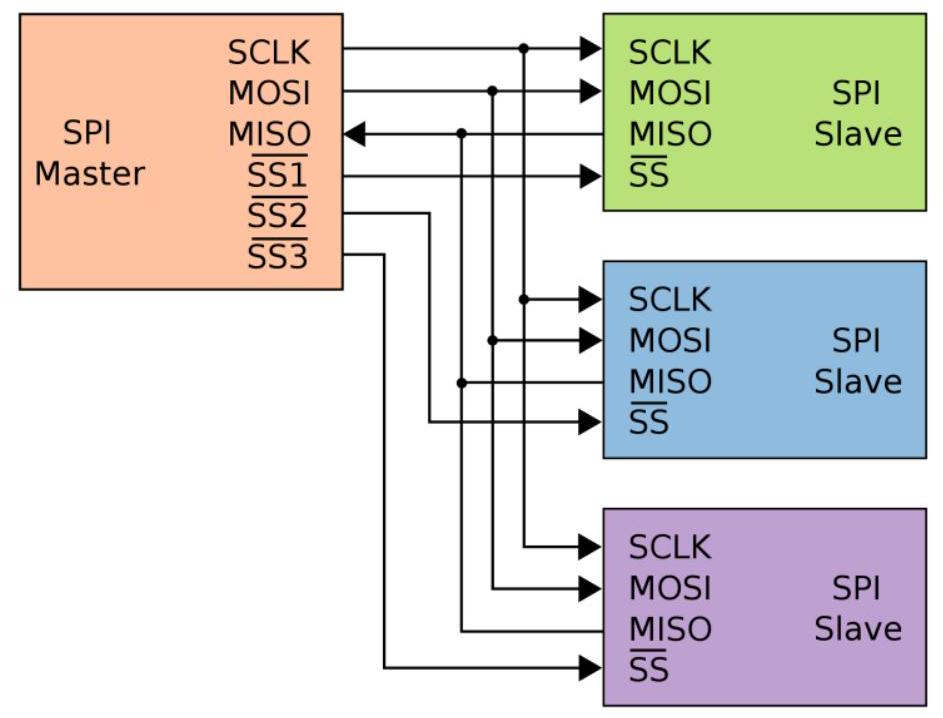
\includegraphics[max width=\textwidth]{2023_01_13_b07e3b4bcffdaab9792bg-232}
\end{center}

\begin{itemize}
  \item Master Generates Clock

  \item Master Set Slave Select low

  \item Shift registers shift in and out data

\end{itemize}

\section{SPI Wires in Detail}
\section{- MOSI - Carries data out of Master to Slave}
\begin{itemize}
  \item MISO - Carries data from Slave to Master - Both signals happen for every transmission

  \item SS\_BAR - Unique line to select a slave

\end{itemize}

\section{- SCLK - Master produced clock to synchronize data transfer}
\begin{center}
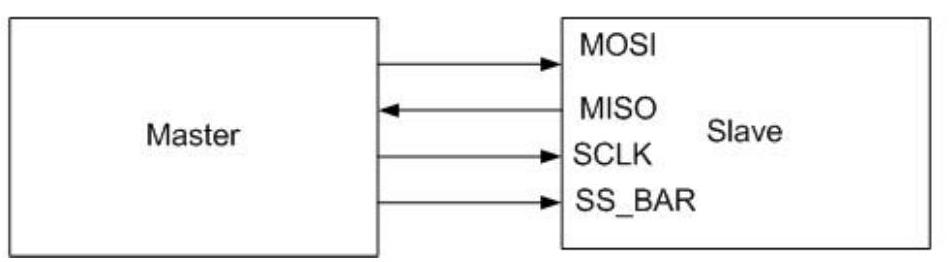
\includegraphics[max width=\textwidth]{2023_01_13_b07e3b4bcffdaab9792bg-233}
\end{center}

\section{SPI uses a "shift register" model of communications}
\section{Master}
Slave

\begin{center}
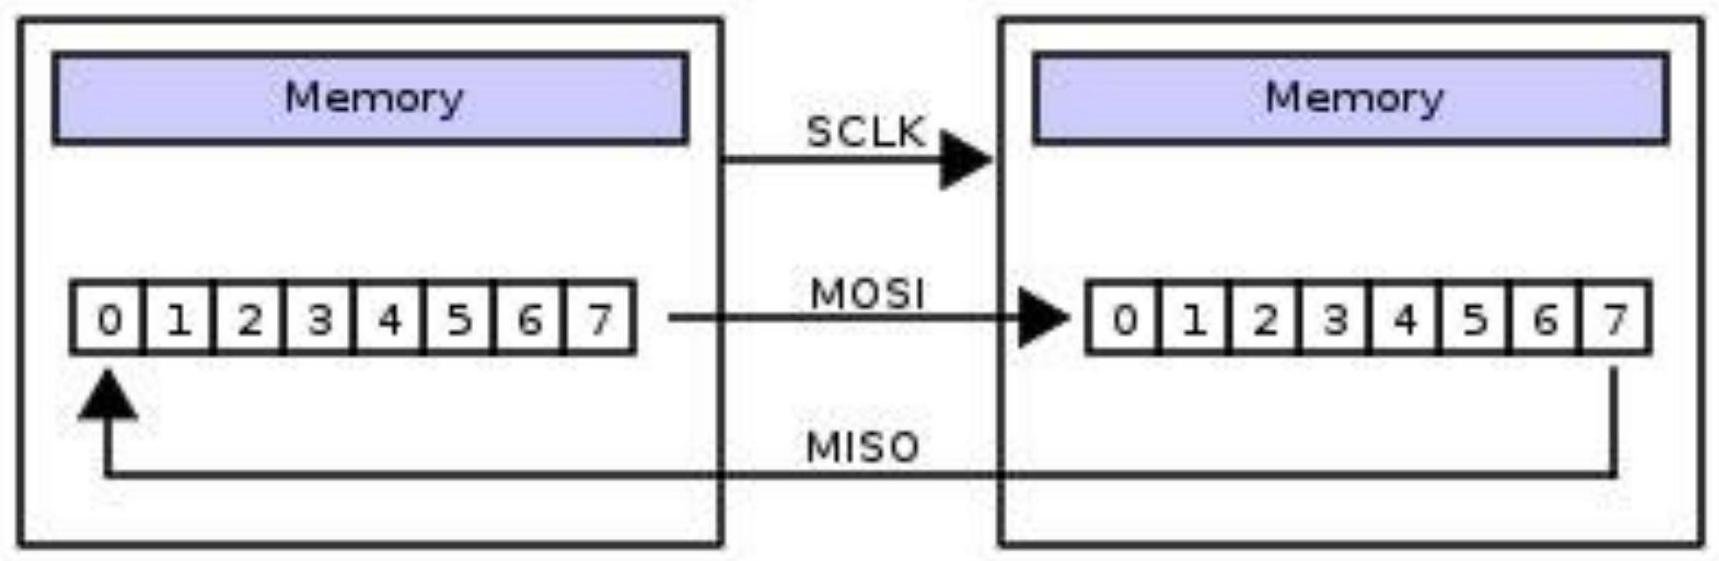
\includegraphics[max width=\textwidth]{2023_01_13_b07e3b4bcffdaab9792bg-234}
\end{center}

Master shifts out data to Slave, and shifts in data from Slave \href{http://upload.wikimedia.org/wikipedia/commons/thumb/b/bb/SPI_8-bit_circular_transfer.svg/400px-SPI_8-bit_circular_transfer.svg.png}{http://upload.wikimedia.org/wikipedia/commons/thumb/b/bb/SPI\_8-bit\_circular\_transfer.svg/400px-SPI\_8-bit\_circular\_transfer.svg.png}

\section{SPI Communication}
\begin{center}
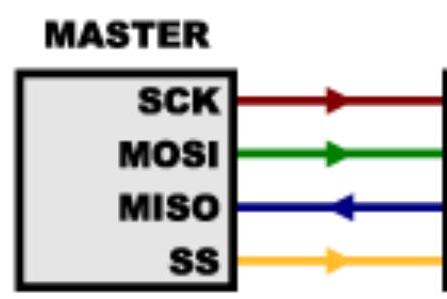
\includegraphics[max width=\textwidth]{2023_01_13_b07e3b4bcffdaab9792bg-235}
\end{center}

SLAVE

SCK

MosI

MISO

Ss

\begin{center}
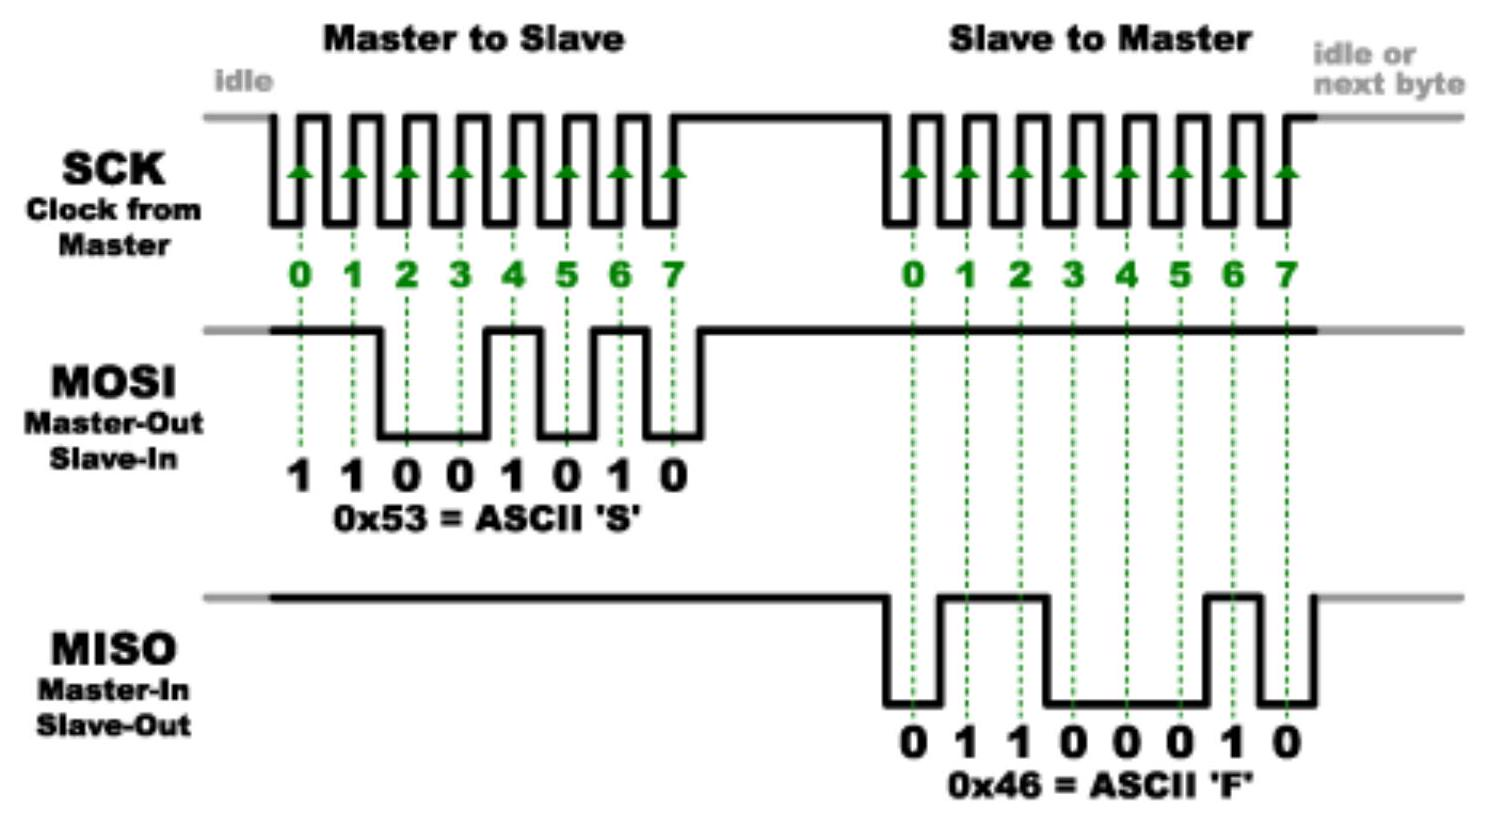
\includegraphics[max width=\textwidth]{2023_01_13_b07e3b4bcffdaab9792bg-235(1)}
\end{center}

\begin{center}
\begin{tabular}{c|l|l}
SS \\
Slave-Select \\
\end{tabular}
\end{center} 

\section{SPI clocking: there is no "standard way"}
\begin{itemize}
  \item Four clocking “modes"

  \item Two phases

  \item Two polarities

  \item Master and selected slave must be in the same mode

  \item During transfers with slaves A and B, Master must

  \item Configure clock to Slave A's clock mode

  \item Select Slave A

  \item Do transfer

  \item Deselect Slave A

  \item Configure clock to Slave B's clock mode

  \item Select Slave B

  \item Do transfer

  \item Deselect Slave B

  \item Master reconfigures clock mode on-the-fly!

\end{itemize}

\section{SPI timing diagram}
\begin{center}
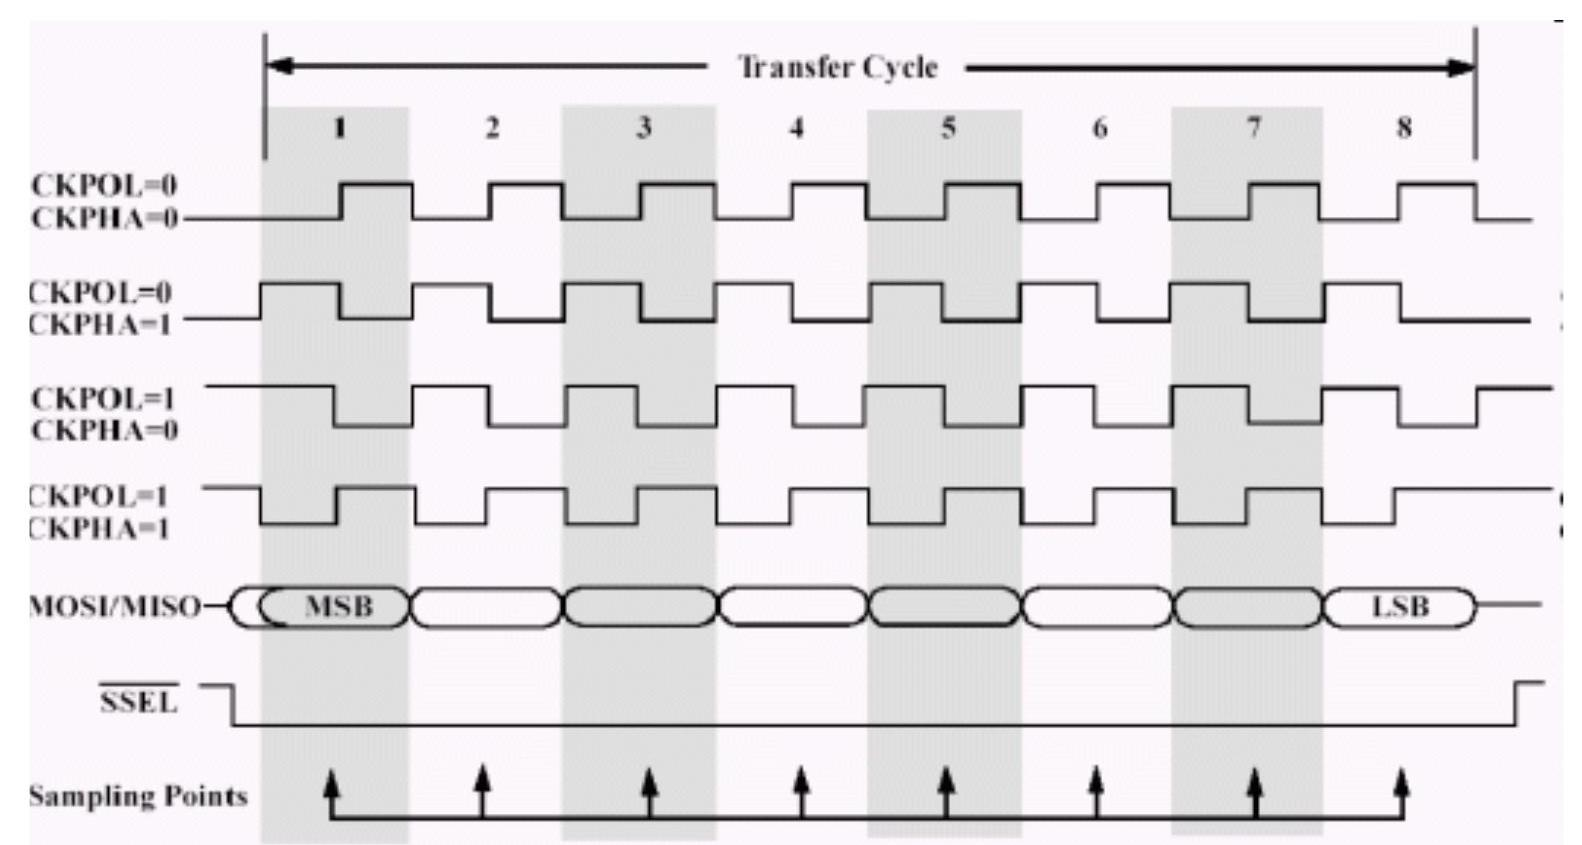
\includegraphics[max width=\textwidth]{2023_01_13_b07e3b4bcffdaab9792bg-237}
\end{center}

Timing Diagram - Showing Clock polarities and phases \href{http://www.maxim-ic.com.cn/images/appnotes/3078/3078Fig02.gif}{http://www.maxim-ic.com.cn/images/appnotes/3078/3078Fig02.gif}

\section{SPI Pros and Cons}
\begin{itemize}
  \item Pros:

  \item Fast and easy
Fast for point-to-point connections

Easily allows streaming/Constant data inflow

No addressing/Simple to implement

Everyone supports it

  \item Cons:

\end{itemize}

SS makes multiple slaves very complicated

\begin{itemize}
  \item No acknowledgement ability

  \item No inherent arbitration

\end{itemize}

No flow control

\section{I2C bus in our projects}
\begin{itemize}
  \item Communication with the accelerometer
\end{itemize}

Read from the accelerometer

\begin{itemize}
  \item Pros

  \item Simple wire connection

  \item Two wires bus that can connect multiple peripherals with the $\mathrm{MCU}$

  \item Cons

  \item Complexity is significantly higher

\end{itemize}

\section{How to operate the camera?}
Accel

\begin{center}
\begin{tabular}{|l|l|l|}
\hline
MCU \\
\hline
\end{tabular}
\end{center}

\href{https://www.youtube.com/watch?v}{https://www.youtube.com/watch?v} $=e q Z g$

xR6eRjo

\section{I2C Details}
\begin{itemize}
  \item Two lines
\end{itemize}

o Serial data line (SDA)

o Serial clock line (SCL)

\section{- Only two wires for connecting multiple devices}
\begin{center}
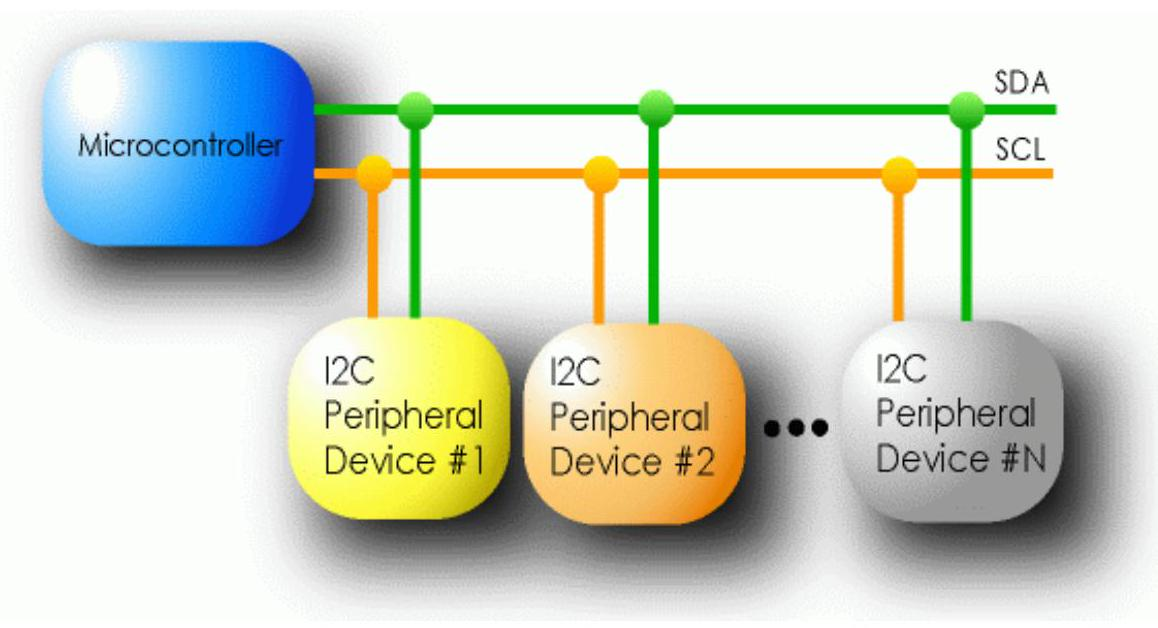
\includegraphics[max width=\textwidth]{2023_01_13_b07e3b4bcffdaab9792bg-241}
\end{center}

\section{I2C Details}
\section{- Each I2C device recognized by a unique address}
\section{- Each I2C device can be either a transmitter or receiver}
\section{- I2C devices can be masters or slaves for a data transfer}
o Master (usually a microcontroller): Initiates a data transfer on the bus, generates the clock signals to permit that transfer, and terminates the transfer

o Slave: Any device addressed by the master at that time

\section{Bit Transfer on the $\mathrm{I}^{2} \mathrm{C}$ Bus}
\begin{itemize}
  \item In normal data transfer, the data line only changes state when the clock is low
\end{itemize}

$\mathrm{SCL}$ SDA

$\mathrm{SCL}$

\begin{center}
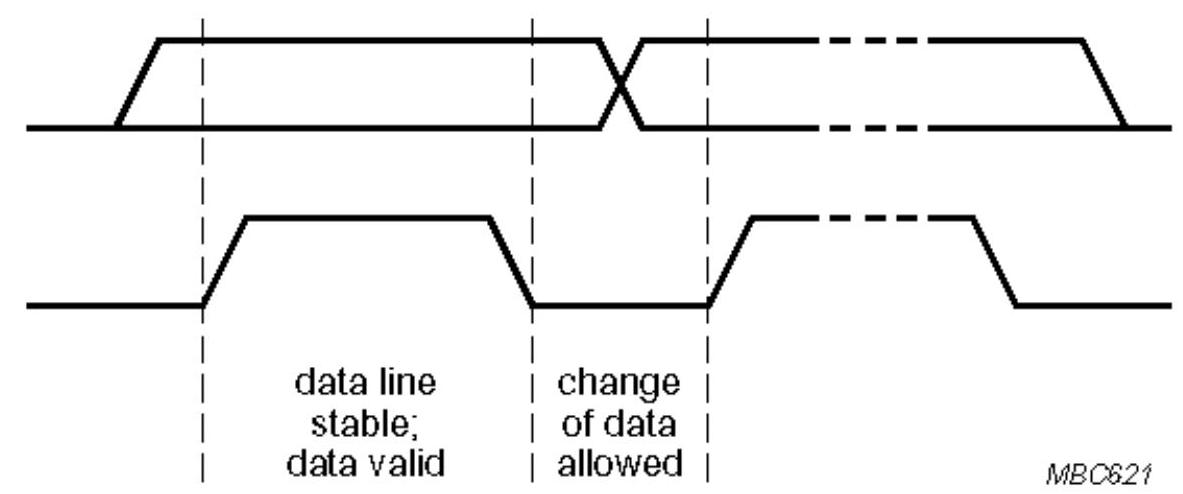
\includegraphics[max width=\textwidth]{2023_01_13_b07e3b4bcffdaab9792bg-243}
\end{center}

Data line stable; Data valid

\begin{center}
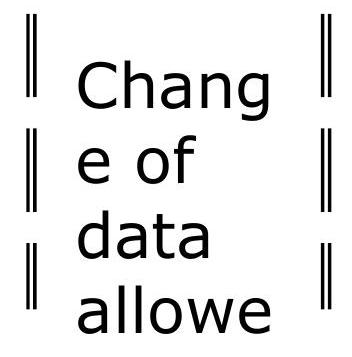
\includegraphics[max width=\textwidth]{2023_01_13_b07e3b4bcffdaab9792bg-243(1)}
\end{center}

$\mathrm{d}$

\section{Start and Stop Conditions}
A transition of the data line while the clock line is high is defined as either a start or a stop condition.

Both start and stop conditions are generated by the bus master

The bus is considered busy after a start condition, until a stop condition occurs

\begin{center}
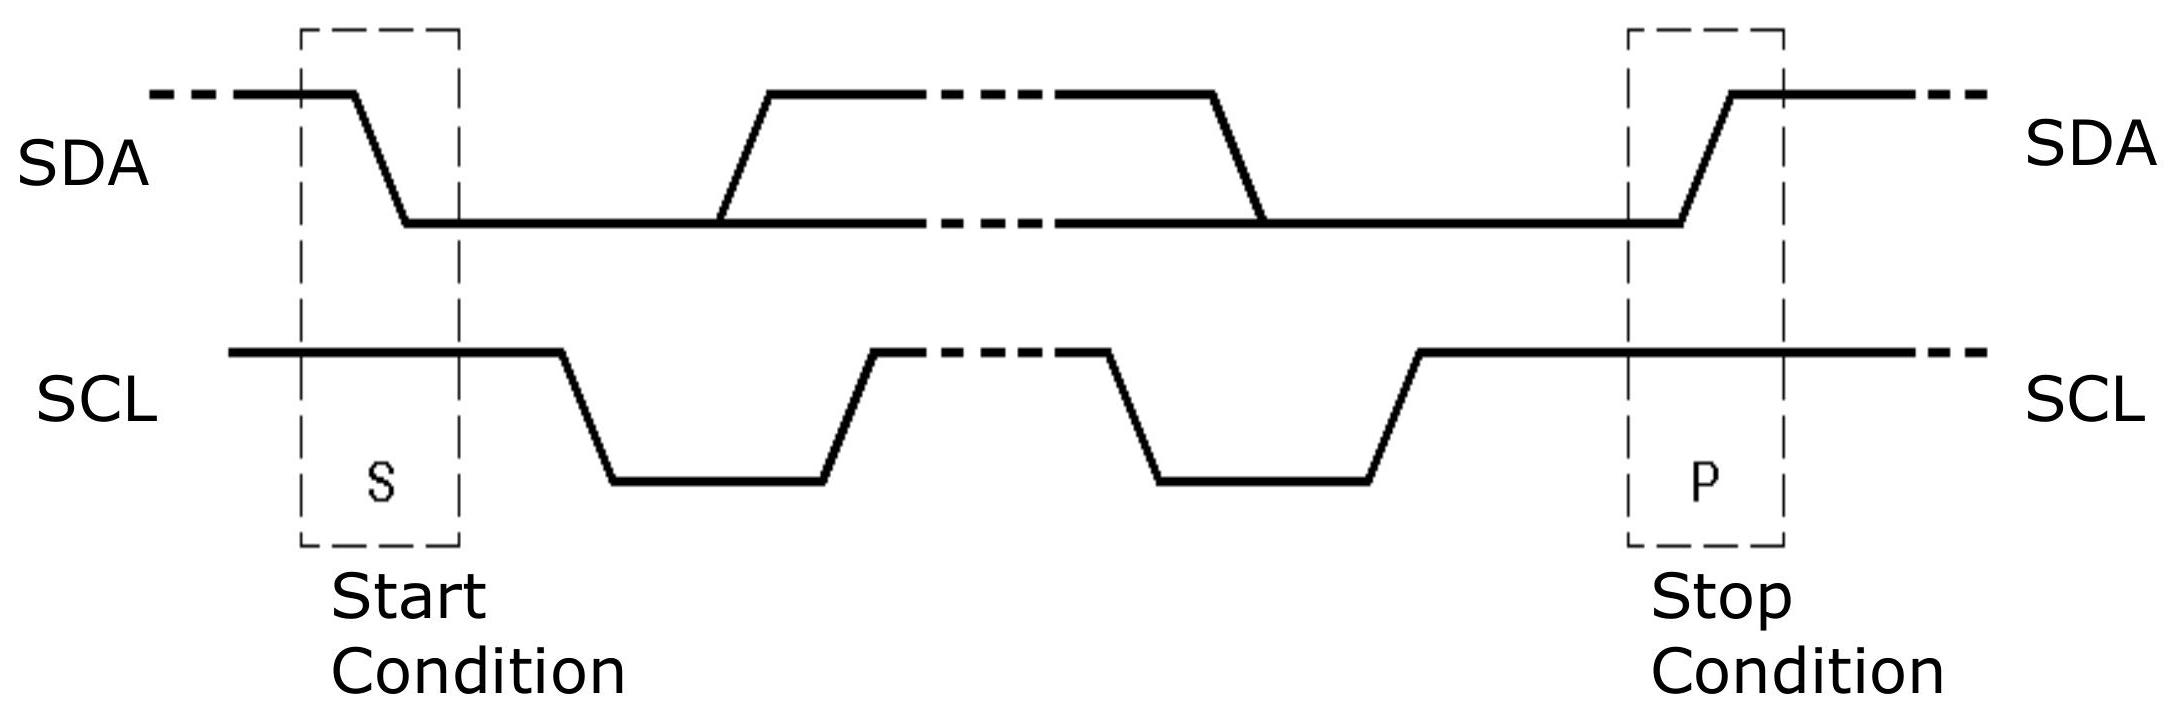
\includegraphics[max width=\textwidth]{2023_01_13_b07e3b4bcffdaab9792bg-244}
\end{center}

\section*{$\mathrm{I}^{2} \mathrm{C}$ Addressing }
\section{- Each node has a unique 7 (or 10) bit address}
\section{- Peripherals often have fixed and programmable address portions}
\section{- Addresses starting with o000 or 1111 have special functions:-}

\begin{itemize}
  \item 0000000 Is a General Call Address \textbackslash  o o000001 Is a Null (CBUS) Address \textbackslash  o 1111XXX Address Extension \textbackslash  O 1111111 Address Extension - Next Bytes are the Actual Address
\end{itemize}

\section{I2C-Connected System}
\begin{center}
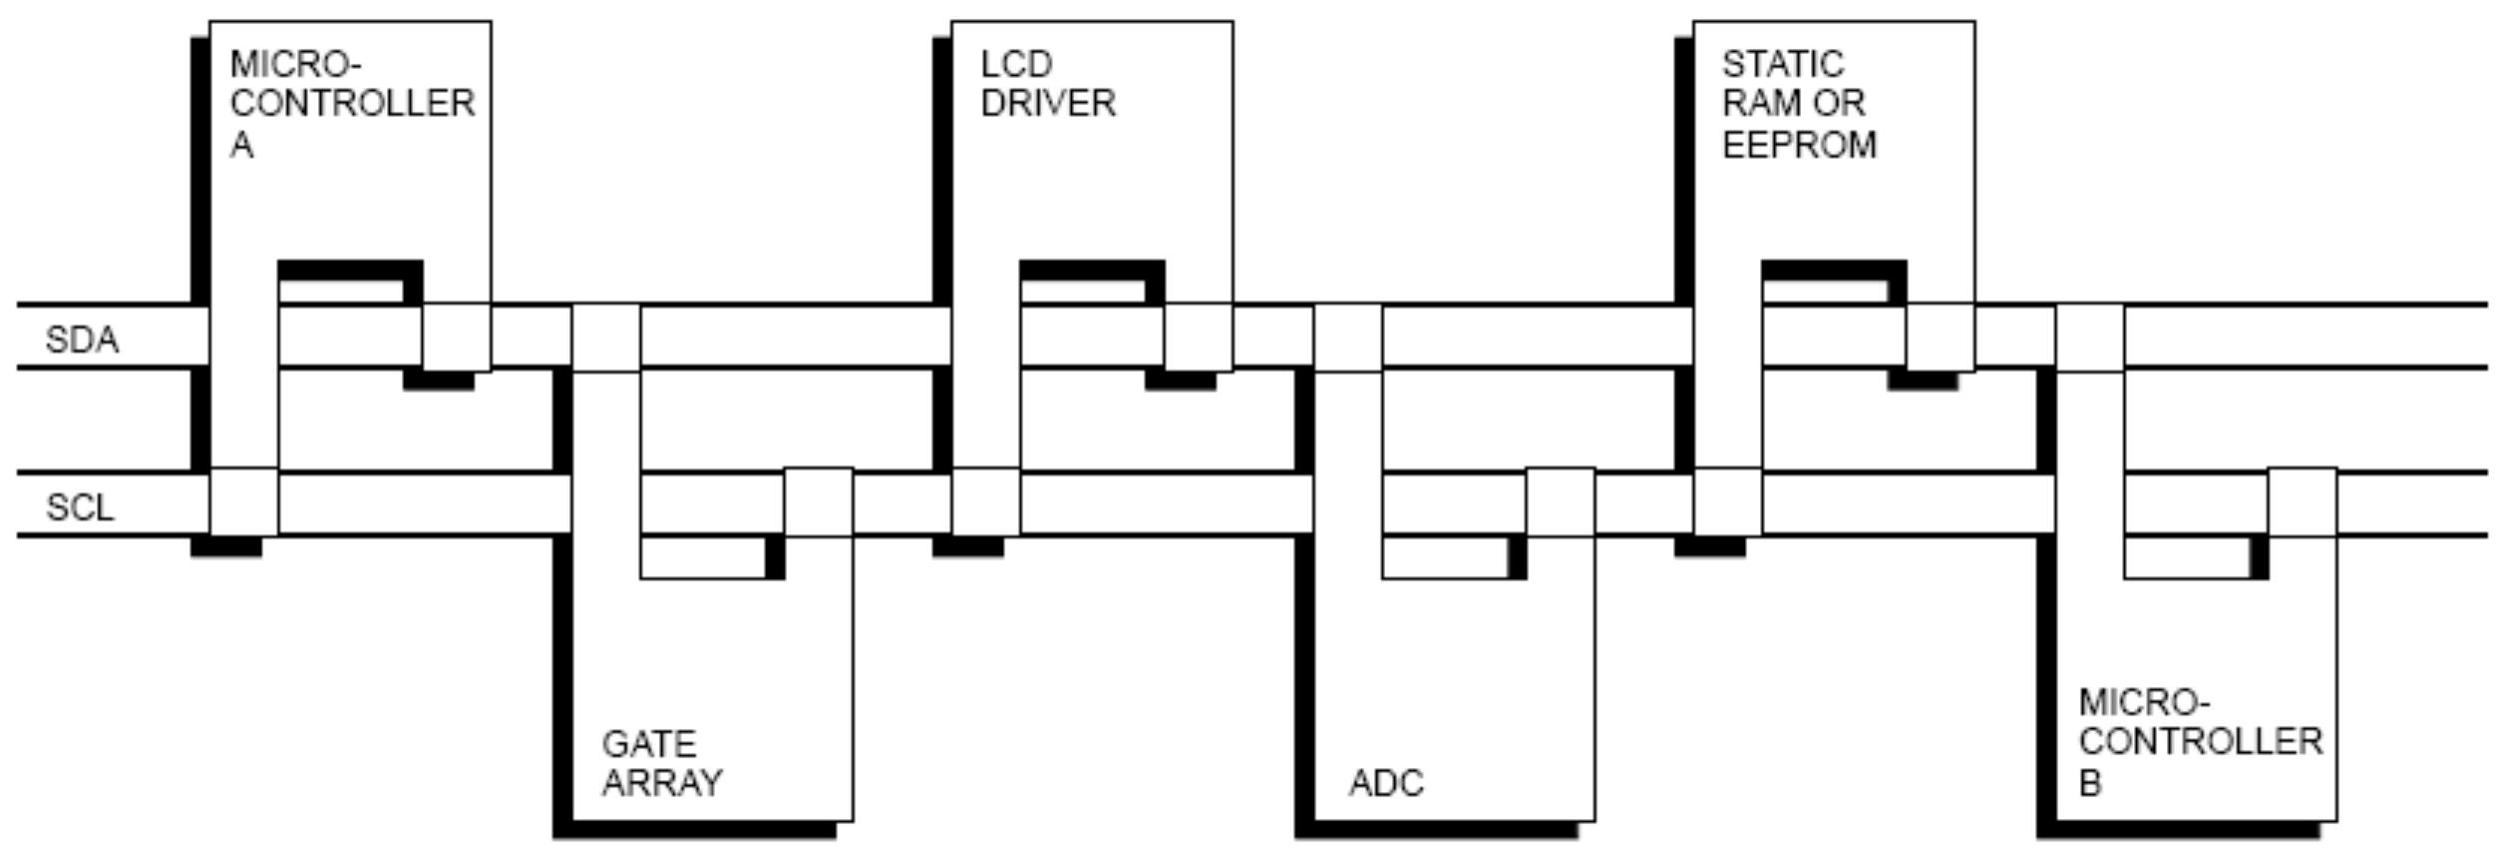
\includegraphics[max width=\textwidth]{2023_01_13_b07e3b4bcffdaab9792bg-246}
\end{center}

Example I2C-connected system with two microcontrollers

(Source: I2C Specification, Philips)

\section{Master-Slave Relationships}
\begin{itemize}
  \item Who is the master?
\end{itemize}

o master-transmitters

o master-receivers

\begin{itemize}
  \item Suppose microcontroller A wants to send information to microcontroller B

  \item A (master) addresses B (slave)

\end{itemize}

o A (master-transmitter), sends data to B (slave-receiver)

o A terminates the transfer.

\begin{itemize}
  \item If microcontroller A wants to receive information from microcontroller B

  \item A (master) addresses microcontroller B (slave)

  \item A (master-receiver) receives data from B (slave-transmitter)

  \item A terminates the transfer

  \item In both cases, the master (microcontroller A) generates the timing and terminates the transfer

\end{itemize}

\section{Exercise: How fast can I2C run?}
\begin{center}
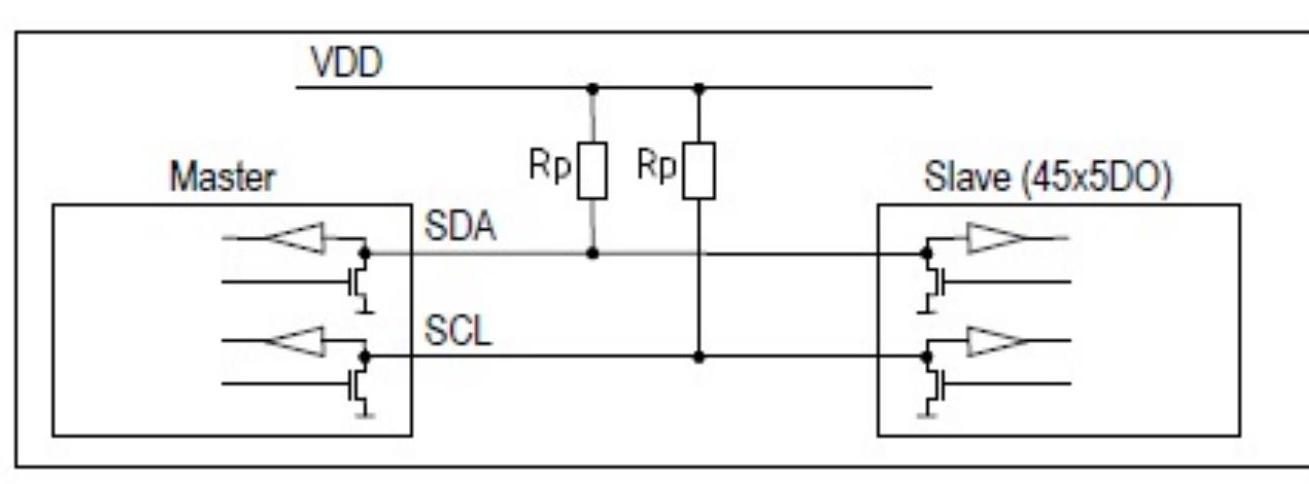
\includegraphics[max width=\textwidth]{2023_01_13_b07e3b4bcffdaab9792bg-248}
\end{center}

Capacitor charging in RC circuit

\begin{center}
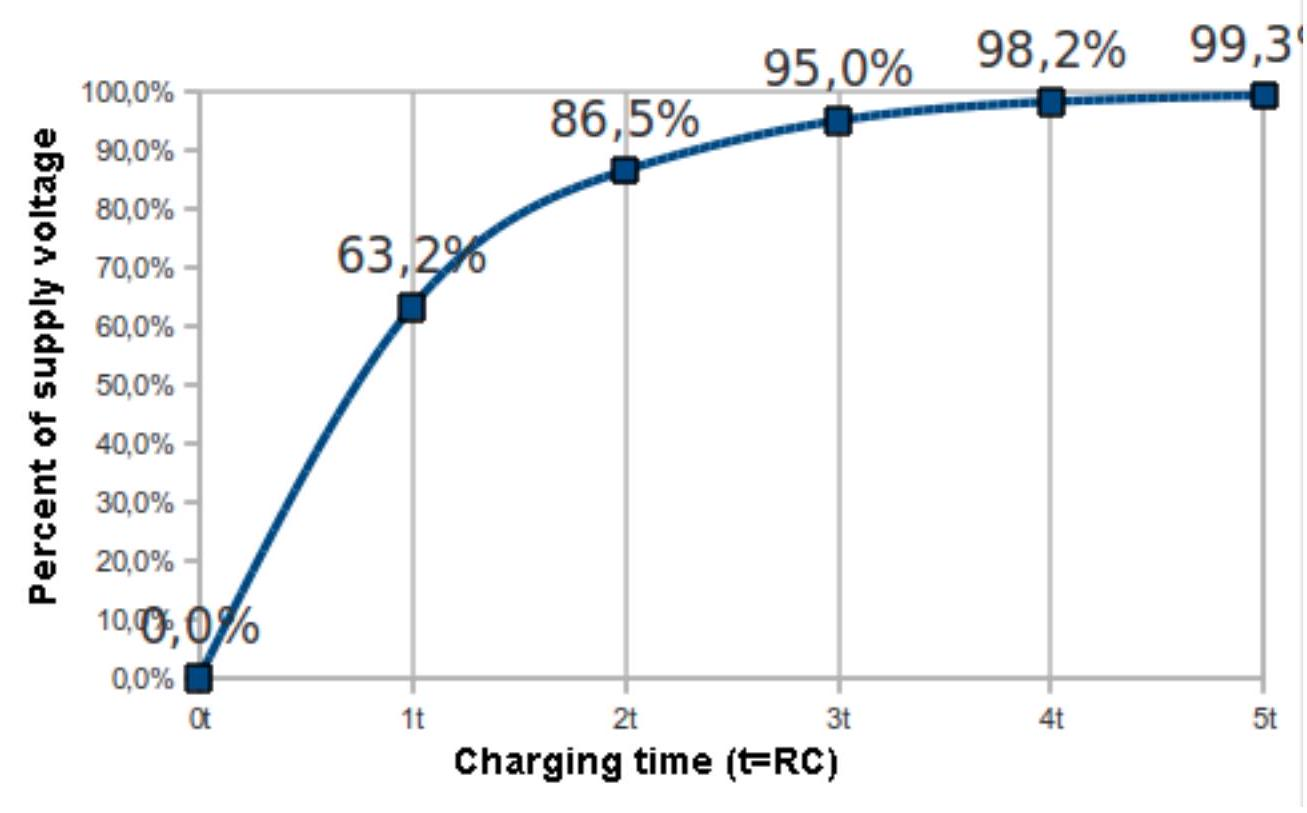
\includegraphics[max width=\textwidth]{2023_01_13_b07e3b4bcffdaab9792bg-248(1)}
\end{center}

\begin{itemize}
  \item How fast can you run it?

  \item Assumptions

  \item 0's are driven

  \item 1's are "pulled up"

  \item Some working figures

  \item $\mathrm{R}_{\mathrm{p}}=10 \mathrm{k} \Omega$

  \item $\mathrm{C}_{\text {cap }}=100 \mathrm{pF}$

  \item $V_{D D}=5 V$
  
  \item $ V_{in_high }=3.5 ~V $
  
  \item Recall for RC circuit
  
\end{itemize}

$-\mathrm{V}_{\text {cap }}(\mathrm{t})=\mathrm{V}_{\mathrm{DD}}\left(1-\mathrm{e}^{-\mathrm{t} / \mathrm{\tau}}\right)$

\begin{itemize}
  \item Where $\tau=R C$
\end{itemize}

\section{Exercise: Bus bit rate vs Useful data rate}
\begin{itemize}
  \item An I2C "transactions" involves the following bits

  \item $\langle\mathrm{S}\rangle\langle\mathrm{A} 6: \mathrm{A} 0\rangle\langle\mathrm{R} / \mathrm{W}\rangle\langle\mathrm{A}\rangle\langle\mathrm{D} 7: \mathrm{D} 0\rangle\langle\mathrm{A}\rangle\langle\mathrm{F}\rangle$

  \item Which of these actually carries useful data?

  \item $\langle\mathrm{S}\rangle\langle\mathrm{A} 6: \mathrm{A} 0\rangle\langle\mathrm{R} / \mathrm{W}\rangle\langle\mathrm{A}\rangle\langle\mathrm{D} 7: \mathrm{D} 0\rangle\langle\mathrm{A}\rangle\langle\mathrm{F}\rangle$

  \item So, if a bus runs at $400 \mathrm{kHz}$

  \item What is the clock period?

  \item What is the data throughput (i.e. data-bits/second)?

  \item What is the bus "efficiency"?

\end{itemize}

\end{document}